\documentclass[letterpaper,11pt]{book}

\usepackage[utf8]{inputenc}
\usepackage[english,russian]{babel}
\usepackage{color}
\usepackage[dvipsnames,svgnames]{xcolor}
\usepackage[a4paper, margin=1in]{geometry}
\usepackage[hang,flushmargin]{footmisc}
\usepackage{dblfnote}
\usepackage{enumitem}
\RequirePackage{cmap}
\usepackage{fontenc}
\usepackage{wrapfig}
\usepackage{longtable}
\usepackage[official]{eurosym}
\usepackage{nicefrac}

\usepackage{lipsum}
\usepackage{tikz}
\usetikzlibrary{backgrounds}
\makeatletter

\tikzset{%
  fancy quotes/.style={
    text width=\fq@width pt,
    align=justify,
    inner sep=1em,
    anchor=north west,
    minimum width=\linewidth,
  },
  fancy quotes width/.initial={.8\linewidth},
  fancy quotes marks/.style={
    scale=5,
    text=white,
    inner sep=1pt,
  },
  fancy quotes opening/.style={
    fancy quotes marks,
  },
  fancy quotes closing/.style={
    fancy quotes marks,
  },
  fancy quotes background/.style={
    show background rectangle,
    inner frame xsep=0pt,
    background rectangle/.style={
      fill=gray!25,
      rounded corners,
    },
  }
}

\newenvironment{fancyquotes}[1][]{%
\noindent
\tikzpicture[fancy quotes background]
\node[fancy quotes opening,anchor=north west] (fq@ul) at (0,0) {``};
\tikz@scan@one@point\pgfutil@firstofone(fq@ul.east)
\pgfmathsetmacro{\fq@width}{\linewidth - 2*\pgf@x}
\node[fancy quotes,#1] (fq@txt) at (fq@ul.north west) \bgroup}
{\egroup;
\node[overlay,fancy quotes closing,anchor=east] at (fq@txt.south east) {''};
\endtikzpicture}

\makeatother

\DFNalwaysdouble % for this example

\usepackage{hyperref}

\hypersetup{
    bookmarks=true, unicode=false,
    pdftoolbar=true, pdfmenubar=true, pdffitwindow=false,
    pdfstartview={FitH}, pdftitle={Russian Vocabulary},
    pdfauthor={P Sopasakis},
    pdfkeywords={}, pdfsubject={Confidential}, 
    pdfnewwindow=true, colorlinks=true, linkcolor=red,
    citecolor=cyan, filecolor=magenta, urlcolor=RoyalBlue
}

\usepackage{parskip}
\setlength{\parindent}{0pt}

\newcommand{\red}[1]{\textcolor{red}{#1}}
\newcommand{\comment}[1]{\textcolor{gray}{\it #1}}
\newcommand{\explain}[2]{\red{#1}\footnote{#1{}:{} #2}}
\newcommand{\explainDetail}[3]{\red{#1}\footnote{#2{}:{} #3}}
\newcommand{\ed}[3]{\red{#1}\footnote{#2{}:{} #3}}


\newenvironment{dialogue}{\list{---}{\it \itemsep=0.05\parskip \topsep=0.75\parskip \parsep=0.75\parskip}}{\endlist}


\title{Сборник текстов\\{\small Газетные и Журнальные Статьи. Тексты об искусстве, истории, музыке, и новостях.}}
\author{Пантелис Сопасакис}

\begin{document}
\maketitle
\tableofcontents


\chapter{Окружающая среда, природа и изменение климата}

\section{Времена года}
\textit{Источник: \url{https://www.memorysecrets.ru/english-texts/vremena-goda-seasons.html}}

Каждое время года имеет свои плюсы и минусы. Давайте детальнее их разберем.

Весна (март, апрель, май) --- самое восхитительное время года. Несмотря на то, что весной \explainDetail{наблюдаются}{(по)наблюдаться}{to be observed} \explainDetail{ливни}{ливень}{shower (rain)}, многие люди \explain{воспринимают}{perceive} весну, как самое лучшее время года. Почему же так \explain{происходит}{happens}? \explain{Дело в том}{the thing is}, весна значит что-то новое для нас. Это шанс начать все заново, изменить жизнь к лучшему. Именно весной рожд\'{а}ется новая жизнь --- \explain{распускаются}{they bloom} почки и начинают цвести цветы.

Лето же (июнь, июль, август) --- это время отдыхать и просто получать удовольствие. Солнце светит с утра до ночи. Взрослые уходят в отпуск, дети --- на каникулы. Большинство людей проводят свои отпуска на море. Там можно не только \explainDetail{загореть}{загорать/загореть}{to tan}, но и встретить много незнакомых людей.

Осень (сентябрь, октябрь, ноябрь) можно разделить на две части --- начало осени и ее конец. В начале осени школьники снова возвращаются к учебе и садятся \explain{за парты}{behind the desks}. Лето постеп\'{е}нно переходит в осень. Но настроение ещё \explain{приподнятое}{elevated}. Вскоре желтые листья начнут осыпаться, и этот величественный пейзаж тоже не \explainDetail{позв\'{о}лит}{позвол\'{я}ть/позв\'{о}лить}{to allow} нам грустить. Втор\'{а}я часть осени не так очаров\'{а}тельна, как первая. Дожди, \explain{сл\'{я}коть}{mud} и грязь --- это то, что люди ненавидят больше всего.

Зима (декабрь, январь, февраль) \explain{на нос\'{у}}{фразеологизм: приближаться, близиться (обычно -- по времени)}, приближаются холода. Мы надеваем перчатки, шапки, шубы и вязаные шарфы. Иногда в эту пору школы закрывают на карантин с целью предотвратить распространение гриппа. Хорошая новость для учеников --- вторые зимние каникулы. Рождество тоже вот-вот наступит. На улице порошит снег, дети лепят снеговиков и играют в снежки. Скоро мы будем наряжать елку, вешать на нее различные шары и гирлянды. Пора встречать Новый год!

\section{Что такое изменение климата?}
\textit{Источник: \url{https://www.un.org/ru/climatechange/what-is-climate-change}}

Под изменением климата понимают \ed{долгосрочные}{долгоср\'{о}чный}{long-term (for a long period)} температурные изменения и изменение погодных \ed{условий}{усл\'{о}вие}{condition}. Хотя эти изменения м\'{о}гут быть естественными, как, например, \ed{циклические}{циклический}{cyclical} \ed{колебания}{колеб\'{а}ние}{fluctuation} солнечной активности, с \ed{1800-х}{1800-х}{тысячи восемьсотых} годов антропогенная деятельность является основным \explain{движущим фактором}{driving factor} изменения климата, \explain{главным образом}{mainly} за счёт \ed{сжигания}{сжигание}{burning; combustion} ископаемых видов топлива, таких как уголь, нефть и газ.

В результате сжигания ископаемых видов топлива образуются \explain{выбросы}{emissions} \ed{парниковых газов}{парник\'{о}вые г\'{а}зы}{greenhouse gases}, которые подобно одеялу \explain{окутывают}{they envelop} Землю, удерживая солнечное тело и \explain{повышая}{raising} температуру.

Примерами парниковых газов, выбросы которых вызывают изменение климата, являются \explain{дву\'{о}кись углер\'{о}да}{углекислый газ} и мет\'{а}н. Они образуются, например, при использовании бензина для езды на автомобилях или угля для отопления зданий. \explain{Расчистка земель и лесов}{the ``clearing'' of lang and forest} также может привести к \ed{высвобождению}{высвобожд\'{е}ние}{release} углекислого газа.
Главным источником выбросов метана являются \explain{м\'{у}сорные св\'{а}лки}{garbage dumps}.
К числу основных производителей выбросов относятся энергетика, промышленность, транспорт, здания, сельское хозяйство и землеп\'{о}льзование.

\begin{fancyquotes}
    Концентрация парниковых газов находится на самом высоком уровне за последние 2 миллиона лет
\end{fancyquotes}

И выбросы продолжают расти! В результате этого сейчас Земля на \explain{1,1°C}{одна целая, одна десятая градуса Цельсии} теплее, чем в конце 1800-х годов. Прошедшее десятилетие (2011–2020 г\'{о}ды) было самым тёплым в истории.

Хотя многие думают, что изменение климата означает в основном более высокие температуры, рост температуры -- это только начало истории. Поскольку Земля -- это система, где всё \explain{взаимосв\'{я}зано}{interconnected}, изменения в одной \explain{сфере}{here: area} могут повлиять на изменения во всех остальных.

В настоящее время к последствиям изменения климата относят, \explain{среди прочего}{among other things}, сильные \ed{з\'{а}сухи}{з\'{а}суха}{drought}, \explain{нехватку воды}{water shortage}, сильные пожары, повышение уровня моря, наводнения, \explain{т\'{а}яние}{melting (n.)} полярных льдов, катастрофические штормы и сокращение \ed{биоразнообр\'{а}зия}{биоразнообр\'{а}зие}{biodiversity}.

\begin{fancyquotes}
    Люди ст\'{а}лкиваются с различными последствиями изменения климата
\end{fancyquotes}

Изменение климата может \ed{сказ\'{а}ться}{ск\'{а}зываться/сказ\'{а}ться + на что}{affect} на нашем здоровье, способности \explain{выращивать}{to grow} \explain{продовольственные культуры}{food crops}, жильё, безопасности и работе.
Некоторые из нас уже сейчас более \ed{уязв\'{и}мы}{уязв\'{и}мый}{vulnerable} к \ed{воздействию}{возд\'{е}йствие}{impact (n)} изменения климата, например, люди, живущие в малых \ed{островн\'{ы}х}{островн\'{о}й}{insular} государствах и других развивающихся странах. Такие последствия, как повышение уровня моря и интрузия соленых вод, дост\'{и}гли такого уровня, что целые общ\'{и}ны были в\'{ы}нуждены \explain{пересел\'{и}ться}{to resettle}, а затяжные засухи \explain{подвергают}{subject; expose} людей риску г\'{о}лода. В будущем ожидается рост числа «климатических беженцев».

\begin{fancyquotes}
    Каждый дополнительный градус \ed{глобального потепления}{глобальное потепление}{global warming} \explain{имеет значение}{matters}
\end{fancyquotes}

В докладе Организации Объединённых Наций за 2018 год тысячи учёных и \ed{правительственных экспертов}{прав\'{и}тельственный эксп\'{е}рт}{gov't expert} согласились с тем, что \explain{ограничение}{limitation} роста глобальной температуры на уровне не более 1,5°C поможет нам избежать самых худших климатических последствий и \explain{сохранить}{save} кл\'{и}мат, \explain{приг\'{о}дный для жизни}{habitable}. Однако, согласно текущим национальным климатическим планам, ожидается, что глобальное потепление дост\'{и}гнет 2,7°C к концу столетия.

Хотя выбросы, вызывающие изменение климата, образуются во всех регионах мира и сказываются на всех, некоторые страны производят их в гораздо больших объёмах, чем другие. В то время как на 100 стран, которые производят меньше всего выбросов, приходится 3 процента от общего объема выбросов, \explain{доля}{share (n)} десяти стран, являющихся самыми крупными производителями выбросов, составляет 68 процентов. Хотя принятие мер по борьбе с изменением климата -- это дело всех и каждого, народы и страны, которые создают больше проблем, должны взять на себя большую ответственность и начать действовать первыми.

\begin{fancyquotes}
    Мы сталкиваемся с огромным \ed{вызовом}{вызов}{challenge}, но нам уже известны многие решения
\end{fancyquotes}

Многие решения в области изменения климата могут быть не только экономически выгодными, но и также улучшить нашу жизнь и защитить окружающую среду. У нас также есть глобальные структуры и соглашения, на основе которых осуществляются \ed{усилия}{усилие}{effort}, направленные на достижение прогресса, такие как цели в области \ed{устойчивого развития}{устойчивый развитие}{sustainable development}, Рамочная конвенция Организации Объединённых Наций об изменении климата и Парижское соглашение. Имеются три широкие категории действий: сокращение выбросов, адаптация к последствиям изменения климата и финансирование необходимых мер по адаптации.

\explain{Перевод}{Translation (meaning transition)} энергетических систем с ископаемого топлива на использование \ed{возобновляемых источников энергии}{возобновляемые источники энергии}{renewable energy sources}, таких как солнце или ветер, позв\'{о}лит сократить выбросы, вызывающие изменение климата. Но начинать нужно прямо сейчас. Несмотря на расширение коалиции стран, \explain{обязавшихся}{who pledged} достичь чистого нулевого уровня выбросов к 2050 году, около половины мер по сокращению выбросов должны быть осуществлен\'{ы} к 2030 году, с тем чтобы удержать потепление на уровне ниже 1,5°C. В период с 2020 по 2030 год производство ископаемого топлива должно сокращаться прим\'{е}рно на 6 процентов в год.

Цель адаптации к последствиям изменения климата состоит в том, чтобы защитить людей, их жилища, предприятия, источники средств к существованию, инфраструктуру и природные экосистемы. Эта деятельность касается не только нынешних последствий, но и тех, с которыми, вероятно, придётся столкнуться в будущем. Хотя меры по адаптации придётся принимать \explain{повсеместно}{everywhere}, в настоящее время приоритетное внимание необходимо уделять наиболее уязв\'{и}мым сло\'{я}м населения, у которых меньше всего ресурсов для того, чтобы \explain{противостоять}{resist} климатическим угр\'{о}зам. Это может \explain{окупиться}{pay off} \explain{сполна}{completely}. Например, системы раннего предупреждения \ed{стихийных бедствий}{стихийное бедствие}{natural disaster} спасают жизни и имущество и могут принести выгоды, в десятки раз превышающие первоначальные \explain{затраты}{costs}.

\begin{fancyquotes}
    Мы можем оплатить счет сейчас или дорого заплатить в будущем
\end{fancyquotes}

Меры по борьбе с изменением климата требуют значительных финансовых \ed{вложений}{вложение}{investment} со стороны правительств и делов\'{ы}х кругов. Однако \explain{бездействие}{inaction} в отношении климата обходится гораздо дороже. Одним из важнейших шагов является выполнение \ed{промышленно развитыми странами}{промышленно развитая стран\'{а}}{industrialised countries} своих обязательств по предоставлению 100 миллиардов долларов в год \ed{развивающимся странам}{развив\'{а}ющаяся стран\'{а}}{developing country}, с тем чтобы они могли адаптироваться и перейти к более «зеленой» экономике.



\section{Причины изменения климата}
\textit{Источник: \url{https://www.un.org/ru/science/causes-effects-climate-change}}



\textbf{Производство электроэнергии}

Значительная доля глобальных выбросов связана с производством электроэнергии и тепла путем сжигания ископаемых видов топлива. Бóльшая часть электроэнергии по-прежнему производится посредством сжигания угля, нефти или газа, в результате чего образуются углекислый газ и закись азота – мощные парниковые газы, которые покрывают Землю и \explain{задерживают}{trap; hold} солнечное тепло. Во всем мире чуть более четверти электроэнергии вырабатывается \explain{за счёт}{here it means ``by means of,'' but it can also mean ``at the expense of.''} ветра и солнца и поступает из других возобновляемых источников, которые, в отличие от ископаемых видов топлива, практически не \explain{выделяют}{emit} в атмосферу парниковых газов или \ed{загрязняющих веществ}{загрязняющее вещество}{pollutant}.

\textbf{Изготовление\footnote{изготовление: manufacturing} товаров}

Предприятия обрабатывающей и других отраслей промышленности производят выбросы, в большинстве случаев являющиеся результатом сжигания ископаемых видов топлива в целях выработки энергии, необходимой для получения цемента, железа, стали, электронных устройств, \ed{пластмасс}{пластм\'{а}сса}{plastic}, одежды и других товаров.
При добыче полезных ископаемых и других промышленных процессах, \explain{равно как}{as well as} и при строительстве, также выделяются газы. Машины, используемые в производственном процессе, \explain{зачаст\'{у}ю}{often} работают на угл\'{е}, нефти или газе, а некоторые материалы, такие как пластмассы, производятся из химических веществ, получаемых из ископаемых видов топлива. Обрабатывающая промышленность является одним из крупнейших источников выбросов парниковых газов в мире.

\textbf{Вырубка лесов\footnote{в\'{ы}рубка лес\'{о}в: deforestation}}

В результате вырубки лесов для создания ферм или пастбищ либо по иным причинам образуются выбросы, поскольку вырубаемые деревья высвобождают накопленный углерод. Ежегодно уничтожается около 12 млн гектаров леса. Поскольку леса \explain{поглощают}{absorb} углекислый газ, их уничтожение также ограничивает способность природы удерживать выбросы в атмосферу. \ed{Обезл\'{е}сение}{обезл\'{е}сение}{deforestation} \explain{наряду с}{along with; alongside} сельским хозяйством и другими изменениями в землепользовании является причиной примерно четверти глобальных выбросов парниковых газов.

\textbf{Использование транспорта}

Большинство автомобилей, грузовиков, кораблей и самолётов работают на ископаемых видах топлива. Это делает транспорт одним из главных источников выбросов парниковых газов, особенно выбросов углекислого газа. Наибольшая их часть приходится на дорожные транспортные средства в связи со сжиганием продуктов нефтепереработки, таких как бензин, в двигателях внутреннего сгорания. При этом выбросы морск\'{и}х и воздушных суд\'{о}в продолжают расти. На транспорт приходится почти четверть глобальных выбросов углекислого газа, связанных с энергоснабжением. \explain{Существующие тенденции}{Existing trends} \explain{указывают на}{indicate} вероятность значительного увеличения энергопотребления в транспортном секторе в ближайшие годы.

\textbf{Производство продуктов питания}

Производство продуктов питания прив\'{о}дит к выбросам углекислого газа, метана и других парниковых газов разными путями, включая вырубку лесов и расчистку земель для ведения сельского хозяйства и выпаса скота, работу пищеварительных систем коров и овец, производство и применение удобрений и навоза для выращивания сельскохозяйственных культур и использование энергии для эксплуатации сельскохозяйственного оборудования или рыболовецких судов, обычно работающих на ископаемых видах топлива. Все это делает производство продуктов питания одним из основных факторов, способствующих изменению климата. Выбросы парниковых газов также связаны с \ed{упаковкой}{упаковка}{packaging} и \ed{распростран\'{е}нием}{распростран\'{е}ние}{here: distribution} продуктов питания.

\textbf{Энергоснабжение зданий\footnote{энергоснабжение зданий: energy supply of buildings}}

В мировом масштабе жил\'{ы}е и коммерческие здания потребляют более половины всей электроэнергии. В связи с продолжающимся использованием угля, нефти и природного газа для целей отопления и \ed{охлаждения}{охлаждение}{cooling} они выбрасывают значительные количества парниковых газов. В последние годы повышение \ed{спроса}{спрос}{demand} на энергию для \ed{отопления и охлаждения}{отопление и охлаждение}{heating and cooling} с р\'{о}стом ч\'{и}сленности влад\'{е}льцев \ed{кондиционеров}{кондицион\'{е}р}{air conditioner} и увеличение потребления электричества для \ed{освещения}{освещение}{lighting} и обеспечения работы бытовой техники и подключенных устройств способствовали увеличению выбросов углекислого газа, производимых зданиями и связанных с энергоснабжением.

\textbf{Слишком интенсивное потребление}

Ваш дом и использование электроэнергии, то, как вы передвигаетесь, то, что вы едите, и количество того, что вы выбрасываете, влияют на выбросы парниковых газов. Это же можно сказать о потреблении таких товаров, как одежда, электронные устройства и пластмассы. Значительная часть глобальных выбросов парниковых газов связана с частными домохозяйствами. Наш образ жизни оказывает глубокое воздействие на нашу планету. Самые \explain{состоятельные}{состоятельный}{wealthy; well-off} л\'{и}ца несут наибольшую ответственность\footnote{Recall: нести ответственность: to have responsibility}: на 1 процент самых богатых жителей планеты в совокупности приходится больше выбросов парниковых газов, чем на 50 процентов беднейшего населения.

На основе различных источников ООН


\section{Последствия изменения климата}
\textit{Источник: \url{https://www.un.org/ru/science/causes-effects-climate-change}}


\textbf{Повышение температур}

С увеличением концентрации парниковых газов растёт и глобальная температура земной поверхности. Последнее десятилетие --- 2011–2020 годы --- стало самым тёплым за всю историю наблюдений. С 1980-х годов каждое десятилетие было теплее предыдущего. Почти во всех районах суши наблюдается увеличение количества жарких дней и периодов аномальной жары. Повышение температуры увеличивает количество заболеваний, связанных с жарой, и затрудняет работу на открытом воздухе. Природные пожары легче возникают и быстрее распространяются в более жарких условиях. Температура в Арктике повышалась по крайней мере вдвое быстрее, чем в среднем по миру.

\textbf{Усиление штормов}

Многие регионы \ed{столкн\'{у}лись}{ст\'{а}лкиваться/столкн\'{у}ться + с}{were faced with} с увеличением интенсивности и частоты \ed{разрушительных}{разрушительный}{destructive} штормов. При повышении температуры \explain{испаряется}{evaporates} больше \ed{влаги}{влага}{humidity}, что усиливает ливневые дожди и наводнения, вызывая более опасные штормы. На частоту и масштабы тропических штормов также влияет потепление океана. Циклоны, ураганы и тайфуны формируются в тёплых водах у поверхности океана. Такие ураганы нередко разрушают дом\'{а} и \explain{населенные пункты}{populated areas; settlements}, становясь причиной гибели людей и огромных экономических потерь.

\textbf{Усиление з\'{а}сухи}

Изменение климата меняет степень доступности воды, делая её более дефицитным ресурсом в растущем числе регионов. Глобальное потепление усугубляет нехватку воды в регионах, и без того испытывающих её дефицит, и увеличивает риск сельскохозяйственных засух, влияющих на урожай, и экологических засух, повышающих уязвимость экосистем. Засухи также могут вызывать разрушительные \explain{песчаные}{sandy} и пыльные бури, способные перемещать миллиарды тонн песка через континенты. Пустыни расширяются, сокращая площадь земель для выращивания продовольственных культур. Сегодня многие люди постоянно сталкиваются с угр\'{о}зой нехватки воды.

\textbf{Потепление и повышение уровня океана}

Океан \explain{поглощает}{absorbs} бóлчьшую часть тепла, образующегося в процессе глобального потепления. За последние двадцать лет скорость, с которой океан \explain{нагревается}{heats up}, сильно возросла на всех его глубинах. По мере потепления океана его объём увеличивается, поскольку при нагревании вода расширяется. Таяние ледовых щитов также приводит к повышению уровня моря, \explain{угрожая}{threatening} прибрежным и островным сообществам. Кроме того, океан поглощает из атмосферы углекислый газ. При этом увеличение количества углекислого газа повышает кислотность океана, что ставит под угрозу морскую флору и ф\'{а}уну и коралловые рифы.

\textbf{Исчезновение видов}

Изменение климата создает риски для выживания видов на суше и в океане. Эти риски возрастают по мере повышения температуры. Мир, положение в котором усугубляется изменением климата, теряет виды в тысячу раз быстрее, чем когда-либо в письменной истории человечества. Миллион видов находится под угрозой исчезновения в течение следующих нескольких десятилетий. В число многочисленных угроз, связанных с изменением климата, входят лесные пожары, экстремальные погодные условия и инвазивные вредители и заболевания. Некоторые виды смогут сменить место обитания и выжить, а другие нет.

\textbf{Нехватка продуктов питания}

В группу причин глобального роста распространенности голода и неполноценного питания входят климатические изменения и увеличение количества экстремальных погодных явлений. Рыбные ресурсы, сельскохозяйственные культуры и домашний скот могут быть уничтожены или стать менее продуктивными. В связи с закислением океана морские ресурсы, обеспечивающие питание для миллиардов людей, находятся под угрозой. Изменения снежного и ледяного покрова во многих арктических регионах нарушили систему снабжения продовольствием, обеспечиваемым за счет пастбищного животноводства, охоты и рыболовства. Тепловой стресс может уменьшать количество воды и пастбищ, что приводит к снижению урожайности сельскохозяйственных культур и негативным образом сказывается на поголовье скота.

\textbf{Увеличение рисков для здоровья}

Изменение климата – это самая большая угроза для здоровья людей. Его последствия уже наносят вред здоровью в связи с загрязнением воздуха, распространением заболеваний, возникновением экстремальных погодных явлений, вынужденным перемещением, оказанием давления на психику и обострением проблем голода и неполноценного питания в местах, где люди не могут выращивать продовольственные культуры или обеспечить наличие достаточного количества пищевых продуктов. Экологические факторы ежегодно уносят жизни около 13 млн человек. Изменение погодных условий приводит к распространению заболеваний, а экстремальные погодные явления увеличивают смертность и затрудняют работу систем здравоохранения.

\textbf{Нищета и вынужденное перемещение}

Изменение климата усиливает факторы, ввергающие людей в нищету и не позволяющие им исправить ситуацию, в которой они оказались. Наводнения могут смести городские трущобы, разрушив дома и уничтожив источники средств к существованию. Жара может затруднить работу на открытом воздухе. Нехватка воды может повлиять на урожай. В последние десять лет (2010–2019 годы) связанные с погодой явления приводили к вынужденному перемещению в среднем около 23,1 млн человек в год, повышая риск оказаться в нищете для еще большего числа людей. Большинство беженцев прибывают из самых уязвимых стран, наименее готовых адаптироваться к последствиям изменения климата.

\textit{На основе различных источников ООН}


\section{Человечество ждёт серия масштабных природных катастроф}

\textit{В чем причина стихийных бедствий ближайшего будущего?}

\textit{Источник: \url{https://lenta.ru/articles/2022/10/17/trilliondollarbaby/}}

В скором будущем человечество ожидает уникальное для этого столетия явление. Так называемая Ла-Нинья — феномен, с которым связано широкомасштабное охлаждение вод Тихого океана, — грозит оказаться тройной. Последствия Ла-Ниньи, чье название с испанского можно перевести как «девочка», могут стать катастрофическими. Если прогноз сбудется, хаос природных катаклизмов на планете только усилится. В таком сценарии глобальный ущерб от стихийных бедствий достигнет триллиона долларов. Роковая «малышка» — в материале «Ленты.ру».

\textbf{Горячо-холодно.} Нынешняя затяжная Ла-Нинья началась в сентябре 2020 года. Явление уже успело усугубить засуху и наводнения в различных частях мира, а теперь же Всемирная метеорологическая организация (ВМО) предупредила, что явление затянется надолго. С вероятностью в 70 процентов оно сохранится до ноября, с вероятностью в 55 процентов — до февраля следующего года.

Ситуация, как подчеркнул генеральный секретарь ВМО Петтери Таалас, складывается исключительная. В нынешнем столетии природный феномен может охватить сразу три зимы в Северном полушарии и три лета в Южном. Если прогноз ВМО окажется верным, то тройная Ла-Нинья станет третьей по счету за всю историю наблюдений — с 1950 года подобное случалось лишь дважды.

Ла-Нинья (исп. La Niña — малышка, девочка) — это снижение температуры поверхностных вод в центральной и восточной частях Тихого океана. На этом фоне усиливаются стабильные восточные ветра, которые гонят теплую воду от берегов Перу и Чили в сторону Индонезии и Австралии. В результате средние температуры воздуха во всем мире понижаются.

Явление с противоположным эффектом, когда температура воды и воздуха у побережья Южной Америки растет, называют Эль-Ниньо (исп. El Niño — малыш, мальчик), а его чередование с Ла-Ниньей — Южной осцилляцией. Феномен описал британский ученый Гилберт Уокер в 1923 году, однако впервые на него обратили внимание перуанские рыбаки в 1600 годах — Ла-Нинья для них не имела критического значения, но потепление воды при Эль-Ниньо плохо сказывалось на уловах.

На климат нашей планеты Ла-Нинья оказывает охлаждающий эффект, который достигает своего максимума на второй год после ее пика. Характерными проявлениями феномена метеорологи называют прохладную и влажную зиму на севере Европы и в Великобритании, дождливое лето в Индонезии и Австралии, сильные муссоны (ветры, дующие с суши на океан) в Юго-Восточной Азии, холода в Южной части Африки. В этот период зима на Дальнем Востоке в России, в Японии, Корее, Канаде, на севере США обычно бывает более снежной и ветреной. В Техасе, Флориде и других южных штатах Америки, наоборот, случаются сильные засухи.

При этом связанное с деятельностью человека изменение климата, как отмечают ученые, усиливает воздействие Южной осцилляции на окружающую среду. ВМО выяснила, что за последние 50 лет число стихийных бедствий пятикратно увеличилось.

\begin{fancyquotes}
    Это означает более длительные и интенсивные волны тепла, более длительные засухи, более масштабные лесные пожары и более разрушительные наводнения. Усиленный изменением климата эффект от Ла-Ниньи носит глобальный характер

    \begin{flushright}
        Билл Пацертамериканский \\
        океанограф и климатолог
    \end{flushright}
\end{fancyquotes}

По словам ученой из Национального управления океанических и атмосферных исследований при министерстве торговли США Антониетты Капотонди, сила воздействия Южной осцилляции на климат непредсказуема — не наблюдалось двух абсолютно одинаковых по эффекту Эль-Ниньо и Ла-Ниньи. «Мы видели, насколько разнообразными могут быть последствия Южной осцилляции. Эта вариативность усложняет прогнозы по влиянию изменения климата на будущие Эль-Ниньо и Ла-Нинья», — пояснила исследовательница.

Ученые предполагают, что явления Эль-Ниньо и Ла-Нинья в перспективе будут случаться чаще. На фоне активного загрязнения планеты выбросами парниковых газов к концу XXI века они будут возникать не один раз в 20 лет, а раз в десятилетие. При этом осадки сместятся на восток вдоль экваториальной части Тихого океана во время Эль-Ниньо и на запад во время последствий Ла-Ниньи.

При увеличении периодичности и амплитуды Южной осцилляции экстремальные погодные явления будут более выраженными. Некоторые эффекты воздействия глобального потепления на протекание Эль-Ниньо и Ла-Ниньи уже стали очевидными — к примеру, тихоокеанские штормы заметно участились и усилились. В 2020 году зафиксировали рекордные 30 таких ураганов, в 2021-м — 21, а в 2022 — 14.

\textbf{Всем досталось.} Связанные с Ла-Ниньей экстремальные погодные условия затронули многие регионы планеты. Так, засуха накрыла западные части США и Канады, практически опустошив находящиеся на этих территориях водоемы. В результате возник дефицит пресной воды — ее не хватает ни для поливов сельскохозяйственных земель, ни для производства энергии на гидроэлектростанциях. В частности, в Техасе засуха привела к огромным потерям урожая хлопка — цены на него достигли десятилетнего максимума в начале 2022 года. По словам главного исполнительного директора компании Plains Cotton Growers Inc Коди Бессета, долговременная жара вкупе с практическим отсутствием осадков рискуют сделать 2022 год самым сложным для производства сельскохозяйственных культур. Эксперт прогнозирует, что производители недосчитаются более половины привычного объема урожая.

Продолжительная сухая погода также нанесла ущерб урожаю кофе, сахара и апельсинов в Бразилии, которая считается крупнейшим в мире экспортером этих трех культур. Помимо этого, экстремальные погодные условия нарушили работу предприятий по добыче железной руды в стране — в том числе второго по величине в мире производителя Vale SA.

В Аргентине засуха сказалась на посевах сои и кукурузы, которые играют ключевую роль в торговом балансе страны, переживающей острый экономический кризис. Многолетняя нехватка осадков также высушила ключевой водный путь — реку Парану. Поэтому фермеры и продавцы сельхозтоваров столкнулись с дополнительными расходами на логистику — им приходится платить внушительные суммы за отправку товаров через альтернативные порты.

На Австралию, наоборот, обрушились проливные дожди. Ливнями затопило большую часть штатов Новый Уэльс, Квинсленд и Виктория. Наводнения привели к гибели более 20 человек и разрушили более 15 тысяч домов. Страховые выплаты при этом превысили три миллиарда долларов.

Сильные дожди негативно сказались на качестве урожая уже выросших зерновых культур, а также задержали время посева ячменя и пшеницы. Кроме того, от разлива водоемов под угрозой выхода из строя оказались металлургические шахты в Новом Южном Уэльсе и Квинсленде — они являются крупнейшими в мире экспортерами сырья для производства стали. Другим катастрофическим последствием стала гибель животных. Так, связанные с Ла-Ниньей теплые течения в сторону востока погубили пингвинов, которых массово выбросило на пляжи Новой Зеландии.

Пакистан вызванные Ла-Ниньей обильные ливни поставили под угрозу дефолта. Страна подверглась беспрецедентным наводнениям, в результате которых были разрушены десятки миллионов домов, погибло почти 1500 человек. Кроме того, чрезмерные осадки повредили более 70 процентов посевов риса в провинции Синд. Нанесенный стихийными бедствиями ущерб аналитики оценивают в 30 миллиардов долларов. Южноазиатская страна и так страдает от сокращения валютных резервов и самой высокой инфляции за последние десятилетия, а природные факторы лишь усугубят тяжелое экономическое положение.

По данным Международной федерации обществ Красного Креста и Красного Полумесяца, разрушительные наводнения случились также в Бангладеш и Индии — от них пострадали более 7,2 миллиона человек и оказались поврежденными более 300 тысяч домов.

\textbf{Час расплаты.} Эксперты убеждены, что связанные с Ла-Ниньей погодные циклы усугубляют уже существующие глобальные проблемы. «Когда добавляются экстремальные погодные условия, это просто создает сценарий для более высоких цен на энергию, более высоких цен на продукты питания и большей инфляции. Это негативно для мировой экономики», — пояснил президент и основатель Pento Portfolio Strategies Майкл Пенто.

Ущерб от вызванных Ла-Ниньей засух, штормов и наводнений аналитики оценивают в десятки миллиардов долларов. Однако в этот раз природные катаклизмы случались так часто в разных уголках планеты, что реальную сумму потерь сложно вычислить. Получить представление о размере ущерба можно на основании данных страховых компаний. Как сообщают в аналитической и консалтинговой фирме Aon, в 2020 году стихийные бедствия обошлись миру в 268 миллиардов долларов, а в 2021-м — в дополнительные 329 миллиардов долларов.

\begin{center}
    {\Huge
        1 триллион долларов
    }

    {\Large
        составит глобальный ущерб от последствий Ла-Ниньи
    }
\end{center}

Если будущий масштаб стихийных бедствий окажется соизмеримым с прошлыми годами, то к концу 2023-го сумма ущерба от Ла-Ниньи может достичь или даже превысить один триллион долларов. При этом речь идет не только о повреждении имущества и потерях урожая. От погодных условий зависят цены на разные товары по всему миру — от чашки кофе до угля, который используют для производства стали. Помимо войн, Ла-Нинья — единственное событие, оказывающее влияние на глобальные рынки и почти все отрасли экономики, считают эксперты.

\textbf{Выход есть?} Сократить риск негативных для планеты последствий явления можно за счет снижения антропогенного воздействия на климат — сокращения уровня эмиссии парниковых газов. Для этого, прежде всего, необходимо отказаться от использования ископаемого топлива — угля, нефти, природного газа и прочих горючих минералов — в пользу возобновляемых источников энергии, таких как солнечный свет, ветер и вода.

На протяжении нескольких десятилетий лидирующие позиции по энергопереходу занимает Евросоюз (ЕС) — в странах блока заметная доля в энергобалансе приходится на зеленые источники. Власти ЕС также поставили амбициозные цели по спасению планеты. Согласно опубликованной в 2021 году стратегии по борьбе с изменением климата, к 2030 году выбросы парниковых газов на территории Европы должны сократиться на 55 процентов относительно уровня 1990 года, а к 2050-му — быть полностью компенсированы.

Однако специальная военная операция России, начатая в феврале на Украине, вынудила ЕС поступиться важной целью. Блок стран резко сократил импорт дешевого российского газа (с 40 процентов в 2021 году до 7 процентов от общего объема) и столкнулся с энергетическим кризисом, так как существующих солнечных, ветряных и гидроэлектростанций недостаточно для обеспечения бесперебойной подачи тепла и света. Чтобы компенсировать нехватку, Европе пришлось вернуться к использованию сильно вредящих планете угля и мазута.

Все это делает недостижимыми цели Парижского соглашения по климату, которое подразумевает сдерживание роста среднемировых температур на отметке 1,5 градуса Цельсия относительно доиндустриального уровня. По прогнозам ученых, даже без учета наихудших сценариев средняя температура на планете повысится от 2,1 до 3,9 градуса Цельсия к 2100 году.

Межправительственная группа экспертов по изменению климата ООН уже предрекла человечеству неминуемую глобальную катастрофу. По прогнозам ученых, повышение температуры на планете в ближайшие десятилетия достигнет критических значений для сельского хозяйства и здравоохранения, а эффект глобального потепления ощутят на себе все страны мира.

Поскольку рост среднемировых температур продолжается, а глобальные выбросы СО2 не сокращаются, вероятно, Эль-Ниньо и Ла-Нинья станут лишь усиливаться, а вместе с ними увеличится и число катастрофических явлений. Среди угроз — более интенсивные дожди, наводнения, сильнейшая засуха во многих регионах, лесные пожары, опасность для прибрежных территорий из-за подъема уровня Мирового океана, усиление таяния вечной мерзлоты. Все это способно привести к затяжным экономическим кризисам, массовым проблемам со здоровьем и гибели людей и животных.

\section{Городск\'{а}я жизнь}
Вы никогда не думали о последствиях жизни в городе? Казалось бы, \explain{на первый взгляд}{at first sight}, что жизнь в больших экономических и культурных центрах имеет только преимущества, но дальнейшее рассмотр\'{е}ние показывает, что она имеет и \explain{недостатки}{недостаток: disadvantage}.

С \explain{положительной}{полож\'{и}тельный/-ая: positive} стороны, легче найти работу в городе, потому что там обычно много ресторанов, кафе, гостиниц, школ, библиотек, музеев и т.д. Кроме того, жители города имеют прекрасную возможность посетить множество культурных и развлекательных учреждений, таких как музеи, галереи, ночные клубы, дискотеки и многое другое.

С другой стороны, жителям города \explain{приходится}{приходиться/прийтись: have to} жить в загрязненной атмосфере из-за интенсивного автомобильного движения и \explain{промышленных}{industrial} \explain{предприятий}{предпри\'{я}тие: enterprise}. Это может \explain{вызвать}{to cause} \explain{заболевания}{disease} лёгких и проблемы с сердцем. Кроме того, городской образ жизни довольно \explain{напряженный}{intense}, \explain{поскольку}{since/because} приходится много работать, много ездить на автомобиле и, в результате, стоять в пробках...

В заключение, городская жизнь имеет некоторые преимущества. Тем не менее, она также \explain{может нанести ощутимый вред}{can cause significant damage}, так что местные власти должны сделать несколько важных решений, например, они должны \explain{запретить}{[запрещать] to ban} промышленные предприятия в городах и вблизи городов, которые загрязняют воздух и воду токсичными парами.

\section[Загрязнение окружающей среды]{Причины и последствия загрязнения окружающей среды}
\textit{Источник: \url{https://bit.ly/3NV3JeZ}}

Загрязнение окружающей среды в настоящее время является самой большой проблемой, с которой сегодня \explain{ст\'{а}лкивается}{faces, is facing} мир. Наприм\'{е}р, в Соединенных Штатах 40\% рек и 46\% озёр слишком загрязнен\'{ы} для \ed{рыбной л\'{о}вли}{рыбная ловля}{fishing}, \ed{купания}{купание}{bathing} и водных организмов. Это \explain{неудивительно}{not surprising}, когда ежегодно в американские воды \explain{сбрасывается}{dumped} 1,2 триллиона галлонов \explain{неочищенных}{untreated} ливневых вод, промышленных \ed{отходов}{отх\'{о}ды}{waste} и неочищенных \ed{сточных вод}{ст\'{о}чные в\'{о}ды}{sewage}.

Одна треть верхнего \ed{слоя}{спой}{layer} \ed{почвы}{почва}{soil} в мире уже деградирована, и \explain{с учётом}{taking into account} нынешних темпов деградации почвы, вызванной неправильными методами ведения сельского хозяйства и промышленности, а также \ed{обезлесением}{обезлесение}{deforestation}, большая часть верхнего слоя почвы в мире может исчезнуть в течение следующих 60 лет.

Великий смог 1952 года унёс жизни 8000 человек в Лондоне. Это событие \explain{было вызвано}{was caused (by)} периодом холодной погоды \explain{в сочетании с}{in conjunction with} безветренными условиями, которые сформировали \explain{плотный}{dense} слой переносимых по воздуху загрязнителей, в основном от угольных электростанций, над городом.

Существует множество источников загрязнения, каждый из которых по-своему влияет на окружающую среду и живые организмы. В этой статье обсуждаются проблема загрязнения и последствия различных видов загрязнения.

\textbf{Причины.} Причины загрязнения не \explain{ограничиваются}{are limited} только выбросами \ed{ископаемого топлива}{ископ\'{а}емое т\'{о}пливо}{fossil fuel} и \ed{углерода}{углерод}{carbon}. Существует множество других типов загрязнения, включая химическое загрязнение \ed{водоёмов}{водоём}{reservoir} и п\'{о}чвы в результате неправильной утилизации и сельскохозяйственной деятельности, а также шумов\'{о}е и светов\'{о}е загрязнение, создаваемое городами и урбанизацией в результате роста населения.

\textbf{Загрязнение воздуха.}
Существует два типа \ed{загрязнителей}{загрязн\'{и}тель}{pollutant} воздуха: \ed{первичные}{перв\'{и}чный}{primary} и \ed{вторичные}{вторичный}{secondary}. Первичные загрязнители выбрасываются \explain{непосредственно}{directly} из их источника, в то время как вторичные загрязнители образуются, когда первичные загрязнители вступают в реакцию в атмосфере.

\ed{Сжигание}{сжиг\'{а}ние}{burning, combustion} ископаемого топлива для тр\'{а}нспорта и электричества производит как первичные, так и вторичные загрязнители и является одним из крупнейших источников загрязнения воздуха.

\ed{Выхлопные газы}{выхлопные газы}{traffic fumes; exhaust fumes} автомобилей содержат опасные газы и \explain{твёрдые частицы}{solid particles}, включая \ed{углеводороды}{углеводород}{hydrocarbon}, оксиды азота и монооксид углерода. Эти газы \explain{поднимаются}{rise} в атмосферу и \explain{вступают в реакцию}{react} с другими атмосферными газами, создавая ещё б\'{о}лее токсичные газы.

По данным Института Земли, интенсивное использование \ed{удобрений}{удобрение}{fertiliser} в с\'{е}льском хоз\'{я}йстве является основным источником загрязнения воздуха \ed{мелкими частицами}{мелкие частицы}{microparticles}, что \explain{затронуло}{affected} большую часть Европы, России, Китая и США. Считается, что уровень загрязнения, вызванного сельскохозяйственной деятельностью, \explain{превышает}{exceeds} все другие источники загрязнения воздуха мелкими частицами в этих странах.

\ed{Аммиак}{амми\'{а}к}{ammonia} -- это основной загрязнитель воздуха, \explain{образующийся}{emerging} в результате сельскохозяйственной деятельности. Аммиак попадает в воздух в виде газа из концентрированных отходов животноводства и полей, которые \explain{чрезм\'{е}рно}{excessively} уд\'{о}брены.

Затем этот \explain{газообразный}{gaseous} аммиак соединяется с другими загрязнителями, такими как оксиды и сульфаты азота, образующиеся в транспортных средствах и промышленных процессах, с образованием аэрозолей. Аэрозоли -- это \explain{крошечные}{tiny} частицы, которые могут \explain{проникать}{permeate} глубоко в лёгкие и вызывать сердечные и лёгочные заболевания.

Другие сельскохозяйственные загрязнители воздуха включают пестициды, \explain{гербициды}{herbicides} и фунгициды. Все это также способствует загрязнению воды.

\textbf{Загрязнение воды.}
Загрязнение \ed{питательными веществами}{пит\'{а}тельные веществ\'{а}}{nutrients} вызывается сточными водами и удобрениями. Выс\'{о}кие уровни питательных веществ в этих источниках попадают в водоемы и способствуют росту \ed{водорослей}{водоросли}{algae} и \ed{сорняков}{сорняк}{weed}, что может сделать воду \ed{непригодной}{непригодный}{unusable; unfit} для \ed{питья}{питьё}{drinking} и \explain{истощить}{deplete} кислород, что \explain{приведет к гибели}{will lead to death} водных организмов.

Пестициды и гербициды, \explain{применяемые}{used; applied} для сельскохозяйственных культур и жил\'{ы}х районов, концентрируются в почве и перен\'{о}сятся в грунтовые воды с дождевой водой и стоками. По этим причинам каждый раз, когда кто-то пробуривает \ed{скважину}{скважина}{well (water well)} на воду, её необходимо проверять на \explain{наличие}{availability} загрязняющих веществ.

Промышленные отходы являются одной из основных причин загрязнения воды, поскольку они создают первичные и вторичные загрязнители, включая \ed{серу}{сера}{sulfur}, \explain{свинец}{lead} и \explain{ртуть}{mercury}, нитраты и фосфаты, а также разливы нефти.

В \ed{развивающихся странах}{развив\'{а}ющиеся стр\'{а}ны}{developing countries} около 70\% \explain{твёрдых отходов}{solid waste} сбрасывается непосредственно в океан или море. Это вызывает серьёзные проблемы, включая причинение вреда и убийство \ed{морских существ}{морские существа}{sea creatures}, что \explain{в конечном итоге}{eventually} влияет на людей.

\textbf{Загрязнение земли и п\'{о}чвы.}
Загрязнение земель -- это разрушение зем\'{е}ль в результате деятельности человека и неправильного использования земельных ресурсов. Это происходит, когда люди наносят на почву химические вещества, такие как пестициды и гербициды, неправильно утилизируют отходы и \explain{безответственно}{irresponsibly} \explain{эксплуатируют}{exploit} полезные ископаемые при \ed{добыче}{добыча}{mining} полезных ископаемых.

Почва также загрязняется из-за протекающих подземных септиков, канализационных систем, вымывания вредных веществ со \ed{свалок}{свалка}{landfill} и прям\'{о}го сбр\'{о}са сточных вод промышленными \ed{предприятиями}{предприятие}{enterprise} в реки и океаны.

Дождь и наводнение могут переносить загрязнители с других уже загрязнённых зем\'{е}ль в п\'{о}чву в других местах.

Избыточное \explain{земледелие}{agriculture} и чрезм\'{е}рный \explain{в\'{ы}пас}{grazing} в результате сельскохозяйственной деятельности прив\'{о}дят к тому, что п\'{о}чва теряет свою питательную ценность и структуру, вызывая деградацию почвы, ещё один тип загрязнения почвы.

Свалки могут вымывать вредные вещества в почву и водные пути и создавать очень неприятные запахи, а также являются рассадниками \ed{грызун\'{о}в}{грыз\'{у}н}{rodent}, которые являются переносчиками болезней.

\textbf{Шум и световое загрязнение.}
Шум считается загрязнителем окружающей среды, вызываемым бытовыми источниками, общественными мероприятиями, коммерческой и промышленной деятельностью и транспортом.

Световое загрязнение вызвано длительным и чрезмерным использованием искусственного \ed{освещения}{освещение}{lighting} в ночное время, что может вызвать проблемы со здоровьем у людей и нарушить естественные циклы, \explain{в том числе}{including} деятельность \explain{дикой}{wild} природы. Источники светового загрязнения включают электронные рекламные щиты, ночн\'{ы}е спортивные площадки, уличные и автомобильные фонар\'{и}, городск\'{и}е парки, общественные места, аэроп\'{о}рты и жил\'{ы}е районы.


\section[Парниковый эффект]{Парниковый эффект: что надо знать о влиянии парниковых газов на Землю}

\textit{Источник: \url{https://trends.rbc.ru/trends/green/603766c39a794772017c8a13}}

О парниковом эффекте обычно говорят в связи с изменением климата. Действительно ли парниковый эффект вреден для нас и что нужно о нем знать?

\textbf{Что такое парниковый эффект?}
Парниковый эффект — это естественное явление, которое повышает температуру на нашей планете для комфортного существования.

Как он возникает? На нашу планету поступает солнечная радиация, которая нагревает поверхность. Излучение от солнца коротковолновое, поэтому парниковые газы, которые находятся вокруг Земли, свободно пропускают его. Какую-то незначительную часть солнечного света могут отразить обратно аэрозоли, которые находятся вместе с парниковыми газами в атмосфере Земли.

В свою очередь, когда планета нагревается, она отдает тепловую радиацию — инфракрасное излучение (длинные волны). Но так как излучение длинноволновое, то парниковые газы не дают полностью ему улететь в космос. Частично тепловому излучению все же удается обойти парниковые газы, но значительная доля отражается обратно, что и повышает температуру на Земле.

Первым, кто описал парниковый эффект, стал французский ученый Жан-Батист Жозеф Фурье в 1824 году, его же называют автором термина.


\textbf{Какие на Земле есть основные парниковые газы}

\textbf{Углекислый газ ($\rm{CO}_2$)}
читается важнейшим парниковым газом антропогенного происхождения. Углекислый газ возникает и естественным путем при круговороте углерода, но именно человек увеличил его концентрацию в атмосфере на 47\% с момента индустриальной революции.

\textbf{Метан ($\rm{CH}_4$)} — по своему парниковому эффекту метан считается даже сильнее, чем углекислый газ, но в атмосфере его заметно меньше. Естественные источники — болота и термитники. Антропогенное происхождение — свалки, сельское хозяйство, добыча угля и природного газа.

Закись азота ($\rm{N}_2\rm{O}$) образуется при сжигании твердых отходов и ископаемого топлива. Значительная часть N2O идет от сельского хозяйства.

Синтетические химические вещества, например, гидрофторуглероды, галогенированные углеводороды, гексафторид серы и другие синтетические газы. Основной источник — это химическая промышленность.

\textbf{Озон ($\rm{O}_3$)} — естественным образом встречается в стратосфере и тропосфере Земли и не вызывает значительного парникового эффекта. [2]

\textbf{Водяной пар} — по объему занимает первое место среди всех парниковых газов, однако прямые выбросы водяного пара влияют на парниковый эффект наименьшим образом. [3]

Сам по себе парниковый эффект — благо для нас, так как без него не было бы жизни на Земле. Если представить, что его не существует, средняя температура на Земле составляла бы $-18^\circ\rm{C}$, то есть реки и океаны всегда были бы замерзшими и нигде не росли растения. С его же помощью на нашей планете средняя температура достигает $+15^\circ\rm{C}$. [4]

Самый сильный парниковый эффект в Солнечной системе существует на Венере. Атмосфера планеты практически полностью состоит из углекислого газа, поэтому температура на поверхности Венеры достигает $475^\circ\rm{C}$.

\textbf{Причины парникового эффекта.}
Земля постоянно получает и отдает энергию. По закону сохранения энергии все это должно пребывать в радиационном балансе. Но человек своими действиями вывел систему из баланса. Когда объем парниковых газов увеличивается, они все чаще и чаще не позволяют теплу покинуть атмосферу Земли. Получается, что даже то инфракрасное излучение, которое когда-то улетало в космос, теперь частично остается с нами — глобальная температура повышается.

Ученые пришли к выводу, что средняя температура на Земле выросла на 1,1℃ с конца XIX века. Разница всего в 4℃ ранее приводила к ледниковым эпохам, поэтому эта цифра не такая уж и маленькая. Сложился научный консенсус, что в резком росте парниковых газов в атмосфере виновата хозяйственная деятельность человека.

Что усиливает парниковый эффект:
\begin{enumerate}
    \item выбросы производств;
    \item добыча полезных ископаемых;
    \item угольные электростанции;
    \item автомобильные выхлопы;
    \item экстенсивное сельское хозяйство;
    \item эксплуатация зданий;
    \item лесные пожары;
    \item вырубки лесов.
\end{enumerate}

Наибольший парниковый эффект вызывает сжигание топлива, его добыча и транспортировка, производство сырья (цемент, сталь и другие металлы), пищевая промышленность, захоронение и сжигание отходов. На них приходится примерно 70\% всех глобальных антропогенных выбросов.

Ученые вывели потенциал глобального потепления, который позволяет сравнить климатические эффекты парниковых газов за различные периоды времени. Например, 1 кг метана поглощает тепловое излучение в 84 раза лучше, чем 1 кг CO$_2$, если брать 20-летний период.

У газов разное время жизни, например, у метана оно составляет около 12 лет, у N$_2$O — 114 лет. Часть антропогенных выбросов углекислого газа удаляются из атмосферы в течении нескольких десятилетий, но значительная часть остается в атмосфере вплоть до нескольких тысячелетий.

\textbf{Последствия парникового эффекта.}
Изменение температуры прямо пропорционально радиационному воздействию. Ученые уже подсчитали, что если количество CO2 удвоится, это вызовет потепление от 1,5°C до 4,5$^{\circ}\rm{C}$ — это так называемая чувствительность климата. Уже сейчас концентрация углекислого газа в 1,5 раза выше доиндустриального уровня.

Некоммерческий исследовательский центр Oxford Economics опубликовал исследование о влиянии глобального потепления на экономику. Ученые взяли за основу показатель оптимальной температуры, при которой люди работают максимально производительно, а сельскохозяйственные культуры дают наибольший урожай. Эксперты определили этот показатель в 15$^{\circ}\rm{C}$. Государства, в которых среднегодовая температура ниже этого значения, могут получить небольшие преимущества от потепления. Страны с более жарким климатом, наоборот, понесут ущерб.

В ходе исследования специалисты из Oxford Economics проанализировали данные о положении в 203 развитых и развивающихся странах и спрогнозировали падение мирового ВВП на 20\% к 2100 году. Такой вывод основан на предположении, что средняя температура продолжит расти с такой же скоростью, что и сейчас (примерно на 0,2$^{\circ}\rm{C}$ в десятилетие). Выводы специалистов из Oxford Economics подтверждают результаты более раннего исследования, которое в 2015 году опубликовали ученые из Стэнфордского университета и Калифорнийского университета в Беркли.

По мнению экспертов из Oxford Economics, больше всего пострадает экономика Индии: ВВП на душу населения в стране упадет на 90\% к 2100 году, если выбросы парниковых газов в атмосферу не снизятся. Специалисты также предположили, каким мог бы быть этот показатель в разных странах, если бы средняя температура была на 1,1$^{\circ}\rm{C}$ ниже. Согласно прогнозу, он был бы значительно выше. Например, ВВП на душу населения в Нигерии мог бы быть на 35\% больше, чем сейчас.


\textbf{Пути решения.}
Существует множество путей решения проблемы, которые можно условно разделить на фантастические и реальные.

К фантастическим относится предложение распылить частички серебра в стратосфере, чтобы те отражали как можно больше солнечного света. Так Солнце не будет нагревать нашу планету, а та в свою очередь меньше будет отдавать тепла. По этой же причине некоторые ученые предлагают искусственно вызывать облака, так как они способны отражать солнечный свет, поступающий на Землю.

Что можно реально делать уже сейчас, чтобы парниковый эффект не навредил нам в будущем:
\begin{enumerate}
    \item сократить использование ископаемого топлива и переходить на возобновляемые источники энергии;
    \item повышать энергоэффективность и модернизировать технологий по сбережению энергии;
    \item заниматься устойчивым лесоуправлением и контролировать лесные пожары;
    \item переходить к экологически бережному сельскому хозяйству;
    \item восстанавливать почвенный покров, так как потеря гумуса напрямую влияет на парниковый эффект;
    \item отказаться от личного транспорта и переходить на велосипеды, общественный транспорт и электромобили.
\end{enumerate}


\chapter{Туризм}

% --------------------------------------------------
% Туризм
% --------------------------------------------------
\section{Туризм}
Ещё двадцать лет назад немногие люди ездили в отпуск за границу. Большая часть людей проводила отпуск в своей стране. Сегодня ситуация другая, и мир кажется стал намного меньше. Сегодня стало возможным зарезервировать место на морском курорте на другой стороне мира через Интернет.

Не выходя из дома, вы можете \explainDetail{заказать}{заказывать/заказать}{to order (зак\'{а}зываю, -ешь, -ют / закаж\'{у}, зак\'{а}жешь, зак\'{а}жут)} билеты через \explainDetail{сеть}{сеть (ж)}{network} или по телефону. Самолёт \explainDetail{доставит}{доставлять/доставить}{to take sb somewhere} вас прямо туда, куда вы желаете, и через несколько часов после \explain{отбытия} {departure} из своей страны, вы сможете \explain{оказаться}{here: to find yourself} на тропическом \explain{побер\'{е}жье}{coast/bay/shore (побер\'{е}жье, -жья, -жью, -жье, -жьем, -жье)}, \explain{наслаждаясь}{наслаждаться/насладиться: to enjoy (наслаждаюсь, -ешься, -ются)} чистейшим в\'{о}здухом, плавая в кристально чистой, теплой воде тропического моря.

Мы можем путешествовать на автомобиле, поездом или самолётом, если нам \explain{предстоит }{предстоять: to lie ahead} долгая дорога. Некоторые молодые люди предпочитают путешествовать пешком или автостопом, при этом почти ничего не тратя на свое путешествие. Вы встречаете новых друзей, развлекаетесь и \explain{понятия}{понятие: idea} не имеете, где будете завтра. В этом и \explain{заключается}{заключаться/заключиться} большое преимущество для туристов --- тех, кто хочет получить все, что только возможно от исследования мира, \explain{при этом}{while, at the same time} не сильно \explain{утруждая}{утруждать/утрудить: to bother} людей вокруг. Если вы любите горы, вы могли бы подниматься на любые горы по всему \explain{земному шару}{замной шар: earth}. Есть только одно \explain{ограничение}{limitation}. Это деньги. Если вы любите путешествовать, у вас должны быть деньги, потому что это, в действительности, не дешевое хобби.

Экономика некоторых стран существует за счёт туризма. Современный туризм стал высоко развитой индустрией, потому что любой человек любопытен, любознателен и любит \explain{досуг}{leisure}, любит посещать другие места. Именно поэтому туризм процветает.
Люди путешествуют с самого начала своей цивилизации. Тысячи лет назад все люди были \explain{кочевниками}{кочевник: nomad} и собирателями. Всю свою жизнь они \explain{бродили}{бродить/побродить: to wander} \explain{в поисках}{поиск: search} \explain{продовольствия}{продовольствие: food} и лучшей жизни. Таким образом люди \explain{заселили}{заселять/заселить: to inhabit} всю планету Земля.

Так что путешествие и посещение других мест --- это часть нашего сознания. Именно поэтому туризм и путешествие настолько популярны. В настоящее время туризм стал высоко развитым бизнесом. Поезда, автомобили и воздушные реактивные лайнеры, автобусы, суда \explainDetail{предоставляют}{предоставлять/предоставить}{provide} нам комфортное и безопасное путешествие.

Если мы путешествуем \explain{ради}{for the sake of + [gen.]} удовольствия, каждый хотел бы, \explain{во что бы то ни стало}{by all means}, насладиться живописными местами, которые он пролетает, хотел бы увидеть интересные места, насладиться достопримечательностями городов и стран.

В настоящее время люди путешествуют не только ради удовольствия, но также и по делам. Люди должны ехать в другие страны для участия в различных переговорах, для подписания некоторых очень важных документов, для участия в различных выставках, чтобы показать \explain{товары}{товар: merchandise} собственной фирмы или компании. Бизнес-поездки помогают людям получать большее количество информации \explain{относительно}{regarding} \explain{достижений}{достижение: achievement} других компаний, что поможет \explain{создать}{создавать/создать: to create} более успешное дело.

Путешествовать можно по-разному: на корабле, самолёте, автомобиле, пешком. Всё зависит от человека, и его предпочтений.


% --------------------------------------------------
% Салоники
% --------------------------------------------------
\newpage
\section{Что посмотреть в Салониках}
Источник: \url{https://bit.ly/3O5ZooQ}

Для большей части туристов из постсоветского пространства знакомство с Грецией начинается именно отсюда. Международный аэропорт, морск\'{о}й порт, железнодор\'{о}жный вокзал -- Салоники, второй по \ed{величин\'{е}}{величин\'{а}}{size} греческий город, столица области Макед\'{о}ния является крупным транспортным \ed{узл\'{о}м}{\'{у}зел}{node}. Но благодаря богатой истории свои достопримечательности Салоники (Греция) тоже имеет. В городе \explain{сосредот\'{о}чены}{concentrated} памятники трёх эп\'{о}х: эллинист\'{и}ческой, римской и византийской.

Поэтому не стоит, прилетев в Салоники, использовать это место только в качестве транзитного пункта по пути на знамен\'{и}тые греческие курорты, \explain{посвят\'{и}те}{dedicate} и ему самом\'{у} несколько дней. Интересностей в городе Салоники, где древние \ed{раскопки}{раск\'{о}пки}{excavations} можно увидеть во дворе современных жил\'{ы}х кварталов хоть отбавл\'{я}й. \ed{П\'{о}льзуясь}{п\'{о}льзуясь}{taking advantage} советами тех путешественников, кто бывал здесь не однажды, постараемся \explain{провести вас по городу}{to guide you around the city} и \explain{подсказать}{suggest}, что можно посмотреть в Салониках за 3 дня.

\ed{На многих}{на многих}{for many (people)} этот город вначале произв\'{о}дит \explain{противоречивое}{contradictory} впечатление из-за нем\'{ы}сли- мого сочетания эпох и архитектурных стилей. Рядом могут сос\'{е}дствовать красивый парк, цветы, купола старых и новых хр\'{а}мов, древние раск\'{о}пки и тут же -- \explain{ржавые}{rusty} \explain{ограждения}{fences}, неудачные неряшливые граффити на стенах унылых многоэтажек... и вдруг, на стене другого дома -- совершенно оригинальное произведение современного арт искусства! И всё это \explain{чередуется}{alternates} в Салониках, \explain{квартал}{quarter} за кварталом.

Но постеп\'{е}нно нах\'{о}дишь в этой чехард\'{е} и калейдоскопе какую-то особенную гармонию. Некоторые туристы уезжают из Салоников, пон\'{я}в душу этого города и даже немного влюб\'{и}вшись в него.

А наше путешествие только началось. Что посмотреть в Салониках обязательно и никак нельзя пропустить?

\textbf{Прогулка по набережной, Белая Башня и часовой тур по «Культурному маршруту».}
Салоники распол\'{о}жены на берегу \ed{залива}{залив}{gulf} Термаикос. Пройдитесь ранним утром по широкой и красивой набережной, посмотрите на море, порт, рыбаков с \ed{удочками}{удочка}{fishing rod}. Повернувшись лицом к городу, увидите контур самого знакового городского \ed{сооружения}{сооружение}{structures; buildings; constructions}, архитектурного символа и визитной карточки Салоников -- Белую Башню с развивающимся над ней флагом.

И хотя на самом деле она не совсем белая, а «цвета буйволиной к\'{о}жи», история у достопримечательности (XV в) очень занимательная и \explain{заслуживает}{deserves} \ed{отдельного}{отдельный}{individual; separate} рассказа. О ней можно узнать, осмотрев музей, расположенный по кругу на 8 этаж\'{а}х внутри этого 33 метрового (23 м в диаметре) \ed{внушительного}{внушительный}{imposing} сооружения. На самом верху башни смотровая площадка, отсюда открывается красивый вид на набережную, порт и город.

Достопримечательностей в Салониках так много, что только прост\'{о}е \explain{перечисл\'{е}ние}{enumeration} основн\'{ы}х з\'{а}няло бы целую страницу. Но есть замечательная возможность увидеть внушительную их часть даже за 1 час. Конечно, пешком это невозможно, а только сев в автобус №50 тут же, на площади у Белой Башни. Синий экскурсионный автобус отправляется по «Культурному маршруту» каждый час с 8:00 до 21:00. И за 10 евро (5 для детей) в обзорном режиме вы совершите путешествие на машине времени. А остановки (их 8), словно разные эпохи, которые за 25 столетий пережила северная столица Греции. Как нигде, прошлое здесь тесно \explain{соседствует с}{neighbours with} настоящим.

Аудио, видео и гид в автобусе сопровождают экскурсию на английском и греческом. Но для первого визуального знакомства этого достаточно, а в ос\'{о}бо понравившиеся места можно потом вернуться, прихватив с собой карту Салоников с достопримечательностями на русском языке, чтобы не заблудится. Маршрут начинается и заканчивается у башни.

Что же увидят по пути экскурсанты? Недалеко от Белой Башни есть несколько интересных зданий:
\begin{enumerate}
    \item Королевский театр / Национальный Театр Северной Греции
    \item Археологический музей и Музей византийской культуры
    \item Башня телефонной службы
    \item Международная Выставка
    \item Македонский музей современного искусства
\end{enumerate}
Далее по пути чередуются:
\begin{itemize}
    \item памятники эпохи Древнего Рима — раскопки дворца Галерия, Ротонда святого Георгия, \explain{развалины}{ruins} ипподрома и Триумфальная арка, площадь Аристотеля, раскопки римской Агоры
    \item византийские и раннехристианские храмы и памятники – Агия (Святая) София, храм Богоматери Медников (XI в), храм святого Димитрия Солунского; монастыри Салоников – святой Теодоры и Влатадон (XIV в); руины византийских бань.
\end{itemize}

Маршрут проходит мимо площади Аристотеля, Верхнему городу Ано Поли с симпатичными \ed{разноцветными}{разноцветный}{colourful} македонскими домиками.

Об одном из объектов на маршруте по достопримечательностям Салоников расскажем подробнее.

\ed{На заметку}{на заметку}{on a note}! Подборка лучших экскурсий и русскоговорящих гидов в Афинах представлена здесь.

\textbf{Ротонда.} Ротонда святого Георгия постройки конца III века и Триумфальная арка (IV в) – часть дворцового (или погребального) комплекса императора Гая Галерия. В XV веке служила христианской церковью, которая была н\'{а}звана в честь Григория Победоносца. В османские времена турки рядом построили минарет, и почти четыре столетия в храме была \explain{меч\'{е}ть}{mosque}.

В начале XX века здание было возвращено православной церкви, и \explain{с той пор\'{ы}}{since then} здесь Музей христианского искусства. Ротонда находится в \ed{списке}{сп\'{и}сок}{list} памятников Салоников, которые включены ЮНЕСКО в \explain{п\'{е}речень}{list, scroll} объектов Всемирного наследия.

Последнее десятилетие на территории комплекса велись реставрационные работы. Среди описаний достопримечательностей Салоников фото этих работ часто встречаются в рассказах путешественников на форумах. Ведь и во время реставрации в некоторые \explain{помещения}{premises} иногда можно было входить (бесплатно) с камерами, и не запрещалось делать снимки. После официального открытия стоимость входа — 2 евро.

Ротонда находится рядом с Университетским городк\'{о}м, это одно из \explain{мест сбора}{gathering places; venues} и встреч студентов и местной молодёжи.

Утро второго дня и первую его половину можно посвятить каньонингу у Олимпа, а вечером посмотреть спектакль или концерт в Лесном театре.

На заметку! О пляжах \explain{в окрестностях}{in the vicinity of} города Салоники читайте на этой странице, а какой курорт Кассандры (Халкидики) выбрать для пляжного отдыха в этой статье.

\textbf{Лесной Театр.}  Этот театр среди лесных \ed{просторов}{прост\'{о}р}{open space} одно из нескольких \ed{подразделений}{подразделение}{division; unit} NTNG – Национального Театра Северной Греции, в его сост\'{а}ве и театральное училище, прекрасный резерв для \ed{труппы}{труппа}{troupe}. Студенты часто заняты в постановках театра. Посмотреть на спектакль действительно интересно.

Каждый сезон в расписании Театро Дасус премьеры и \ed{прежние}{прежний}{former; old; prior} спектакли собственной труппы, гастрольные выступления других греческих театров.

Кроме собственно театральных постановок здесь весь летний сезон прох\'{о}дят крупные конференции и фестивали, концерты греческих и \ed{заезжих}{заезжий}{visiting} знаменитостей, различные выставки. Такой плотный график и \explain{занятость}{employment; occupation; business} обусловлены отличной акустикой лесной сцены в виде амфитеатра и хорошим техническим оснащением. Количество зрительских мест -- 3894.

Отсюда прекрасные виды на \ed{окрестности}{окр\'{е}стность}{neighbourhood; vicinity} Салоников. И даже если в день вашего посещения нет спектакля или другого мероприятия, всё равно можно прекрасно провести время на свежем воздухе, в кафе, посмотреть окресности, любуясь пейзажами, и привезти домой прекрасные фото достопримечательностей Салоников.

Последний день посвятите шоппингу или просто экскурсии по рынку Модиано, а вечер -- знаменитой Лададике и греческой кухне. И непрем\'{е}нно погуляйте перед отъездом по вечерней набережной.

\textbf{Рынок Модиано.} Modiano Market в Салониках – достопримечательность, часто встречающаяся в \ed{отзывах}{отзыв}{review} и на фото туристов, описания его «\ed{завлекаловок}{завлек\'{а}ловок}{lure/bait}» красочные и вкусные. Если в Салониках у вас есть 3 дня, Модиано – это то место, на которое точно ст\'{о}ит посмотреть.

Хотя рынок и не самый большой, но в остальном по своему колориту и многим признакам напоминает типичный восточный базар. Всё, как там: шум, \explain{гул}{hum; buzz; clatter}, крики торговцев.

Ряды с мясом – полный набор для гурманов-мясоедов. Чуть дальше можно попробовать и купить самый свежий сыр и масло.

Огромнейший выбор оливок: зелёные, чёрные, маринованные, солёные, с приправами и без них, в готовой удобной таре и на развес.

Сезонные фрукты, сладости и \ed{приправы}{приправа}{seasoning} -- каждый найдёт всё, что хотел бы найти.

Но самые интересные -- ряды с \ed{дарами моря}{дар\'{ы} м\'{о}ря}{seafood}. Можно купить свежие морепродукты и тут же, в ближайшей таверне, превратить их во вкуснейший обед. Всё мясо и рыба, продукты, овощи и фрукты на Модиано только местные.

Рынок находится в центре, в начале проспекта Аристотеля (со стороны руин римского форума).

На Модиано много кафе и ресторанчиков, попробуйте вкусно приготовленные греческие блюда и выпейте греческий кофе. Обед обойдётся недорого, даже самый \explain{сытный}{satisfying}. А за трапезой интересно посмотреть на \ed{повседневную жизнь}{повседневная жизнь}{everyday life} жителей Греции и узнавать город и с этой сторон\'{ы}.

\textbf{Лададика.}
Исторический район Лададика -- продолжение набережной и архитектурное наследие Салоников. Злачное место и сосредоточие порочных заведений в прошлом, с начала 2000-х превратилось в один из самых ярких и современных центров ночной жизни в Салониках.

На две части Лададику делит центральная улица Цимиску. Слева остался фрагмент городской стены. Прогуляйтесь по маленьким старинным улочкам. \ed{Изюминка}{из\'{ю}минка}{highlight} этого района Салоников в архитектурном \ed{смешении}{смешение}{mix} стилей середины XIX века и более поздних построек -- именно эта эклектика и привлекает туристов. А с\'{а}ми греки всегда любили проводить здесь время \explain{в праздности}{in idleness; doing nothing}, отдыхая от повседневных \ed{забот}{забота}{worry; concern}.

С 1985 года припортовая Лададика -- охраняемый исторический памятник и строительство новых домов здесь запрещено.

Существующие жил\'{ы}е дом\'{а} отреставрировали предприниматели, открывшие затем свой бизнес на первых этажах отремонтированных стро\'{е}ний. Нижняя часть зданий -- это \explain{ядр\'{о}}{nucleus; core} исторического центра Салоников. Его особый стиль: кованные железные двери \explain{на фоне}{on the background} красного \explain{кирпича}{кирп\'{и}ч}{brick}. Раньше таких домов было много.

Отремонтированы также пол десятка зданий банка Фракия, \ed{склады}{склад}{warehouse} и ангары \explain{переоборудованы}{converted} в магазины и клубы. Открылось немало новых ресторанов, кафе, таверн дискотек и клубов.

Днём местные жители и туристы \explain{ч\'{и}нно}{decorously} попивают здесь кофе, а вечером и ночью открываются двери всех заведений и улочки заливает тёплый жёлтый цвет фонарей. Освещаются открытые террасы в тавернах и кафе. Под бокал вина или стопочку узо, вечер можно провести в уютном ресторане с греческой кухней и живой народной музыкой, здесь их множество. А можно перейти через дорогу и открыть дверь любого клуба, попасть на шумную дискотеку и послушать такой же живой концерт, но в хеви-металл баре.

Почти у каждого \explain{более-менее}{more or less} крупного заведения на Лададике есть свой сайт, и места можно заказать \explain{зар\'{а}нее}{in advance} в сети или по телефону.

Вот и в\'{ы}полнена программа на з дня: «достопримечательности Салоники Греция». И хотя это только малая часть того, что можно посмотреть в этом городе, воспоминания обо всём ув\'{и}денном прочно лягут в \ed{копилку}{коп\'{и}лка}{piggy bank} памяти. И останутся с нами до следующих «каникул в Греции».

Посмотрите видео: \url{https://youtu.be/oObiknNQPUc}



% --------------------------------------------------
% Милос
% --------------------------------------------------
\newpage
\section{Милос – остров Греции с действующим вулканом}

\textit{Источник: \url{https://bit.ly/3OcX6ED}}

Остров Милос обладает уникальными природными красотами и признан греками жемчужиной Эгейского моря. Жители страны и туристы рассказывают об этом курорте с искренним восторгом. Об этом уголке Греции известно многим, ведь именно здесь найдена уникальная статуя богини Венеры Милосской, которая сегодня выставлена в качестве экспоната в Лувре.

\textbf{Общая информация.}
Греческий Милос — один из более 200 островов архипелага Киклады, расположенный в его юго-западной части. Он занимает площадь 16.2 км. кв. Постоянно проживает на острове немного меньше 5000 человек.

Милос имеет вулканическое происхождение и сегодня его характерными географическими особенностями являются причудливой формы скалы с разноцветными горными породами. При этом растительность на острове достаточно скудная, а западная часть острова совсем дикая: здесь не живут люди, из дорог только парочка грунтовых.

\begin{fancyquotes}
    Интересно знать! На Милосе находится один из двух действующих вулканов в Греции.
\end{fancyquotes}

На Милосе очаровательные закаты, естественные пещеры, живописные скалы, чистейшее море с красивыми (хоть и не всегда комфортными) пляжами и, конечно, богатое наследие древнейшей Кикладской архитектуры. Несмотря на перечисленные преимущества, Милос не пользуется большой популярностью у туристов, что привлекает самостоятельных путешественников.


\textbf{Как добраться.}
Остров Милос в Греции расположен на расстоянии 160 км от крупного порта Пирей. Морское сообщение не прекращается даже зимой.

Из Афин добраться на Милос можно на катере или пароме, услуги предоставляют сразу несколько компаний. Дорога занимает около 3,5-6 часов, за это время паром делает несколько остановок, которые позволяют полюбоваться красотами Эгейского моря. В летний сезон количество рейсов паромов увеличивается, поскольку поток туристов растет. Дополнительно предусмотрены рейсы на острова Кикладского архипелага. Расписание нужно узнать заранее, билеты можно забронировать в режиме онлайн одном из сайтов перевозчиков: \url{www.seajets.gr}, \url{www.minoan.gr}, \url{www.zanteferries.gr}, \url{www.bluestarferries.com}, \url{https://aegeanspeedlines.gr}, \url{https://goldenstarferries.gr}.

На Милосе есть аэропорт, который круглый год принимает рейсы из Афин, а в теплое время года сюда прилетают чартерные рейсы.

\textbf{Достопримечательности острова.}
На острове много пляжей, но это не единственная причина, по которой следует посетить Милос в Греции.

В порт Адамантас прибывают все паромы из других точек страны. В городе туристам предлагают экскурсионные туры в разные точки острова, а также морские круизы вокруг Милоса.

\textbf{\ed{Бухта}{б\'{у}хта}{bay} Клефтико.}
Пожалуй, самые яркие впечатления вызывает экскурсия на яхте к бухте Клефтико, расположенной на юго-западе острова. Бухта примечательна белоснежными скалами и пещерой, которая служила прибежищем для пиратов.

Добраться до бухты можно и самостоятельно по суше, но для этого придется пройти небольшой квест – арендовать внедорожник или квадроцикл, проехать часть пути по бездорожью, а затем идти пешком еще 40-60 минут. Больше подробностей узнайте из видео внизу страницы.

\textbf{Город Плака.}
Столица острова – город Плака — находится на высоте более двухсот метров над уровнем моря. С его высоты открывается панорамный вид на залив. Яркой достопримечательностью города считается замок крестоносцев, который находится неподалеку от церкви Богородицы Таласситры.

В южном направлении от Плаки расположены руины древнего поселения Мелоса. Здесь сохранились остатки римского театра и храма. В 1820 году в развалинах города была найдена та самая статуя Венеры, которою сегодня можно увидеть в парижкском Лувре.

\textbf{Природные пещеры.}
Пещеры острова заслуживают отдельного повествования. Сикия – самая необычная пещера, расположенная в западной части Милоса. Сюда регулярно следуют яхты и корабли из Адамантаса, также есть дорога со стороны церкви Святого Иоанна.

Самым посещаемым местом является пещера, образованная четырьмя скалами. Из Адамантаса сюда привозят экскурсии.

В южном направлении от Милоса расположен островок Антимилос, тут разводят ослов редкой породы.

\textbf{Церкви острова Милос.}
Агиоса Николаоса в Адаманте – при церкви работает музей. Святого Харлампия в Адаманте – здесь хранятся древнейшие иконы византийской эпохи. Панагия Корифиатисса в Плаке – построена в 1810 году, отсюда открывается волшебный вид на залив. Панагия тон Родон или Розария – храм украшен во французском стиле. Самый живописный храм на острове – Панагия Фаласситра. Часто на фото острова Милос в Греции часто можно увидеть именно эту церковь. Святого Харлампия в Плакесе славится древними, красивейшими фресками и росписями. Агиос Спиридонас в поселке Триовассалос – на Пасху здесь проводят театральное представление, во время которого сжигают куклу Иуды.
Профити Илиас (Пророка Ильи) в поселке Клима примечательна мраморным фундаментом.
Панагия Портиани в поселке Зефирия – в прошлом храм был митрополитским собором, сегодня находится под охраной Министерства культуры Греции.

\textbf{Музеи острова Милос.}
\begin{enumerate}
    \item Археологический музей. Находится на центральной площади столицы острова. В качестве экспонатов представлены скульптуры, древнее оружие, керамика, украшения. Вход 2 евро.
    \item Церковный музей. Коллекция экспонатов представлена древними византийскими иконами, богатым церковным одеянием и уникальными реликвиями. Вход свободный.
    \item Фольклорный музей. Находится на центральной площади столицы в здании XIX века. Экспонаты – предметы обихода и изделия народного творчества, демонстрирующие культуру и обычаи греческого народа. Вход 4 евро.
\end{enumerate}

\textbf{Поселки на острове.}
Живописное рыбацкое поселение на Милосе в Греции, расположено в тихой бухте, защищенной скалами. Людей здесь очень мало. А немногочисленные отели выглядят, как настоящие рыбацкие домики. Пляж Фиропотамоса чистый, без волн, в цвет воды особенно радует глаз.

\textbf{Клима.} Клима – самая большая рыбацкая деревня. Колоритное место, где дома построены у самой кромки воды, первые этажи построек используются в качестве гаражей для лодок. Двери и балконы домов выкрашены в разные цвета, благодаря чему весь поселок выглядит ярко и привлекательно. Сюда стоит приехать, чтобы сделать колоритные фото.

Деревня Плака, словно, приклеилась к склону горы, ее внешний вид больше всего напоминает традиционную Грецию – белые дома с синими дверями и ставни, украшенные цветами. На вершине городка находится венецианский храм и открывается живописный вид на Милосский залив. Столицу острова Милос лучше всего осматривать, просто прогуливаясь по узким улицам.

\textbf{Трипити.}
Ранее здесь проживали ремесленники, сегодня в поселении туристы посещают древнее христианское кладбище – лабиринт из многочисленных ходов в пещере.

В поселке есть и удобный песчаный пляж, и широким выбором ресторанов, кафе и отелей. Также в Трипити есть, что посмотреть: милосские катакомбы, руины античного театра, церковь Святого Николая и ветряные мельницы на окраинах. При желании все достопримечательности можно обойти пешком.

\textbf{Пляжи.}
Милос славится комфортабельными пляжами, их по всей территории острова более 70. Большинство пляжей появились в результате вулканической активности. Если дует ветер с севера, идеальные для отдыха пляжи – Фириплака, Циградо, Палеохори, Айя Кириаки. При южном ветре лучше отдыхать на пляжах – Саракинико, Митакас и Фиропотамос.

Фиропотамос. Находится в одноименной деревушке, где часто собираются яхтсмены и рыбаки. Пляж удобный для отдыха, здесь развитая инфраструктура и есть деревья, создающие тень.

Саракино. Один из самых живописных пляжей. Находится в бухте, которая ранее использовалась пиратами. Над пляжем нависают белоснежные скалы. Укрыться в тени здесь практически невозможно, это место любят романтические пары.

Палеохори. Один из самых и посещаемых пляжей. Мягкий, мелкий песок окружен разноцветными скалами. Для отдыхающих предусмотрены шезлонги и зонтики, работает Центр виндсерфинга.

Фириплака. На этом пляже любят отдыхать семьи с детьми. Расположен в южной части острова, здесь почти никогда не бывает волн и порывов ветра. Берег образован разноцветными скальными породами.

Айя Кирияки. Живописный пляж с широкой береговой линией и чистейшей водой, окружен скалами. Неподалеку много кафе и ресторанов. Этот пляж создает впечатление уединенного места.

Папафрагас. Пляж находится в крошечной бухте, прибрежная полоса тоже небольшая, уютная. Добраться сюда достаточно сложно, поскольку спуск крутой и узкий. Но, проделав такой путь, вы будете вознаграждены удивительным видом.

\textbf{Климат и погода.}
На острове традиционный для Средиземноморья климат. Летом здесь жарко и сухо, а зимой – мягкая и дождливая погода.

Летом на острове дует освежающий северный ветер Мельтеми. Это сезонное явление, которое начинается во второй половине июля и длится до конца августа. Таким образом, в самый жаркий сезон на Милосе нет изнуряющего зноя.

Оптимальное время заняться изучением вопроса – как добраться до Милоса в Греции – между Пасхой и началом сентября. В мае средняя температура составляет +21 … +23 градус, вода в море прогревается до +18 … +19 градусов. В наиболее жаркие месяцы – июль-август – воздух прогревается до +30 градусов, а вода – до +26 град.

Если вам приходилось смотреть фильм «Пеликан», вы наверняка запомнили сказочные греческие пейзажи. Именно Остров Милос стал местом, где проходили съемки картины. Еще один повод посетить курорт – его форма. Милос похож на подкову, возможно, поездка сюда принесет вам счастье и удачу.

Больше интересной и полезной информации об о. Милос и его пляжах узнайте, посмотрев видео!

Видео: \url{https://youtu.be/U0D-1ijdS3E}




\newpage
\section{Герб Междуреченска}
В 1966 году был объявлен конкурс на лучший герб города, в котором было рассмотрено 59 эскизов. После рассмотрения представленных эскизов лучшим был признан проект герба под № 48, который городской комитет ВЛКСМ и предложил для утверждения.


\includegraphics[width=0.3\textwidth]{img/Flag_of_Mezhdurechensk_(Kemerovo_oblast).png}

Автор герба Вадим Гущин, несмотря на нарушение ряда важных законов геральдики, сумел просто и оригинально, отказавшись от традиционных для того времени шестерёнок, колб, отбойных молотков, отразить промышленную специфику, совместив её с природно-географическим положением города.

28 августа 1966 года газета «Знамя шахтёра» представила жителям Междуреченска герб: «Щит разделён на два поля: красное (вверху) — цвет труда и зелёное (нижнее) — цвет тайги. В свете вспыхнувшей искры кусок угля — главного нашего богатства. На зелёном поле — две голубых ленты — Томь и Уса. Таким образом, герб олицетворяет две главнейшие особенности города — направленность труда его жителей и природные условия».

Автор герба совершил небольшую ошибку. Дело в том, что река Уса впадает в реку Томь с её правого берега. В гербе 1966 года сходящиеся реки изображены текущими в левую геральдическую сторону (от зрителя — в правую), что не соответствовало действительности. Ошибка была исправлена, и 18 марта 1993 года был утверждён изменённый герб.


\section{Кошмар началс\'{я} на второй день}

\textit{Мария Гейн}

\textit{Истории туристов, которые решили бесплатно пожить у местных}

\textit{Истончик: \url{https://lenta.ru/articles/2022/09/27/couchsurfing/}}

За последние 20 лет сервис для поиска бесплатного \ed{ночл\'{е}га}{ночл\'{е}г}{overnight stay} в поездках CouchSurfing \explain{снискал популярность}{gained popularity} у путешественников по всему миру. Для многих такой формат поездок стал не только способом сэкономить \ed{приличные}{приличный}{decent} деньги на отелях, но и возможностью лучше узнать новый город или страну. Тем не менее каучсерфинг может оказаться настоящим испытанием для \ed{неподготовленного}{неподготовленный}{unprepared} туриста — форумы \ed{пестрят}{пестрить + чем?}{are full of} историями о неадекватных хозяевах и ужасных условиях, в которых оказались путешественники. Как решиться на каучсерфинг, насколько опасен такой формат путешествий и чем может обернуться ночлег у незнакомца — в материале «Ленты.ру».

\textbf{От хиппи до диванных \ed{скитальцев}{скиталец}{wanderer}}

Идея \ed{бескорыстного}{бескорыстный}{selfless, disinterested; here бескорыстное гостеприимство: selfless hospitality} гостеприимства родилась \explain{задолго до}{long before} появления интернета и \explain{восходит к}{dates beack to} эпохе хиппи. Не обремененные деньгами и стабильностью, они не имели средств на гостиницы и путешествовали в основном \explain{автостопом}{hitchhiking}. Чтобы не остаться без крыши над головой, хиппи вели так называемые рингушники — записные книжки с адресами и телефонами людей в разных городах, у которых можно было бесплатно погостить некоторое время.

Рингушники были \explain{едва ли}{hardly} не самой важной и постоянной частью жизни хиппи — их тщательно пополняли новыми адресами, а имена \ed{надёжных}{надёжный}{reliable} людей передавали из рук в руки. Позже привычку вести такие записные книжки переняли автостопщики, студенты и все, кто хотел объехать мир за копейки. Все изменилось с появлением интернета.

В основе создания сервиса CouchSurfing лежит красивая история об американце Кейси Фентоне, который отправился в путешествие мечты. В 1999 году 21-летний молодой человек, выросший в семье хиппи, купил дешёвые авиабилеты из Бостона в Исландию. \ed{Осознав}{осознав (осознать)}{realising}, что денег на гостиницы не хватает, молодой человек проявил \explain{изобретательность}{ingenuity, inventiveness}. Он раздобыл базу email-адресов Исландского университета и \explain{разослал}{sent out} сотню писем с просьбой приютить его бесплатно.

К удивлению Фентона, на его письмо \explain{откликнулись}{Откл\'{и}кнуться (откл\'{и}кнусь, откл\'{и}кнешься, откл\'{и}кнутся) / Отклик\'{а}ться (отклик\'{а}юсь, отклик\'{а}ешься, отклик\'{а}ются): to respond (e.g., to email)} десятки студентов. Добрые исландцы даже составили ему готовый план поездки, согласно которому он должен был перемещаться по стране от дома к дому. \explain{Воодушевлённый}{encouraged (by)} исландским \ed{радушием}{радушие}{cordiality}, Фентон решил подарить другим путешественникам такой же опыт.

После возвращения домой он зарегистрировал домен и придумал название проекта. Слово CouchSurfing буквально означает «путешествие по чужим койкам» и состоит двух частей: couch, что в переводе с английского означает диван и surfing — кататься на волне или \explain{странствовать}{wander}. Именно поэтому в народе каучсерферов стали называть диванными скитальцами.

\begin{fancyquotes}
    Словарь каучсерфера\\

    \textit{Хост} — хозяин, принимающий у себя путешественников\\

    \textit{Реквест} — запрос о ночлеге, который путешественник отправляет потенциальному хосту\\

    \textit{Вписка} — непосредственно сам ночлег\\

    \textit{Серфер} — человек, который ищет бесплатное жилье в поездке
\end{fancyquotes}

Пробную версию сайта запустили в 2004 году, в разработке Фентону помогали друзья и единомышленники. За первый год на платформе зарегистрировались 6000 пользователей, на следующий — уже 20 тысяч. CouchSurfing быстро завоевал популярность у бэкпэкеров сначала в Европе и США, а потом стал активно использоваться в Азии, Африке и Латинской Америке.

Спустя почти 20 лет после запуска популярность сервиса продолжает расти. Если верить данным «Википедии», на нем зарегистрировано 12 миллионов пользователей более чем из 200 тысяч населенных пунктов по всему миру — даже на далеком острове Пасхи путешественников готовы принять почти 60 хостов.

Слово «каучсерфинг» плотно вошло в обиход и стало нарицательным — сейчас так называют формат цифрового гостеприимства, когда жители какой-либо страны или города предоставляют безвозмездный ночлег путешественникам.

Помимо непосредственно самого сайта CouchSurfing.com существует несколько аналогичных сервисов. На некоторых при регистрации нужно платить символический членский взнос, где-то — проходить собеседование. Самыми известными альтернативами считаются BeWelcome, Servas International и Trustroots. Есть и более нишевые проекты: например, Warm Showers создан для велопутешественников, а Pasporta Servo — для любителей искусственно созданного языка эсперанто.

Найти хоста также можно на форумах или в социальных сетях — во «ВКонтакте» и на Facebook (запрещена в России; принадлежит компании Meta, которая признана экстремистской организацией и также запрещена в стране) есть множество тематических групп для поиска ночлега в отдельных странах и городах. Однако опытные путешественники предупреждают, что такой способ «вписаться» не всегда безопасен. Если CoushSurfing и подобные сервисы стремятся обеспечить максимальную прозрачность путем верификации учетной записи и системы оценивания хостов, то в соцсетях можно с легкостью нарваться на людей с не самыми чистыми намерениями.

Тем не менее, несмотря на все предосторожности и протоколы безопасности CouchSurfing, ночлег у незнакомых людей может иметь неприятные последствия. Одна из нашумевших историй произошла в 2009 году. Туристка из Гонконга приехала в Великобританию и договорилась о «вписке» в Лидсе — хостом оказался мужчина марокканского происхождения. Он два раза изнасиловал девушку и едва не убил ее. Мужчину приговорили к десяти годам тюрьмы.

Другой случай с CouchSurfing, поставивший под сомнение репутацию сервиса, произошел в Италии в 2014 году. Представившись выдуманным именем, местный житель пригласил в гости 16-летнюю девушку-подростка из Австралии, накачал ее наркотиками и изнасиловал. В ходе судебного разбирательства выяснилось, что мужчина не раз пользовался доверчивостью туристок и заманивал их к себе домой с помощью анкеты на CouchSurfing.

\textbf{Правила хорошего тона}

Страх столкнуться с неадекватным хостом или вовсе нарваться на маньяка часто отпугивает туристов от каучсерфинга. Чтобы максимально себя обезопасить, необходимо придерживаться нескольких принципов. Самое базовое — это внимательно изучить профиль хоста, прочитать отзывы и поделиться его контактами со своими близкими.

\begin{center}
    \Large
    Когда в профиле мужчины напрямую говорится о желании принимать только девушек, а в графе интересов стоит секс — есть повод насторожиться. Также стоит заранее пообщаться с хостом: выяснить, где придется спать (в отдельной комнате или вместе с хозяином), и попросить прислать фото
\end{center}

Как рассказала «Ленте.ру» клинический психолог, эксперт в сфере домашнего насилия, посттравматического стрессового расстройства и зависимостей Олеся Иневская, важно избегать ситуации зависимости от хоста. «У вас должны быть деньги на запасной вариант ночлега не только на случай конфликта или странного поведения хоста, но и на случай отказа. У хоста могут случиться непредвиденные ситуации непосредственно перед заселением», — посоветовала эксперт.

Кроме того, в среде каучсерферов есть негласные правила хорошего тона, соблюдение которых сделает пребывание в чужом доме комфортным. В каучсерфинге все находятся на равных, поэтому важно не злоупотреблять гостеприимством и не нарушать личные границы. Брать продукты без спроса, надолго занимать ванну и приходить в дом в грязной одежде — не лучший способ найти общий язык с хостом.

\begin{fancyquotes}
    Необходимо узнать культурные особенности и обсудить детали проживания: распорядок дня, бытовые условия (как хозяин дома потребляет воду и электричество), количество ночей и время вашего отъезда. Предвидеть, что может стать нарушением границ, практически невозможно

    \begin{flushright}
        Олеся Иневская, клинический психолог
    \end{flushright}
\end{fancyquotes}

Беспроигрышный вариант поладить с хозяином дома — привезти сувениры из родной страны или города, особенно ценятся съедобные подарки. «Предложите хосту совместно приготовить ужин национальной русской кухни, расскажите о традициях. Это станет хорошим выражением благодарности за то, что человек принимает вас у себя дома», — рекомендует практический психолог и член ассоциации когнитивно-поведенческих психотерапевтов Татьяна Сушкова.

Несколько россиян поделились с «Лентой.ру» своим опытом каучсерфинга и рассказали о самых курьезных и жутких случаях.

\textbf{«Буду мыть за вас посуду и травить байки о Путине»}

\textit{Василий, объехал по каучсерфингу две страны}

Началось все с путешествия по Испании. Я был классическим бедным студентом, который решил попутешествовать по Европе. Выбор пал на Испанию, которая была бюджетнее других стран ЕС. За три недели я побывал в Овьедо, Бильбао и Барселоне. Скачав приложение CauchSurfing, я столкнулся с проблемой. Так как я был новым пользователем с нулевым рейтингом, на мои запросы никто не отвечал. Чтобы привлечь внимание хостов, я обещал привезти из России угощения и рекламировал себя в качестве уборщика. К моему удивлению, в Барселоне меня приютили после шуточного предложения рассказывать анекдоты о российском президенте.

Второй страной, где я ни разу не бронировал гостиницу, стала Бельгия. Это маленькое государство, поэтому я решил найти «вписку» где-нибудь в центре и каждый день ездить в новый город. Мой выбор пал на Гент — небольшой средневековый городок с каналами и удобным расположением с точки зрения железных дорог.

Моим хостом стал пожилой фермер-фламандец Ксандр, который почти не говорил по-английски. Он поселил меня в крытый загон для лошадей, который уже не использовался и был оборудован для приема гостей. Хотя к сырости и не совсем приятному запаху пришлось привыкать, там было все необходимое для жизни: кровать, полки для вещей, туалет и даже что-то, напоминающее душ. По утрам Ксандр устраивал завтраки с фермерскими продуктами и в целом оказался очень милым стариком.

Для меня каучсерфинг — это история в первую очередь про авантюризм, ведь ты никогда не знаешь, что будешь делать. Хост может провезти тебя по тем местам, куда не добираются обычные туристы. В том же Генте хост со своим другом устроили мне бесплатную экскурсию по каналам на яхте.

\textbf{«Он напился и лег ко мне в кровать»}

\textit{Инна, убежала от хоста посреди ночи}

Я пользовалась сервисом CauchSurfing.com один раз, когда в 22 года поехала в одиночное путешествие во Францию. Скажу сразу — в этой поездке сбылись мои самые худшие опасения, все не задалось с самого начала. Я договорилась с мужчиной средних лет из Конфлан-Сент-Онорина (пригород в 30 километрах от Парижа) о «вписке» на два дня.

Мы условились встретиться возле его дома в определенное время, но он опоздал на полтора часа. Француз Анри жил в уютной чистенькой студии. Единственное, что меня смущало. — это перспектива спать с ним в одной комнате, пусть и не в одной кровати. Он любезно уступил мне большой раскладной диван, а сам устроился на раскладушке.

\begin{center}
    \Large
    Кошмар начался на второй день, когда он вернулся далеко за полночь с какой-то вечеринки, едва стоя на ногах. Я проснулась от резкого запаха перегара — Анри лежал почти вплотную ко мне и спал. Решение разбудить его оказалось ошибкой
\end{center}

Он не домогался меня и не пытался изнасиловать, но вел себя крайне неадекватно: кричал что-то на французском, ходил по квартире, открывал и закрывал окна. Мне стало банально страшно оставаться с пьяным человеком на 30 квадратных метрах, поэтому я собрала рюкзак и ушла. Было почти пять утра, пришлось ждать открытия кафе, чтобы позавтракать и спокойно умыться. Днем у меня был поезд в Нант, где меня ждала койка в хостеле. С тех пор каучсерфингом я не пользовалась.

\textbf{Не ради денег}

Если с туристами, которые хотят сэкономить на отелях и глубже погрузиться в другую культуру, все понятно, то что движет людьми, готовыми впустить в дом совершенно незнакомых людей?

По словам Вадима из Санкт-Петербурга, который за четыре года принял у себя 13 человек, каучсерфинг — это окно в мир. «До пандемии у меня останавливалось много иностранцев. Тогда я не мог позволить себе отдыхать за границей, поэтому это была возможность близко познакомиться с чужими культурами. Еще один плюс — ты начинаешь по-другому смотреть на свой город. У меня жила пара французов, которая попросила свозить их в Кронштадт. Сам я был там последний раз на экскурсии в седьмом классе и был приятно удивлен, как там все изменилось», — поделился он в беседе с «Лентой.ру».

\begin{fancyquotes}
    Приятный бонус — подарки от путешественников. Как-то два испанца привезли мне три килограмма хамона в знак благодарности
\end{fancyquotes}

Другие опытные хосты рассказывают, что принимают у себя людей ради практики иностранных языков. Например, Виктория из Новосибирска, закончившая институт востоковедения, успела «вписать» к себе 18 туристов из Китая.

«Конечно, неприятные случаи тоже бывали. Однажды, когда меня не было дома, парень из Харбина решил приготовить на моей кухне вок. Видимо, что-то пошло не так, и он испортил дорогую сковородку с антипригарным покрытием», — рассказывает девушка. Чтобы избежать подобных случаев, Виктория рекомендует сразу очертить путешественнику границы дозволенного. Например, брать книги, пользоваться кофемашиной и утюгом — можно, брать средства личной гигиены и продукты из холодильника — нет.

«Сразу видно людей, которые подались в каучсерфинг только ради халявы и воспринимают твой дом как бесплатный отель. Уже на этапе реквеста они много спрашивают про условия проживания и по минимуму говорят о себе. Скорее всего, такой человек даже не помоет за собой посуду, ведь будет считать тебя "персоналом"», — добавила Виктория.

Она подчеркивает, что к поиску «вписки» стоит подходить вдумчиво: не рассылать одинаковые заявки хостам, а делать их индивидуальными — благодаря этому каучсерфинг станет незабываемым опытом для обеих сторон, а не просто бесплатным ночлегом.

\begin{center}
    \Large
    Если хотите оставить после себя грязную посуду и скомканные простыни, идите на Airbnb
\end{center}

Как бы то ни было, каучсерфинг — гораздо больше, чем способ экономить в поездках, это целая философия путешествий и гостеприимства. Сейчас этот сервис может быть особенно полезен российским туристам, поскольку платить за отели за границей без карты иностранного банка невозможно, да и забронировать экскурсии по городу дистанционно не получится. В таких ситуациях хост может не только выручить с жильем, но и показать локальные достопримечательности и заведения.
\chapter{Внешний вид}

\section{Что внешний вид способен рассказать о вас?}

\textit{Источник: \url{https://thewallmagazine.ru/what-does-the-look-tell-adout-you/}}

\textit{Автор: Анна Радионова}

\begin{flushright}
    \it Как-то во время индивидуальной беседы она втолковывала одной ученице, что внешность не имеет значение — куда важнее твоя личность. «Какую только чушь не приходится вдалбливать в детские головы», — думала Тесса, листая журнал.

    Джоан Роулинг. Случайная вакансия
\end{flushright}

Тема внешности во все времена являлась довольно деликатной и вызывающей жаркие споры среди представителей обоих полов. Кто-то делал выводы о человеке за первые 30 секунд знакомства и  придерживался мнения о том, что его визуальный образ способен как позитивно, так и негативно влиять на его жизнь. Иные, напротив, считали, что внутренний мир непременно важнее внешней оболочки, и глупо осуждать человека за независящие от него вещи. Каждый и по сей день придерживается той или иной точки зрения в большей степени, и что интересно, сторонники обеих правы.

Для того чтобы продолжать разговор о внешнем виде, стоит прояснить получившуюся путаницу, из-за которой происходит столкновение двух позиций, которые по своей сути не являются противоречащими. Следует понимать, что понятия внешности и внешнего вида в корне различны. Внешность – это то, что дано природой, тогда как внешний вид – то, что формирует сам человек и то, за что ответственен только он. А значит встречать и «судить» человека по его внешнему виду не только непредосудительный, но и весьма полезный навык, особенно, если в сферу профессиональных обязанностей входит подбор персонала, или просто есть желание чуть лучше разбираться в людях и  производить на окружающих приятное впечатление.

\begin{fancyquotes}
    Внешность – это то, что дано природой, тогда как внешний вид – то, что формирует сам человек и то, за что ответственен только он
\end{fancyquotes}

Существует ряд особенностей в манере одеваться, заметив которые, можно делать выводы о некоторых чертах характера человека, которого решили «встретить по одёжке».

Во-первых, необходимо смотреть на общую ухоженность человека: в каком состоянии ногти и волосы, аккуратно ли он одет, выглажена ли одежда, нет ли на ней пятен. Немаловажно и то, как он пахнет.[1] Конечно, по какому-либо одному пункту, вроде мятой рубашки, не стоит вешать на человека ярлык неряхи, однако, если есть два и более, то это может свидетельствовать о низкой самооценке и серьёзной внутренней дисгармонии. (Важно не приравнивать аккуратность и ухоженность к наличию у человека дорогих вещей известных брендов и возможности каждую неделю посещать салон красоты, так как это больше имеет отношение к материальному состоянию, нежели личным качествам человека.)

Что же касается следования модным тенденциям, безропотное их соблюдение говорит о том, что человек зависим от мнения окружающих и одежда помогает ему чувствовать себя частью сообщества.

Манера одеваться слишком сексуально и вызывающе может свидетельствовать о том, что у человека, предпочитающего такой стиль, как минимум, острый недостаток внимания, и подобные проявления – не что иное, как попытка выделиться из толпы и заявить о себе. Однако также это может быть свидетельством эмоционального и сексуального неблагополучия.

Люди, предпочитающие, кричаще яркие цвета и броские аксессуары, как правило, страдают от неуверенности в себе. Они остро нуждаются во внимании окружающих, что нередко может быть объяснено их низкой самооценкой.

Другая крайность – слишком унылые расцветки и чересчур консервативный покрой вещей говорят о застенчивости их обладателя. Такие люди предпочитают оставаться в тени, в стороне от внимания, стремясь таким образом защититься от проблем.

Идеально сидящая одежда и аккуратно причёсанные волосы (у женщин, как правило, собранные) говорят о том, что перед нами человек высокоорганизованный и дисциплинированный. Аккуратность может свидетельствовать и о ряде негативных черт характера, таких как излишняя жёсткость, суровость, неумение уступать и идти на компромисс.

Одежда, несоответствующая случаю, может свидетельствовать о том, что это, вероятнее всего, неуверенный в себе человек, стремящийся к вниманию и создающий себе бунтарский образ. Такие люди стремятся к тотальному контролю над ситуацией и роли лидера в коллективе.

Также многое может сказать о человеке его причёска:

Мужчины, пытающиеся скрыть лысину, зачёсывая волосы набок, или тонирующие седину, как правило, являются неуверенными и скрытными натурами, не готовыми откровенничать и выдавать всю правду о себе.

Женщины же, часто меняющие причёску и цвет волос, постоянно находятся в поиске индивидуальности и наиболее комфортного образа, что также может свидетельствовать о неуверенности в себе и низкой самооценке.

Необычные прически говорят о том, что их обладатель буквально кричит о своем желании быть замеченным. Тогда как чересчур консервативные прически «волосок к волоску» говорят о негибкости и неумении уступать.

Согласно последним исследованиям учёных, внешние данные, заложенные природой, тоже могут служить источником информации о человеке. Например, исследователи из Чехии утверждают, что нашли зависимость между чертами лица и уровнем интеллекта. [2]

По их мнению, для людей с более высоким уровнем интеллекта характерны далеко посаженные глаза, крупный нос, приподнятые уголки губ и заострённый подбородок.  Что интересно, по утверждению самих учёных, полученные данные применимы только к мужской аудитории, и уровень интеллекта женщины таким образом определить нельзя.

Учёные из Университета Эдинбурга пошли дальше и определили зависимость между симметричностью лица и прошлым человека. В ходе продолжительного исследования было выявлено, что люди, в чьём детстве не было серьёзных испытаний и потрясений, обладают значительно более симметричными чертами лица, чем люди, столкнувшиеся в раннем возрасте с трудностями. [3]

\begin{fancyquotes}
    В ходе продолжительного исследования было выявлено, что люди, в чьём детстве не было серьёзных испытаний и потрясений, обладают значительно более симметричными чертами лица, чем люди, столкнувшиеся в раннем возрасте с трудностями
\end{fancyquotes}

А в Университете Глазго попробовали пересмотреть традиционные методы оценивания физической формы человека. По мнению шотландских учёных, гораздо большее значение для здоровья имеет не количество жировой ткани в организме человека, а то, в каких местах она откладывается. Так, например, пухлые щёчки могут свидетельствовать о большей подверженности человека стрессам и инфекционным заболеваниям. [4]

Таким образом, не остается сомнений, что внешний вид – это не просто картинка, на которую не стоит обращать внимание. Напротив, стоит, но главное, не забывать, что внешность – это оружие, и оно выстрелит, только если внутри есть патроны.

[1-4]  \url{https://thewallmagazine.ru/what-does-the-look-tell-adout-you/}


\newpage
\section{Можно ли определить характер человека по внешности?}

\textit{... и как это сделать}

\textit{Источник: \url{https://dzen.ru/a/YIl6ixA3r08hfeqe}}

Мы нередко льстим себе, считая, что с одного взгляда способны понять человека. На поверку оказывается, внешность обманчива, а первое впечатление ничего общего не имеет с действительностью. И все-таки наука физиогномика утверждает, что можно определить характер человека по внешности. Для этого нужно обратить внимание на отдельные черты лица, понять, о чем свидетельствует их формы и размеры. Объединив полученные сведения, можно создать целостный образ. Разберемся в азах этой науки.

\textbf{Физиогномика — китайское учение о «чтении» внешности}

Учение об определении характера человека по внешним признакам возникло в Китае. Оно существует столетия, и за это время официальная наука не смогла ни подтвердить, ни опровергнуть его постулаты. Главный принцип физиогномики: в человеке все взаимосвязано — и внешнее, и внутреннее, поэтому особенности характера буквально «написаны на лице». Если научиться читать эти признаки, можно легко разобраться, с кем вы имеете дело.

Физиогномисты считают, что мышцы лица постоянно отвечают на сигналы нервной системы человека и сокращаются под их воздействием. На протяжении многих лет такой работы мышцы привыкают к определенному положению, и это формирует пропорции. Все мы считываем информацию с внешности, но делаем это неосознанно, потому часто заблуждаемся относительно внутренних качеств людей.

\begin{fancyquotes}
    Физиогномика --- метод определения типа личности человека, его душевных качеств и состояния здоровья, исходя из анализа внешних черт лица и его выражения.\\

    Виды физиогномики: 1. изучение невербального поведения (мимики, телесной моторики); 2. изучение особенностей лица — физиогномики, строения тела.\\

    \begin{flushright}
        \texttt{https://ru.wikipedia.org/wiki/Физиогномика}
    \end{flushright}
\end{fancyquotes}

Чтобы определять характер человека по внешности, нужно научиться мгновенно считывать особенности лица, обращать внимание на глаза, уши, нос. Это поможет больше узнать о темпераменте, типе мышления, понять мотивы поступков других людей. Есть нюанс: женские лица трудно читать из-за косметики. Впрочем, основные пропорции определить можно, а это уже немало.

\textbf{На что обратить внимание, чтобы определить характер человека по внешности}

По мнению физиогномистов, важнейших черт лица всего три: глаза, брови, нос. Именно они передают наибольшее количество информации о человеке. Также много говорят форма рта, губы и уши. Давайте научимся читать самые выразительные черты.

\textbf{Старая истина: глаза — зеркало души}

Есть много данных о том, как цвет глаз отображает характер человека, но это противоречивая и спорная информация, а в эпоху моды на цветные контактные линзы еще и бесполезная. Лучше остановимся на форме и размере глаз:

\begin{enumerate}
    \item Большие глаза указывают на чувствительность и мужественность. А обладатели маленьких глаз нередко упрямы, ревнивы, самодовольны.
    \item Опущенные уголки глаз свидетельствуют об оптимизме, добродушии. Приподнятые — о чувствительности, смелости, решительности.
    \item Если верхнее веко наползает на середину глаза, человек ловок и проницателен. А если веко провисает целиком, это свидетельствует о сексуальной привлекательности, но холодности.
    \item Провисающее нижнее веко говорит о душевной теплоте, а разбухшее посередине — об эгоцентричности.
\end{enumerate}

\begin{figure}
    \centering
    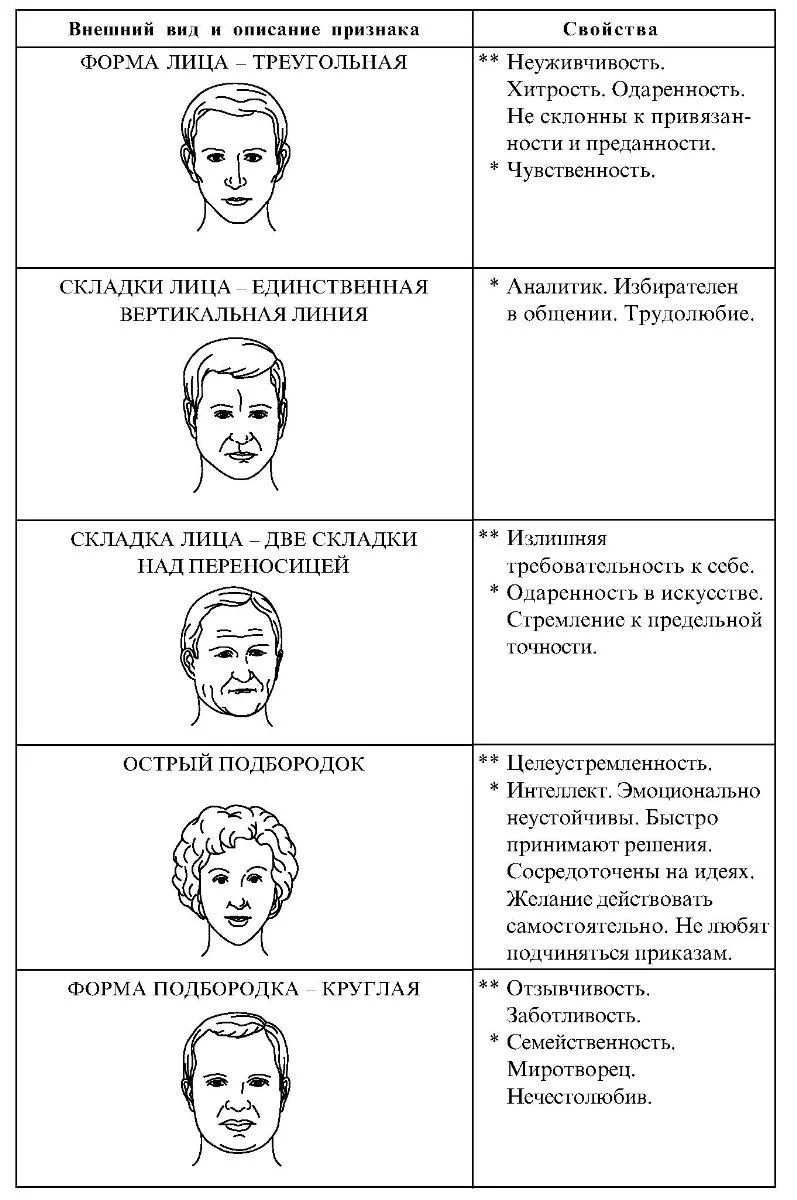
\includegraphics[width=0.6\textwidth]{img/faces.png}
    \caption{Обратите внимание, если оба века выглядят отечными, это тревожный признак: человек устал от жизни или нездоров.}
\end{figure}

\textbf{Читаем особенности характера мужчины по бровям}

Женские брови часто подвергаются косметической коррекции, поэтому по ним трудно судить о чертах характера. А вот мужские могут многое рассказать об обладателе. В первую очередь следует обратить внимание на толщину бровей. Чем она больше, тем упрямее человек. Важен конец брови: тонкий свидетельствует о благородстве, широкий может говорить мужественности и даже жесткости, отличных предпринимательских качествах.

Если бровь заметно длиннее глаза, перед вами человек с гибким умом, а в целом длинные брови говорят о спокойном и несколько консервативном характере. Грубые и короткие брови часто свидетельствуют о влюбчивости и непостоянстве натуры. Также короткие и густые брови бывают о вспыльчивых, агрессивных и самодостаточных людей. Форма бумеранга указывает на изобретательность.

\begin{figure}[h]
    \centering
    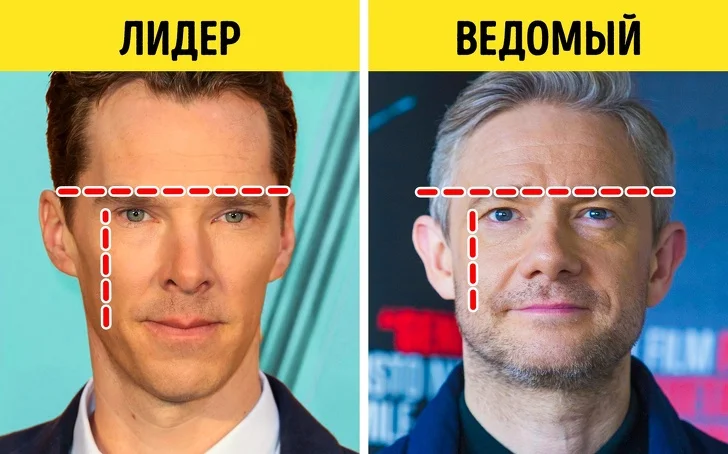
\includegraphics[width=0.5\textwidth]{img/brows.png}
    \caption{Люди, у которых почти отсутствуют брови, закрыты и хитры. Крупные сросшиеся «моноброви» — у решительных, прямолинейных и смекалистых натур. Если внутри брови видна родинка, человек легко добивается целей.}
\end{figure}

\textbf{Правда ли, что длинный нос характерен для лгунов?}

Нет, это сказка. Очень большая длина носа указывает на ум, капризность, а умеренно длинные носы у консервативных людей. Если нос еще широкий, то человек спокоен и устойчив. А короткие носы у дружелюбных открытых оптимистов.

Костлявый нос говорит о плохой концентрации внимания, но если он с горбинкой, то это может указывать на гордый, решительный, упрямый характер, иногда даже агрессивность. Такой нос у женщины свидетельствует, что она конкурентоспособна в мужском коллективе, амбициозна. А маленький нос нередко бывает у ревнивых натур.


\begin{figure}
    \centering
    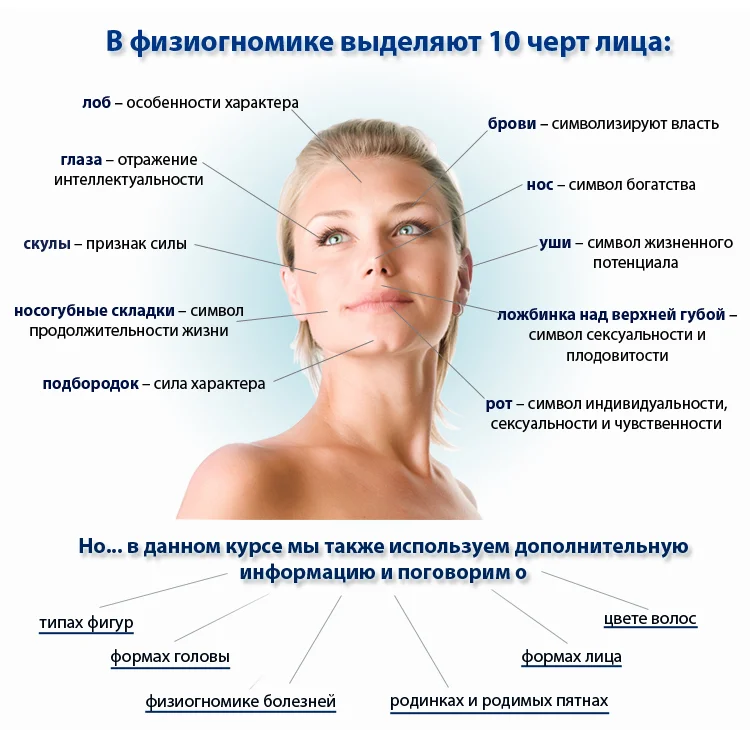
\includegraphics[width=0.65\textwidth]{img/face2.png}
    \caption{В физиогномике выделяют 10 черт лица.}
\end{figure}


Обратите внимание на форму кончика носа:
\begin{enumerate}
    \item Круглая — благополучная натура, умеющая быть счастливой в любых обстоятельствах.
    \item Отвисшая — признак сексуальности.
    \item Заостренная — склонность к непостоянству, предательству.
    \item Выпуклая — свидетельство душевной теплоты.
    \item Похожая на орлиный клюв — мстительность.
    \item Вздернутый нос говорит о сексуальной раскрепощенности, неумении хранить тайны.
\end{enumerate}

Понимание, что означают те или иные особенности носа, дает возможность мгновенно оценить многие свойства характера.

\textbf{Главное о чтении характера человека по внешности}

Помните, что:
\begin{enumerate}
    \item Физиогномика не точная наука, а только учение китайских мудрецов. Не стоит придавать ей излишнего значения.
    \item Современные косметические процедуры творят чудеса. Читая по лицу человека, особенно женщины, легко ошибиться.
    \item Нередки пластические операции. О том, что они вообще были, вы можете узнать только от самого человека.
    \item Черты лица меняются. В зависимости от того, какие мышцы чаще всего задействуются, зависит выражение лица, его особенности. Некоторые черты становятся более выраженными, а какие-то — менее.
\end{enumerate}

Лицо, руки и пальцы многое могут рассказать о человеке, но не следует делать скоропалительных выводов, не пообщавшись с ним.


% \chapter{Личность и характер}

\section{Мой характер}
О себе говорить приятно, но немного трудно. Приятно, потому что всем нравится говорить о своих интересах, вкусах и предпочтениях. Но это в то же время трудно, так как изучить человека, особенно себя самого, не так уж просто.

Прежде чем говорить о своем характере, хотелось бы сначала уточнить, что такое характер. Человек отличается от остальных своими качествами. Часто люди говорят, что я не такой как остальные. Но я не считаю, что я какой-то особенный. В темноте все кошки серые. Но если вы подойдете ближе и включите свет, вы увидите, что мне присущи определенные черты.

Но не будем вдаваться в подробности, и немного сократим рассказ. У меня хорошее чувство юмора, я ответственный, трудолюбивый и эмоциональный человек. Мне нравится творчество, и я ценю эту черту в других людях. Я не люблю ложь и чувствую, когда другие лгут.

Я стараюсь никогда не опаздывать и \explain{терпеть}{to brook} не могу, когда другие не приходят \explain{вовремя}{on time}. Я предпочитаю общаться с умными и вежливыми людьми. \explain{Досадно}{it's annoying}, когда тот, кому ты \explain{доверяешь}{доверять/доверить: to trust}, оказывается \explain{ненадежным}{ненадежный: unreliable} человеком.

Я стараюсь \explain{обращаться}{to treat / обратиться} с другими так, как я хотел бы, чтобы они обращались со мной. Я ищу человека со здоровым и сильным ум\'{о}м и телом. Человека, с которым интересно общаться, которому я могу доверять и на кого можно положиться.

Что касается моих интересов, мне нравится психология в плане общения с людьми, а также способа формирования мыслей наилучшим образом. Я очень люблю путешествовать, встречаться с новыми людьми, знакомиться с их традициями и обычаями, их культурой, смотреть достопримечательности. Мне также нравятся разные стили музыки, нравится ритмичная музыка, под которую можно танцевать.
\chapter{Образование}

\section{Образование}

\textit{Источник: \url{https://bit.ly/3mQJ8N7}}

\textbf{Важность образования.}
Невозможно переоценить важность образования в современном мире. Образование стало ведущей силой технологического прогресса и тем самым всего развития человечества.

\textbf{Виды образования в России.}
В нашей стране есть разные виды образования: дошкольное, начальное, среднее и высшее.
Дошкольное образование охватывает ясли и детские сады. Там за детьми присматривают профессиональные няни и воспитатели. Часто их обучают читать и считать.

В России есть разные виды школ. Все школы начинаются с начального образования. Оно продолжается до 5 класса. Большинство учеников ходят в средние школы, другие идут в лицеи, гимназии, специализированные школы. Если ученики успешно оканчивают среднюю школу, они получают аттестат о среднем образовании. Он дает им возможность поступить в университет или академию, которые являются учреждениями высшего образования.

Учреждения высшего образования сейчас готовят специалистов, магистров и докторов. Диплом о высшем образовании позволяет найти более хорошую работу.

\textbf{Виды образования в других странах.}
В разных странах системы образования различны. В Британии три ступени образования. У Британцев есть начальная школа, средняя школа и высшее образование. Последнее включает профессиональное и собственно высшее образование.
В США система образования очень децентрализована. Это означает, что каждый штат имеет свои законы об образовании. Как правило, там есть начальные школы (6-11 лет), средние школы (11-15 лет) и старшие школы (9-12 классы). Есть несколько способов продолжить образование: университеты, колледжи, местные колледжи, технические и профессиональные школы.


\section[Что мешает хорошо обучаться]{Ученые из России и Швеции выяснили, что мешает хорошо обучаться}

\textit{Источник: \url{https://trends.rbc.ru/trends/education/62a849179a7947b0cc4329a4?from=mainpage}}

Ученые из МГУ, Сколтеха и Стокгольмского университета выяснили, от чего зависит способность к обучению. Рассказываем, что нужно об этом знать

\textbf{Что происходит}

В организме белок синтезируется с помощью рибосом в ядре и цитоплазме, либо в митохондриях. Первый способ изучен хорошо, второй — недостаточно.

Два года назад ученые из МГУ открыли два фермента — белковых соединения, которые участвуют в сборке рибосом в митохондриях. Затем ученые из Стокгольмского университета выделили митохондрии с недостроенными рибосомами, определили их структуру и показали процесс их сборки. Выяснилось, что в этих клетках были неактивными ферменты метилтрансферазы.

Чтобы проверить влияние неактивных ферментов на организм, ученые из МГУ вырастили мышей с такими ферментами. Затем провели эксперимент: посадили животное в ящик с несколькими выходами, где только один ведет в домашнюю клетку, остальные — в тупик. Если нормальная мышь запоминает правильный выход и в следующие разы бежит именно туда, то мышь с неактивными ферментами не запоминает правильный путь и каждый раз ищет его заново.

Таким образом, пришли к следующему выводу. Если ферменты метилтрансфераза неактивны, то работа митохондрий нарушается, и в клетки перестает поступать энергия. Из-за этого мышцы становятся слабее, а интеллектуальные способности снижаются.

\textbf{Что это значит}

Ученые из МГУ уже исследовали нарушения в работе митохондрий. В мае 2022 года они пришли к выводу, что нарушение работы этих органелл приводит к старению. Это происходит из-за того, что с возрастом появляется все больше нарушений в работе митохондрий, и клетки не успевают их устранять. Чтобы уменьшить число поломок и замедлить старение, согласно исследованиям ученых, нужно соблюдать диету.

По словам руководителя отдела разработки ДНК-тестов в компании MyGenetics Валерия Полуновского, чем лучше работают митохондрии в организме человека, тем лучше функционирует тело и мозг. А чтобы число митохондрий в клетках стало больше, нужно заниматься спортом.


% \chapter{Окружающая среда и природа}

\section{Городск\'{а}я жизнь}
Вы никогда не думали о последствиях жизни в городе? Казалось бы, \explain{на первый взгляд}{at first sight}, что жизнь в больших экономических и культурных центрах имеет только преимущества, но дальнейшее рассмотр\'{е}ние показывает, что она имеет и \explain{недостатки}{недостаток: disadvantage}.

С \explain{положительной}{полож\'{и}тельный/-ая: positive} стороны, легче найти работу в городе, потому что там обычно много ресторанов, кафе, гостиниц, школ, библиотек, музеев и т.д. Кроме того, жители города имеют прекрасную возможность посетить множество культурных и развлекательных учреждений, таких как музеи, галереи, ночные клубы, дискотеки и многое другое.

С другой стороны, жителям города \explain{приходится}{приходиться/прийтись: have to} жить в загрязненной атмосфере из-за интенсивного автомобильного движения и \explain{промышленных}{industrial} \explain{предприятий}{предпри\'{я}тие: enterprise}. Это может \explain{вызвать}{to cause} \explain{заболевания}{disease} лёгких и проблемы с сердцем. Кроме того, городской образ жизни довольно \explain{напряженный}{intense}, \explain{поскольку}{since/because} приходится много работать, много ездить на автомобиле и, в результате, стоять в пробках...

В заключение, городская жизнь имеет некоторые преимущества. Тем не менее, она также \explain{может нанести ощутимый вред}{can cause significant damage}, так что местные власти должны сделать несколько важных решений, например, они должны \explain{запретить}{[запрещать] to ban} промышленные предприятия в городах и вблизи городов, которые загрязняют воздух и воду токсичными парами.

\section{Причины и последствия загрязнения окружающей среды}
\textit{Источник: \url{https://bit.ly/3NV3JeZ}}

Загрязнение окружающей среды в настоящее время является самой большой проблемой, с которой сегодня \explain{ст\'{а}лкивается}{faces, is facing} мир. Наприм\'{е}р, в Соединенных Штатах 40\% рек и 46\% озёр слишком загрязнен\'{ы} для рыбной л\'{о}вли, \ed{купания}{купание}{bathing} и водных организмов. Это \explain{неудивительно}{not surprising}, когда ежегодно в американские воды \explain{сбрасывается}{dumped} 1,2 триллиона галлонов \explain{неочищенных}{untreated} ливневых вод, промышленных \ed{отходов}{отх\'{о}ды}{waste} и неочищенных \ed{сточных вод}{ст\'{о}чные в\'{о}ды}{sewage}.

Одна треть верхнего \ed{слоя}{спой}{layer} \ed{почвы}{почва}{soil} в мире уже деградирована, и \explain{с учётом}{taking into account} нынешних темпов деградации почвы, вызванной неправильными методами ведения сельского хозяйства и промышленности, а также \ed{обезлесением}{обезлесение}{deforestation}, большая часть верхнего слоя почвы в мире может исчезнуть в течение следующих 60 лет.

Великий смог 1952 года унёс жизни 8000 человек в Лондоне. Это событие \explain{было вызвано}{was caused (by)} периодом холодной погоды \explain{в сочетании с}{in conjunction with} безветренными условиями, которые сформировали \explain{плотный}{dense} слой переносимых по воздуху загрязнителей, в основном от угольных электростанций, над городом.

Существует множество источников загрязнения, каждый из которых по-своему влияет на окружающую среду и живые организмы. В этой статье обсуждаются проблема загрязнения и последствия различных видов загрязнения.

\textbf{Причины.} Причины загрязнения не \explain{ограничиваются}{are limited} только выбросами \ed{ископаемого топлива}{ископ\'{а}емое т\'{о}пливо}{fossil fuel} и \ed{углерода}{углерод}{carbon}. Существует множество других типов загрязнения, включая химическое загрязнение \ed{водоёмов}{водоём}{reservoir} и п\'{о}чвы в результате неправильной утилизации и сельскохозяйственной деятельности, а также шумов\'{о}е и светов\'{о}е загрязнение, создаваемое городами и урбанизацией в результате роста населения.

\textbf{Загрязнение воздуха.}
Существует два типа \ed{загрязнителей}{загрязн\'{и}тель}{pollutant} воздуха: \ed{первичные}{перв\'{и}чный}{primary} и \ed{вторичные}{вторичный}{secondary}. Первичные загрязнители выбрасываются \explain{непосредственно}{directly} из их источника, в то время как вторичные загрязнители образуются, когда первичные загрязнители вступают в реакцию в атмосфере.

\ed{Сжигание}{сжиг\'{а}ние}{burning, combustion} ископаемого топлива для тр\'{а}нспорта и электричества производит как первичные, так и вторичные загрязнители и является одним из крупнейших источников загрязнения воздуха.

\ed{Выхлопные газы}{выхлопные газы}{traffic fumes; exhaust fumes} автомобилей содержат опасные газы и \explain{твёрдые частицы}{solid particles}, включая \ed{углеводороды}{углеводород}{hydrocarbon}, оксиды азота и монооксид углерода. Эти газы \explain{поднимаются}{rise} в атмосферу и \explain{вступают в реакцию}{react} с другими атмосферными газами, создавая ещё б\'{о}лее токсичные газы.

По данным Института Земли, интенсивное использование \ed{удобрений}{удобрение}{fertiliser} в с\'{е}льском хоз\'{я}йстве является основным источником загрязнения воздуха \ed{мелкими частицами}{мелкие частицы}{microparticles}, что \explain{затронуло}{affected} большую часть Европы, России, Китая и США. Считается, что уровень загрязнения, вызванного сельскохозяйственной деятельностью, \explain{превышает}{exceeds} все другие источники загрязнения воздуха мелкими частицами в этих странах.

\ed{Аммиак}{амми\'{а}к}{ammonia} -- это основной загрязнитель воздуха, \explain{образующийся}{emerging} в результате сельскохозяйственной деятельности. Аммиак попадает в воздух в виде газа из концентрированных отходов животноводства и полей, которые \explain{чрезм\'{е}рно}{excessively} уд\'{о}брены.

Затем этот \explain{газообразный}{gaseous} аммиак соединяется с другими загрязнителями, такими как оксиды и сульфаты азота, образующиеся в транспортных средствах и промышленных процессах, с образованием аэрозолей. Аэрозоли -- это \explain{крошечные}{tiny} частицы, которые могут \explain{проникать}{permeate} глубоко в лёгкие и вызывать сердечные и лёгочные заболевания.

Другие сельскохозяйственные загрязнители воздуха включают пестициды, \explain{гербициды}{herbicides} и фунгициды. Все это также способствует загрязнению воды.

\textbf{Загрязнение воды.}
Загрязнение \ed{питательными веществами}{пит\'{а}тельные веществ\'{а}}{nutrients} вызывается сточными водами и удобрениями. Выс\'{о}кие уровни питательных веществ в этих источниках попадают в водоемы и способствуют росту \ed{водорослей}{водоросли}{algae} и \ed{сорняков}{сорняк}{weed}, что может сделать воду \ed{непригодной}{непригодный}{unusable; unfit} для \ed{питья}{питьё}{drinking} и \explain{истощить}{deplete} кислород, что \explain{приведет к гибели}{will lead to death} водных организмов.

Пестициды и гербициды, \explain{применяемые}{used; applied} для сельскохозяйственных культур и жил\'{ы}х районов, концентрируются в почве и перен\'{о}сятся в грунтовые воды с дождевой водой и стоками. По этим причинам каждый раз, когда кто-то пробуривает \ed{скважину}{скважина}{well (water well)} на воду, её необходимо проверять на \explain{наличие}{availability} загрязняющих веществ.

Промышленные отходы являются одной из основных причин загрязнения воды, поскольку они создают первичные и вторичные загрязнители, включая \ed{серу}{сера}{sulfur}, \explain{свинец}{lead} и \explain{ртуть}{mercury}, нитраты и фосфаты, а также разливы нефти.

В \ed{развивающихся странах}{развив\'{а}ющиеся стр\'{а}ны}{developing countries} около 70\% \explain{твёрдых отходов}{solid waste} сбрасывается непосредственно в океан или море. Это вызывает серьёзные проблемы, включая причинение вреда и убийство \ed{морских существ}{морские существа}{sea creatures}, что \explain{в конечном итоге}{eventually} влияет на людей.

\textbf{Загрязнение земли и п\'{о}чвы.}
Загрязнение земель -- это разрушение зем\'{е}ль в результате деятельности человека и неправильного использования земельных ресурсов. Это происходит, когда люди наносят на почву химические вещества, такие как пестициды и гербициды, неправильно утилизируют отходы и \explain{безответственно}{irresponsibly} \explain{эксплуатируют}{exploit} полезные ископаемые при \ed{добыче}{добыча}{mining} полезных ископаемых.

Почва также загрязняется из-за протекающих подземных септиков, канализационных систем, вымывания вредных веществ со \ed{свалок}{свалка}{landfill} и прям\'{о}го сбр\'{о}са сточных вод промышленными \ed{предприятиями}{предприятие}{enterprise} в реки и океаны.

Дождь и наводнение могут переносить загрязнители с других уже загрязнённых зем\'{е}ль в п\'{о}чву в других местах.

Избыточное \explain{земледелие}{agriculture} и чрезм\'{е}рный \explain{в\'{ы}пас}{grazing} в результате сельскохозяйственной деятельности прив\'{о}дят к тому, что п\'{о}чва теряет свою питательную ценность и структуру, вызывая деградацию почвы, ещё один тип загрязнения почвы.

Свалки могут вымывать вредные вещества в почву и водные пути и создавать очень неприятные запахи, а также являются рассадниками \ed{грызун\'{о}в}{грыз\'{у}н}{rodent}, которые являются переносчиками болезней.

\textbf{Шум и световое загрязнение.}
Шум считается загрязнителем окружающей среды, вызываемым бытовыми источниками, общественными мероприятиями, коммерческой и промышленной деятельностью и транспортом.

Световое загрязнение вызвано длительным и чрезмерным использованием искусственного \ed{освещения}{освещение}{lighting} в ночное время, что может вызвать проблемы со здоровьем у людей и нарушить естественные циклы, \explain{в том числе}{including} деятельность \explain{дикой}{wild} природы. Источники светового загрязнения включают электронные рекламные щиты, ночн\'{ы}е спортивные площадки, уличные и автомобильные фонар\'{и}, городск\'{и}е парки, общественные места, аэроп\'{о}рты и жил\'{ы}е районы.


\chapter{Наука и Техника}


\section{Компьютер}
\textbf{Компьютер и его история.} Компьютеры появились в жизни людей не так давн\'{о}. В середине 20 века простые люди не имели понятия о них. В 1951 году был внедрён первый \explain{коммерчески доступный}{commercially available} компьютер. В 1975 году появились персональные компьютеры.

\textbf{Важность компьютеров.} Трудно представить современную жизнь без компьютеров. Сфера их \explainDetail{применения}{применение}{application} очень широк\'{а}.
Большинство офисов оснащен\'{о} компьютерами для вычислений и работы с документацией. Ранее недоступные хирургические операции сегодня выполняются благодаря компьютерным технологиям. Технологии также внедрены в современном образовании, ими пользуются как студенты, так и преподаватели.

\textbf{Роль компьютеров в жизни подростков.}
Они используют компьютеры для различных целей. Во-первых, играют в компьютерные игры, смотрят мультфильмы и фильмы. Во-вторых, делают школьные задания, читают книги и находят различную информацию в интернете.

\explainDetail{Сравн\'{и}тельно}{сравн\'{и}тельно}{relatively} новая тенденция --- общение онлайн. Такие \explainDetail{приложения}{приложение}{computer application}, как Skype, позволяют в режиме реального времени общаться с людьми, которые находятся очень далеко.

\textbf{Угрозы, связанные с компьютерами.}
Компьютеры оказывают не только положительное влияние на детей. Одна из \explainDetail{угроз}{угр\'{о}за}{threat} --- \explain{вовлечение}{involvement} в виртуальную реальность. Некоторые дети так много времени пров\'{о}дят за компьютером, что забывают о реальных л\'{ю}дях вокруг них.

В результате они будут лишены важных социальных \explainDetail{н\'{а}выков}{н\'{а}вык}{skill} в будущем. Сидя за компьютером, дети портят глаза и осанку. Поэтому взрослые должны быть очень внимательны к тому, как долго их дети пользуются компьютерами.




\section{Северное сияние}
С \explainDetail{наступлением}{наступление}{adventб beginning} осени тысячи туристов \explain{устремляются}{rush} в \explain{Заполярье}{the region of the Arctic circle}, чтобы увидеть уникальный танец небесных огней -- полярное, или северное сияние, на латыни -- Aurora Borealis.
В теории увидеть это природное явление можно с конца августа до середины апреля: в этот период времени ночи становятся темными, солнечная активность \explainDetail{возрастает}{возрастать/возрасти}{возраст\'{а}ю/-ешь/-ет; возраст\'{у}/-ёшь/-\'{у}т: rise, increase}, а облака \explainDetail{расс\'{е}иваются}{рассеиваться/рассеяться}{to disperse}.
Такое развлечение, как \explain{ох\'{о}та}{hunting} за северным сиянием, с каждым годом становится все популярнее как среди россиян, так и среди иностранных туристов, которые специально ради него готовы ехать на Крайний Север. Главное \explain{доказательство}{proof} удачной охоты -- это, конечно же, снимки северного сияния.


\section{Только дьявол мог выдумать Нобелевскую премию}
% https://www.gazeta.ru/science/2015/11/27_a_7914947.shtml
Екатерина Шутова

\textit{120 лет назад Альфред Нобель подписал \explain{завещ\'{а}ние}{will} по Нобелевской премии.}

120 лет назад Альфред Нобель подписал завещание, согласно которому его \explain{накопл\'{е}ния}{accumulation} поступили в фонд Нобелевской премии -- самой престижной на сегодняшний день \explainDetail{награды}{нагр\'{а}да}{prize}, ежегодно \explainDetail{присуждаемой}{присужд\'{а}емый}{awarded} за выдающиеся научные исследования, революционные изобретения или крупный \explain{вклад}{contribution} в культуру или развитие общества. \explainDetail{Отдел}{отдел}{department} науки «Газеты.Ru» вспоминает \explainDetail{подробности}{подробность}{detail} этого события.

В 1888 году журналисты \explain{оповестили}{notified} мир о смерти Альфреда Нобеля -- химика, инженера и изобретателя динамита. Репортеры ошиблись -- на самом деле погиб Людвиг Нобель, брат Альфреда.

\begin{fancyquotes}
    Удивленный изобретатель прочитал в одной из газет собственный некролог под названием «Торговец смертью мертв».
\end{fancyquotes}

Альфред Нобель не захотел оставаться злодеем в глазах человечества. Поэтому 27 ноября 1895 года в Шведско-Норвежском клубе в Париже ученый составил следующее завещание:

{\it
Я, \explain{нижеподписавшийся}{undersigned}, Альфред Бернхард Нобель, обдумав и решив, настоящим объявляю мое завещание по поводу имущества, нажитого мною... Капитал мои душеприказчики должны перевести в ценные бумаги, создав фонд, проценты с которого будут выдаваться в виде премии тем, кто в течение предшествующего года принес наибольшую пользу человечеству.

Указанные проценты следует разделить на пять равных частей, которые предназначаются: первая часть тому, кто сделал наиболее важное открытие или изобретение в области физики, вторая --- в области химии, третья --- в области физиологии или медицины, четвертая --- создавшему наиболее значительное литературное произведение, отражающее человеческие идеалы, пятая --- тому, кто внесет весомый вклад в сплочение народов, уничтожение рабства, снижение численности существующих армий и содействие мирной договоренности.

... Мое особое желание заключается в том, чтобы на \explain{присуждение}{awarding, conferment} премий не \explainDetail{влияла}{влиять/повлиять}{influence} национальность кандидата, чтобы премию получали наиболее \explain{достойные}{worthy}, независимо от того, скандинавы они или нет.}

\subsection{Как огорчить родственников}
Спустя год после написания завещания Альфред Нобель скончался на своей вилле от \explainDetail{кровоизлияния}{кровоизлияние}{hemorrhage} в мозг. За несколько лет до смерти ученый сказал о самом себе следующим образом: «Альфред Нобель -- его \explain{существование}{existence} следовало бы \explain{пресечь}{suppress} при рождении милосердным доктором. Основные добродетели: держит ногти в чистоте и никому не бывает в тягость. Основные недостатки: не имеет семьи, наделен дурным характером и плохим пищеварением.

\begin{fancyquotes}
    Величайший грех: не поклоняется Мамоне. Важнейшие события в его жизни: никаких.
\end{fancyquotes}

\explain{Наследники}{heirs} легендарного изобретателя были крайне \explain{возмущены}{outraged}, что огромные накопления уйдут не им в карман, а на поддержку науки. Они требовали, чтобы завещание было признано недействительным. Интересно, что единственным родственником Нобеля, не пытавшимся присвоить себе деньги, оказался его племянник Эммануил. «Русские называют исполнителя завещания «душеприказчик», то есть «представитель души», --- заявил юристам мужчина. --- Вот и действуйте соответственно». Позднее Эммануил добавил: «Я не хочу, чтобы достойнейшие ученые в будущем упрекали нашу семью в присвоении средств, которые по праву принадлежат им».

В конечном итоге справедливость восторжествовала --- и через несколько лет после смерти ученого были вручены пять первых премий. А с 1969 года по инициативе Шведского банка начала присуждаться Нобелевская премия по экономике.

Лишь однажды деньги из фонда премии пошли на дело, никак не связанное с наукой. Софи фон Капивара, женщина, с которой у талантливого изобретателя были отношения, пообещала раскрыть содержание их переписки и посмертно опозорить Альфреда Нобеля. Душеприказчики в страхе выплатили крупную сумму за 216 писем мецената. Ученые до сих пор шутят, что

\begin{fancyquotes}
    наука была бы богаче, если бы не одна алчная молочница.
\end{fancyquotes}

«Ты славная девушка, но ты действуешь мне на нервы»

Существует миф, согласно которому у Альфреда Нобеля была жена, страстно влюбившаяся в математика, и именно поэтому изобретатель «обделил» всех представителей этой науки. Но на самом деле, как заявляют биографы, меценат никогда не был женат. В молодом возрасте Нобель влюбился в работницу аптеки, но та умерла от чахотки. Потосковав, ученый нашел новую пассию --- на этот раз ей стала Сара Бернар, знаменитая актриса. Альфред Нобель написал письмо матери о том, что хочет жениться.

\begin{fancyquotes}
    Недаром актеров в старину не разрешали хоронить на кладбище. У них нет души, сыночек!» --- предупредила сына любящая родительница.
\end{fancyquotes}



Послушный Нобель разорвал любовную связь с Бернар.

Следующая женщина появилась в жизни мецената, когда тому уже был 41 год. Альфред Нобель опубликовал в газете объявление о том, что ищет секретаршу. На него откликнулась графиня Берта Кински, с которой у изобретателя начался неторопливый и гармоничный роман.

\begin{fancyquotes}
    Кстати, по одной из версий, именно Кински попросила Нобеля вписать в завещание премию мира. А в 1905 году она стала первой женщиной, удостоенной этой премии.
\end{fancyquotes}

У Кински и Нобеля дело до свадьбы не дошло: однажды ученый обнаружил, что его секретарша исчезла, оставив на столе письмо следующего содержания: «Простите меня, господин Нобель. Я уезжаю в Вену, где меня ждет жених. Пожелайте мне счастья, как я желаю счастья вам. Искренне преданная вам Берта Кински, которая в скором времени станет Бертой фон Зуттер».

Последней женщиной в жизни Нобеля стала вышеупомянутая «алчная молочница», которая изрядно надоедала ученому своей глупостью и необразованностью. «Дорогое дитя. Ты славная девушка, но ты действуешь мне на нервы», --- раздраженно писал ей в письмах Альфред Нобель.

Так почему же не существует премии по математике? Возможно, все дело в том, что у Альфреда Нобеля не заладились отношения с великим математиком Миттаг-Леффлером, который должен был стать первым лауреатом, а меценат этого не хотел. Но наиболее вероятная версия заключается в том, что Нобель воспринимал математику как инструмент, как сугубо теоретическую науку.

\subsection{Виагра для хомячков и исследование ругани}

В 1991 году появилась пародия на Нобелевскую премию --- Шнобелевская премия. Она вручается «за достижения, которые заставляют сначала засмеяться, а потом --- задуматься». Учредитель и идейный вдохновитель «Шнобелевки» --- Марк Абрахамс, который, будучи редактором юмористического научного журнала, получал множество писем от читателей с подробным рассказом об их «великих» исследованиях. «Иногда эти люди заслуживали премии --- правда, не Нобелевской», --- говорил Абрахамс. Так редактор решил награждать ученых за самые нелепые достижения.

В разные годы Шнобелевская премия присуждалась

за разработку протезов яичек для собак, за исследование влияния музыки кантри на частоту самоубийств и за открытие, что «Виагра» помогает хомякам справиться с последствиями резкой смены часовых поясов.

Также пародийную награду получали ученые, доказавшие, что ругань снижает боль, и исследователи, изучавшие оральный секс у летучих мышей.

Первым в мире человеком, удостоенным как Шнобелевской, так и Нобелевской премии, стал Андрей Гейм. Голландский ученый российского происхождения был награжден «Шнобелевкой» за использование магнитов для того, чтобы демонстрировать возможность левитации лягушек. Спустя десять лет Гейм совместно со своим учеником Константином Новоселовым получил Нобелевскую премию за изобретение графена.

\subsection{Война еще не закончена, а премии уже раздают}
«Я готов простить Альфреду Нобелю изобретение динамита, но только дьявол в людском обличье мог выдумать Нобелевскую премию!» --- воскликнул ирландский романист и драматург Джордж Бернард Шоу, став лауреатом в области литературы (по ироничному заявлению писателя, произошло это потому, что «в тот год он ничего не опубликовал»). Действительно, самая престижная международная награда --- явление весьма резонансное и неоднозначное. В Советском Союзе Нобелевский комитет клеймили за то, что «он ухитрился не заметить Алексея Толстого, Максима Горького, Владимира Маяковского, но зато заметил Ивана Бунина. И только тогда, когда он стал эмигрантом, и только потому, что он стал эмигрантом и врагом советского народа».

В Третьем рейхе ученым было запрещено получать Нобелевскую премию, так как в 1935 году премию мира «За борьбу с милитаризмом в Германии» получил пацифист Карл фон Осецкий --- ярый противник нацистского режима. В 1937 году Адольф Гитлер издал указ, согласно которому немцы не имели права принимать премию. Из-за указа награду не получили Герхард Домагк «за открытие антибактериального эффекта пронтозила», Адольф Бутенандт за исследование половых гормонов и Рихард Кун за работу по каротиноидам и витаминам.


\begin{fancyquotes}
    Весьма примечателен тот факт, что Бенито Муссолини и Адольф Гитлер были номинированы на Нобелевскую премию мира в 1935 и 1939 годах соответственно.
\end{fancyquotes}

Нобелевская история знает немало случаев отказа от самой престижной международной награды.

Так, в 1973 году политический деятель Фан Динь Кхай отказался от медали «за работу по разрешению вьетнамского конфликта», аргументируя свое решение тем, что «война еще не закончена, а премии уже раздают». Не захотел быть награжденным и Жан-Поль Сартр --- французский писатель и драматург. По мнению Сартра, награда посягнет на его независимость --- центральное понятие в философии автора. Вскоре после отказа от Нобелевской премии француз еще раз шокировал общественность, заявив, что уходит из литературы. «Литература --- суррогат действенного преобразования мира», --- с горечью заметил писатель.

\section{Ученые нашли способ записать данные в пяти измерениях}

\textit{Как 5D-диски изменят представление людей о хранении информации?}

\textbf{Ученые создали 5D-диск высочайшей плотности:} В октябре специалисты Саутгемптонского университета в Великобритании описали способ записи огромного количества данных на компактный диск небольших размеров. Технология, получившая название 5D, позволяет сохранить на специальном накопителе до 500 терабайт информации. Получившиеся диски из кварцевого стекла отличаются высочайшей плотностью, которая в десять тысяч раз превышает плотность оптических дисков Blu-Ray. Новый метод позволит эффективно разместить на небольшой площади облачные сервера для хранения данных пользователей, интернет-компаний, крупных корпораций. По словам ученых, это особенно важно на фоне развития технологий, увеличения количества подключенных к сети устройств и роста количества передаваемых через сеть данных.

\textbf{Облачные сервисы с каждым годом становятся все популярнее:}
За последние пять лет отношение потребителей и бизнеса к облачным сервисам изменилось. Раньше их воспринимали в качестве дополнительного метода резервного копирования данных --- информация практически всегда поступала в одну сторону. Причем крупные корпорации в основном использовали дата-центры для хранения некритичной информации. К 2020-м годам организации стали использовать облачные серверы не только для аварийного копирования, но и для постоянного обмена данными внутри конкретного предприятия. Системы облачных хранилищ стали более гибкими, позволяя конкретному потребителю выбрать необходимое количество свободного места и производительность оборудования.

Специалисты Analytics Insight называют основными \explainDetail{преим\'{у}ществами}{преим\'{у}щество}{advantage} \explainDetail{облачных}{облачный}{cloud (adj.); \'{о}блако: cloud} дата-центров \explain{круглос\'{у}точный}{round the clock} доступ к информации, возможность одновременной работы не- скольких пользователей с одним массивом данных, масштабируемость и \explain{г\'{и}бкость}{flexibility}, \explain{снижение}{decline} затрат на хранение данных внутри компании.

\explainDetail{Представители}{представитель}{representative} отрасли отмечают, что в обычное время нагрузка на серверы неравномерна: в одной части дата-центров она может зашкаливать, в другой быть крайне небольшой. По этой причине эксперты предсказывают появление искусственного интеллекта, который мог бы анализировать и распределять нагрузку на оборудование. В том числе по этой причине данные пользователей хранятся в нескольких частях дата-центра.

\textbf{Больше всего в облачных сервисах пользователи ценят скорость передачи данных и безопасность:} По словам основателя облачного провайдера Wasabi Дэйва Френда, от дата-центров будущего потребители ожидают высокого уровня безопасности, производительности оборудования и приемлемой цены за услуги. «Резервные копии должны храниться в разрозненных системах, обеспечивающих максимально возможную изоляцию», --- заметил предприниматель. Потенциальный злоумышленник, добравшийся до одного сервера, не должен иметь возможность удалить или зашифровать информацию так, чтобы ее нельзя было восстановить из альтернативных источников. Френд полагает, что на этом должна строиться концепция мультиоблака.

Другими критериями облачного сервиса будущего, по мнению Френда, являются доступная цена и высокая скорость передачи данных. Провайдеры должны будут таким образом скорректировать стоимость услуг и добиться определенного качества оборудования, чтобы оставаться конкурентоспособными и не разочаровывать клиентов.

Представители облачного провайдера CloudSigma рассказали, что дата-центры должны будут отвечать за сохранность данных и скорость передачи информации. Для хранения файлов пользователей и корпоративных клиентов они используют небольшие 2,5-дюймовые диски емкостью 250 гигабайт. В случае, если какой-либо диск выходит из строя, его заменяют, а данные восстанавливают через бэкап. При таком развитии событий клиент не теряет своих данных, хотя и оказывается без доступа к информации на 10-15 минут. Благодаря глубокой интеграции между серверами и оборудованием задержка передачи данных внутри дата-центра очень мала. Для того чтобы разогнать скорость и снизить задержку между серверами и пользователем, в компании полагаются на выделенную гигабитную линию интернета.


\textbf{Диски 5D позволят хранить информацию практически бесконечно:}
По оценке Forbes, к 2025 году к интернету будет подключено около 80 миллиардов устройств, которые будут генерировать около 180 триллионов гигабайт данных. В обозримом будущем хранить данные на классических накопителях будет проблематично --- существует риск возникновения дефицита и увеличения стоимости хранения информации. Работающие над технологией 5D специалисты Саутгемптонского университета предлагают записывать информацию на кварцевом стекле с помощью фемтосекундных лазеров и сверхкоротких импульсов. «Запись на кварцевый носитель как бы идет в пяти измерениях --- двух оптических и трех пространственных», --- отмечают авторы исследования.

Инновация британских инженеров заключается в создании дисков повышенной плотности и размещении на небольшом участке колоссальных объемов данных. Например, на «болванке» размером в один дюйм удалось сохранить шесть гигабайт информации. Накопитель обычного для подобных устройств размера, основанный на кварцевых дисках, может сохранить до 500 терабайт данных. Разработка обещает революцию на рынке хранения информации, так как десятки, если не сотни классических дата-центров можно будет объединить в одну библиотеку.

Преимуществами 5D-дисков также называют долговечность и низкую стоимость обслуживания. По оценке ученых, кварцевые диски не прочнее обычных накопителей, однако могут выдержать температуру до 1800 градусов по Фаренгейту, или около тысячи градусов по Цельсию. В случае пожара в дата-центре информация, скорее всего, сохранится. Кроме того, кварцевое стекло со временем не меняет своих свойств, что позволит держать данные на 5D-накопителях практически вечно.

Единственным узким местом будущей разработки является скорость передачи данных. В настоящий момент ученым удалось разогнать ее до 230 килобайт в секунду --- за это время на диск можно записать около ста страниц текста. Однако для того, чтобы полностью заполнить болванку емкостью 500 терабайт, потребуется 60 дней. Либо инженеры найдут способ обойти ограничение, либо 5D-диски так и останутся перспективным оборудованием для записи информации. В крайнем случае на подобных дисках можно сохранять данные для потомков. Так, в 2018 году на кварцевый носитель была записана трилогия романов Айзека Азимова «Основание» --- диск отправился в космос вместе с Tesla Roadster Илона Маска.



\section{У коронавируса есть механизм самоуничтожения}
% https://russian.rt.com/science/article/937351-pyotr-chumakov-intervyu-virusy
\textit{Пётр Чумаков об эволюции SARS-CoV-2 и лечении вирусами}

\explainDetail{Снижение}{снижение}{decrease} патогенности новых \explainDetail{штаммов}{штамм}{strain (of virus)} SARS-CoV-2 \explain{предопределено}{predetermined} самой логикой эволюции вирусов такого типа. Об этом в интервью RT рассказал член-корреспондент \explain{РАН}{Российская академия наук}, профессор и главный научный сотрудник Института молекулярной биологии РАН Пётр Чумаков. Он также отметил, что многие вирусы можно поставить на службу человеку: например, использовать их непатогенные варианты для защиты людей от опасных \explainDetail{возбудителей}{возбудитель}{pathogen}. За вакцинами, основанными на этом принципе, будущее, считает учёный. По его мнению, вирусы можно использовать и для лечения рака.

{\bf --- С самог\'{о} \explain{начала}{from начало (\textit{суш.}): start, beginning} пандемии многие боялись появления \explain{ос\'{о}бо}{especially, particularly} \explainDetail{смертоносного}{смертоносный}{deadly} штамма вируса. Почему этого пока не случилось? По \explainDetail{предварительной}{предварительный}{preliminary} информации, новый штамм «омикрон» не привёл к \explainDetail{резкому}{резкий}{sharp} росту \explainDetail{летальности}{летальность}{lethality}. Да и в целом опасные мутации \explainDetail{распространённых}{распространённый}{widespread} вирусов случаются не очень часто --- например, даже грипп вызвал смертельную пандемию только один раз, в начале XX века.}

--- Коронавирус SARS-CoV-2 --- новая для человека инфекция. Она перешла в человеческую популяцию только два года назад. До этого коронавирус этого типа циркулировал в основном среди \explainDetail{летучих мышей}{летучая мышь}{bat}. Эти животные \explainDetail{обладают}{обладать}{possess} очень сильной противовирусной защитой, организм летучих мышей заточен для противостояния инфекциям, поскольку они живут в очень \explainDetail{скученных}{скученный}{crowded} колониях. Вирусы, которые способны \explain{пробить}{pierce} эту защиту, должны также быть \explain{вооружены}{armed} очень серьёзными системами преодоления противовирусного иммунитета. И когда такой вирус попадает к человеку, он вызывает тяжёлые \explainDetail{заболевания}{заболевание}{disease}, потому что человеческая иммунная противовирусная система слабее, чем у летучих мышей.

Однако, попав в организм человека, такой вирус тоже должен \explain{приспособиться}{adapt} к новым условиям. Поэтому первые фазы эволюции вируса --- это \explain{накопление}{accumulation} таких мутаций, которые будут приводить к его более эффективному \explainDetail{размножению}{размножение}{reproduction} в организме человека. Это \explain{сопровождается}{is accompanied by} ростом инфекционности и усилением патогенных \explainDetail{свойств}{свойство}{property}. Когда вирус активно размножается, он приспосабливается к организму человека и действует более эффективно.

Вторая фаза эволюции вируса --- аттенуирование. Это приспособление вируса к организму при \explainDetail{ослаблении}{ослабление}{weakening} его патогенности.

При этом инфекционность может расти, потому что вирусу важно быстро \explainDetail{распространяться}{распространяться/распространиться}{spread} на новом хозяине. Однако \explain{излишняя}{superfluous, excessive} патогенность ему не нужна. Дело не в том, что вирус \explain{якобы}{ostensibly} знает, что ему невыгодно убивать человека. Нет, просто это качество --- патогенность --- не востребовано в организме человека и поэтому постепенно ослабевает при накоплении мутаций. В результате вирус вызывает всё меньше летальных исходов и тяжёлых случаев.

\begin{fancyquotes}
    Сейчас штамм коронавируса «омикрон» является примером второй фазы эволюции вируса, \explain{наблюдается}{is observed} его аттенуирование при одновременном увеличении \explain{заразности}{infectiousness}. Итогом должно стать превращение коронавируса в обычное сезонное вирусное заболевание.
\end{fancyquotes}

В случае с «омикроном» примечательна внезапность его появления, он сразу накопил 32 мутации по сравнению с предыдущим штаммом. В Африке очень много иммунодефицитных людей, и, по всей видимости, новый штамм \explainDetail{возник}{возникать/возникнуть}{arise (возн\'{и}к, возн\'{и}кла, возн\'{и}кло, возн\'{и}кли)} в организме именно такого человека. В его организме он прошёл тот путь эволюции, который обычно вирус проходит через большую \explainDetail{цепочку}{цепочка}{chain} \explainDetail{заражений}{заражение}{infection}. В итоге в ускоренном режиме этот вирус превратился в менее патогенный вариант.

Впр\'{о}чем, я бы не хотел никого \explainDetail{расхолаживать}{расхолаживать/расхолодить}{discourage}, говоря о том, что бояться нечего. Нет. Пока что это --- лишь оптимистичный сценарий. Мы пока не имеем достаточного числа случаев заболевания этим штаммом, чтобы заявлять о его низкой опасности. Да, по предварительным данным, пока что от него никто не умер. Но нужно понаблюдать за тем, как будет развиваться ситуация, и продолжать вакцинироваться. Потому что даже если оптимистичный сценарий верный, нельзя исключать, что штамм «омикрон» неожиданно исчезнет, как исчез в Японии штамм «дельта».

\explainDetail{По видимости}{по видимости}{apparently}, у коронавируса есть механизм самоуничтожения. Это может случиться и со штаммом «омикрон», а ему на смену придут более \explain{болезнетворные}{pathogenic} варианты.

{\bf --- Как вакцинация \explainDetail{влияет}{влиять/повлиять}{influence} на мутации вируса --- насколько она снижает их вероятность, \explain{учитывая}{considering, taking into account}, что вакцинированные тоже болеют, пусть и в лёгкой форме?}

--- \explainDetail{Особенность}{особенность}{peculiarity} этого коронавируса в том, что даже очень иммунные люди, которые перенесли заболевание или вакцинированы, могут заразиться \explain{повт\'{о}рно}{repeatedly}, даже не чувствуя при этом симптомов. При этом вирус будет выделяться из носоглотки. Однако вероятность мутаций вируса в такой ситуации всё же не очень велика. Гораздо чаще новые варианты вируса возникают в организмах больных людей, особенно иммунодефицитных.

{\bf --- Вы \explainDetail{упомян\'{у}ли}{упомин\'{а}ть/упомян\'{у}ть}{to mention, to refer} феномен \explainDetail{исчезновения}{исчезнов\'{е}ние}{disappearance} «дельты» в Японии. Не могли бы рассказать об этом \explain{подробней}{in more detail (detail: подробность)}? Случалось ли подобное когда-то раньше?}

--- Нет, это новая гипотеза одного из японских исследователей. Гипотеза, на первый взгляд, экстравагантная. Потому что обычно эволюция идёт таким путём, что \explain{выживает}{survives} сильнейший --- наиболее \explain{жизнеспособный}{viable}. А в этом случае произошло, напротив, эволюционное самозатухание вируса. Согласно гипотезе, это связано с мутацией в гене NSP-14. Это один из неструктурных \explainDetail{белков}{бел\'{о}к}{protein} коронавируса, не входящий в состав вирусной \explainDetail{част\'{и}цы}{част\'{и}ца}{particle}. Он нужен для поддержания репликации вируса, корректирует правильность считывания генома, исправляет ошибки. Если этот белок не функционирует, то вирус начинает с большой \explainDetail{скоростью}{скорость}{speed} накапливать мутации, включая летальные. Они приводят к тому, что вирус уже не может размножаться.

Не знаю, \explain{подтвердится}{confirmed} ли эта гипотеза, однако, когда в Японии секвенировали варианты коронавируса до того, как он исчез, оказалось, что там действительно были мутации белка NSP-14.

Более того, предыдущая \explain{вспышка}{outbreak} SARS-1 в 2003 году тоже \explain{затухла}{faded} сама по себе, её даже не успели подавить вакциной.

Что касается «омикрона», я пока не видел никаких данных о том, что у него \explain{повреждён}{damaged} белок NSP-14. Однако этого нельзя исключать, это объяснило бы скорость накопления в нём мутаций.

{\bf --- Ещё говорят, что штамм «омикрон» очень сильно отличается от других штаммов и что в нём нашли элемент генома человека, который также есть в вирусе \explainDetail{простуды}{простуда}{common cold}. И что это делает его менее заметным для иммунной системы.}

--- Нет, что это элемент генома человека --- это ерунд\'{а}. Это маленькая вставка. И когда мы говорим о \explainDetail{посл\'{е}довательности}{посл\'{е}довательность}{sequence}, \explain{допуст\'{и}м}{let's say}, трёх \explainDetail{аминокислот}{аминокислот\'{а}}{aminoacid}, такая посл\'{е}довательность может встречаться и в человеке, и в растении --- \explain{где угодно}{anywhere}.

{\bf --- Нед\'{а}вно вы сказали, что омикрон-штамм может выступить в качестве естественной вакцины. А были такие прецеденты раньше?}

---  Может быть, были, но они не зафиксированы. Однако что такое «живая вакцина»? Это просто вирус, который не имеет высокой патогенности, но \explain{вызыв\'{а}ет}{causes} иммунный ответ. Обычно такой непатогенный штамм делают искусственно. Например, полиомиелитная вакцина была создана путём селекции, были отобраны вирусы, которые \explainDetail{утратили}{утрачивать/утратить}{to lose} способность \explainDetail{поражать}{пораж\'{а}ть/пораз\'{и}ть}{to hit, to affect} нервные \explainDetail{кл\'{е}тки}{кл\'{е}тка}{cell}. При этом они хорошо размножаются в \explainDetail{кишечнике}{кишечник}{intestine} и вызывают \explain{стойкий}{persistent} иммунитет против полиомиелита. Живая вакцина против \explainDetail{кори}{корь}{measles} тоже была создана на основе патогенного вируса кори, который приобрёл свойства непатогенности.

Природа тоже может создавать такие вирусы. И природная аттенуация вирусного штамма --- это, \explain{по с\'{у}ти}{in fact}, именно такой процесс. Такой вирус \explain{вытесняет}{displaces} патогенные варианты и создаёт иммунную прослойку, которая уже не \explainDetail{позволяет}{позвол\'{я}ть/позв\'{о}лить}{to allow, to permit (also: разреш\'{а}ть/разреш\'{и}ть)} новому патогенному варианту вызвать заболевание.

{\bf --- Ранее в Университете Глазго провели исследование, в результате которого \explain{в\'{ы}яснилось}{it turned out}, что люди очень редко болеют одновременно двумя вирусными заболеваниями. Однако точное объяснение этого тогда найти не удалось. Есть ли сейчас какие-то гипотезы на этот счёт? И можно ли использовать «конкуренцию» вирусов в полезных целях, существуют ли подобные проекты?}

--- Да, есть такое правило, хотя из него тоже бывают исключения. В основе этого явления лежит феномен интерференции. Когда человек или животное \explain{заражается}{gets infected (+\textit{твор.})} вирусом, в ответ в организме \explain{выраб\'{а}тывается}{produced} интерферон --- противовирусный бел\'{о}к. Он циркулирует по всем\'{у} организму, клетки в ответ вырабатывают противовирусное состояние. И другому вирусу будет уже очень трудно внедриться в организм в это время. Однако некоторые вирусы вырабатывают противодействие интерфероновому механизму --- тогда возможна сочетанная инфекция. Возможно также одновременное заражение двумя вирусами, когда первый вирус ещё не вызвал противовирусное состояние.

{\bf --- А учёные думали над тем, чтобы как-то использовать этот интерфероновый механизм для борьбы с болезнями?}

--- Конечно. Такие исследования проводились в 1970-е годы, я принимал в них участие. Есть целый ряд непатогенных вирусов, которые обычно \explain{обитают}{inhabit} в кишечнике здоровых детей в возрасте от двух до пяти лет. Их испытывали как средство профилактики сезонных простудных вирусных инфекций. В начале 1970-х годов было проведено \explain{масштабное}{large-scale} испытание более чем на 300 тыс. человек в шести городах СССР. В итоге заболеваемость \explain{ОРВИ}{острая респираторная вирусная инфекция: acute respiratory viral infection} среди привитых снизилась в 3,5 раза. Это очень хороший результат, такой же, как у специфических противовирусных противогриппозных вакцин.

\begin{fancyquotes}
    Примечательно, что профилактика, основанная на механизме интерференции, защищает не только от одного вируса, а от многих. Поэтому такая неспецифическая профилактика очень важна именно в случае появления новых инфекций, чтобы выиграть время до создания специфической вакцины.
\end{fancyquotes}

Тем более что такие препараты применяются в виде \explain{капель}{drops}, \explain{перорально}{orally}. Это не будет вызывать такого \explainDetail{отторжения}{отторжение}{rejections} у антиваксеров.

{\bf --- А сейчас разрабатываются новые препараты с этим принципом действия?}

--- У нас есть панель таких вирусов. Но проблема в том, что такие вещи с большим трудом пробивают себе дорогу. Например, нам не удалось \explainDetail{убед\'{и}ть}{убеждать/убедить}{to convince [убеждать: убеждаю, убеждаешь, убеждают]} использовать этот метод во время \explain{нынешней}{current} пандемии. Потому что наш подход очень дешёвый, он не очень интересен для бизнеса. Ведь на выпуск вакцин выделяются большие деньги.

Но я уверен, что мы вступаем в такое время, когда вирусы могут использоваться и в качестве оружия. Поэтому нужно иметь стратегический \explain{зап\'{а}с}{stock, reserve} \explain{экстренных}{emergency} средств защиты. И надеюсь, что в итоге собранный нами запас непатогенных вирусов будет использован и признан в качестве такого средства.

{\bf --- Раз вирусы могут \explain{конкурировать}{compete} и вытеснять друг друга, не рассматривается ли научным сообществом, к примеру, идея создать генно-инженерными методами не опасный, но очень контагиозный штамм SARS-CoV-2, чтобы вытеснить те его штаммы, которые приводят к высокой летальности? }

--- Это отличный вопрос. Вообще я считаю, чтобудущее вакцинологии --- это жив\'{ы}е вакцины. Просто сейчас мы идём \explain{проторённым}{well-trodden} путём, создаём традиционные вакцины. Либо это инактивированный вирус, либо какие-то генные инженерные продукты --- на основе других вирусов.

При этом аттенуированные штаммы можно создать из л\'{ю}бого болезнетворного вируса. Зная, какие гены участвуют в патогенезе, можно внести искусственные изменения и сделать из него такой безопасный вирус, который будет тем не менее иммуногенен и будет защищать от инфекции.

Но, к сожалению, пока что этот путь не всеми признаётся, широких работ в этом направлении не ведётся.

{\bf --- В 2020 году в интервью RT вы рассказали о \explainDetail{разработке}{разработка}{development} модифицированных вирусов, которые вызывают \explain{гибель}{death} раковых клеток. Мы хотели бы вернуться к этой теме. Готовятся ли клинические испытания или они уже проводятся?}

--- Да, эта работа продолжается, у нас есть большая панель онколитических вирусов. Почему нужна целая панель, а не один препарат? Потому что \explainDetail{опухоли}{\'{о}пухоль}{tumour} у людей очень индивидуальны. Допустим, у двух людей рак молочной \explainDetail{железы}{желез\'{а}}{gland} одной и той же гистологической категории. Но на молекулярном уровне это совершенно разные заболевания, там разный набор повреждений. \explain{В том числе}{including} повреждаются такие гены, которые могут быть нужны какому-то конкретному вирусу для его репликации. И он уже не может лечить данную \'{о}пухоль. Но может другой --- его нужно подобрать из панели.

Конечно, такой сложный препарат трудно быстро \explain{внедрить}{to implant, to embed, to introduce}, нужно пройти долгие этапы пров\'{е}рок. К сожалению, регуляторика --- \explain{узкое}{narrow} место для биотерапии. На самом деле правила нужно очень сильно менять, чтобы создание и внедрение таких препаратов происход\'{и}ло быстр\'{е}й.

Пока что \explain{проведены}{$<$ провести} только \explain{доклинические}{pre-clinical} испытания, их итоги подводятся. Возможно, что к концу г\'{о}да будет какое-то заключение. После этого встанет вопрос о том, как организовать клинические испытания. Нужно будет найти инвесторов, собрать пациентов-добровольцев\dots{} Всё это \explain{затягивается}{drags on} на годы.

Тем не менее по своему опыту мы знаем, что эта терапия действует и абсолютно безопасна.

{\bf --- Удалось ли собрать какую-то предварительную статистику?}

--- Собрать корректную статистику пока невозможно, потому что все случаи, с которыми мы имели дело, --- это случаи четвёртой стадии заболевания. Просто потому, что только на этой стадии возможны такие эксперименты, когда уже \explain{исчерпаны}{exhausted} все традиционные возможности. Иногда даже не успеваем препарат дать, как человек уже умер.

{\bf --- Люди соглашаются принимать экспериментальный препарат, потому что им нечего уже терять?}

--- Да. Но всё равно такие вещи находятся в «серой» зоне \explainDetail{законодательства}{законодательство}{legislation}. Вообще-то так нельзя делать, но мы всё равно делаем. И какая тут может быть статистика? Мы видим только отдельные сл\'{у}чаи, когда действительно это лечение помогает, когда люди долго живут. И есть много случаев, когда улучшается состояние. Это не значит, что человек \explain{выздоровел}{recovered}. Потому что после, предположим, 16 курсов химиотерапии ресурсы организма всё равно уже сильно \explain{ограничены}{limited (огран\'{и}чен, -а, -о)}. А статистику мы получим, когда проведём клинические испытания.

{\bf --- Букв\'{а}льно в двух словах напомните, пожалуйста, о принципе действия таких препаратов.}

--- Принцип такой: \explain{\'{о}пухолевые}{tumour (\textit{прилагательное})} клетки \explain{высокочувствительны}{highly sensitive} к любым вирусам. Потому что опухолевая клетка --- это не часть организма, это уже новый одноклеточный организм внутри организма. Который начинает конкурировать там со своим хозяином, развиваться в виде \'{о}пухоли. По мере своей эволюции он утрачивает свойства, нужные для поддержания собственно организменных функций, включая механизмы противовирусной защиты клетки. Онколитический вирус --- это вирус, не вызывающий заболевание, поэтому его можно использовать для лечения рака. Однако не каждый вирус может конкретную опухоль уничтожить. Поэтому надо иметь много разных вирусов и подбирать их под конкретного пациента.

Внутри опухоли формируется иммуносупрессивное состояние --- иммунная система не может туда \explain{проникнуть}{penetrate}. Но когда в опухоли начинает размножаться вирус, возникает \explain{воспаление}{inflammation}, которое сопровождается выработкой массы белковых факторов. Они \explain{привлекают}{attract} в опухоль компоненты иммунной системы, которые начинают усиленно атаковать раковые клетки и довершают действие вируса. Это более-менее естественный способ уничтожения раковых клеток, поэтому он практически не даёт \explain{побочных}{collateral} эффектов, \explain{в отличие от}{unlike} химии.

{\bf --- В одной из своих лекций вы рассказывали, что люди начали обращать внимание на позитивное влияние вирусных заболеваний на онкологических больных около ста лет назад. Может быть, с этим явлением могут быть \explain{отч\'{а}сти}{partly} связаны истории о неожиданном и чудесном излечении от рака?}

--- Такие случаи трудно задокументировать, для этого нужно было бы изучить \explain{антител\'{а}}{antibodies} в крови таких пациентов. Хотя, конечно, за такими случаями стоят какие-то механизмы, не исключено, что и какой-то вирус

{\bf --- Где-то в мире уже используются такие препараты для лечения пациентов?}

--- Сейчас во всём мире \explain{наблюдается}{there is observed} бум этого направления исследований. Но, к сожалению, сейчас каждый разработчик делает один препарат на основе одного вируса. И в итоге выясняется, что он эффективен только для 15---20\% пациентов. Мы единственные используем целую панель вирусов, в этом наше преимущество. В США есть препарат на основе рекомбинантного вируса \explainDetail{герпеса}{г\'{е}рпес}{herpes}, который применяется сейчас для лечения развитых форм меланомы. Однако \explain{прорыва}{прор\'{ы}в}{breakthrough} в лечении он не дал --- именно по той причине, что одного вируса мало, нужно в каждом случае перебирать варианты. Либо вводить коктейль. Мы считаем, что эффект\'{и}внее всего использовать коктейль из трёх-пяти разных вирусов.

{\bf --- Когда препараты такого типа пройдут все испытания, как будет проводиться лечение? \explainDetail{Придётся ли}{Придётся ли \textit{кому}\dots{}?}{Is one going to\dots{}} пациентам ездить в какой-то один центр или можно будет внедрить эту терапию по всей стране?}

--- Надеюсь, что будут клиники, отделения, которые будут специализироваться на такой терапии. Есть много способов введения препарата --- нужно выбирать в зависимости от формы рака. Это станет огромным направлением для исследований, для терапии.

{\bf --- А как сейчас настроено сообщество врачей-онкологов, они ждут появления на рынке таких препаратов?}

--- Среди специалистов есть понимание, что онкология \explain{зашла в туп\'{и}к}{reached a dead end} в вопросе лечения развитых форм рака. Поэтому люди с большим энтузиазмом воспринимают все новые возможности, ждут, когда препараты пройдут испытания и регистрацию.



% --------------------
% MNEMONICS
% --------------------
\section{Секреты использования мнемотехники}

\textit{Источник: \url{https://4brain.ru/blog/sekrety-ispolzovaniya-mnemotexniki/}}

О том, что такое мнемотехники, мы рассказывали уже не раз. В этой статье ещё раз рассм\'{о}трим несколько популярных и универсальных научно обосн\'{о}ванных сп\'{о}собов \explain{усв\'{а}ивать}{to assimilate} информацию без использования \ed{стор\'{о}нних}{стор\'{о}нний}{third-party} носителей (блокнотов, гаджетов), а также раб\'{о}тающие методы улучшения запоминания \explain{чего угодно}{of anything}, так сказать, естественным образом, стимулируя биологическую спос\'{о}бность м\'{о}зга работать эффект\'{и}внее.

Их можно использовать в том числе тем, кто \explain{непосредственно}{directly} мнемотехниками не интересуется, но развить \explain{ёмкость}{capacity} памяти желает. Забегая вперёд, отметим: предложенные нами способы помогут улучшить не только способность запоминать, но и сделают ваше \explain{самочувствие}{well-being} в целом лучше!

\textbf{Вместо предисловия}

В нашем мире пот\'{о}ков информации очень много, \explain{вычленять}{to isolate} и запоминать нужные данные из-за этого стало сложно. Тем не менее, использование внешних носителей (гаджетов, записной книжки) возможно не всегда, а значит, развитие памяти --- по-прежнему актуальная задача. Для её решения разработаны разнообразные упражнения мнемотехники, которые можно освоить даже дома.

Для этого необходимо найти \explain{подходящие}{suitable} для конкретной задачи и возраста уроки и начать по ним работать. Однако для обретения устойчивых навыков запоминания нужны система и комплексный \explain{подход}{approach}, так что науч\'{и}ться запоминать л\'{и}ца, имен\'{а}, даты, цифры и время вы научитесь на программе «Мнемотехники», а мы продолжим.

\textbf{Что такое мнемотехники и кому они нужны?}

Итак, мнемотехника – это совокупность приёмов, которые увеличивают объём памяти и способствуют запоминанию различного рода информации. Эта способность полезна современному человеку любого возраста: детям, взр\'{о}слым; разного рода специалистам для расширения собственного функционала и даже зоны влияния.

До 14 лет у детей формируется абстрактно-логическое мышление, т.е. ребёнок запоминает преимущественно свой личный опыт. В этом возрасте знания, поступающие \explain{извне}{from the outside}, например, из школьной программы, могут усваиваться сложно. Особенно при традиционной форме подачи материала --- \ed{отвлечённой}{отвлечённый}{abstract} теории, не \explain{привязанной}{related} к практике, \explain{зубрежке}{cramming}, узком поле доступной информации, ограниченной только тем, что написано в параграфе [Школа Возможность, 2022]. \ed{Соответственно}{соответственно}{respectively}, чтобы ребёнок мог понимать информацию, которую даёт учитель, связать её с личным опытом и запомнить, пригождаются различные упражнения мнемотехники для детей.

В студ\'{е}нческом \ed{сообществе}{со\'{о}бщество}{community} запоминать слова и факты --- профессиональная \explain{необходимость}{need; necessity} для лингвистов и прочих гуманитариев. Факты из истории, \explain{правоведение}{jurisprudence}, иностранные языки --- во всех этих направлениях главная задача --- выучить и запомнить материал, для чего студенты применяют зубрежку, но обретению устойчивых знаний она не способствует.

Чтобы объёмы слов, фактов и прочих данных оставались в мозгу, \explain{учёное сообщество}{scientific community} призн\'{а}ло факт необходимости использовать мнемотехнику для развития памяти у студентов [О.М. Осиянова, 2020].

Для кого ещё мнемотехника станет необходимым навыком:
\begin{enumerate}
    \item Для руководителей, которым важно держать в голове собственные задачи, даты встреч, \explain{поручения}{поручение}{instruction} \ed{подчиненным}{подчиненный}{subordinate; inferior} и т.д.
    \item Менеджерам, работающим с потоком людей и продуктов, необходимые данные о которых они могут держать в голове.
    \item Переводчикам, лингвистам --– в словарь и электронный переводчик специалистам не придётся обращаться часто.
\end{enumerate}

Мнемотехника позволяет хранить в голове большие объёмы информации, доступ к которым у ученика, студента, специалиста и любого человека есть всегда, и он гораздо более быстрый, чем поиск нужных данных на внешних носителях.

Для современного человека расширение ёмкости памяти --- полезный soft skill. Так, использование мнемотехники, в частности, способствует быстрому \ed{освоению}{освоение}{development, mastering} профессий и приобретению новых навыков.

\textbf{Мнемотехника для начинающих}

Осваивать методы мнемотехники дома можно даже с нулевым уровнем подготовки, главное --- найти подходящие упражнения и методично их выполнять. В Интернете подставлено множество сп\'{о}собов развивать память, но мы рассмотрим те, которые имеют научную \explain{обосн\'{о}ванность}{validity} и эффективность.

\textbf{Метод мест}

Один из самых распространенных способов научиться запоминать информацию --- \explain{освоить}{to master} метод мест [И.В. Верстунина, 2018]. Это мнемоническая система, в которой элементы, подлежащие запоминанию, ассоциируются с образами и «расставляются» в конкретных местах в определенной последовательности. Метод мест эффективен, когда запоминаемые предметы сложно разделить или объединить \explain{по какому-то признаку}{according to some attribute}.

Как выполнять упражнение: предметы, подлежащие запоминанию, нужно поместить в какую-то знакомую для вас среду или пространство, которое быстро вспоминается в памяти. Это может быть дорога к дому, расположение мебели или комнат в доме, офис и т.д. В этой локации мысленно определите 15-20 мест в определенной \ed{последовательности}{последовательность}{sequence}. Таким образом вы построите «маршрут», двигаясь по которому, будете видеть расставленные образы.

Далее в этом условном пространстве разместите в удобной последовательности предметы, которые нужно запомнить, в форме образов. Например, входя мысленно в комнату, первым делом вы видите стул у входа, на нём лежит первый образ, затем стоит стол, на котором расположен второй образ, затем шкаф, на нём вис\'{и}т третий предмет и т.д. В данном примере маршрут \explain{напрям\'{у}ю}{directly} определён последовательностью видимости предметов при входе в пространство.

При размещении образов по местам важно несколько раз представить образы внутренним взором, будто увидеть предметы на условных локациях. Таким образом можно запоминать любой материал, но практикующий метод человек должен обладать достаточным уровнем речевой компетенции, чтобы фиксировать, \explain{в частности}{in particular}, незнакомые слова в обработке. Например, образ можно в памяти \explain{воспроизвести}{play back; reproduce}, а само слово-обозначение забыть.

Также важно следить, чтобы ребёнок, использующий метод, правильно читал слова при запоминании – если ударение было поставлено не туда или слово воспроизведено в неправильном виде, скорее всего, в памяти оно так и зафиксируется, исправить результат будет сложно.

\textbf{Стихотворение}

Ещё один интересный метод запоминания, широк\'{о} используемый в школах --- это \explain{составление}{drafting} стихов и использование песенно-музыкального материала [О.А. Востротина, 2017]. Этот способ позволяет проще учить правила, слова-исключения.

Многим из школьной программы знаком стишок для запоминания падежей:

\begin{center}\it
    Иван Родил Девчонку,\\
    Велел Тащить \ed{Пелёнку}{пелёнка}{diaper}.
\end{center}

Или стихи для запоминания прилагательных-исключений:

\begin{center}
    \it Вот солдатик \explain{оловянный}{tin (made of)}\\
    Взял топорик деревянный\\
    И построил дом стеклянный, в нем ни потолк\'{а}, ни стен\\
    И живут две буквы «Н».
\end{center}

Слова-исключения и прочие правила запоминаются легче, если они зарифмованы – так они фиксируются в памяти сразу несколькими каналами восприятия: аудиальным на слух и кинестетическим, если при запоминании были использованы движения – танец или ударение в такт, например, рукой. В случае, если предмет запоминания можно ещё и увидеть, \explain{срабатывает}{is triggered} зрительный канал восприятия.

Это упражнение мнемотехники подходит для начинающих и опытных лингвистов, а также взрослых и детей, которым нужно запоминать слова или факты. \ed{Суть}{суть}{essence} метода --- подбор рифмы или заключение важной мысли в стишок. Рифма не всегда может быть логичной, а сам стих не всегда должен соответствовать литературным нормам. Главное – чтобы он отпечатывался в голове. Таким образом в нашей памяти часто «всплывают» песни, которые впоследствии надоедливо «звучат» в голове. Принцип этого явления тот же – память фиксирует понятно сложенный стих, трансформируя в момент запоминания его в образ, а затем воспроизводит.
Это упражнение мнемотехники подходит для начинающих и опытных лингвистов, а также взрослых и детей, которым нужно запоминать слова или факты. \ed{Суть}{суть}{essence} метода – подбор рифмы или заключение важной мысли в стишок. Рифма не всегда может быть логичной, а сам стих не всегда должен соответствовать литературным нормам. Главное – чтобы он отпечатывался в голове. Таким образом в нашей памяти часто «всплывают» песни, которые \explain{впосл\'{е}дствии}{subsequently} \explain{надоедливо}{annoyingly} «звучат» в голове. Принцип этого явления тот же --- память фиксирует понятно сложенный стих, трансформируя в момент запоминания его в образ, а затем воспроизводит.

\textbf{Наглядное изображение}

Третий эффективный способ запоминания, достойный внимания, --- это наглядное изображение информации. Методику используют для работы с детьми с ограниченными возможностями здоровья, а также в образовательных учреждениях --- садиках и школах, в университетах [О.М. Вопельник, 2019].

Наглядно-образная речь для детей --- самая доступная в плане усвоения. У многих взрослых зрительный канал восприятия информации сохраняется в качестве доминирующего, поэтому данный прием мнемотехники можно назвать универсальным. \explain{Он идеально подходит}{it is ideal for + \textit{дат.}} студентам, программистам, руководителям и т.д.

Суть способа запоминания в фиксации факта, цифры или иного предмета запоминания в образе в буквальном смысле. В случае с детьми специалисты используют карточки с изображениями, глядя на которое ученики запоминают то, что рассказывает преподаватель, а затем, глядя на ту же карточку или таблицу, воспроизводят из памяти запомненное.

Метод мнемотехники для взрослых заключается в конспектировании информации, но не словами, а блок-схемами. Для запоминания подключается визуальное восприятие.

Существует множество приемов мнемотехники для начинающих, упражнений для тренировки дома детей и взрослых. Но есть способы «завести» мозг ещё эффективнее, увеличив скорость и качество развития памяти. О них мы поговорим далее.

\textbf{Как повысить эффективность мнемотехники?}

Память -- это способность мозга \explain{накапливать}{accumulate}, сохранять и воспроизводить разного рода информацию. Соответственно, чтобы улучшить качество его работы, к развитию серого вещества надо подходить комплексно.

Сами по себе упражнения и приемы мнемотехники записывают информацию в мозг во время непосредственной работы с ними. Специалисты рекомендуют уделять практике, в среднем, по 20-30 минут в день. В остальное время можно поддерживать мозг в тонусе, благодаря чему каждый следующий урок будет даваться легче. Кроме того, само по себе выполнение далее перечисленных упражнений способно дать интересный оздоровительный и «увеличивающий» память эффект.

\textbf{Здоровый образ жизни}

Первый фактор хорошей памяти --- соблюдение здорового образа жизни. Ученые из Университета Великобритании выяснили: ЗОЖ позитивно влияет на исполнительные функции человека, самоконтроль, способность устанавливать и достигать целей, проявлять силу воли и решать поставленные задачи [Hindustan Times, 2016].

К здоровому образу жизни учёные относят \explain{отказ}{refusal; but here ``abstinence''} от употребления алкоголя, никотина и психотропных веществ, снижение \ed{потребления}{потребление}{consumption} \ed{переработанных продуктов}{переработанные продукты}{processed foods} и увеличение в рационе фруктов, овощей, \explain{клетч\'{а}тки}{fibres}, достаточную физическую активность. У исследуемой группы, участники которой придерживались ЗОЖ, было отмечено улучшение и сохранение высокого уровня исполнительной функции мозга.

Соответственно, упражнения мнемотехники для взрослых и детей покажут наибольшую эффективность при соблюдении здорового образа жизни.

\textbf{\ed{Осознанное}{осознанное (осознать)}{conscious} \explain{запоминание}{memorisation}}

Целенаправленно сохранять в памяти нужную информацию – это метод осознанного запоминания. Его еще называют произвольным. Оно может быть механическим, в виде зубрежки, или смысловым, когда человек понимает, что записывает в память [Studfiles, 2019].

\begin{fancyquotes}
    Чтобы запомнить информацию, буквально дайте себе команду «Надо запомнить это». Чтобы осознанно \explain{закрепить}{to fix} в памяти какой-то факт, событие или текст, важно сохранять к нему предметный интерес --- без этого мозг не фиксируется на нужной информации.
\end{fancyquotes}

Это как фотографирование в тумане --- если не поймать в фокусе интересуемый объект, фото получится нечетким. Надо настроить объектив.

То же самое с запоминанием: при фиксации события или предмета в памяти важно понимать, зачем это нужно, в чём интерес, а также сложить яркое впечатление об этом. Для этого нужно \ed{сосредоточиться}{сосредотачиваться/сосредоточиться}{to concentrate} на объекте и наблюдать за ним в течение нескольких минут. \ed{В идеале}{в идеале}{ideally} подключить при этом максимум органов чувств: зрение – посмотреть на объект, \explain{осязание}{touch (feeling of touch)} – \ed{потрогать}{трогать/потрогать}{to touch} его \explain{при возможности}{if possible}, \explain{обоняние}{sense of smell} – понюхать, слух – послушать.

\ed{По причине}{по причине}{because of} отсутствия фокуса наш мозг воспринимает только малую часть того, что видит глаз. Мы не обращаем внимания на то, что не нужно. Как только возникает потребность что-то рассмотреть, происходит фокусировка и запоминание. Впоследствии, когда человек вновь видит уже знакомую картинку, память воспроизводит ранее запомненное. Этим объясняется феномен «знакомых мест» и предметов – при взгляде на них в памяти \explain{всплывают}{pop up; emerge; surface} истории, ощущения, с этими местами и предметами связанные.

\textbf{Вечерние вспоминания}

Если днём были выполнены упражнения мнемоники для начинающих, детей и взрослых, вечером имеет смысл \explain{прокрутить}{scroll through} в памяти то, что было запомнено, а также события, которые произошли в течение дня. \ed{Желательно}{жел\'{а}тельно}{it is desirable} \explain{в деталях}{in detail} --- куда человек ходит, что видел, с кем общался, что ел, какие ощущения при этом испытывал. Такая привычка тренирует мозг \explain{извлекать}{extract} информацию, а не терять её в \ed{черт\'{о}гах}{черт\'{о}г}{hall; palace} р\'{а}зума, и этот навык необходимо тренировать [М.Е. Сергиенко, 2022].

\textbf{Хороший сон}

Делу время, а сон по расписанию. Исследования показали: если после обучения какое-то время поспать, это приведёт к достоверному улучшению памяти. Это касается долговременной памяти, той, о которой можно сказать «я знаю».

\ed{В ходе}{в х\'{о}де}{during} исследования учёными были проведен\'{ы} наблюдения за людьми, которые вечером получали сп\'{и}сок слов. Испытуемым предстояло выучить этот \explain{перечень}{list}. Тестирование проводилось на утро. \ed{Оказалось}{оказ\'{а}лось}{it turned out}, что даже если представителей группы разбудить очень рано, они отвечали гораздо лучше, чем если бы их спросили вскоре после \ed{заучивания}{заучивание}{memorisation} [Pub Med, 2005]. То же касалось двигательной активности – людям показывали комбинацию клавиш фортепиано, испытуемые её запоминали, а на утро воспроизводили с меньшим количеством ошибок, чем те, которые не спали.

Не будьте слишком критичны к себе --- если не удаётся сразу после запоминания воспроизвести информацию, попробуйте вспомнить её утром или после дневного сна.

Отметим необходимость качественно \explain{высыпаться}{get enough sleep} в течение ночи. Положительно на память влияет именно медленный сон [Pub Med, 1994].

\textbf{Занятия спортом}

Учёные \explain{выяснили}{figured out; found out}, что занятия спортом спустя четыре часа заучивания информации помогают ей надолго фиксироваться в голове [Current Biology, 2016]. При исследовании в качестве экспериментального вида физической активности был использован \explain{велотренажёр}{exercise bike}.

Те наблюдаемые, которые крутили педали сразу после изучения материала, и те, которые вообще на тренажер не садились, показали одинаковые результаты спустя 48 часов – они ответили примерно на одинаковое количество вопросов. Те члены группы, которые занимались на тренажере через 4 часа, показали лучшие результаты.

Дело в особой активности мозга после интеллектуальной нагрузки – в отделах серого вещества вырабатываются особые \ed{ферменты}{фермент}{enzyme}, которые способствуют переводу кратковременных воспоминаний в долговременные.

Размяться между упражнениями --- это полезное занятие, но для тела. Чтобы улучшить память, важно «активничать» спустя некоторое время после обучения.

\textbf{Проговаривание вслух}

Одно из самых эффективных упражнений мнемотехники для начинающих взрослых, которое стоит взять на заметку, – это повторение информации вслух. По этой причине на уроках иностранного языка слова проговаривают вместе с преподавателем, да ещё и по н\'{е}скольку раз.

О том, что повторение голосом запоминаемой информации эффективно, свидетельствуют исследования учёных [Medical Xpress, 2022]. \ed{Проговаривание}{проговаривание}{pronounciation; speaking} позволяет отправить данные в долговременную память и сохранить её там на длительное время.

Добровольцам показали 26 коротких видеороликов --- отдельных историй, \ed{насыщенных}{насыщенный \textit{чем}}{replete with} деталями. В течение 40 секунд после просмотра части исследуемой группы нужно было вслух повторить содержание видео, оставшаяся часть не проговаривала увиденное. Через пару недель участников опыта попросили пересказать то, что те видели в роликах.

Все, кто повторял увиденное вслух, в подробностях пересказали эти истории и вспомнили больше деталей, чем те, кто не проговаривал увиденное. Проговаривание информации активизирует работу коры задней части поясной извилины головного мозга, которая отвечает за формирование долговременной памяти.

\textbf{Новые впечатления}

Неотъемлемая часть процесса запоминания – стимуляция мозга впечатлениями, которые служат первым шагом на пути к записыванию информации в память [Мир Психологии, 2015]. Они стимулируют активность мозга. Новые впечатления стоит получать постоянно, делать для этого можно что угодно:
\begin{enumerate}
    \item сменить маршрут от дома до работы;
    \item посещать новые места;
    \item искать новые способы делать привычные действия;
    \item пробовать новую еду;
    \item ходить задом наперед;
    \item изучать запахи и т.д.
\end{enumerate}

При выполнении новых действий и получении впечатлений важно отмечать малейшие детали: одежду прохожих, природу, наполнение витрин, интерьеры, вывески, меню, собственные ощущения при этом и т.д. Разнообразие можно обеспечить себе подсчетом, например, красных машин, предметов на какую-то букву и т.п.

Получение новых впечатлений и совершение новых действий способствует формированию новых нейронных связей, которые увеличивают емкость мозга и как следствие способность запоминать.

\textbf{Рацион}

Мы то, что мы едим – это относится и к памяти в том числе. Есть продукты, способные улучшить функции мозга и организма в целом. Включите их в рацион:

\begin{enumerate}
    \item \ed{Грецкие орехи}{грецкие орехи}{walnuts} полезны для мозга и сердца содержанием жирных кислот. Альфа-линоленовая кислота, которая относится к классу Омега-3 \ed{ненасыщенных жирных кислот}{ненасыщенные жирные кислоты}{unsaturated fatty acids}, способствует улучшению когнитивных функций и памяти соответственно [Springer, 2014]. Кроме того, грецкий орех разгоняет метаболизм, главное --- не \explain{злоупотреблять}{abuse}, ведь это калорийный продукт.
    \item Семга и \explain{форель}{trout}, а также жирная рыба семейства лососевых содержат жирные кислоты, которые, как и орехи, необходимы для нормальной работы сердца и мозга. Омега-3 влияет на содержание бета-амилоида в крови, а точнее, снижает его количество. Избыток этого вещества в мозге может быть связан с патогенезом Альцгеймера [Harvarg Health Publishing, 2021]. Чем чаще вы будете есть красную рыбу, тем здоровее будете!
    \item Помидоры – источник антиоксидантов каратиноидов, нейтрализующих свободные радикалы [Psychology Today, 2012]. Каратиноиды заключены в ликопин и бета-каротин, которого больше, чем в моркови. Употребляя помидоры, вы будете поддерживать мозг в тонусе и под защитой.
    \item Яблоки содержат кварцетин, защищающий нейроны мозга от окисления, а это профилактика болезни Альцгеймера и Паркинсона [From Italian Alps, 2022]. Грызите яблоки – улучшайте память!
    \item Кофе и чай способны не только разбудить. Любители этих напитков в тестировании учеными показали лучшие показатели умственной функции. Кофе и чай способствуют укреплению новой информации [Harvarg Health Publishing, 2021].
\end{enumerate}

Но это далеко не все приятное, что способно улучшить вашу память. Думаем, что и информация ниже будет вам не менее интересна.

\textbf{Секс}

Чтобы улучшить память, полезно заниматься сексом. Доказано: те женщины, у которых половая жизнь активна, лучше запоминают новые слова, чем те, у которых эта сфера жизни более пассивна [Springer, 2017].

Исследование касалось только женщин, а хорошо запоминали они преимущественно слова, но не лица. По большому счету, занятие сексом сродни спортивным нагрузкам, поэтому пренебрегать им не следует. Тем более, для некоторых людей секс более приемлем и приятен, чем хоть какая-то спортивная нагрузка.

\textbf{Сто грамм для памяти}

В рамки здорового образа жизни употребление алкоголя не вписывается, нас везде учат отказываться от увеселительных напитков в пользу здоровья ума и трезвой памяти. Но об ином говорит любопытное исследование.

Алкоголь способен улучшить память при его употреблении сразу после изучения нового материала, разумеется, в разумных пределах. Исследователи разбили группу из восьмидесяти человек на две подгруппы: одна из них употребляла спиртное дома, другая – совсем не употребляла.

В результате удалось выяснить: информация, после усвоения которой люди употребляли алкоголь, усваивалась хорошо, но если человек выпивал при обучении, шансы на сохранение данных в памяти резко снижалась. Прием 0,66 мл/кг алкоголя перед изучением списка слов негативный эффект на испытуемых не вызвал [Nature, 2017].

К этому способу улучшения памяти можно относиться как угодно, но факт есть факт. А злоупотребление алкоголем приведет к обратному эффекту – ухудшению функций мозга.

\textbf{Система – \explain{залог успеха}{recipe for success}}

Память нуждается в постоянной работе. Чтобы ее емкость увеличивалась, тренировать запоминание необходимо регулярно. Для существенного улучшения качества памяти рекомендуем выполнять упражнения мнемотехники для начинающих взрослых – дома их освоить можно без специальной подготовки. Перечисленные приемы тренировки мозга можно сделать приятной ежедневной привычкой. Самая простая из них для интеграции в повседневную жизнь – вспоминание того, что случилось днем, например, во время вечерней чистки зубов.

Все перечисленные способы улучшить память научно обоснованы и действительно помогут усилить эффект от занятий мнемотехникой и в целом улучшить состояние здоровья, привести тело в тонус и сделать жизнь разнообразнее. А самое главное, внедряя их, вам будет еще больше, чего вспомнить!

Заметьте, среди приемов нет полета на Луну и поиска экзотических продуктов для внедрения в рацион, подборка сделана таким образом, чтобы секреты улучшения памяти были доступны каждому.

Самостоятельное изучение мнемотехники для начинающих бесплатно и с использованием перечисленных секретов даст эффект улучшения памяти в долгосрочной перспективе, но потребует от вас дисциплины и системности. Если результаты нужны вам быстро, приглашаем вас на программу «Мнемотехники», где основные мнемотехнические упражнения вы освоите за 5 недель при системном подходе, легко последовательно. Уже через месяц вы сможете удерживать в голове гораздо больше информации, чем раньше.

Обучение по составленной программе всегда более эффективно, чем самостоятельное хаотичное освоение материала.

В здоровом теле здоровый дух и отличная память!

И, кстати, для тренировки памяти и закрепления материала статьи предлагаем вам пройти небольшой тест...
\chapter{Спорт}


\chapter{Гороскоп и другие глупости}

\section{Согласно астрологам: каким трем знакам зодиака особенно повезет на этой неделе?}

\textit{Кто из знаков-храбрецов способен противостоять текущим астрологическим обстоятельствам и готов сам «переписать» судьбу, если она его не устраивает? Звезды вам благоволят!}

\textit{Источник: \url{https://www.elle.ru}}

\textbf{Телец}

Даже несмотря на сложное ретроградное время, именно Тельцы, согласно гороскопу немецких астрологов ELLE, на этой неделе смогут «воспарить» над многими тревожными событиями. Причина в том, что планета любви, Венера, в данный момент благоволит представителям этого знака и окутывает их, будто мягким облаком розовой ваты. Одинокие люди могут обрести большое счастье — особенно в повседневной жизни, держите глаза широко открытыми.

\textbf{Рак}

Если в отношении других знаков зодиака ретроградный Меркурий лишь вносит неразбериху во все коммуникации, то Раки — единственные, кто на этой неделе получат отличного партнера для переговоров. Наберитесь смелости и сформулируйте свои цели и требования. У вас все получится! Но будьте осторожны: даже если вы можете многого добиться на этой неделе, не забывайте и о других аспектах. Начните думать о том, что вы готовы дать взамен.

\textbf{Козерог}

Рожденные под знаком зодиака Козерог на этой неделе точно знают, как правильно использовать наработанное контакты. И даже ретроградный Меркурий сейчас выступает на вашей стороне — вам без особых усилий удастся извлечь максимум пользы для себя и близких из любой ситуации. Ищите союзников и доверяйте их профессионализму. Впереди неделя, которая может многое изменить навсегда! «Мечта, о которой вы мечтаете в одиночестве, — это всего лишь мечта. Мечта, о которой вы мечтаете вместе, — это реальность».



\section{Откуда взять энергию?}
Отсутствие энергии --- это первый признак приближающихся несчастий и болезней. В Аюрведе говорится, что если человек продвигается в духовной жизни, то это должно быть видно по двум признакам:

\begin{enumerate}[noitemsep]
    \item Человек с каждым днем становится все счастливей и счастливей.
    \item Его отношения с другими людьми улучшаются. Когда мы получаем тонкую энергию...

          Тонкую энергию мы получаем когда:
          \begin{itemize}[noitemsep, label=+]
              \item голодаем,
              \item \explainDetail{выполняем}{выполнять/выполнить}{to perform} дыхательные упражнения,
              \item \explain{уединяемся}{we stay alone},
              \item даем \explain{обет}{vow} молчания, на какое-то время.
              \item гуляем (или просто находимся) по берегу моря, по гор\'{а}м, \explain{созерцаем}{contemplate} красивые пейзажи природы,
              \item занимаемся \explainDetail{бескорыстно}{бескорыстный}{unselfish} творчеством,
              \item \explain{восхваляем}{praise} \explain{достойную}{worthy} личность, за его возвышенные качества и \explain{поступки}{deeds},
              \item смеемся, \explain{радуемся}{rejoice}, улыбаемся от души,
              \item бескорыстно кому-то помогаем,
              \item проявляем \explain{скромность}{modesty},
              \item молимся \explain{перед}{before + instr.} едой,
              \item едим продукты полные \textit{праной} (жизненной энергией) --- натуральные \explain{злаки}{cereals}, каши, \explain{топлённое масло}{ghee}, мед, фрукты, овощи,
              \item спим с 9-10 вечера, до двух часов ночи (в другое время нервная система не отдыхает, \explain{сколько бы}{as much as we may sleep} мы не спали).
              \item получаем \explain{сеанс}{session} хорошего массажа, от гармоничной личности. Или делаем самомассаж.
              \item обливаемся холодной водой, особенно по утрам и наиболее сильный эффект если мы при этом стоим босиком на земле.
              \item \explain{жертвуем}{sacrifice} своим временем, деньгами...
              \item видим за всем божественную \explainDetail{в\'{о}лю}{воля}{will}.
          \end{itemize}
\end{enumerate}


\textbf{Когда мы теряем энергию...}
К потери энергии приводят:
\begin{itemize}[noitemsep, label=--]
    \item уныние, недовольство судьбой, сожаление о прошлом и страх, неприятие будущего,
    \item  постановка и преследование эгоистичных целей,
    \item бесцельное существование,
    \item обиды (обида)
    \item переедание,
    \item бесконтрольное блуждание ума, неумение сконцентрироваться.
    \item когда мы ед\'{и}м жаренную или старую пищу, пищу приготовленную человеком в гневе или испытывающем другие отрицательные эмоции, при использовании микроволновой печи, продукты, содержащие консерванты, химические добавки, выращенные в искусственных условиях, с использованием химических \explainDetail{удобрений}{удобрение}{fertilizer},
    \item поедание пищи лишенной праны --- кофе, черный чай, белый сахар, белая мука, мясо, алкоголь,
    \item еда в спешке и на ходу,
    \item курение,
    \item \explain{пустые разговоры}{(lit.) void discussions},
    \item неправильное дыхание, например, слишком \explainDetail{ч\'{а}стое}{частый}{frequent} и глубокое,
    \item нахождение под прямыми \explainDetail{луч\'{а}ми}{луч}{ray} Солнца, с 12 до 4 дня, особенно в пустыне,
    \item беспорядочные \explainDetail{половые}{полов\'{о}й}{sexual} связи, секс без любви к партнёру,
    \item \explain{излишний}{unnecessary} сон, сон после 7 \'{у}тра, недостаток сна,
    \item \explain{напряж\'{е}ние}{tension; stress} ум\'{а} и т\'{е}ла,
    \item \explain{\'{а}лчность}{greed} и \explain{жадность}{stinginess}.
\end{itemize}

Восточная психология на 50\% состоит из пранаямы --- теории и практики определенных дыхательных техник, которые позволяют человеку быть всегда наполненным жизненной силой (Праной).

Как утверждают современные просветленные учителя йоги набраться праны мы можем через:
\begin{enumerate}
    \item \textbf{Элемент земли.} питаясь натуральной пищей, жить на природе, созерцать деревья, ходить босиком по земле. Недавно я общался с очень известным аюрведическим доктором, \explainDetail{защитившему}{защитить, защитивший (past act.)}{who defends} диссертацию по медицине, он утверждал, что если человек начинает жить на природе, \explain{вдали от}{away from} больших городов, которые \explain{вынуждают}{necessitate} ездить в метро, ходить по асфальту, то у такого человека быстро восстанавливается иммунитет и он начинает жить здоровой жизнью.

    \item \textbf{Элемент воды.} пить воду из колодцев или \explainDetail{ручьев}{(sing.) ручей, ручья, ручью, ручей, ручьём, ручье, (plur.) ручьи, ручьёв, ручьям, ручьи, ручьям, ручьями, ручьях}{brook; creek}. Плавать в реке или море. \explainDetail{Избегать}{избегать}{to avoid} пить \explain{кофеиносодержащие}{containing caffeine} напитки, алкоголь и соду.

    \item \textbf{Элемент огня.} нахождение на Солнце и употребление пищи содержащей Солнечный свет.

    \item  \textbf{Элемент воздуха.} это самый важный элемент получения Праны, через вдыхание чистого воздуха, особенно в горах, в лесу и на берегу моря. Курение и нахождение в местах большого \explain{скопления}{?} людей, лишает человека праны.

    \item \textbf{Элемент эфира.} культивируя \explain{позитивное}{положительный} мышление, \explainDetail{доброт\'{у}}{доброт\'{а}}{kindness}, хорошее настроение.
\end{enumerate}


И этот \explain{уровень}{level} считается базовым.

Ибо даже, если человек живет на природе и правильно питается, но при этом ходит раздражённый и злой, то наоборот, \explain{изл\'{и}шек}{surplus} Праны еще быстрее разрушит его.
С другой стороны гармоничный человек, то есть добродушный,
\explain{бесстрашный}{fearless}, может довольно долго протянуть в городе,
если он вынужден там жить.
Но даже такому человеку н\'{у}жно следить за питанием
и периодически «вырываться» на природу.

У нас каждую секунду есть выбор --- светить миру, приносить своей жизнью благо и счастье окружающим, улыбаться, \explainDetail{заб\'{о}титься}{(по)заб\'{о}титься (заб\'{о}чусь, заб\'{о}{}тишься, заб\'{о}- тятся)}{to care about} о других, служить бескорыстно, жертвовать, сдерживать низшие \explain{побуждения}{drives (сдерживать низшие побуждения: to control/restrain the lower drives)}, видеть в каждом человеке Учителя, в каждой ситуации видеть Божественное \explain{провидение}{providence}, которое создало эту ситуацию \explain{для того что бы}{so that; in order to} нас чему то научить, благодарить ...

Либо предъявлять претензии, \explain{обижаться}{to take offence}, \explain{жаловаться}{to complain}, \explain{завидовать}{to envy}, ходить с клинообразным выражением лица, погрузиться в свои проблемы, в зарабатывание денег для того что бы потратить их на \explain{удовлетворение}{satisfaction} чувств, \explain{проявлять}{to show; to demonstrate} агрессию.

В этом случае \explain{в независимости от того}{regardless of} сколько у человека денег, он будет несчастный и мрачный. И с каждым днем энергии будет все меньше и меньше. И для того что бы её где-то взять нужны будут искусственные стимуляторы: кофе, сигареты, алкоголь, ночные клубы, выяснение отношений с кем-то. Все это дает вначале подъём, но в итоге приводит к полному разрушению..

Простой регулярный вопрос себе: я свечу миру или поглощаю свет? Может быстро изменить ход наших мыслей и следовательно поступков. И быстро превратить нашу жизнь в красивое яркое \explain{сияние}{shining}, полное любви. И тогда вопросы, где взять энергию уже не \explain{возникают}{emerge}.

\begin{flushright}
    \it Р. Блект
\end{flushright}


Каждый раз, когда кто-то причинил тебе боль, не спеши гневаться. Эта \explain{боль}{(ж) pain; ache (e.g., головн\'{а}я боль: headache)} выпр\'{о}шена тобой у Вселенной. \explainDetail{Неосознанно}{неосознанно}{unconsciously}, ты сам \explain{привлёк}{past tense of привлечь} её.

Причиняющий боль - всего лишь \explain{кукла на верёвочках}{doll on a string (puppet)}, что управляема тобой...

``Будь осторожен с желаниями'' --- слова Вечности. Что несут они в себе?

Когда ты \explain{жаждешь}{to crave for} \explainDetail{исполнения}{исполнение}{fulfilment} одного из своих желаний, ты не задумываешься над тем, что для того, чтобы оно \explainDetail{исполнилось}{исполн\'{я}ть/исп\'{о}лнить}{to carry out}, тебе н\'{у}жно через что-то пройти, чего-то \explain{лишиться}{to lose; to be deprived of; recall that лишать/лишить means to deprive}, что-то приобрести... Как только желание сформировалось и укрепилось в сознании, всё вокруг начинает \explainDetail{перестраиваться}{перестраиваться/перестроиться}{to rebuild; to reorganize; to re-form; to restructure} для того, чтобы оно смогло исполниться. Уходят люди из твоей жизни, что мешают его исполнению, появляются новые, которые пом\'{о}гут, приходят те, что должны научить тебя увидеть дорогу к желанному. Иногда нужн\'{а} сила, без которой не пройти по этому пути, а силу дают боль и трудности. Ты привык к тому, что было ранее и не видишь к чему ведут болезненные изменения вокруг. Но ведь ты хочешь исполнения желаемого? Оно то, чего не было, но то, что должно родиться и это \explainDetail{уберёт}{убирать/убрать}{to clean/tidy; to take away; to remove (убир\'{а}йся отс\'{ю}да!=get lost!)} старое из твоей жизни, что не давало прийти Новому...

Рождение проходит через боль. За Ночью приходит День.

Должно Темноте \explain{сгуститься}{to thicken}, \explain{даб\'{ы}}{so that} Свет силой засиял...

Желая, ты сам, только ты, включаешь механизмы, что начиняют менять жизнь для нового рождения в ней. Ты притягиваешь всё для этого и боль, \explain{в том числе}{including}. Поэтому, помни, тот человек, что причинил тебе боль --- \explain{вызван тобой}{caused by you}. Он - кукла. Не \explain{гневись}{be angry} на него, а благодарностью одари за силу, за помощь в пути к Новому.

\begin{flushright}
    \it Аму Мом
\end{flushright}

Медитация для снятия эмоционального напряжения

Эмоциональное напряжение усиливает существующие в теле мышечные спазмы и повышает тонус нервной системы.

Это усиливает боль физическую и душевную. Нам кажется, что эмоции - это что-то неуправляемое.

Есть методика, выполни ее и забудь про: беспокойство, злость, апатию или другие истощающие эмоции.

\begin{enumerate}
    \item Прими удобное положение или отправься на \explainDetail{прогулку}{прогулка}{walk (n)} в одиночестве

    \item Сидя или гуляя начни \explainDetail{наблюдать}{наблюдать/понаблюдать}{to take care of; to observe; to watch} за своим дыханием, чтобы \explain{переключиться}{to switch} от мыслей к телу

    \item Наблюдая за дыханием \explainDetail{погрузи}{погрузи}{immerse; dip} все свое внимание в тело и почувствуй, где в теле \explainDetail{кроется}{крыться/покрыться}{to be concealed (кроюсь, кроешься, кроются)} напряжение

    \item Не думай, не анализируй и не пытайся понять, просто наблюдай.
          Наблюдай за тем, как начинается вдох и выдох, погружая свое внимание в тело

    \item Когда ты найдешь центр напряжения в теле, собери все внимание в этой части тела

    \item Дыши спокойной и с каждым выдохом \explainDetail{отпускай}{отпускать}{to let go} напряжение,
          если в это время ты \explainDetail{испытаешь}{испытывать/испытать}{to try} какие-то эмоции
          отпускай и их с дыханием

    \item Удели этой практики 10-15 минут и твое внутреннее состояние больше не будет \explain{неуправляемым}{uncontrolled} хаосом.
\end{enumerate}

Улыбаться полезно. Кроме выработки гормона радости для здоровья, это ещё и приятно.
\explainDetail{Искренняя}{искренний/яя/ее/ие}{sincere} улыбка посылает энергию любви,
которая \explainDetail{обладает}{обладать}{to have; to possess; to own} силой, чтобы \explainDetail{согревать}{согревать/согреть}{to warm up} и \explainDetail{исцелять}{исцелять/исцелить}{to heal}. Просто вспомните время, когда вы были \explain{расстроены}{upset} или больны физически, и кто-то, возможно, даже незнакомый, вам искренне улыбнулся --- и внез\'{а}пно вы почувствовали себя лучше.

Не всегда есть желание улыбаться? Упражнение «Улыбка Будды» поможет вам в любое время повысить своё эмоциональное состояние.

Выполняется очень просто. Сначала потренируйтесь перед зеркалом с отрытыми глазами.
Потом закройте глаза и запомните положение \explainDetail{мышц}{мышца}{muscle} лица,
чтобы повторить в любой обстановке.

\begin{enumerate}[noitemsep]
    \item Расположите свои губы так, чтобы \explainDetail{черт\'{а}}{черт\'{a} (ж)}{line},
          разделяющая их, располагалась строго горизонтально (параллельно полу).
    \item Совсем немного приподнимите вверх уголки губ.
\end{enumerate}

Посмотрите для наглядности на фотографию статуи Будды.

А теперь посидите с этой улыбкой хотя бы 5 минут и вы почувствуете ее действие.

«Надевайте» на свое лицо улыбку и вам станет легче жить.

Дополнение.

Очень хорошо с такой улыбкой \explainDetail{осознавать}{осознавать/осознать}{to realize} дыхание.
Следите за дыханием, говоря про себя: «Вдыхаю с улыбкой --- выдыхаю с улыбкой!»

\chapter{Здоровье}

\section{Средиземноморская диета}
\textit{Источник: \url{https://oberig.ua/ru/news/statti/seredzemnomorska-dijeta-185}}

\textbf{Что она предполагает и почему полезна?} Средиземноморская диета – это план правильного питания, который содержит много фруктов и овощей, цельнозерновых продуктов, рыбы и оливкового масла. Средиземноморская диета снижает риск сердечно-сосудистых заболеваний, некоторых видов рака, сахарного диабета, болезни Альцгеймера и Паркинсона. Также она помогает сбросить лишний вес.

Включает ли средиземноморская диета пиццу с колбасками и большие порции спагетти? К сожалению, нет! Первым популяризатором средиземноморской диеты был американский ученый Ансель Кис. В середине ХХ столетия он обнаружил, что жители Крита и юга Италии имели хорошее состояние сердечно-сосудистой системы в отличие от населения США.

Они питались свежими продуктами преимущественно растительного происхождения и занимались физическим трудом. Говоря о средиземноморской диете, надо понимать, что это традиционная диета средиземноморских стран, а не ее современный «ресторанный» вариант.

Четкого перечня продуктов, которые включает средиземноморская диета, не существует. Это ориентировочный план здорового питания, который можно корректировать согласно своим возможностям и предпочтениям. Кухни средиземноморских стран очень разнообразны, но все они разделяют общие принципы:

\begin{enumerate}
    \item Преимущественно растительная пища (фрукты и овощи; паста, каши и хлеб из цельного зерна; бобовые и орехи);
    \item Замена сливочного масла на оливковое масло;
    \item Использование трав и специй вместо соли для улучшения вкуса пищи;
    \item Снижение употребления красного мяса до 1-2 раз в месяц;
    \item Рыба и птица – 2 раза в неделю;
    \item Умеренное употребление вина;
    \item Достаточная физическая активность.
\end{enumerate}

Средиземноморскую диету представляют в виде пищевой пирамиды. В основе пирамиды – фрукты, овощи, орехи, паста, хлеб и крупы. В день каждый человек должен съедать не менее 5 порций фруктов и овощей. Хлеб и крупы нужно выбирать цельнозерновые. От белого хлеба и риса стоит воздержаться. Хлеб очень популярен в средиземноморских странах, но едят его без добавок, просто макая в оливковое масло. Никаких бутербродов с колбасой и сливочным маслом.

\begin{center}
    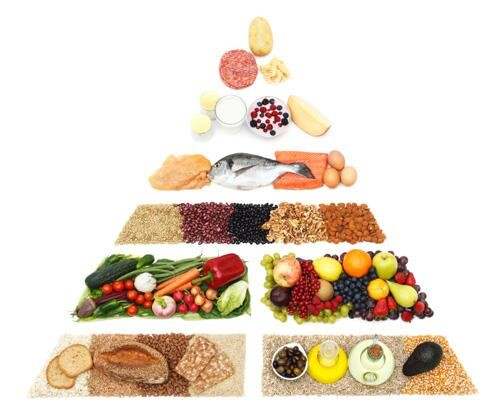
\includegraphics[width=0.6\textwidth]{img/mediterranean_diet_pyramid.jpg}
\end{center}


\textbf{Пирамида средиземноморской диеты.} Орехи – неотъемлемая часть средиземноморской диеты. Но поскольку они высококалорийные, желательно съедать в день не больше горсточки, которая помещается в одной ладони. Также средиземноморская диета содержит много бобовых. Постарайтесь постепенно вводить в свой рацион бобовые – фасоль, нут, горох, чечевицу. На их основе можно готовить супы и другие блюда.

Основной источник жиров в средиземноморской диете – это оливковое масло, которое содержит мононенасыщенные жиры. Если заменить насыщенные жиры (сливочное масло, мясо и т.п.) оливковым маслом, в организме снижается уровень «плохого» холестерина – липопротеидов низкой плотности. Лучше использовать оливковое масло, прошедшее наименьшую обработку, – «extra-virgin» и «virgin». Оно содержит максимум антиоксидантов.

Средиземноморскую диету невозможно представить без рыбы и морепродуктов. Жирная рыба (скумбрия, радужная форель, сардина, лосось, сельдь) богата на омега-3 жирные кислоты, полезные для здоровья кожи и сердечно-сосудистой системы. Средиземноморская диета предполагает умеренное употребление яиц и молочных продуктов – сыров и йогурта. Желательно выбирать продукты с низким содержанием жиров. Красное мясо появляется на столе всего лишь 1-2 раза в месяц. Это не повседневная еда, а, скорее, деликатес, которым можно себя изредка побаловать.


Некоторые научные исследования указывают на то, что умеренное употребление вина снижает риск заболеваний сердца. Но при этом важно понимать, что такое «умеренное употребление». Для женщин – это 150 мл (1 бокал) вина, а для мужчин – 300 мл (2 бокала) в день. При этом дневные дозы нельзя «накапливать». Если вы не пили всю неделю, это не означает, что на выходных можно опустошить всю бутылку.

Попробуйте средиземноморскую диету. Она не предполагает резкого ограничения килокалорий и не вызывает чувство голода. Замените красное мясо рыбой и птицей, сливочное масло – оливковым маслом, сладости – фруктами и орехами. Это простой и безопасный путь к здоровью.

\textbf{Комментарий врача Универсальной клиники «Оберіг»:} Средиземноморская диета является универсальной для профилактики и лечения большинства возрастных болезней цивилизационного мира.

Кроме общеизвестной пользы Омега-3 жирных кислот, которые содержатся преимущественно в морской рыбе, один из важнейших принципов заключается в ежедневном употреблении полезных растительных жиров, которые содержатся в оливковом масле и расширение ежедневного рациона за счет овощей, салатов.

Скажете, что данные принципы можно соблюдать только в странах Средиземноморья и только в летний период? На самом деле, в украинских традициях тоже возможна вкусная и полезная модификация. Так, Омега-3-ненасыщенные жирные кислоты содержатся также в семенах тыквы, льна, грецких орехах и арахисе, бобовых, яйцах, шпинате, капусте и мяте. В зимнее время года полезным будет употребление украинских аналогов средиземноморской диеты – свекольно-морковных салатов, овощных супов, винегрета (исключая картофель), при этом оливковое масло первого отжима можно заменить на нерафинированное подсолнечное, льняное, рапсовое, горчичное или соевое.


Соблюдение данных принципов способствует регулярной эвакуации желчи, нормализует работу желудочно-кишечного тракта, налаживает метаболизм, уменьшает уровень холестерина и риски сердечно-сосудистых осложнений.




\section{Курение вредит вашему здоровью}
Источник: \url{https://novo-sibirsk.ru/news/266296/}

Основным веществом для табачных изделий является никотин. В равных количествах он более ядовит, чем стрихнин, и обладает в 3 раза большей токсичностью, чем мышьяк. Табачный дым в 4,5 раза токсичнее автомобильных выхлопов и в 248 раз - дыма газовой горелки.

К настоящему времени в табачных изделиях обнаружено около 4000 химических соединений, а в табачном дыме около 5000, из них около 60 веществ являются известными или предполагаемыми канцерогенами.

Смертельная доза для взрослого человека 60 мг никотина, а для детей еще меньше.

В невыкуренной сигарете содержится порядка 10 мг никотина, но через дым курильщик получает от одной сигареты порядка 3 мг никотина.

Главная опасность никотина заключается в том, что никотиновая зависимость поддерживает потребление табака. Никотиновая зависимость формируется очень быстро. Как правило, многие молодые курильщики недооценивают риск развития зависимости. Однако 98\% регулярных курильщиков, пробующих отказаться от курения, терпят неудачу сразу или начинают курить снова в течение года.

Температура табачного дыма, поступающего в рот при курении, на 35-40 градусов выше температуры воздуха и вызывает во рту довольно резкий перепад температур. Во время курения одной сигареты происходит 15-20 таких перепадов, что плохо отражается на состоянии зубной эмали: она трескается. Вот почему зубы курильщика разрушаются раньше, чем зубы некурящих.

При выкуривании 1 пачки сигарет курильщик производит около 1 грамма жидкого дегтя, который оседает на пальцах, в бронхах, легких, попадает в желудок.

Курение приводит к развитию трех основных заболеваний с летальным исходом: рак легкого; хронический бронхит и эмфизема; коронарная болезнь. 90\% онкологических заболеваний вызвано курением табака. Подсчитано, что у людей, начавших курить с 15-летнего возраста, он возникает в 5 раз чаще, чем у тех, кто закурил позже 25 лет. Продолжительность жизни курящего человека сокращается на 20-25 лет.

При выкуривании 20 сигарет в день за год курильщик получает дозу облучения, соответствующую дозе от 200 рентгеновских снимков.

У молодых курящих женщин поражаются вены нижних конечностей с последующим развитием у них эктазий, варикоза, тромбозов. Наблюдается повышенный риск возникновения ишeмической болезни сердца, инфаркта миокарда, мозгового инсульта, частота развития которого в 20 раз выше, чем у некурящих.


\section{Вред алкоголя, его влияние на организм человека }

Источник: \url{http://pol1.tomsk.ru/novosti/281-21-09-2018}

Алкоголь – штука коварная: с одной стороны, бокал пива – просто незаменимое лекарство от перенапряжения после тяжелой рабочей недели. Но с другой – это невидимый, но достаточно ощутимый удар по здоровью, бьющий в самые уязвимые места нашего организма.

О семи причинах, почему стоит отказаться от алкогольных напитков и о том, как они способны навредить твоей жизни – далее в нашей статье.

1. Удар по сердечно-сосудистой системе. Как только алкоголь попадает в организм, сердце начинает увеличиваться в размере (особую коварность таит в себе пиво). На тканях сердца появляются многочисленные рубцы, которые являются виновниками инфаркта и способны привести к смерти.

2. Затуманенный рассудок. Алкоголь не зря считается разновидностью наркотических веществ: спиртные напитки оказывают на психику эйфорическое воздействие, продолжительность которого составляет от часа до полутора. Вскоре после этого человек впадает в депрессивное состояние, сопровождающееся агрессией и приступами панического страха. Реакции снижаются, о ясном мышлении в такой ситуации не может быть и речи. Именно по этой причине, как известно, водителям нельзя пить: вождение в нетрезвом виде может закончиться самым плачевным исходом.

3. Уничтожение клеток мозга. Даже небольшое количество алкоголя (да, полбокала вина также сюда относится) уничтожает несколько тысяч нейронов без возможности восстановления. Спирт, содержащийся в алкогольных напитках, провоцирует склеивание эритроцитов – красных кровяных телец: последние закупоривают микрокапилляры, приводя к смерти нейронов от кислородного голодания. Клетки, павшие в неравном бою с алкоголем, выводятся из организма с мочой.

4. Развитие хронических болезней. Медики приравнивают действие алкоголя к медленному яду: продукты распада спирта разрушают организм в прямом смысле слова. Человек, регулярно употребляющий спиртное, со временем все чаще начинает ощущать недомогание, его умственная и физическая активность заметно снижаются, на смену им приходит апатия. Длительная алкогольная зависимость – залог развития таких опасных хронических болезней, как панкреатит, рак поджелудочной железы, цирроз, инфаркт и масса других коварных заболеваний. Не самая обнадеживающая перспектива, не так ли?

5. Плохая наследственность. Алкоголь вносит изменения в структуру генетического кода ДНК – именно она содержит в себе информацию о человеке и его потомках. Ученые давно пришли к выводу, что 90\% детей с отклонениями в умственном развитии и врожденных инвалидов рождаются у людей, злоупотребляющих спиртными напитками.

6. Непристойное поведение. Уверены, тебе не раз приходилось наблюдать, что из себя представляет пьяный человек: алкоголь оказывает влияние на нравственные центры головного мозга, в связи с чем его дальнейшее поведение становится абсолютно непредсказуемым. В лучшем случае, все заканчивается мирным посапыванием в укромном уголке. В худшем – неконтролируемой агрессией, вспышками гнева и другими малоприятными вещами, которые в трезвом виде человек ни за что бы себе не позволил.

7. Дыра в бюджете. Цены на алкоголь (особенно хороший) немалые, и регулярное распитие любимых спиртных напитков зачастую влетает в немалую копеечку. К тому же, люди, которые начали испытывать зависимость от алкоголя, на одной бутылке не останавливаются: чем сильнее “захмелевает” голова, тем больше напитка будет куплено. Даже банальный просмотр футбольного матча практически никогда не обходится без нескольких банок пива – что уж говорить о пикнике с компанией, рыбалке или дне рождения. Если подсчитать, в какую сумму обходится такой досуг, действительно возникнет желание отложить эти деньги для более разумных целей (вложить в путешествие или же, к примеру, порадовать себя новым гаджетом).

Как видишь, существует масса причин как можно реже притрагиваться к спиртному, а то и вовсе от него отказаться. Да, алкоголь создает эффект расслабления. Да, он раскрепощает и снимает внутренние зажимы. Но тот вред, который организм получает параллельно, сводит “на нет” и без того небольшие преимущества. К тому же, расслабиться можно и другими способами – йога, плавание, горячая ванна, сауна, массаж или же неспешная прогулка в спокойном зеленом парке являются лучшими помощниками в этом деле. Позаботься о собственном здоровье сейчас, и в будущем у тебя будет в разы больше шансов избежать больничной койки и массы других малоприятных “бонусов”, нажитых за годы употребления алкоголя.

\section{Восемь советов как избежать стресса}
Источник: \url{https://primamedia.ru/cards/health04/}

Суетливая повседневность, напряженность, проблемы, которые ежедневно нас беспокоят, нарушают наше психическое равновесие и спокойствие. Эксперты убеждены, что для эффективного управления стрессом мы должны быть достаточно мотивированы и сами выстраивать стратегию, которая поможет нам в трудные времена.

Эти советы могут быть полезны при нашем повседневном стрессе - они усилят энергию и поддержат жизненный тонус.

\textbf{1. Лестница вместо лифта.}
Когда мы пребываем в унынии, то частенько «успокаиваем» себя конфетами, сигаретой или чашечкой кофе. Гораздо лучшим вариантом является физическая активность.

В состоянии стресса или гнева попробуйте больше двигаться. Можно подняться по лестнице или совершить быструю прогулку. Даже 10 минут упражнений улучшат настроение и повысят энергетику.

\textbf{2. Еда снижает стресс. Миф! Насытьте себя «воздушной смесью».}
Вы пытаетесь снять стресс пищей? Многие считают, что это приносит комфорт, по крайней мере, в краткосрочной перспективе. Самообман.

В напряженные моменты ешьте фрукты или овощи. Это хоть предотвратит накопление лишних килограммов.

Попробуйте вместо еды, в стрессовой ситуации, сделать несколько глубоких вдохов.

\textbf{3. Полноценный сон делает нас более гармоничными.}
Качество сна – это способ борьбы с нервными состояниями. Нужно 7-9 часов сна, чтобы уменьшить стресс и подзарядиться для следующего дня.

Если у вас проблемы с засыпанием, ограничьте потребление кофеина. Избегайте тренировки за два часа до сна. Удалите из своей спальни телевизор, домашних животных, компьютер и другие «отвлекашки».

\textbf{4. Выбирайтесь из рутины.}
Даже небольшие изменения в повседневной жизни помогут улучшить настроение.

Найдите другие маршруты для похода на работу или прогулки с собакой. Измените меню завтрака или ужина.

Сосредоточьтесь на легко достижимых изменениях, чтобы добиться гарантированного успеха.

\textbf{5. Прогулка по окрестностям.}
Вам не нужно часами пыхтеть в тренажерном зале. Даже небольшие телодвижения могут быть полезны для восстановления вашей энергетики.

Простая прогулка по ближайшему скверику поможет освежить ум. Упражнения на свежем воздухе, включающие медитацию, йогу или ци-гун, помогают зарядить не только ум, но и тело.

\textbf{6. Больше волокнистой пищи!}
Получение достаточного количества клетчатки полезно для улучшения пищеварения и поддержания здоровья сердца.

Много волокон находится в овсяной муке, цельнозерновом хлебе и крупах, овощах и фруктах (в яблоках, клубнике, цитрусовых).

\textbf{7. Сосредоточьтесь на сегодняшнем дне.}  Оставьте свои мысли о прошлом или будущем, сосредоточьтесь на текущем моменте. Важно знать, где вы находитесь именно сейчас! Направьте свою энергию на то, что вы делаете в данный момент! Насладитесь тем, что с вами происходит!

\textbf{8. Не пренебрегайте здоровьем.} Мы стараемся игнорировать головную боль, «раздражающий» кашель, усталость или другие лёгкие недомогания. Но это всё влияет на наше психическое состояние, включая нашу жизнеспособность. Поэтому в случае симптомов и подозрений по поводу здоровья, рекомендуется своевременно обратиться к врачу.

Полезно внимательно слушать и уважать себя и свой организм!


\section{Диабет}
Источник: \url{https://www.who.int/ru/news-room/fact-sheets/detail/diabetes}

\textbf{Основные факты.}
\begin{enumerate}
    \item За период с 1980 по 2014 г. количество людей, страдающих диабетом, выросло со 108 миллионов до 422 миллионов. В странах с низким и средним уровнем дохода распространенность диабета растет быстрее, чем в странах с высоким уровнем дохода.
    \item Диабет является одной из ведущих причин слепоты, почечной недостаточности, сердечных приступов, инсульта и ампутации нижних конечностей.
    \item С 2000 по 2016 г. преждевременная смертность от диабета увеличилась на 5\%.
    \item В 2019 г. диабет стал девятой ведущей причиной смерти в мире и, согласно оценкам, непосредственной причиной 1,5 миллиона случаев смерти.
    \item Здоровое питание, регулярная физическая активность, поддержание здоровой массы тела и воздержание от употребления табака могут предупредить или отсрочить возникновение диабета 2-го типа.
    \item Диабет поддается лечению, а диета, физическая активность, медикаментозное лечение и регулярный контроль и лечение осложнений помогают предупредить или задержать наступление его последствий.
\end{enumerate}

Диабет — хроническая болезнь, развивающаяся в тех случаях, когда поджелудочная железа не вырабатывает достаточно инсулина или когда организм не может эффективно использовать вырабатываемый им инсулин. Инсулин — это гормон, регулирующий уровень содержания сахара в крови. Распространенным следствием неконтролируемого диабета является гипергликемия, или повышенный уровень содержания сахара в крови, со временем приводящая к серьезному повреждению многих систем организма, особенно нервов и кровеносных сосудов.

В 2014 г. заболеваемость диабетом среди взрослого населения в возрасте 18 лет и старше составляла 8,5\%. В 2019 г. диабет стал непосредственной причиной 1,5 миллиона случаев смерти, и 48\% всех связанных с диабетом случаев смерти произошли в возрасте до 70 лет.

С 2000 по 2016 г. преждевременная (т. е. в возрасте до 70 лет) смертность от диабета увеличилась на 5\%. В странах с высоким уровнем дохода показатель преждевременной смертности от диабета снижался с 2000 по 2010 г., но затем вновь увеличился в 2010–2016 гг. В странах с уровнем дохода ниже среднего прирост преждевременной смертности от диабета имел место в оба этих периода.

По сравнению с этим, за период с 2000 по 2016 г. вероятность наступления смерти в возрасте от 30 до 70 лет по причине неинфекционных заболеваний, принадлежащих к одной из четырех основных групп (сердечно‑сосудистые, онкологические, хронические заболевания органов дыхания или диабет), снизилась во всем мире на 18\%.

\textbf{Диабет 2‑го типа.} Диабет 2‑го типа (ранее — инсулиннезависимый или диабет взрослых) развивается в результате неэффективного использования инсулина организмом. Диабетом 2‑го типа страдает более 95\% диабетиков. Данный тип диабета возникает, главным образом, на фоне избыточной массы тела и недостаточной физической активности.

Его симптомы могут быть сходными с симптомами диабета 1‑го типа, но часто менее выражены. В результате болезнь нередко диагностируется по прошествии нескольких лет после ее возникновения, уже после появления осложнений.

До недавнего времени диабет этого типа наблюдался лишь среди взрослых, однако в настоящее время он все чаще поражает и детей.

\textbf{Диабет 1‑го типа.} При диабете 1‑го типа (ранее – инсулинозависимый, юношеский или детский), для которого характерна недостаточная выработка инсулина, пациенту требуется ежедневное введение инсулина. В 2017 г. в мире было зарегистрировано 9 миллионов больных диабетом 1‑го типа, причем большинство из них проживали в странах с высоким уровнем дохода. В настоящее время причина этого типа диабета неизвестна, а меры профилактики не разработаны.

Симптомы включают чрезмерное мочеотделение (полиурия), жажду (полидипсия), постоянное чувство голода, потерю веса, нарушения зрения и усталость. Эти симптомы могут появиться внезапно.

\textbf{Гестационный диабет.} Гестационный диабет проявляется гипергликемией с показателями глюкозы крови, которые превышают нормальные, однако не достигают диагностически значимых для постановки диагноза диабета. Гестационный диабет имеет место во время беременности.

Женщинам с такой формой диабета угрожает повышенный риск осложнений во время беременности и родов. Они и, возможно, их дети подвергаются повышенному риску дальнейшего развития диабета 2‑го типа.

Чаще всего гестационный диабет диагностируется не по жалобам пациентки, а при проведении пренатального скрининга.
Снижение толерантности к глюкозе и нарушение гликемии натощак

Пониженная толерантность к глюкозе (ПТГ) и нарушение гликемии натощак (НГН) являются промежуточными состояниями между нормой и диабетом. Люди с ПТГ и НГН подвергаются высокому риску развития диабета 2‑го типа, однако этого может и не произойти.


\textbf{Последствия диабета для здоровья.}
Со временем диабет может приводить к поражению сердца, кровеносных сосудов, глаз, почек и нервов.

У взрослых людей с диабетом в 2–3 раза выше риск развития инфаркта и инсульта (1).

В сочетании со снижением кровотока невропатия (повреждение нервов) нижних конечностей повышает вероятность появления на стопах язв, инфицирования и, в конечном счете, необходимости ампутации.

Диабетическая ретинопатия, являющаяся одной из важных причин слепоты, развивается в результате долговременного накопления повреждений мелких кровеносных сосудов сетчатки. С диабетом связан почти один миллион случаев слепоты во всем мире (2).

Диабет относится к числу основных причин почечной недостаточности (3).

\textbf{Профилактика.} Известно, что простые меры по поддержанию здорового образа жизни способствуют профилактике диабета 2‑го типа либо позволяют отсрочить его возникновение. Для повышения шансов на предупреждение диабета 2‑го типа и связанных с ним осложнений, необходимо:

добиться здоровой массы тела и поддерживать ее; поддерживать физическую активность — по меньшей мере 30 минут регулярной активности умеренной интенсивности в течение большинства дней; для контроля веса необходима дополнительная активность; придерживаться здорового питания и уменьшать потребление сахара и насыщенных жиров; и не употреблять табак — курение повышает риск развития сердечно-сосудистых заболеваний.


\section{Пять причин делать утреннюю зарядку}
Источник: \url{https://med-atlant.ru/news/5-prichin-delat-utrennyuyu-zaryadku/}

Утреннее пробуждение всегда сопряжено с сонливостью и даже некоторой ленью. Чтобы взбодриться, некоторые люди тут же заваривают себе ароматный кофе, другие начинают день с принятия душа. И только немногие пробуждаются при помощи утренней зарядки. Как показывает практика, именно те, кто взбадривает организм физкультурой, быстрее переходят в активный режим. Итак, в чем же польза зарядки? Для чего она нужна? И какие упражнения лучше делать по утрам?

Приходилось ли вам замечать, как много людей утром в плохом настроении? Врачи считают, что одна из причин такого состояния заключена в гипокинезии. Иными словами, в отсутствии физической активности. Ничего удивительного. Проработанные мышцы посылают в головной мозг достаточное количество импульсов, благодаря которым он активно настраивается на рабочий лад.

Люди, которые отказываются от утренней зарядки, часто страдают от нервной возбудимости, испытывают хроническую усталость. Они жалуются на отсутствие энергичности и бодрости утром. И только к полудню такие люди отмечают повышение активности.

\textbf{Зачем нужна зарядка.}
Организм человека не способен полностью пробудиться по звонку будильника. И даже в тот момент, когда вы уже поднялись с кровати, все внутренние органы и системы еще продолжают «отдыхать».

Во время сна замедляется циркуляция крови, затормаживается метаболизм, снижается умственная деятельность. Именно поэтому во время пробуждения человек ощущает легкую заторможенность. У него отмечается сниженная работоспособность, как физическая, так и умственная. Утром значительно ухудшена скорость реакций.

Такое состояние может длиться (в зависимости от индивидуальных особенностей) от 1 до 3 часов. Чтобы полностью проснуться и стряхнуть подобную «заторможенность», необходимо разработать суставы и мышцы. Другими словами, нужно просто сделать зарядку.

\textbf{Какая польза от зарядки?}
С самого детства родители твердили нам о необходимости делать зарядку. Лишь немногие безропотно прислушались к таким рекомендациям. А большая часть людей, прежде чем начать делать утреннюю зарядку, стремится понять, что же такого ценного она приносит.

Физическая активность в утреннее время обеспечивает следующее.

\textbf{Придает бодрость.} Организм человека просыпается значительно быстрее и активнее, если была совершена даже небольшая зарядка. После физкультуры активизируется кровообращение. Все органы и ткани начинают активно насыщаться кислородом. Ощущается прилив энергии, улучшается самочувствие. Мозг, получивший свою порцию кислорода, активно включается в рабочий процесс.


\textbf{Улучшает физическую форму.} Регулярные занятия приводят к укреплению мышечных тканей. Физкультура положительно влияет на состояние позвоночника и суставов. Даже простая и недлительная гимнастика служит отличной профилактикой развития многих болезней опорно-двигательного аппарата.

Утренняя зарядка стимулирует метаболизм. Благодаря этому человек постепенно обретает красивые формы. Некоторые мышцы подкачиваются, появляется стройность, подтягивается живот.

\textbf{Повышает настроение.} Зачем делать зарядку, если можно взбодриться от чашки кофе? Увы. Это не так. Ароматный напиток не обеспечит той энергичности и позитива, которые подарит утренняя гимнастика.

Зарядка подразумевает набор простых упражнений, которые направлены на разогрев мышц и проработку суставов. Никаких чрезмерных нагрузок утренняя физкультура не содержит. А поэтому она не вызывает ощущения усталости или боли.

\textbf{Укрепляет силу воли.}   Приняв решение делать зарядку, вам необходимо заставить себя подниматься на 10-15 минут раньше. На первых порах при правильном настрое и соответствующей мотивации вы с легкостью преодолеете этот барьер.

Но со временем, приблизительно к 20-21 дню, могут начаться серьезные трудности. Положительные результаты к этому времени еще мало заметны. Поэтому начинают появляться навязчивые мысли: «Зачем мне нужна эта зарядка, она все равно ничего не дает. Лучше поспать лишние 10-15 минут». Вот именно в этот момент важно не поддаться таким мыслям и преодолеть себя. Такое «упражнение» здорово прокачает вашу силу воли.

\textbf{Укрепляет здоровье.}
Утренняя зарядка оказывает комплексное воздействие на организм. Она активизирует кровообращение, ускоряет обмен веществ. Благодаря улучшенному кровотоку все внутренние органы получают достаточное питание и начинают значительно активнее функционировать.

Польза утренней зарядки заключена в следующих воздействиях:

\begin{itemize}
    \item укрепление сердечной мышцы;
    \item улучшение работы дыхательной системы;
    \item повышение упругости мышц;
    \item нормализация состояния сосудов, повышение их проходимости;
    \item выравнивание осанки;
    \item усиление концентрации внимания;
    \item повышение подвижности суставов;
    \item стимуляция работы мозга;
    \item повышение выносливости;
    \item нормализация работы вестибулярного аппарата.
\end{itemize}

\textbf{Утренняя зарядка: основные правила и рекомендуемые упражнения.} Существует еще одно распространенное заблуждение. Некоторые люди уверенны, что не обязательно делать зарядку утром. Можно практиковать физическую активность после обеда и даже вечером. Если речь идет об утренней зарядке, то все специалисты сходятся в одном: она должна быть утром, после пробуждения. Ведь основная цель такой гимнастики – зарядить человека бодростью и энергией на весь день.

\section{Пять важных рекомендаций}
Источник: \url{https://med-atlant.ru/news/5-prichin-delat-utrennyuyu-zaryadku/}

Чтобы польза зарядки, выполняемой  по утрам, была максимальной, необходимо соблюдать следующие правила.

\textbf{Продолжительность гимнастикию.} Тем, кто только начинает вводить в свою жизнь утреннюю зарядку, рекомендуется планировать 10-минутную физкультуру. Со временем можно увеличить время до 15 минут. Когда организм полностью адаптируется к нагрузкам (приблизительно через 3-6 месяцев) начинайте увеличивать время зарядки до получаса.

\textbf{Подготовка к зарядке.} Не стоит приступать к гимнастике сразу после подъема с кровати. Организм еще продолжает спать. Такие нагрузки вызовут дискомфорт. Изначально нужно немного взбодриться. Для этого рекомендуется умыться, почистить зубы.

Обязательно выпейте стакан воды. Жидкость, поступившая в организм, обеспечит разжижение крови. Благодаря этому удастся нормализовать нагрузку на сердце и сосуды. А вот перекусывать перед зарядкой не стоит. Все упражнения выполняйте натощак.

\textbf{Добавьте эмоции.} Зарядка должна не только взбадривать, но и повышать настроение. Поэтому включайте любимую музыку, насыщайте воздух ароматными маслами (только не переусердствуйте) и занимайтесь гимнастикой. После физкультуры обязательно хвалите себя, отмечайте все достижения и не забывайте о поощрении.

Чтобы зарядка принесла значительную пользу для организма, предварительно проветрите помещение. Это можно сделать в то время, пока вы умываетесь. Приток свежего воздуха позволит насытить организм большим количеством кислорода.

\textbf{Регулярность занятий.} Если вы делаете зарядку от случая к случаю, то надеяться на положительные результаты не стоит. Пользу принесут только ежедневные занятия. Причем первые результаты станут заметны через 5-6 недель регулярных тренировок.

В это время люди обычно отмечают снижение уровня стресса, позитивный настрой, уменьшение возбудимости и раздражительности. Практикующие утреннюю зарядку утверждают, что к 5-6-й неделе усиливается работоспособность, повышается дисциплинированность и упорство. Люди становятся крепче и практически не подхватывают простуды.

\textbf{Правильный комплекс.} Еще один важный момент, который не следует упускать из виду, – это правильный комплекс упражнений. Гимнастика должна «запустить» все органы и ткани. Именно поэтому комплекс составляйте из упражнений, прорабатывающих все мышцы и суставы.



Утренняя зарядка должна включать в себя три этапа:
\begin{enumerate}
    \item Разминку. Ее можно делать лежа в постели. Она включает потягивание, дыхательные упражнения. В этот комплекс могут входить легкие вращательные движения кистями, стопами, конечностями.
    \item Основной комплекс. Он состоит из упражнений, прорабатывающих все мышцы и суставы. Начинают обычно с шеи, затем переходят на плечи, верхние конечности. Теперь очередь подходит к мышцам спины, живота. Заканчивают основной комплекс махами ногами.
    \item Завершение, или заминку. После основного комплекса рекомендована ходьба на месте и дыхательные упражнения.
\end{enumerate}



\section{Рекомендуемые упражнения}
Источник: \url{https://med-atlant.ru/news/5-prichin-delat-utrennyuyu-zaryadku/}

Особое внимание следует обратить на интенсивность нагрузок. Утренняя зарядка должна приносить пользу и заряжать энергией, а не истощать организм. Именно поэтому от тяжелых упражнений (с гантелями, штангой, на выносливость и т. д.) нужно отказаться. Интенсивные тренировки лучше всего проводить после обеда. А утром отдайте предпочтение легким, простым движениям.

Утренняя зарядка обычно включает следующие группы упражнений:
\begin{enumerate}
    \item \textit{Дыхательная гимнастика}. Она улучшает работу дыхательной системы и обеспечивает активный приток кислорода к внутренним органам.
    \item \textit{Ходьба}. Очень полезно ходить босыми ногами по полу. В этом случае массируются многие активные точки. Специалисты по нетрадиционной медицине утверждают, что именно на стопе их больше всего.
    \item \textit{Гимнастика для шеи}. Она включает повороты и наклоны головы. Такие упражнения должны выполняться очень осторожно, без надрывов. Полезны вращательные движения головой. Они не только укрепляют мышцы шеи, но и тренируют вестибулярный аппарат.
    \item \textit{Физкультура для верхних конечностей}. Обязательно выполняйте упражнения на поднятие рук вверх, разведение в стороны. Вращайте конечностями. Это способствует вытягиванию позвоночника и укреплению плечевого пояса.
    \item \textit{Упражнения для кистей и пальцев}. Такие занятия полезны тем людям, работа которых связана с руками (операторы ПК, музыканты, художники, ювелиры). Эта гимнастики активизирует кровообращение и укрепляет суставы.
    \item \textit{Физкультура для поясничного отдела}. В утреннюю зарядку нужно включать наклоны в разные стороны, вперед/назад. Если нет особых проблем с позвоночником, рекомендованы упражнения на скручивания. Полезны вращательные движения талией.
    \item \textit{Приседания}. Они повышают подвижность коленных и тазовых суставов. Кроме того, такие простые упражнения позволяют улучшить внешний вид икр и бедер.
    \item \textit{Упражнения на пресс}. Если вам совершенно не дает покоя животик или очень хочется сформировать рельефные кубики на животе, то включите в зарядку упражнения на пресс.
    \item \textit{Махи ногами и руками}. Такая гимнастика повышает тонус мышечных тканей и ускоряет кровообращение.
    \item \textit{Бег, прыжки}. Эти движения отлично прорабатывают все мышцы нижних конечностей. Кроме того, они значительно усиливают метаболизм.
\end{enumerate}
Если строгие комплексы навевают на вас тоску, то можете придумать свои собственные упражнения. Главное, чтобы они не истощали вас и прорабатывали все мышцы. Кстати, никто не запрещает вам просто танцевать под любимую музыку, периодически поднимая руки, совершая махи ногами и работая талией.


\section{Зачем нам нужны фрукты и овощи? Основы здорового питания!}
\textit{Автор: Юлия Баяндина.
    Источник: \url{https://www.shkolazhizni.ru/health/articles/63634/}}

С самого детства мы только и слышим — нужно есть свежие фрукты и овощи, в них много витаминов, они очень полезные. А почему? Этого никто не объясняет. Давайте разберемся, что нам это дает, и в чем состоит польза фруктов и овощей.

1. Поднимают настроение
Фрукты и овощи сродни шоколаду — содержат вещества (селен и фолиевую кислоту), которые способствуют выработке эндорфинов. Если что-нибудь не задалось — съешьте яблоко или банан, и настроение улучшится.

2. Дарят бодрость Фрукты и овощи содержат много воды — одновременно спасают и от голода, и от жажды, быстро усваиваются. Если нужен заряд бодрости — лучшего решения не найти. Поэтому утренний завтрак так полезно начинать с фруктов — и настроение поднимут, и энергией зарядят.

3. Добавляют витаминов Сколько фармацевты ни бьются над созданием супервитаминок, а идеального баланса найти не могут. Невозможно в одной таблетке уместить витамины так, чтобы все они полностью усваивались! С овощами и фруктами такой проблемы не возникает — все гармонично, все усваивается.

4. Помогают похудеть Овощи и фрукты содержат море клетчатки, которая почти не содержит калорий, но дает ощущение сытости. Поэтому их можно есть в любом количестве и не бояться лишнего веса — ему при таком рационе неоткуда будет взяться. Вдобавок клетчатка, словно липкая лента, собирает вредные химические вещества и канцерогены и выводит их из организма.

5. Спасают от холестерина Ничто так не страшно для сердечно-сосудистой системы, как избыток холестерина. Снизить его уровень в крови тоже помогут фрукты и овощи. Холестерин попадает в организм с животной пищей и вырабатывается печенью. В растительной пище холестерина нет, зато в ней есть пектин, который помогает выводить вредный холестерин из организма.

6. Продлевают молодость Помните молодильные яблочки из сказок? Так вот — они существуют. Сырые овощи и фрукты содержат антиоксиданты, которые помогают обновляться клеткам организма и предотвращают окисление органических соединений — попросту говоря, позволяют вам быть моложе и свежее.

7. Делают умнее Овощи и фрукты помогут сохранить ясность ума и отличную память: недавно опубликовали результаты исследования, в котором выяснили, что 6-8 фруктов и овощей в день помогают лучше запоминать и решать математические задачки. А еще фрукты и овощи спасают от заболеваний мозга: в знаменитой книге «Китайское исследование» пишут, что три порции фруктов и овощей каждый день помогут снизить риск инсульта. Одна порция -- это, к примеру, $\nicefrac{1}{2}$ чашки персиков, $\nicefrac{1}{4}$ чашки томатного соуса, $\nicefrac{1}{2}$ чашки брокколи или одна картофелина. Полчашки -- это немного.

8. Защищают от болезней Ученый Колин Кэмбелл 20 лет искал взаимосвязь между болезнями и питанием. Проверил рацион миллионов людей и доказал — фрукты и овощи лечат лучше любого доктора. Аргумент. И чем больше их в вашем рационе — тем ниже риск заболеть раком, диабетом и прочими страшными болезнями. Факт.

9. Экономят время Потому что их практически не надо готовить. Конечно, есть картофель сырым не стоит, но большинство фруктов перед едой достаточно просто вымыть. И в конце концов, фрукты и овощи — это просто очень вкусно!

% % Автор: Юлия Баяндина
% % Источник: https://www.shkolazhizni.ru/health/articles/63634/
% % © Shkolazhizni.ru


\section{Лекарство от всех болезней, кроме смерти}
\textit{Источник: \url{https://lenta.ru/articles/2022/09/24/tmin/}}

\textit{Что говорят врачи о пользе и вреде масла черного тмина}

Семена черного тмина использовали еще в Древнем Египте три тысячи лет назад. Во время раскопок одной из гробниц археологи обнаружили бутылочку с маслом, и последующая экспертиза установила, что его изготовили из тмина. Египтяне использовали масло как один из компонентов противоядия от укусов змей, как косметическое средство и глистогонный препарат, а также употребляли в пищу для улучшения пищеварения и работы почек и печени. Как используют черный тмин и масло из него в XXI веке, «Лента.ру» разбиралась с экспертами.

Масло черного тмина имело популярностью не только в Египте. О его свойствах писали в медицинских трактатах великие древние греки Диоскорид и Гиппократ.

В арабском мире популярности масла, помимо его целебных качеств, способствовали слова, приписываемые пророку Мухаммеду. В Коране упоминается, что он называл семена тмина «лекарством от всех болезней, кроме смерти».

\textbf{Как получают масло черного тмина}

Масло черного тмина добывают путем холодного отжима семян чернушки посевной. Это однолетнее травянистое растение семейства лютиковых имеет еще несколько названий: калинджи, сейдана (седана), черный тмин, римский кориандр.

Родиной черного тмина считаются Средиземноморье и Юго-Западная Азия, где, к слову, произрастает большинство самых популярных специй. Но сейчас калинджи растет и в Крыму, и в Средней Азии, и на Балканском полуострове, и в других местностях.

Трава эта неприхотлива: всходит в степи, лесу, в садах и посевах. Черный тмин считается сорной травой, но ради семян его культивируют.

\begin{center}
    \Large
    Масло черного тмина имеет светло-желтый или зеленовато-коричневый оттенок, обладает пряным запахом и вяжущим, терпким вкусом
\end{center}

Масло черного тмина насыщено витаминами и минералами. Богатый полезными микроэлементами состав сделал его востребованным в фармакологии, кулинарии и косметологии.


\textbf{Состав масла черного тмина}

Масло черного тмина состоит из жирных кислот: арахиновой, омега-9 и омега-6, миристиновой, пальмитолеиновой и других. Если регулярно принимать масло черного тмина, то организм пополнится следующими витаминами:


\begin{itemize}
    \item витамины группы В. Оказывают положительное действие на работу ЦНС, улучшают обмен веществ, снижают риск развития анемии;
    \item витамин А. Помогает сохранять зрение, повышает защитные функции организма, улучшает обмен веществ;
    \item витамин E. Важен для сохранения беременности;
    \item витамин D. Снижает риск возникновения сердечно-сосудистых заболеваний, рахита. Укрепляет кости;
    \item аскорбиновая кислота. Повышает иммунитет, снижает уровень «плохого» \item холестерина, повышает физическую выносливость.
\end{itemize}

«Также в составе тминного масла есть каротиноиды, биофлавоноиды, фосфатидил, фитостеролы, восемь незаменимых аминокислот и важный активный компонент — тимохинон, который является мощным антиоксидантом с противовоспалительным, иммуномодулирующим и тонизирующим действием», — пояснила «Ленте.ру» терапевт клиники превентивной и антиэйдж-медицины Verba Mayr Мария Веригина.

\begin{fancyquotes}
    {\Huge 896 ккал}\\

    содержится в 100 граммах масла черного тмина
\end{fancyquotes}


\textbf{Польза масла черного тмина}

«Масло черного тмина помогает при язвенной болезни желудка, гастрите, энтерите, заболеваниях желчного пузыря и желчевыводящих путей, регулирует кислотность в желудке, — рассказала «Ленте.ру» диетолог Кристина Плотникова. — Но не стоит забывать, что это не лекарство, а сопутствующая вспомогательная терапия, и все заболевания должен лечить врач».

Масло черного тмина содержит вещества, которые могут снизить отечность, смягчить аллергические реакции, усилить иммунитет и даже отчасти помочь организму в борьбе с раковыми клетками.

Масло черного тмина имеет следующие свойства:

\begin{itemize}
    \item обезболивающее;
    \item противовоспалительное;
    \item антисептическое;
    \item бактерицидное;
    \item антивирусное;
    \item противопаразитарное;
    \item ранозаживляющее;
    \item антигрибковое;
    \item иммуностимулирующее.
\end{itemize}

\textbf{Воздействие масла черного тмина на организм}

Существует ряд исследований, доказывающих пользу масла черного тмина при лечении ряда недугов. Но стоит помнить, что его эффект пока не до конца изучен, а любая пищевая добавка не может заменить полноценного лечения под руководством опытного врача. Медики напоминают: не существует волшебной таблетки, и, если не вести здоровый образ жизни, любое средство, каким бы полезным оно ни было, не поможет справиться с последствиями вредных привычек.

\textbf{Помогает бороться с раком}

Исследования на животных показали, что семена черного тмина могут остановить рост опухолевых клеток и снизить частоту возникновения опухолей. Однако влияние на человека до конца не изучено.

\textbf{Снижает воспаление и боль при артрите}

Ученые опытным путем доказали, что микроэлементы, которые входят в состав масла черного тмина, способны улучшать состояние пациентов с ревматоидным артритом. Во время исследования части группы из 43 женщин с этим диагнозом давали масло, а остальным — плацебо. Через месяц у пациентов, принимавших масло черного тмина, зафиксировали снижение уровня маркеров воспаления крови, а также снижение интенсивности боли и уровня отека суставов.

\textbf{Защищает сердце и сосуды}

Масло черного тмина оказывает благотворное воздействие на сердце и сосуды. Оно является хорошим средством профилактики гипертонии, варикоза, тромбоза, ишемической болезни, атеросклероза.

\textbf{Помогает при аллергии}

Во время исследований в США установили, что масло черного тмина уменьшает отек в носу, заложенность носа, соответственно, помогает справиться с насморком. Правда, по данным исследования, чтобы добиться явного эффекта, масло нужно принимать две недели.

Масло черного тмина благодаря противовоспалительным и антигистаминным свойствам также способно снизить проявление аллергии и помочь быстрее избавиться от аллергического ринита.

\textbf{Избавляет от папиллом}

Бородавки и папилломы появляются на теле из-за попадания в организм вирусов. Масло черного тмина может избавить от новообразований.

Для этого нужно ватный или марлевый тампон смочить в подогретом тминном масле. Затем тампон разместить на пораженном участке кожи. Оставить его нужно на 5-6 часов, поэтому тампон следует закрепить пластырем или бинтом. Для полного избавления от бородавок и папиллом процедуру надо повторять каждый день в течение месяца.

Однако стоит помнить, что масло избавляет лишь от внешних проявлений болезни. Использовать его следует одновременно с медицинскими препаратами, назначенными врачом.

\textbf{Помогает бороться с диабетом}

Черный тмин помогает снизить уровень сахара и холестерина в крови. Люди, принимавшие добавки черного тмина, имели более низкий риск осложнений при сахарном диабете II типа. Однако это воздействие растения на организм человека предстоит изучить дополнительно.

\textbf{Поддерживает здоровье ЖКТ}

Ученые пришли к выводу, что тминное масло способно наладить процесс пищеварения и работу органов желудочно-кишечного тракта. Употребление масла помогает не только устранить причину развития заболеваний, но и убрать симптомы: приступы тошноты и рвоты, изжогу и колики.

К тому же масло тмина способствует заживлению повреждений слизистой оболочки желудка и ускорению процесса выздоровления.

\begin{fancyquotes}
    {\Huge 3-6 недель}\\

    нужно использовать тминное масло для появления ожидаемого эффекта
\end{fancyquotes}

\textbf{Помогает справиться с панкреатитом}

Принимать тминное масло можно только после наступления ремиссии заболевания и после консультации с врачом. В период обострения панкреатита масло может навредить.

После введения масла черного тмина в рацион снижается интенсивность проявления таких неприятных симптомов, как дискомфорт после приема пищи, отсутствие аппетита, метеоризм. К тому же масло останавливает размножение патогенных микроорганизмов и грибков.

\textbf{Предотвращает развитие рака простаты}

Ученые выяснили, что антиоксидант тимохинон способен подавлять рост раковых клеток в предстательной железе. Онкологи сходятся в мнении, что альтернативная медицина становится важной в качестве дополнительной терапии для больных раком, как для смягчения побочных эффектов химиотерапии, так и для усиления их противоопухолевых эффектов.

\textbf{Помогает бороться с простудой}

При простуде можно использовать масло черного тмина несколькими способами.

\begin{enumerate}
    \item Прием внутрь. Облегчить течение простуды поможет чай с тминным маслом. Но этот напиток является лишь дополнением к назначенной врачом терапии.
    \item Растирание. Грудную клетку можно растирать смесью из масла черного тмина и любого другого масла в пропорции 1:5 соответственно. Растирание поможет ослабить интенсивность кашля.
    \item Распаривание ног. Масло тмина обладает согревающим эффектом. Его добавляют в емкость с горячей водой, затем греют в ней ноги. Для большей эффективности в воду можно добавить порошок горчицы.
\end{enumerate}

\textbf{Избавляет от запора}

Тминное масло — отличное средство лечения и профилактики запоров. Оно улучшает перистальтику кишечника, размягчает каловые массы, выводит их без применения лекарственных препаратов. Особенно полезно масло как средство от запоров при беременности, во время грудного вскармливания, при нормализации стула у детей — в случаях, когда нежелательно пить лекарства.

Избежать запоров поможет масло черного тмина с чаем. Для этого нужно половину чайной ложки масла добавить в стакан чая и пить этот напиток дважды в день.

\textbf{Помогает людям с ожирением}

Масло черного тмина может помочь женщинам, страдающим ожирением. Во время исследований часть участниц научного эксперимента принимала плацебо, другая — масло. В конце исследования у участниц, принимавших масло, снизился вес, уменьшился обхват талии и уровень триглицеридов.

Исследователи также обнаружили, что сочетание диеты с приемом масла черного тмина и физическими упражнениями приводит к потере веса и снижению уровня холестерина.

Комментируя этот факт, эндокринолог клиники «РЖД-Медицина» в Твери Анна Куликова пояснила, что, согласно принципам рационального питания, следует ограничить прием всех растительных масел до столовой ложки в сутки (17 граммов). «Растительное масло, в том числе и масло черного тмина, — это на 99 процентов жир. Поэтому не стоит забывать о калорийности, ведь 100 граммов тминного масла — это почти 900 килокалорий!» — предупредила она.


\begin{fancyquotes}
    Масло черного тмина может оказывать положительное действие на организм. Входящие в его состав полезные вещества могут косвенным образом оказывать помощь в похудении. Но волшебной таблетки для избавления от лишнего веса не существует. 95-99 процентов случаев избытка массы тела связаны с перееданием и малой физической активностью.\\

    \begin{flushright}
        Анна Куликова, эндокринолог
    \end{flushright}
\end{fancyquotes}

\textbf{Облегчает состояние при астме}

Множество исследований черного тмина показали, что он облегчает состояние пациентов с бронхиальной астмой. Он оказал бронхолитическое, антигистаминное, противовоспалительное, антилейкотриеновое и иммуномодулирующее действие. Кроме того, клинические исследования установили, что при употреблении черного тмина улучшились лабораторные показатели анализов пациентов и работа легких.

\textbf{Спасает от паразитов}
Тминное масло стимулирует выработку лизоцима, способного остановить размножение глистов и других паразитов. Содержащиеся в масле элементы оказывают губительное воздействие не только на взрослых паразитов, но и их личинки.

Масло черного тмина действует следующим образом.

\begin{itemize}
    \item Убивает гельминтов, глистов, других паразитов, а также их яйца и личинки.
    \item Выводит паразитов из организма человека.
    \item Выводит из организма человека продукты жизнедеятельности паразитов — токсины.
    \item Восстанавливает пораженные паразитами ткани.
\end{itemize}

\textbf{Избавляет от геморроя}

Тминное масло входит в состав мазей и ванночек для лечения геморроя. Оно помогает снять или уменьшить болевой синдром, остановить кровотечение, упростить процесс дефекации, снять воспаление, повысить эластичность кожи и защитить ее от микротрещин.

Для избавления от геморроя нужно выпивать 2,5 миллилитра (чайная ложка) масла черного тмина утром и вечером. Но перед этим стоит проконсультироваться с врачом.

Также масло можно нанести на пораженный участок с помощью ватного тампона. Семена тмина можно добавлять в еду, смешивать с водой и медом.

[...]

\chapter{Музыка, художники и тексты песен}

\section{Пётр Налич}
Пётр Андреевич Налич (род. 30 апреля 1981, Москва) --- российский певец и композитор. Пишет песни, музыку к спектаклям, фильмам и мультфильмам.

В первый раз имя Петр Налич \explain{прозвучало}{звучать/прозвучать: to sound (here: was heard)} в 2007 году, когда Петр снял клип на свою песню «Гитар» и выложил её в интернет. Клип вошёл в ТОП-20 самых просматриваемых российских клипов русской версии ютьюба.

С 2008 года в составе МКПН (Музыкальный коллектив Петр\'{а} Налича) пел и \explain{сочинял}{сочинять/сочинить: to compose} песни в стиле, который сам характеризует как «веселые бабури». \explain{Представил}{представлять/представить: (here) to introduce} Россию на конкурсе Евровидение 2010 как \explain{победитель}{winner} отб\'{о}ра, \explain{прошедшего}{прошедший: past participle of пройти} 7 марта 2010 года. Пётр Налич стал первым артистом в истории российской музыкальной индустрии, выпустившим в Интернете альбом («Радость простых мелодий») с использованием системы Pay What You Want («Заплати, сколько хочешь»)

\textbf{1981--2006: детство, юность.}
Пётр Налич родился в Москве в семье архитекторов Андрея Захидовича и Валентины Марковны. Старший брат Павел --- художник-оформитель. По \explain{происхождению}{происхождение: origin (here: by origin)} --- дед по отцовской линии --- лирический тенор и диктор югославской редакции Московского радио (с 1993 года --- «Голос России»), Захид Омерович Налич был бошняком из города Тузла в Боснии и Герцеговине.

{\it «Мой дед --- босниец. Был до войны лирическим тенором. Имел ангажемент в Белградской опере. Но потом война, лагерь, там ему фашисты гортань сломали, больше он не пел. Потом он попал в Советский Союз и здесь всю жизнь работал на радио»}.

Налич рассказывал, что его «папа \explain{частенько}{quite often} пел за столом... Это и цыганские песни, и романсы» . Пётр Налич окончил детскую музыкальную школу им. Мясковского, обучался в музыкальном училище при Московской консерватории им. П. И. Чайковского, а также в студии «Орфей» \explain{под руководством}{under the direction of} Ирины Мухиной. В 2010 году поступил в РАМ имени Гнесиных на специальность «Академическое пение» (класс проф. В. Левко). Среднее образование получил в школе No 1278. Пётр рассказывал, что в школе пел в хард-роковой группе: «Когда голос у меня сломался, стал громким, я стал петь с удовольствием. Вообще я всю жизнь пою. Я музыкальную школу закончил, играли в хард-рок в школе, потом в институте продолжил заниматься музыкой. Чуть позже начал заниматься вокалом и только тогда понял, что пою не очень хорошо».

\textbf{2006--2007: начало карьеры.}
Творчество Петр\'{а} Налича \explain{приобрел\'{о}}{приобретать/приобрести: to gain; to acquire}
известность после того, как он опубликовал на YouTube самостоятельно сделанный клип
на собственную песню «Гитар».
Клип был выложен весной 2007 года. А осенью, в течение одного месяца, клип посмотрело 70000 человек.
Ссылку на р\'{о}лик \explain{пересыл\'{а}ли}{пересылать/переслать: to forward}
друг другу пользователи Livejournal, число просмотров прирастало в день на тысячу. Затем в нескольких \explain{печатных}{печатный/печатные: printed} \explain{изданиях}{издание: publication} появились интервью с Петр\'{о}м и статьи о нём. \explain{Публика}{the public} \explain{потребовала}{требовать/потребовать: to demand} \explain{явления}{явление, the audience demanded the appearance of the artist} артиста.

У Петр\'{а} на тот момент было написано около 40 песен и музыкальных композиций, все они были выложены в свободном \explain{д\'{о}ступе}{д\'{о}ступ: access} на его сайте --- энтузиасты собрали из них архив, который до сих пор можно найти в интернете. Этот материал \explain{лёг}{ложиться/лечь: to lie down (past tense: лёг, легл\'{а}, легл\'{о}, легл\'{и})} в основу репертуара, с которым Пётр 9 ноября 2007 года дал свой первый концерт в клубе «Апшу».

Из-за ажиот\'{а}жа многие не смогли попасть \explain{внутрь}{same as внутри: inside} переполненного зрителями \explain{помещения}{помещение: premises}. Концерт прошёл успешно, появились статьи, \explain{\'{о}тзывы}{\'{о}тзыв: review} в блогах и прессе. Тогда Пётр собрал группу музыкантов и зимой 2008 года дал ещё два концерта в клубе «Икра». Билеты на эти концерты были раскуплены задолго до события. Группа получила название «Музыкальный коллектив Петр\'{а} Налича» (сокращённо МКПН).

    {\it  ``Гитар'' я сочинил года четыре тому назад, а клип записали этой весной. Снимали у меня на даче по Щелковскому шоссе. Мы просто тусовались, веселились. У нас там стояла убитая ``копейка'' друга моего брата, которую он никак не мог забрать. Все уже \explain{злились}{злиться: to get angry}, что она стоит на участке. Ну и решили её \explain{употребить}{употреблать/употребить: to use; to consume}, раз уж она здесь. \explain{Набились}{?} в неё все... ну, а дальше вы знаете.}

\textbf{2007---2010: первый альбом, участие в конкурсе «Евровидение».}
В течение двух следующих лет, помимо концертов в Москве, МКПН посетил с гастролями Петербург, Екатеринбург, Нижний Новгород и другие большие города России. Летом 2008 года МКПН поддерживал российские спортивные команды на Чемпионате Европы по футболу и Олимпиаде-2008 в Пекине. Затем коллектив выпустил свой первый альбом --- «Радость простых мелодий», фильм-концерт «МКПН в Б1 Maximum» и макси-сингл «Море». В 2009 году группа выступила хедлайнером на международном фестивале «Sfinks» в Антверпене.

7 марта 2010 года «Музыкальный коллектив Петр\'{а} Налича» с песней «Lost and Forgotten» был выбран в качестве участника от России на конкурс «Евровидение». Выступление на конкурсе в Осло принесло 11-е место.

\textbf{2010---2012: второй и третий альбомы}
6 апреля 2010 года прошёл первый концерт, на котором Пётр Налич исполнял не свои песни, а классический оперный репертуар и романсы. С тех пор подобные концерты проводятся регулярно. В 2010 году группа выпустила второй студийный альбом «Весёлые Бабури». Продажи стартовали 9 октября в клубе «Арена», а с 11 октября --- в музыкальных магазинах города.

С 2011 года Пётр Налич принимает участие в спектаклях театра-студии оперы РАМ имени Гнесиных под руководством проф. Ю. А. Сперанского. Спел партии Рудольфа в опере «Богема» Дж. Пуччини и Ленского в спектакле по опере П. И. Чайковского «Евгений Онегин».

Осенью 2012 года вышел третий альбом коллектива --- «Золотая рыбка».


\textbf{2013 год: четвёртый и пятый альбомы.}
В апреле 2013 года был выложен в сети четвёртый альбом --- «Песни о любви и родине», записанный Петр\'{о}м Наличем в сопровождении оркестра Ю.Башмета «Новая Россия» (дирижёр Игорь Разумовский). 17 мая 2013 состоялся концерт-презентация альбома в сопровождении оркестра «Новая Россия» в Светлановском зале ММДМ. Основу альбома составили новые композиции, никогда ранее не исполнявшиеся, написанные для вокала в сопровождении классического симфонического оркестра. В конце 2013 года выходит пятый альбом «Кухня», сборник эскизов (2005---2013) --- первый в мире альбом, записанный целиком на языке бабурси. Некоторые композиции из этого альбома впервые были исполнены на новогоднем концерте в Известия-Холл, 29 декабря 2013 года.

\textbf{2014 год.}
22 апреля 2014 года Пётр, являясь артистом Театра-студии РАМ имени Гнесиных, исполнил партию Германа в опере П. И. Чайковского «Пиковая дама» в Государственном музее А. С. Пушкина (режиссёр-постановщик --- заслуженный деятель искусств России, профессор Ю. А. Сперанский, режиссёр --- профессор Е. Бабичева)

Также, весной 2014 года МКПН выпустил макси-сингл «Sugar lies», записанный на средства, собранные с помощью акционеров в системе краудфандинг на сайте Планета

3-4 октября 2014 года Пётр Налич принял участие в театрализованных онлайн-чтениях «Каренина. Живое издание»

\textbf{2015 год.}
15 февраля 2015 года Пётр исполнил несколько песен из новой программы на конференции TEDxMoscow. 27 февраля 2015 в московском клубе «Известия-холл» была представлена новая программа «Песни сказочных героев», исполненная в сопровождении небольшого симфонического оркестра и хора (дирижёр Фёдор Сухарников, хормейстер Алия Мухаметгалиева). В неё вошли композиции из альбома «Песни о любви и родине», а также новые композиции, ранее не исполнявшиеся на публике. В течение 2015 года Пётр дал ещё несколько подобных концертов с этим коллективом в Москве, Санкт-Петербурге и Нижнем Новгороде.

Объявлено, что Музыкальный коллектив Петр\'{а} Налича находится в бессрочном творческом отпуске.

Пётр закончил обучение в РАМ им. Гнесиных по специальности «Академическое пение» с красным дипломом. В качестве дипломного спектакля спел партию Рудольфа («Богема» Пуччини) на сцене театра-студии оперы РАМ им. Гнесиных.

Осенью 2015 года в Российском Академическом Молодежном Театре состоялась премьера спектакля «Северная Одиссея». Режиссёр --- Екатерина Гранитова. Художник --- Росита Рауд. Пластика, танцы --- Альбертс Албертс. Спектакль поставлен по киносценарию Петр\'{а} Луцыка и Алексея Саморядова. Музыку к спектаклю написал Пётр Налич, и сам же исполняет её на сцене вместе с коллективом музыкантов. 9 декабря 2015 состоялась презентация нового диска с саундтреком к спектаклю «Северная Одиссея».

Кроме того, 26 декабря в театре Вахтангова на малой сцене состоялась премьера детского спектакля «Питер Пэн», музыку для которого также написал Пётр. Режиссёр-хореограф --- Александр Коручеков. Сценография --- Максим Обрезков. Художник по костюмам и гриму --- Мария Данилова. Хореограф --- Сергей Землянский. Художник по свету --- Нарек Туманян. В спектакле также звучит музыка The Beatles, Queen, группы «АукцЫон».

\textbf{2016 год.}
2 февраля 2016 на сцене Пермского ТЮЗа состоялась премьера спектакля по пьесе Евгения Шварца «Обыкновенное чудо». Режиссёр спектакля Максим Соколов для работы над пьесой приглашает звездную команду: композитора Петр\'{а} Налича, хореографа Артура Ощепкова, художника-постановщика Валентину Серебрянникову. Премьерные спектакли собрали полные залы.

16 апреля 2016 года в ЦКМ НАУ в городе Киеве и 28 апреля в московском Театре Эстрады Пётр представил «неожиданный концерт-презентацию» под названием «Утёсов и не только...». Основную программу концерта составили песни из репертуара Леонида Утёсова. Петр\'{а} сопровождал большой эстрадно-симфонический бэнд под управлением Фёдора Сухарникова. Также на концертах был презентован диск «Утёсов», выпущенный к 120-летнему юбилею певца.

Осенью 2016 года был выпущен диск «Паровоз», записанный на средства, собранные с помощью акционеров в системе краудфандинг на сайте Планета. «Для меня особенно важно, что этот альбом записывается на деньги тех, кто хочет его услышать! Спасибо вам за это!», --- отмечает в своем обращении к поклонникам Пётр. 3 ноября состоялся концерт-презентация в Театре Эстрады. Пётр Налич выступил в сопровождении небольшого эстрадно-симфонического оркестра и хора. Одной из особенностей нового альбома стало то, что все песни и композиции сочинены специально для эстрадно-симфонического оркестра.

Следует отметить, что начиная с 2016 года состав музыкантов кардинально меняется, как и исполняемая Петр\'{о}м музыка. Формируется коллектив, куда приглашаются музыканты, уровень профессионализма которых соответствует новым сложным ритмам и мелодиям. Первым знаковым в этом смысле полноценным концертом стал концерт в Клубе 16 тонн, 10 декабря 2016 года. Презентация бэндовой программы с доработанными эскизами из альбома «Кухня». Пётр Налич und da Bande. --- премьеры: Аэроплан, Gasquerigym dym, Woodwind, Get ma Ola, Dead Husband. Вокал --- Пётр Налич; Хор: Геннадий Ивлев, Анфиса Затонская, Ильфат Баязитов, Мария Григорьева; Музыканты: Алиса Мандрик --- клавиши; Лев Слепнер --- перкуссии; Олег Маряхин --- баритон-саксофон, сопрано-саксофон; Антон Залетаев --- тенор-саксофон, флейта, блок-флейта; Павел Бокий --- труба; Ирина Бокий --- альт-саксофон; Дмитрий Сланский --- барабаны; Сергей Сокулер --- бас-гитара; Сергей Коньков --- гитара.

Продолжается сотрудничество с Оперным театром-студией им. Ю. А. Сперанского. 21 ноября 2016 года Пётр впервые исполняет партию Тамино в опере Моцарта «Волшебная флейта» в постановке Ольги Тимофеевны Ивановой.



\textbf{2017 год.}
17 мая 2017 года состоялся премьерный показ нового спектакля по одноименному рассказу А. П. Чехова «Тина» Академии кинематографического и театрального искусства Н. С. Михалкова на сцене Театрального зала Московского международного Дома музыки. Режиссёр дипломной постановки --- актёр, режиссёр, педагог Александр Коручеков. Сценография и костюмы --- Максим Обрезков. Композитор --- Пётр Налич.

1 октября 2017 года в Москве состоялась мировая премьера оперы-променад «Пиковая дама», в которой Пётр исполнил партию Германа. Классическая опера П. И. Чайковского впервые предстала в иммерсивном формате. Музыку Петр\'{а} Чайковского дополнили произведения неоклассика Николы Мельникова.

Режиссёр --- Александр Легчаков, хореограф --- Олег Глушков, художник-постановщик --- Полина Бахтина, дирижёр-постановщик --- Андрей Рейн.


\section{Виктор Цой}
Виктор Робертович Цой (21 июня 1962 года, Ленинград --- 15 августа 1990 года, близ посёлка Кестерциемс, Латвийская ССР) --- советский рок-музыкант, автор песен и художник. Основатель и лидер рок-группы «Кино», в которой пел, играл на гитаре, писал музыку и стихи. Снялся в нескольких фильмах.

Виктор Цой родился единственным ребёнком в семье инженера корейского происхождения Роберта Максимовича Цоя и преподавательницы физкультуры Валентины Васильевны. Детство музыканта прошло в окрестностях Московского Парка Победы: он родился в роддоме на Кузнецовской улице (располагается внутри парка; сейчас это кардиоцентр), семья до 1990-х гг. жила в примечательном «генеральском доме» на углу Московского проспекта и улицы Бассейной (сейчас это памятник архитектуры). Некоторое время Виктор учился в близлежащей школе на улице Фрунзе, где работала его мама. В 1973 г. родители Цоя развелись, а через год повторно вступили в брак.

С 1974 по 1977 год посещал среднюю художественную школу, где возникла группа «Палата No. 6» во главе с Максимом Пашковым.
После исключения за неуспеваемость из художественного училища имени В. Серова поступил в СГПТУ--61 на специальность резчика по дереву.
В молодости был поклонником Михаила Боярского и Владимира Высоцкого, позднее Брюса Ли, имиджу которого начал подражать.
Увлекался восточными единоборствами и часто дрался «по-китайски» с Юрием Каспаряном.

\textbf{Смерть в автокатастрофе.}
15 августа 1990 года в 12 часов 28 минут Виктор Цой погиб в автокатастрофе. ДТП произошло на 35 километре трассы «Слока --- Талси» под Тукумсом в Латвии, в нескольких десятках километров от Риги. Согласно наиболее правдоподобной официальной версии, Цой заснул за рулём, после чего его «Москвич-2141» тёмно-синего цвета вылетел на встречную полосу и столкнулся с автобусом «Икарус» модели 250 (иногда этот автобус ошибочно идентифицируют как 280 модель.

{\it Столкновение автомобиля «Москвич-2141» тёмно-синего цвета с рейсовым автобусом «Икарус-280» произошло в 12 час. 28 мин. 15 августа 1990 г. на 35 км трассы Слока --- Талси. Автомобиль двигался по трассе со скоростью не менее 130 км/ч, водитель Цой Виктор Робертович не справился с управлением. Смерть В. Р. Цоя наступила мгновенно, водитель автобуса не пострадал. ...В. Цой был абсолютно трезв накануне гибели. Во всяком случае, он не употреблял алкоголь в течение последних 48 часов до смерти. Анализ клеток мозга свидетельствует о том, что он уснул за рулем, вероятно, от переутомления.

--- из милицейского протокола; по данным сайта kinoman.net}

19 августа он был похоронен на Богословском кладбище в Ленинграде.

\textbf{Прочие версии гибели}.
Создатели документального кино из цикла «Следствие вели...» предположили, что Цой мог попасть в аварию, когда решил переставить другой стороной кассету в своём магнитофоне, тем самым отвлекшись от движения у «слепого поворота» дороги. Речь в передаче шла о кассете с демозаписью последнего альбома. Гитарист Юрий Каспарян ещё в 2002 году опроверг информацию о наличии этой кассеты в автомобиле Цоя: «Пользуясь случаем, хочу развеять миф, что на месте аварии нашли кассету с демо ``Черного альбома''... Все было не так. Я специально приехал в Юрмалу с аппаратурой, с инструментами и мы делали аранжировки для нового альбома. Когда доделали, я забрал кассету и поехал в Петербург. Я приехал утром, вечером узнал о случившемся. И поехал обратно. И кассета все время была у меня в кармане».


\textbf{Творчество.}
В конце 1970-х --- начале 1980-х началось тесное общение между Алексеем Рыбиным из хард-роковой группы «Пилигримы» и Виктором Цоем, игравшим на бас-гитаре в группе «Палата № 6», оба они познакомились в гостях у Андрея Панова (Свина), на квартире которого часто собирались компании, а также репетировала его собственная панк-группа «Автоматические удовлетворители».

Виктор Цой и Алексей Рыбин в составе «Автоматических удовлетворителей» ездили в Москву и играли панк-рок-металл на подпольных концертах Артемия Троицкого. Во время аналогичного выступления в Ленинграде по случаю юбилея Андрея Тропилло произошло первое знакомство с Борисом Гребенщиковым

\textbf{Первый альбом.}
Летом 1981 года Виктор Цой, Алексей Рыбин и Олег Валинский основали группу «Гарин и Гиперболоиды», которая уже осенью была принята в члены Ленинградского рок-клуба. Вскоре Валинского забирают в армию, а группа, сменив название на «Кино», весной 1982 приступила к записи дебютного альбома. «Кино» под руководством Бориса Гребенщикова записывались на студии Андрея Тропилло в Доме Юного Техника, в записи принимали участие музыканты «Аквариума». Вскоре с ними же «Кино» дали свой первый электрический концерт в рок-клубе, всё выступление шло под драм-машину, а под песню «Когда-то ты был битником» из-за кулис на сцену выскочили БГ, Майк и Панкер. К лету альбом был полностью завершён, продолжительность его звучания составляла 45 минут, откуда и появилось название. Но позже из окончательного варианта была убрана песня «Я --- асфальт», которую можно найти в переиздании «45», где она прилагается в качестве бонус-трека. Запись получила некоторое распространение, о группе заговорили, начались квартирные концерты в Москве и Ленинграде. Вместе с будущим барабанщиком Зоопарка Валерием Кирилловым осенью этого же года «Кино» записывает в студии Андрея Кускова несколько песен, в том числе «Весна» и «Последний герой», вошедшие в сборник «Неизвестные песни Виктора Цоя» (всего четыре издания).

Тогда запись была забракована и распространения не получила, так как Цой забрал ленту себе.

19 февраля 1983 года проходит совместный электрический концерт «Кино» и «Аквариума», музыканты выступали с тёмным макияжем и в костюмах со стразами. При этом они исполняли «Электричку», «Троллейбус» и «Алюминиевые огурцы». В основной состав был приглашён Юрий Каспарян. Весной из-за разногласий с Цоем Алексей Рыбин покидает группу «Кино». Лето уходит на совместные репетиции с новым гитаристом. В результате этого Виктор Цой и Юрий Каспарян записали альбом «46», который вначале задумывался как демозапись «Начальника Камчатки». Алексей Вишня «скинул» запись нескольким друзьям на плёнку. «46» получил широкое распространение и был воспринят как полноценный альбом. Осенью 1983 года Виктор Цой лёг на обследование в психиатрическую больницу на Пряжке, где провёл полтора месяца, избегая призыва в армию. После выписки из психиатрической клиники он пишет песню «Транквилизатор». Весной выступил на втором фестивале рок-клуба, где группа «Кино» получила лауреатское звание, а песня «Я объявляю свой дом безъядерной зоной», открывшая фестиваль, признана лучшей антивоенной песней фестиваля 1984 года.



\textbf{Второй состав «Кино».}
Летом 1984 года в студии «Антроп» Андрея Тропилло начинается запись альбома «Начальник Камчатки», к которому, кроме Виктора, приложили свою руку БГ и Сергей Курёхин.

В феврале 1984 Виктор и Марьяна празднуют свадьбу. На свадьбу были приглашены Гребенщиков, Майк, Титов, Каспарян, Гурьянов и другие.

Весной 1985 «Кино» заработали ещё одно звание лауреата и засели в студию к А. Тропилло писать «Ночь». Работа над записью затянулась из-за желания создать новую музыку с новыми приёмами игры. Альбом никак не получался, Виктор бросил «Ночь» недоделанной и в студии Алексея Вишни занялся записью «Это не любовь», который получился всего за неделю с небольшим. К осени «Это не любовь» была сведена и удачно разошлась по стране, а в январе 1986 вышла «Ночь», среди песен которой были известные «Мама Анархия» и «Видели ночь». Параллельно с выходом пластинки растёт популярность Виктора Цоя, а в феврале на 4-м фестивале рок-клуба «Кино» получает диплом за лучшие тексты. 5 августа 1985 года у Цоя родился сын Саша.


Летом 1986 года Виктор работал в бане на проспекте Ветеранов, он там мыл помещения из брандспойта. Необходимо было приходить на один час в день, но это было время с 22 до 23 часов, что ему мешало, так как Цой проводил это время суток с группой.

Также летом все участники группы уезжают в Киев на съёмки фильма «Конец каникул» (режиссёр Сергей Лысенко), а чуть позже дают совместный концерт с «Аквариумом» и «Алисой» в ДК МИИТ в Москве, с этими же группами в США выходит «Красная волна». Осенью Сергей Фирсов приглашает Виктора работать кочегаром. Цой соглашается, и они оба начинают работать кочегарами в котельной «Камчатка», откуда выросли многие знаменитые рок-музыканты.

В ней Рашид Нугманов организовал съёмки короткометражки «Йя-Хха», там же проходят съёмки фильма «Рок» Алексея Учителя --- оба фильма при участии Цоя. Осень и зима проходят в Ялте на съёмках «Ассы» Сергея Соловьёва.

Весна 1987 богата концертными событиями: премьера «Ассы» в ДК МЭЛЗ, последнее участие на фестивале рок-клуба, где «Кино» получили приз «За творческое совершеннолетие».

На порто-студии «Yamaha MT44» «Кино» начинают записывать альбом «Группа крови». Осенью 1987 года Виктор улетает к Рашиду Нугманову в Алма-Ату на съёмки своего последнего фильма «Игла», в связи с этим «Кино» доработали «Группу крови» и на время прекратили концертную деятельность. В 1988 выходит «Игла» и «Группа крови», которые породили «киноманию».

Начинаются триумфальные гастроли по Советскому Союзу --- «Кино» собирают аншлаги на всех концертах.

16 ноября 1988 на мемориальном концерте памяти Александра Башлачёва публика ведёт себя крайне активно; по плану концерт должна была заканчивать песня Башлачёва «Время колокольчиков» (в записи), памяти которого был посвящён концерт, но по невыясненным причинам во время выступления Цоя (он играл на гитаре) внезапно включили «Время колокольчиков», Цой прекратил играть, не понимая откуда идёт звук, который он не производит и что вообще происходит. Администрация многократно объявляла, что всем н\'{у}жно расходиться, концерт окончен. Цой не уходил, он несколько раз подходил к выключенным микрофонам и проверял, работают ли. Потом разводил руками --- «не работает», и ходил по сцене туда и сюда с цветком, не уходя со сцены, но и не имея возможности петь и что-то сказать публике. Публика не расходилась, люди шумели, кричали, было видно, что что-то идёт не так. Создавалось впечатление, что некая злая воля решила прекратить концерт и включила финальную песню прямо во время выступления Цоя. Через 10 минут этого противостояния администрация включила микрофон. Цой, в очередной раз подойдя проверять микрофон, услышал что он включён, и объявил людям, что по непонятным причинам несвоевременно была включена финальная песня Саши Башлачева, но после этого петь и играть уже не очень удобно. После этого он стал собираться и публика потянулась к выходу.

Весной 1988 записывается черновик, а зимой окончательный вариант альбома «Звезда по имени Солнце», который решили выпустить осенью. Цой знакомится с Юрием Айзеншписом, который с 1989 стал продюсером «Кино», организовывая концертные туры и частые выступления на телевидении, после чего группа обретает всесоюзную популярность. В день 50-летия Цоя Александр Градский в эфире канала «Москва-24» рассказал, что в тот период Артемий Троицкий инспирировал письмо в Московский Горком, которое должно было настроить московских рок-музыкантов против Виктора Цоя.

На телевидении Виктор Цой дебютировал в программе «Взгляд», об этом рассказано в книге «Взгляд» --- битлы перестройки.

В начале 1989 группа «Кино» впервые едет за границу во Францию, где выпускают альбом «Последний герой». Летом Виктор с Юрием Каспаряном едут в США. Тем временем «Игла» выходит на второе место в прокате советских фильмов, а на кинофестивале «Золотой Дюк» в Одессе Виктора Цоя признают лучшим актёром СССР.

24 июня 1990 года прошёл последний концерт «Кино» в Москве на Большой спортивной арене Лужников. На этом концерте, впервые после московской Олимпиады-80 был зажжён огонь в Олимпийской чаше. После этого Цой с Каспаряном уединились на даче под Юрмалой, где на порто-студию начали записывать материал для нового альбома. Этот альбом, дописанный и сведённый музыкантами группы «Кино» уже после смерти Цоя, вышел в январе 1991 и получил символическое название «Чёрный альбом», с соответствующим оформлением обложки.

\section{Елена Ваенга}
Ел\'{е}на В\'{а}енга (настоящее имя --- Ел\'{е}на Влад\'{и}мировна Хрулёва; род. 27 января 1977, Североморск, Мурманская область, РСФСР, СССР) --- российская \explain{эстрадная певица}{pop singer}, автор песен, актриса. Лауреат премий «Шансон года».

В\'{а}енга --- это название родного для Елены Хрулёвой города Североморска до 18 апреля 1951 года, а также реки недалеко от него. В основе названия и псевдонима --- саамское слово «\explain{олен\'{и}ха}{deer}» (кильд. вайонгг). Псевдоним придуман её матерью.

\textbf{Биография.} Родилась 27 января 1977 года в Североморске. \explainDetail{Петь}{петь}{to sing} и \explain{обучаться}{to study (+ dative)} музыке начала с трёх лет.

Мать Елены Ваенги по образованию химик, отец --- инженер, работали в посёлке Вьюжный на \explain{судоремонтном заводе}{shipyard (судно: vessel; ship, plural: суда)} «Нерпа», который обслуживает атомные \explain{подводные лодки}{подводная лодка: submarine}. Про отца и родной Север у Елены Ваенги есть песня:

{\it У меня глаза северных цветов,\\
И мне не нужны тропические страны.\\
Я всегда с тобой рядышком была.\\
Жаль, что ты уехал слишком рано.\\
Я вдруг поняла: все эти города\\
Я должна пройти, как в наказанье.\\
Но у меня есть дом, а у дома --- я,\\
А у Севера --- сиянье}

Дед Елены со стороны матери --- контр-адмирал Северного флота Василий Семёнович Журавель, он упоминается в книге «Знаменитые люди Санкт-Петербурга». Бабушка Надежда Георгиевна Журавель (её крёстная) (род. 1927). Про неё у Елены Ваенги есть песня: «Моя бабушка любит суши...». Родители отца --- \explain{коренные}{коренн\'{о}й ж\'{и}тель; коренн\'{ы}е ж\'{и}тели: indigenous} петербуржцы, \explain{пережили}{(переживать/пережить) to survive; to experience} блокаду Ленинграда. Дед по линии отца --- зенитчик, во время \explain{Великой Отечественной войны}{second world war} \explainDetail{воевал}{воевать/повоевать}{to fight} под Ораниенбаумом, а бабушка по линии отца была врачом в госпитале в блокадном Ленинграде.

У Елены Ваенги есть младшая сестра Татьяна, она работает в дипломатической сфере, знает несколько языков.

Гражданский муж Елены Ваенги \explain{на протяжении 16 лет}{for 16 years} с 1995 по 2011 год --- Иван Иванович Матвиенко (род. 1957) --- продюсер певицы, по национальности цыган, был женат, его дочь на 2 года старше Елены Ваенги, раньше Иван перегонял машины из Германии.

Племянник, Руслан Сулимовский --- директор её коллектива.

В ночь с пятницы на субботу 10 августа 2012 года Ваенга в родильном доме No. 16 Санкт-Петербурга родила сына Ивана. 30 сентября 2016 года Елена официально вышла замуж за Романа Садырбаева.

\textbf{Творческая \explain{деятельность}{activity}.} Первую песню «Голуби» написала в 9 лет, стала победительницей Всесоюзного конкурса молодых композиторов на Кольском полуострове. После школы приехала в Санкт-Петербург, где закончила музыкальное училище им. Н. А. Римского-Корсакова по классу фортепиано, получив диплом педагога-концертмейстера. Некоторое время преподавала музыку в школе. Факультативно занималась вокалом.

Елена Ваенга с детства мечтала стать актрисой, поэтому после музыкального училища поступила в Театральную академию (ЛГИТМИК) на курс Г. Тростянецкого, но проучилась лишь два месяца, так как её пригласили в Москву записывать первый альбом. Продюсером певицы стал Степан Разин. Под псевдонимом Нина она выпустила клип на песню «Длинные коридоры» (композиция была издана в 2011 году на сборнике «Живая струна»). Альбом был записан, но не вышел. Разочаровавшаяся в шоу-бизнесе певица сбежала от Разина и уехала в Санкт-Петербург. Тем временем её песни взяли в свой репертуар Александр Маршал («Невеста»), Татьяна Тишинская («А ты налей мне белого вина», «Мама, что ты плачешь», «Володенька», «Угостите даму сигаретой»), группы «Стрелки» («Тонкая веточка»), «Божья коровка» («Сердце моё», «Самая любимая моя») и другие известные исполнители. Эти песни распространил её бывший продюсер. Елена Ваенга приняла решение с ним не судиться.

В Санкт-Петербурге Ваенга узнала, что в Балтийском институте экологии, политики и права на кафедре театрального искусства набирает курс П. С. Вельяминов, и в 2000 году пошла учиться к нему. Закончив курс, получила диплом по специальности «драматическое искусство». Выступила в антрепризном спектакле «Свободная пара» в паре с однокурсником Андреем Родимовым (режиссёр Екатерина Шимилёва).

Концертирует с девятнадцати лет. Лауреат петербургского конкурса «Шлягер года 1998» с песней «Цыган», «Достойная песня 2002». Участник концертов-фестивалей «Весна романса» в БКЗ «Октябрьский», «Вольная песня над вольной Невой», «Невский бриз». Дала несколько сольных концертов в ДК имени М.Горького. Гастролирует по России и другим странам и каждый год, в конце января, даёт концерт в БКЗ «Октябрьский» по случаю своего дня рождения.

Настоящая популярность пришла к певице в 2005 году с выходом альбома «Белая птица», в котором было много хитов: «Желаю», «Аэропорт», «Тайга», «Шопен» и заглавная композиция, на которую вышел клип.

28 ноября 2009 года Елена Ваенга получила свой первый приз «Золотой граммофон» за песню «Курю».

4 декабря 2010 года Елена повторила свой успех, получив во второй раз премию «Золотой граммофон» за песню «Аэропорт». В том же году певица впервые стала лауреатом фестиваля «Песня года», исполнив композицию «Абсент». А 12 ноября она дала первый в своей концертной деятельности сольный концерт в Государственном Кремлёвском дворце, трансляция которого прошла на Первом канале 7 января 2011 года. В телеанонсе Елене Ваенга была дана следующая характеристика:
Елена Ваенга --- тонкая, художественная, мечтательная и романтичная натура. Музыкальная одарённость, природный темперамент, трудолюбие, жизнерадостность --- всё это составляющие её жизни и творчества... Несмотря на внешнюю хрупкость и молодость, за спиной у этой очаровательной девушки богатая творческая биография и не такая уж простая человеческая судьба. Жанр, в котором работает певица, с большим трудом определяет даже она сама: «На 50 процентов это фолк-рок, есть старинные баллады, городские романсы, шансон. Но границы между ними провести почти невозможно.»
--- анонс на Первом канале --- «Белая птица». Концерт Елены Ваенги
В 2011 году Елена Ваенга приняла участие в ежегодной церемонии национальной премии Шансон года в Кремле, на которой исполнила песни «Оловянное сердце» и «Девочка». Популярность певицы растёт. В январе этого же года она победила Леонида Агутина в телепередаче «Музыкальный ринг» на канале НТВ, набрав почти в пять раз больше голосов слушателей.

26 ноября 2011 года певица в третий раз получила премию «Золотой граммофон» за песню «Клавиши», но на концерте в Кремле исполнила композицию «Шопен». 21 декабря 2011 года певица в третий раз дала концерт в Кремле. В 2012 году на «Золотой граммофон» претендовали песни «Шопен» и «Где была».

В 2011 году Елена Ваенга дала 150 афишных концертов, гастролировала в США, Германии, Израиле.

Периодически играет в спектакле «Свободная пара», совместно с Андреем Родимовым.

В 2011 году Ваенга впервые попала в список самых успешных деятелей российского шоу-бизнеса, составленный Forbes, и заняла в нём девятую позицию, с годовым доходом более шести миллионов долларов.

В репертуаре певицы --- собственные песни, старинные и современные романсы, баллады и народные песни, а также песни на стихи классиков, таких, как Сергей Есенин («Задымился вечер») и Николай Гумилёв («Жираф», «Шут»). В 2012 году певица провела концертный тур по Украине и Германии. Однако на этом деятельность певицы оборвалась в связи с потерей голоса из-за механического повреждения связок. После выздоровления певица дала последние концерты в городах Средней Волги и ушла в отпуск.

В ноябре 2012 года певица вышла из декрета и возобновила концертную деятельность. По сведениям журнала Forbes, в 2012 году певица в списке самых успешных российских деятелей шоу-бизнеса заняла четырнадцатое место. Сама артистка это отрицает, также как и в прошлом году, утверждая, что её доход гораздо меньше. На данный момент артистка активно гастролирует.

В 2014 году Елена Ваенга стала одним из членов жюри шоу Первого канала «Точь-в-точь».

27 ноября 2015 года состоялся сольный концерт Ваенги в Государственном Кремлёвском дворце, где она выпустила новую программу и представила новый альбом.


\section{Почему Джордж Майкл взял себе такой псевдоним?}

Настоящее имя британского певца Джорджа Майкла --- Йоргос (Георгиос) Кириакос Панайоту. В 1982 году молодой дуэт «Wham!», в составе которого он выступал, выпустил свой первый официальный сингл «Wham Rap!». На его обложке, помимо второго вокалиста Эндрю Риджли, красовалось имя Джордж Панос. Джордж --- это производное от Георгиос, а Панос --- фамилия отца поп-звезды, которую тот взял себе, эмигрировав из Греции в Великобританию в 1950-х годах. Он сменил имя Кириакос Панайоту на Джек Панос.

«Это было, когда я изменил своё имя. Я всегда знал, что мне придётся изменить его, но они уже начали выпуск ``Wham Rap!'', а я всё ещё не выбрал себе псевдонима. Так что около двадцати тысяч экземпляров того первого релиза вышли с моим настоящий именем на обложке: Джордж Панос. И на этом этапе я понимал, что должен буду выбрать что-нибудь», --- позже рассказал в своём интервью Джордж Майкл.

Однако покорять мировые чарты с именем Джордж Панос певцу не хотелось, и он решил придумать себе более яркий псевдоним. Ему всегда нравилось имя Майкл, так звали брата его отца и школьного приятеля, также имевшего греческие корни. Поэтому певец принял решение взять себе фамилию Майкл. Все последующие хиты певец исполнял под псевдонимом Джордж Майкл.

«Я подумал, что это было бы отличным псевдонимом. Оно легко произносилось, и я не должен был отказываться от своего греческого происхождения полностью. Я не забывал об этом, хотя большинство людей решили, что это было еврейским именем», --- рассказал Джордж Майкл.

\chapter{Искусство}

\section{Художники}
\subsection{Виктор Михайлович Васнецов}
% https://muzei-mira.com/biografia_hudojnikov/765-viktor-mihaylovich-vasnecov-biografiya.html
В\'{и}ктор Мих\'{а}йлович Васнец\'{о}в родился в 1848 году 15 мая в селе со смешным названием Лопьял. Отец Васнецова был священником, также как и его дед и прадед. В 1850 году Михаил Васильевич увёз семью в село Рябово. Это было связано с его службой. У Виктора Васнецова было 5 братьев, один из которых также стал знаменитым художников, звали его Аполлинарий.

Талант Васнецова проявился с детства, но крайне неудачное \explainDetail{денежное}{д\'{е}нежный/-ая/-ое}{monetary} положение в семье не оставило вариантов, как отдать Виктора в Вятское духовное училище в 1858 году. Уже в 14-летнем возрасте Виктор Васнецов учился в Вятской духовной семинарии. Детей священников туда брали бесплатно.

Так и не окончив семинарию, в 1867 году Васнецов отправился в Петербург поступать в Академию художеств. Денег у него было совсем мало, и Виктор выставил на «аукцион» 2 свои картины -- «Молочница» и «Жница». До \explainDetail{отъезда}{отъезд}{departure} он так и не получил за них денег. 60 рублей за эти две картины он получил спустя несколько месяцев уже в Петербурге. \explainDetail{Прибыв}{прибывать/прибыть}{arrive} в столицу, у молодого художника было всего 10 рублей.

Васнецов отлично справился с экзаменом по рисованию и сразу \explain{был зачислен}{was enrolled (зачисл\'{я}ть/зач\'{и}слить: to enrol, to enlist)} в Академию. Около года он занимался в Рисовальной школе, где и познакомился со своим учителем -- И. Крамским.

К занятиям в Академии художеств Васнецов приступил в 1868 году. В это время он \explain{сдружился с}{made friends with} Репиным, и даже одно время они жили на одной квартире.

Хоть Васнецову и нравилось в Академии, но он её не закончил, уехав в Париж в 1876 году, где прожил больше года. В это время там же находился и Репин в \explainDetail{командировке}{командировка}{business trip}. Они также поддерживали дружеские отношения.

После возвращения в Москву Васнецова сразу приняли в Товарищество передвижных художественных выставок. К этому времени стиль рисования художника значительно меняется, да и не только стиль, сам Васнецов перебирается жить в Москву, где сближается с Третьяковым и Мамонтовым. Именно в Москве Васнецов \explainDetail{раскрылся}{раскрыв\'{а}ться/раскр\'{ы}ться}{to open, uncover oneself, to come out}. Ему нравилось находиться в этом городе, он чувствовал себя легко и \explainDetail{выполнял}{выполн\'{я}ть/в\'{ы}полнить}{to perform, execute, carry out} различные творческие работы.

Более 10 лет Васнецов \explainDetail{оформлял}{оформл\'{я}ть/оф\'{о}рмить}{put into shape, form} Владимирский соб\'{о}р в Киеве. В этом ему помогал М. Нестеров. Именно после окончания этой работы, Васнецова можно по праву назвать великим русским иконописцем.

1899 год стал \explainDetail{пиком}{пик}{peak} популярности художника. На своей выставке Васнецов представил публике «Трёх богатырей».

После революции Васнецов стал жить уже не в России, а в СССР, что его серьёзно \explainDetail{угнетало}{угнетать}{opress, depress, despirit}. Люди \explainDetail{уничтожали}{уничтож\'{а}ть/уничт\'{о}жить}{to destroy, obliterate; уничтож\'{е}ние: destruction} его картины, \explainDetail{относились}{относ\'{и}ться + \textit{дат.}}{to treat} неуважительно к художнику. Но до конца своей жизни Виктор Михайлович был в\'{е}рен своему делу -- он рисовал. \explainDetail{\'{У}мер}{умирать/умереть}{умир\'{а}ю, умир\'{а}ешь, умир\'{а}ют; умр\'{у}, умрёшь, умр\'{у}т: to die} он 23 июля 1926 года в Москве, так и не закончив портрет своего друга и ученик\'{а} М. Нестерова.



\subsection{Лики России Виктора Васнецова}

17 января в Центральной районной библиотеке им. А. П. Чехова прошла интерактивная лекция «\explainDetail{Лики}{лик}{character (like in a book)} России Виктора Васнецова»

Виктор Васнецов был известным мастером бытовой и исторической живописи. Его картины \explain{приобретали}{acquired} коллекционеры Павел Третьяков и Савва Мамонтов. Полотн\'{о} Васнецова «Богатыри» стало одним из первых обращений к был\'{и}нному сюжету в истории русской ж\'{и}вописи. Кроме нап\'{и}сания картин, Васнецов делал иллюстрации к книгам, создавал эскизы архитект\'{у}рных \explainDetail{сооружений}{сооружение}{construction, building, erection} и расписывал хр\'{а}мы в разных городах России.

Родился Виктор Васнецов 15 мая 1848 года в Вятской губернии (сегодня --- Кировская область) в семье священника. Родители старались дать детям \explainDetail{разностороннее}{разносторонний}{many-sided, versatile} образование: читали им научные журналы, учили рисованию. Первыми работами Виктора Васнецова были пейзажи, сюжеты сельской жизни. Природа на его картинах во многом списана с вятских видов: \explain{изв\'{и}листые}{meandering} реки, холм\'{ы}, \explainDetail{густые}{густой}{thick, dense} \explainDetail{хвойные}{хвойный}{coniferous (adj.); хв\'{о}я: coniferous} леса.

В 1858 году Васнецов поступ\'{и}л в дух\'{о}вное училище, затем -- в семинарию. Он изучал \explainDetail{жити\'{я}}{жити\'{е}}{life of a saint} свят\'{ы}х, хронографы, летописные своды, \explainDetail{пр\'{и}тчи}{пр\'{и}тча}{parable}. Древнерусская литература зародила в художнике интерес к старин\'{е}.

В свободное от учёбы время Васнецов рисовал портреты горож\'{а}н, делал по памяти зарис\'{о}вки, помогал расписывать Вятский кафедральный собор. В 1867 году он проиллюстрировал книгу этнографа Николая Трапицина о пословицах. Позже художник опубликов\'{а}л свои рисунки \explain{отдельно}{separately} -- в альбоме «Русские \explainDetail{пословицы}{посл\'{о}вица}{proverb, saying, adage} и \explainDetail{поговорки}{поговорка}{посл\'{о}вица} в рисунках В.М. Васнецова». В годы учёбы живописец создал первые пол\'{о}тна «Жница» и «Молочница».

В 1867 году Виктор Васнецов бр\'{о}сил семинарию и уехал в Петербург. Зимой этого года он занимался живописью в школе своего друга -- художника Ивана Крамского, а спустя год, поступил в Петербургскую академию художеств.

В академии Васнецов получил две малые серебряные медали за уч\'{е}бные работы, а через два года ему \explainDetail{вручили}{вруч\'{а}ть/вруч\'{и}ть}{to hand over, to deliver, to present,  to entrust} Большую серебряную медаль за картину «Христос и Пилат перед народом». В это время художник рисовал иллюстрации к сказкам и литературно-педагогическим трудам Николая Столпянского -- «Народная азбука», «Солдатская азбука». Во время жизни в Петербурге Виктор Васнецов создавал пол\'{о}тна бытового жанра -- «\explainDetail{Н\'{и}щие}{н\'{и}щий}{beggar} певцы», «С квартиры на квартиру», «Рабочие с т\'{а}чками». В 1874 году живописец получил бронзовую медаль на Всемирной выставке в Лондоне за картины «Книжная лавка» и «Мальчик с бутылкой вина».

После окончания академии художник уехал с друзьями за гран\'{и}цу. Там прод\'{о}лжил писать, участвовал в выставках и салонах. В парижской \explainDetail{мастерск\'{о}й}{мастерск\'{а}я}{workshop} своего др\'{у}га Василия Поленова Васнецов \explainDetail{наброс\'{а}л}{набр\'{а}сывать/наброс\'{а}ть}{to sketch, to draw an outline (набр\'{о}сок: sketch)} эскиз картины «Богатыри» -- первого полотн\'{а} по мотивам русских былин.

Васнецов прожил за границей около года, в 1877 году вернулся в Москву. Здесь познакомился с коллекционером Павлом Третьяковым, часто бывал на музыкальных вечерах в его семье.

В московский период художник писал картины с сюжетами из истории и сказок Древней Руси. Одно из первых пол\'{о}тен - «После \explainDetail{побоища}{побоище}{carnage} Игоря Святославича с половцами» -  экспонировалось на VIII выставке \explainDetail{передвижников}{передв\'{и}жник}{wanderer}. Картину купил Павел Третьяков.

Познакомился Васнецов и с меценатом Саввой Мамонтовым, стал участником его Абрамцевского кр\'{у}жка. Мамонтов \explainDetail{предлож\'{и}л}{предлаг\'{а}ть/предлож\'{и}ть}{to offer, to propose, to suggest} художнику напис\'{а}ть три картины для интерьера управления Донецкой железной дороги. Так появились пол\'{о}тна «Битва скифов со славянами\footnote{Battle of the Scythians with the Slavs}», «Ковёр-самолёт», «Три царевны подземного царства». Однако чл\'{е}ны \explainDetail{правления}{правление}{reign} отказались от пол\'{о}тен со сказочными сюжетами. Картины выкупили Савва Мамонтов и его брат.

Виктор Васнецов много бывал в Абрамцеве в ус\'{а}дьбе мецената, писал портреты членов его семьи. \explainDetail{Окр\'{е}стности}{окр\'{е}стности}{surroundings} Абрамцева появились и на других картинах Васнецова: березовые \explainDetail{р\'{о}щи}{р\'{о}ща}{grove} и изв\'{и}листые р\'{е}чки, \explainDetail{овр\'{а}ги}{овр\'{а}г}{deep narrow valley} и пруды, поросшие осокой. Здесь в 1880 году художник напис\'{а}л «Алёнушку».

Виктор Васнецов пр\'{о}бовал себя и в архитектуре. Он с\'{о}здал эскизы для \explainDetail{постр\'{о}ек}{постр\'{о}ека}{construction} в усадьбе Мамонтовых, по рисункам Васнецова и Поленова в Абрамцеве построили церковь Сп\'{а}са Нерукотв\'{о}рного. Также художник нарисов\'{а}л эскизы собственного дома-мастерской, \explainDetail{особняк\'{а}}{особн\'{я}к}{mansion} Ивана Цветкова, главного фасада Третьяковской галереи в Лаврушинском переулке в Москве.

В начале 1885 года профессор Петербургского университета Адриан Прахов, один из учител\'{е}й Васнецова, предлож\'{и}л ему расписать \explain{только что построенный}{just/newly built} Владимирский собор в Киеве. Васнецов называл \explain{р\'{о}спись}{(\textit{ж.р.}) painting, mural} хр\'{а}ма главной работой своей жизни -- он \explainDetail{посвят\'{и}л}{посвящ\'{а}ть/посвят\'{и}ть}{devote, dedicate [посвящ\'{а}ю, -\'{а}ешь, -\'{а}ют; посвящ\'{у}, посвят\'{и}шь, посвят\'{я}т]} ей около 11 лет. Художник говорил: «Нет на Руси для русского художника \explain{свят\'{е}е}{holier $<$ свят\'{о}й: holy, sacred} и \explain{плодотворнее}{more fruitful (плодотв\'{о}рный)} дела, как украшение хр\'{а}ма». Во время работы Виктор Васнецов изучал памятники раннего христианства в Италии, фрески Софийского соб\'{о}ра в Киеве, использовал знания иконописи и храмового \explainDetail{зодчества}{з\'{о}дчество}{ (dated) architecture}, пол\'{у}ченные в семинарии.

Всего было с\'{о}здано около 400 эскизов, расписано св\'{ы}ше 2000 квадратных метров. Собор освятили в 1896 году \explain{в присутствии}{in the presence of} императора Николая I и его семьи. После Владимирского собора художник расписывал храмы в Петербурге, \explainDetail{Гусь-Хрустальном}{Гусь-Хрустальный}{town in Vladimir Oblast}, Дармштадте, Варшаве.

До конца жизни Виктор Васнецов продолжал пис\'{а}ть картины по мотивам сказок. В 1898 году он закончил полотн\'{о} «Богатыри», над которым работал 25 лет.

Виктор Васнецов \explainDetail{\'{у}мер}{умир\'{а}ть/умер\'{е}ть}{to die; past tense: умер\'{а}л/\'{у}мер} в своей мастерск\'{о}й в 1926 году. Художника похорон\'{и}ли на Введенском \explain{кл\'{а}дбище}{cemetery} в Лефортово.


\subsection{Василий Васильевич Кандинский}
% https://muzei-mira.com/biografia_hudojnikov/2022-vasiliy-vasilevich-kandinskiy.html
Знаменитый создатель легендарного «Синего \explainDetail{всадника}{всадник}{rider}» обратился к сфере искусств \explain{относительно}{relatively} поздно -- в возрасте около 30 лет, что не помешало ему достичь значительных высот, став одним из создателей абстракционизма, основателем многочисленных художественных \explainDetail{объединений}{объединение}{union} и педагогом в Высшей школе строительства и художественного конструирования, более известной как Баухаус.

Кандинский происход\'{и}л из оригинального купеческого сибирского рода, где \explain{прич\'{у}дливо}{bizarrely} смешалась кровь тунгусских князей с древнейшей \explain{родословной}{pedigree}, не менее старинного княжеского рода манси и каторжников, \explainDetail{с\'{о}сланных}{с\'{о}сланный}{exiled ($<$ ссыслать/сослать)} в Нерчинск за \explain{Бог весть}{God knows} какие \explainDetail{провинности}{провинность (женский род)}{delinquency, fault}.

В детстве будущего художника его семейство много путешествовало по Европе и территории России, а затем \explain{поселилось}{settled} в Одессе, которая тогда была третьим по \explain{значимости}{significance} городом Российской империи. В этом чудесном южном городе Василий закончил гимназию, а также получил музыкальное и художественное образование. Несмотря на \explain{несомненное}{undoubted} \explain{даров\'{а}ние}{gifting, endowment, ability} мальчика, родители \explain{пр\'{о}чили}{intend, predict} ему карьеру юриста, что он и воплотил в жизнь, \explain{учась}{learning} с \explainDetail{перерывами}{перерыв}{break} в Московском университете.

Однако настоящая жизнь Кандинского как художника начинается с выставки импрессионистского искусства в Москве 1895 года, где его в самое сердце \explainDetail{поразила}{поражать/поразить}{to amaze, affect, stagger, startle} работа Клода Моне.
В следующем году он уезжает в Мюнхен, где \explain{погружается}{sinks, dives, plunges} в среду экспрессионизма, но н\'{а}чало Первой Мировой войны прерывает его становление и он возвращается на родину. Но с Советской Россией ему не по пути, и Василий Васильевич в 1921 году навсегда покидает родные пенаты. Он уезжает в Германию, откуда через некоторое время вместе с женой бежит во Францию от нацистов, закрывших Баухаус и признающих только \explain{собственное}{own}, глубоко формализованное и статичное искусство. В принявшей его стране он получает гражданство, становится известным и живет всю свою оставшуюся жизнь.

За годы своего творчества Кандинский основал объедин\'{е}ние «Фал\'{а}нга», школу, \explainDetail{участвовал}{участвовать/поуч\'{а}ствовать}{participate} в «\explainDetail{Бубновом валете}{Бубновый валет}{Jack of diamonds}», затем \explainDetail{заложил}{закл\'{а}дывать/залож\'{и}ть}{to put, to lay, to place ( залож\'{и}ть стран\'{и}цу: to mark a page, to put in a bookmark); to lay the foundations of; } Новое мюнхенское художественное объединение, а позже -- и знаменитый «Синий всадник».

В начале своей художественной карьеры мастер работал в реалистичной и \explain{частично}{partialy} абстрактной манере, экспериментировал с формами и цветом, писал на стекле.

Начав преподавательскую деятельность, Кандинский \explain{вск\'{о}ре}{soon} стал видным теоретиком абстракционизма и Баухауса. Его самые известные \explainDetail{пол\'{о}тна}{полотн\'{о}}{linen, canvas} -- это «Москва», «Восток», «Колебание» и «Композиция», одн\'{а}ко их очень много и каждое из них имеет п\'{о}лное право называться настоящим шедевром. Его картины \explain{исключительно}{exceptionally, exclusively} интересно рассматривать, \explainDetail{возникает}{возник\'{а}ть/возн\'{и}кнуть}{to arise, to appear, to emerge, to originate, to spring up} \explain{ощущение}{sensation, feeling}, что с каждой точки зрения в них открывается что-то новое и необычное.

К сожалению, пришедшие к власти фашисты успели уничтожить множество работ Василия Васильевича, как и других талантливых мастеров, причисленных к категории «дегенеративного искусства». Но и оставшихся пол\'{о}тен нам достаточно, чтобы понимать, каким великим талантом был Кандинский. \explainDetail{Скончался}{скончаться}{to pass away} мастер в 1944 году в Нейи, \explainDetail{пр\'{и}городе}{пр\'{и}город}{suburb} Парижа.


\section{Произведения}
\subsection{Картина «Три Богатыря» ВМ Васнец\'{о}ва}
% https://muzei-mira.com/kartini_russkih_hudojnikov/1321-opisanie-kartiny-bogatyri-tri-bogatyrya-vasnecova-1898.html

Картина В\'{и}ктора Мих\'{а}йловича Васнец\'{о}ва «Богатыр\'{и}» \explain{по пр\'{а}ву}{rightfully } считается настоящим народным \explainDetail{шед\'{е}вром}{шед\'{е}вр}{masterpiece} и с\'{и}мволом отечественного искусства. \explainDetail{Создав\'{а}лась}{создаваться/создаться}{create} картина во второй половине XIX века, когда среди русских художников был\'{а} очень популярна тема народной культуры, русского фольклора. Для многих художников это увлечение оказалось кратковременным, но у Васнецова народная фольклорная тематика \explainDetail{ст\'{а}ла}{стать/становиться}{become (ст\'{а}л/-а/-о)} \explainDetail{осн\'{о}вой}{осн\'{о}ва}{basis} всего \explainDetail{творчества}{творчество}{cretativity}.

На картине «\explainDetail{Богатыр\'{и}}{богат\'{ы}рь}{A bogatyr or витязь is a stereotypical fictional character in medieval Russian legends}» \explainDetail{изображен\'{ы}}{изображён/-\'{а}/-\'{о}}{depicted; изображение: image, depiction; изображ\'{а}ть/изобраз\'{и}ть: to depict} три русских богатыр\'{я}: Илья Муромец, Добрыня Никитич и Алёша Попович -- знаменитые герои народных \explainDetail{был\'{и}н}{был\'{и}на}{epic}.

\explainDetail{Испол\'{и}нские}{испол\'{и}нский}{gigantic} фигуры богатыр\'{е}й и их коней, распол\'{о}женные \explain{на пер\'{е}днем пл\'{а}не}{in the foreground (пер\'{е}дний пл\'{а}н)} картины, символизируют силу и мощь русского народа. Этому \explainDetail{впечатлению}{впечатл\'{е}ние}{impression} \explainDetail{спос\'{о}бствуют}{способствовать/поспособствовать}{contribute to} и \explainDetail{внушительные}{внушительный}{impressive} размеры картины -- 295$\times$446 см.

Над созданием этой картины художник работал почти 30 лет. В 1871 году был с\'{о}здан первый \explain{набр\'{о}сок}{sketch} сюжета в карандаш\'{е}, и с тех пор художник увлёкся идеей создания этой картины. В 1876 году был сделан знаменитый \explain{эск\'{и}з}{sketch} с уже \explainDetail{н\'{а}йденной}{н\'{а}йденный/-ая/-ое}{$<$ найти} основой композиционного решения. Работа над самой картиной длилась с 1881 по 1898 год. Готовая картина была куплена П. Третьяковым, и до сих пор она \explainDetail{украш\'{а}ет}{украш\'{а}ть/укр\'{а}сить}{decorate} Государственную Третьяковскую галерею в Москве.

\begin{wrapfigure}{l}{0.5\textwidth}
    \begin{center}
        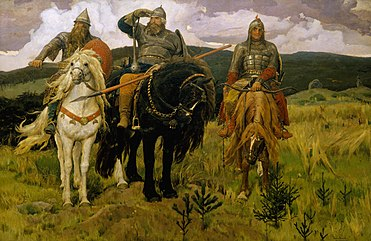
\includegraphics[width=0.49\textwidth]{img/tri_bogatyrya.jpg}
    \end{center}
    \caption{Картина «Три Богатыря» ВМ Васнец\'{о}ва (слева направо: Добрыня Никитич, Илья Муромец и Алёша Попович), ВикипедиЯ.}
\end{wrapfigure}
В центре картины изображён Илья Муромец, народный любимец, герой русских был\'{и}н. Не всем известно, что Илья Муромец не сказочный персонаж, а реальное историческое лицо. История его жизни и \explainDetail{р\'{а}тных}{р\'{а}тный}{military} \explainDetail{п\'{о}двигов}{п\'{о}двиг}{exploit, feat} -- это реальные события. \explain{Впосл\'{е}дствии}{subsequently}, закончив свои труды по охране родины, он стал монахом Киево-Печёрского монастыр\'{я}. Был причислен к л\'{и}ку свят\'{ы}х\footnote{was canonised}. Васнецов эти факты знал, создав\'{а}я образ Ильи Муромца. «\explainDetail{Матёр}{матёрый}{mature, fully grown, hardened} человек Илья Муромец» -- говорит былина. А на картине Васнецова мы видим могучего воина и при том \explainDetail{бесх\'{и}тростного}{бесх\'{и}тростный}{ingenuous, silly} открытого человека. В нём \explainDetail{сочетаются}{сочетаться}{combine} исполинская сила и \explain{великод\'{у}шие}{generosity, magnanimity, goodness}. «А конь под Ильёй \explain{лютый}{fierce} зверь» -- продолжает сказание. \explainDetail{Мощная}{мощный/-ая/-ое}{powerful} фигура коня, изображённого на картине с массивной металлической цепью вместо упряжки, \explainDetail{свид\'{е}тельствует}{свид\'{е}тельствовать}{testify; свидетель: witness} об этом.

Добрыня Никитич по народным преданиям был очень образ\'{о}ванным и \explainDetail{м\'{у}жественным}{м\'{у}жественный}{manly} человеком. С его личностью связано много чудес, наприм\'{е}р, заговорённая броня\footnote{charmed armor} на его плечах, \explain{волш\'{е}бный}{magic} меч-кладенец. Добрыня изображён таким как и в былинах -- величавым, с тонкими, благородными чертами лица, подчёркивающими его культурность, образ\'{о}ванность, \explain{решительно}{decisively} вынимающий меч из \explain{н\'{о}жен}{sheath} с готовностью \explainDetail{бр\'{о}ситься}{брос\'{а}ться/бр\'{о}ситься}{rush} в бой, защищая свою родину.

Алёша Попович \explain{по сравнению с}{as compared with} товарищами молод и строен. Он изображён с \explainDetail{л\'{у}ком}{лук}{bow} и стрелами в руках, но \explain{прикреплённые}{attached} к \explainDetail{седлу}{седло}{saddle} гусли свидетельствуют о том, что он не только бесстрашный воин, но и \explain{гусляр}{player of the musical instrument ``gusli''}, песенник, весельчак. В картине много таких деталей, которые характеризуют образы её персонажей.

Упряжки коней, одежда, амуниция не \explainDetail{вымышленные}{в\'{ы}мышленный/-ая/-ое}{imaginary, fictitious}. Такие образц\'{ы} художник видел в музеях и читал их описания в исторической литературе. Художник \explain{мастерски}{masterfully} передаёт состояние природы, как бы предвещающей о наступлении опасности. Но богатыри представляют собой \explainDetail{надёжную}{надёжный/-ая/-ое}{reliable} и мощную силу защитников родной земли.




\subsection{Картина «Алёнушка» ВМ Васнец\'{о}ва}
% https://muzei-mira.com/kartini_russkih_hudojnikov/1321-opisanie-kartiny-bogatyri-tri-bogatyrya-vasnecova-1898.html

Алёнушка, печальная девочка у \explainDetail{пруда}{пруд}{pond} --- одна из любимых всеми картин В. Васнецова. Художник уд\'{а}чно использует сказочный сюжет, чтобы \explainDetail{раскрыть}{раскрывать/раскрыть}{to open/to discover} сложный и неоднозначный русский характер.

\begin{wrapfigure}{l}{0.4\textwidth}
    \begin{center}
        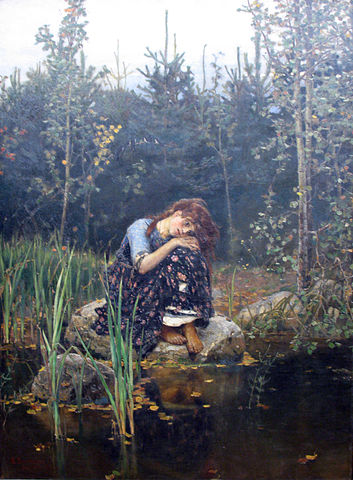
\includegraphics[width=0.38\textwidth]{img/alyonushka.jpg}
    \end{center}
    \caption{Алёнушка, ВикипедиЯ}
\end{wrapfigure}
Грусть девочки очень взрослая. Печаль в её глазах граничит с \explainDetail{отчаянием}{отч\'{а}яние}{despair}. Неубранные рыжие волосы, тёмные глаза, нежно-алые губы --- формируют легко читаемый образ ребёнка с тр\'{у}дной судьб\'{о}й.
В Алёнушке совсем нет ничего \explainDetail{сказочного}{сказочный}{fabulous, fairytale-like}, фантастического.
С\'{о}бственно, вся ск\'{а}зочность сюжета подчеркнута лишь одной деталью --- группой \explainDetail{ласточек}{л\'{а}сточка}{swallow}, сидящих над головой \explainDetail{героини}{героиня}{heroine}. Этим с\'{и}мволом (как известно, л\'{а}сточки символиз\'{и}руют над\'{е}жду) художник \explainDetail{уравновешивает}{уравновешивать/уравновесить}{to balance --- уравнов\'{е}шиваю/-ешь/-ют; уравнов\'{е}шу/-ишь/-ят} полный \explainDetail{тоск\'{и}}{тоск\'{а}}{yearning, longing} \'{о}браз героини, даёт надежду на счастливый финал старой русской сказки.

Васнецов нап\'{о}лнил \explain{ф\'{о}новый}{background} пейзаж атмосферой тишины и гр\'{у}сти.
Отлично удал\'{и}сь художнику в\'{о}дная \explain{гладь}{smooth surface} пруда, \explainDetail{камыш\'{и}}{камыш}{reed}, осока, \explainDetail{ели}{ель}{fir tree}.
Всё \explainDetail{неподв\'{и}жно}{неподв\'{и}жный/-ая/-ое}{still, motionless}, тихо, спокойно.
Даже пруд отраж\'{а}ет героиню очень деликатно, \explain{слегк\'{а}}{slightly}.
Чуть трепещут молодые \explainDetail{ос\'{и}ны}{ос\'{и}на}{aspen}. \explainDetail{Едва}{едв\'{а}}{barely, hardly} \explain{хмурится}{turns gloomly} ос\'{е}ннее небо.
Тёмные, зелёные тона пейзажа контрастируют с \explainDetail{румянцем}{румянец}{blush} на лице героини, а ос\'{е}нняя грусть --- с яркими цветами на юбке Алёнушки. Зритель чувствует: ещё мгнов\'{е}ние и сказка прод\'{о}лжится\dots







\subsection{Картина «Витязь на распутье»}

Виктор Михайлович Васнецов с циклом работ, \explain{посвященных}{dedicated (посвященный + \textit{дат.})} сюжетам русских сказок и былин, оказался \explainDetail{новатором}{новатор}{innovator} в этой области \explainDetail{изобразительного искусства}{изобраз\'{и}тельное искусство}{visual art}. За ним закрепилась репутация «художника-сказочника», он настолько проникся духом русской старины и былинного времени, что свой московский дом построил в виде деревянной избы (сейчас там находится мемориальный музей \explainDetail{живоп\'{и}сца}{живоп\'{и}сец}{painter, artist}).


Картина «В\'{и}тязь на расп\'{у}тье» \explain{отч\'{а}сти}{partly} является и отражением судьбы Васнецова.
Будучи \explainDetail{пр\'{и}знанным}{пр\'{и}знанный}{recognised} художником-передвижником, он, как и его товарищи, \explainDetail{исполнял}{исполнять/исполнить}{performed} жанровые композиции в духе остросоциальных тем, волновавших общество в 1870-1890-х.
Но завладевшая им сказочная тематика диктовала \explainDetail{ин\'{о}е}{ин\'{о}й/ин\'{а}я/ин\'{о}е}{(определительное местоимение) другой, отличный от данного; (неопределённое местоимение) некоторый. See \href{https://ru.wiktionary.org/wiki/\%D0\%B8\%D0\%BD\%D0\%BE\%D0\%B9}{wikictionary.org:иной}.} развитие творчества. Живописец уход\'{и}л от проблем современности и \explain{погружался}{plunge, dive} в мир русской старины, рискуя быть \explainDetail{осужденным}{осужденный}{convicted}.

\begin{wrapfigure}{l}{0.58\textwidth}
    \begin{center}
        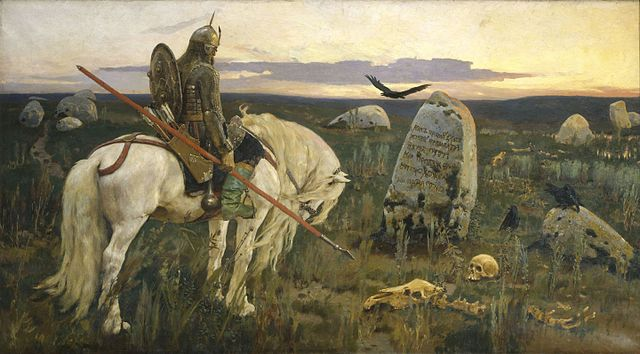
\includegraphics[width=0.57\textwidth]{img/TheKnightAtTheCrossroads.jpg}
    \end{center}
    \caption{Витязь на распутье, ВикипедиЯ}
\end{wrapfigure}
Выбор пути как один из \explain{роков\'{ы}х}{fatal} вопросов человеческой жизни на крупноформатном \explainDetail{холсте}{холст}{canvas} мастера приобрел эпическое звучание.
Перед камнем-предсказателем согнулся под тяжестью фатального \explainDetail{пророчества}{пророчество}{prophecy} опечаленный витязь. \explainDetail{Зловещий}{зловещий}{sinister} в\'{о}рон, садящееся красное солнце нагнетают\footnote{build up the atmosphere} атмосферу. \explainDetail{Нам\'{е}ренный}{нам\'{е}ренный}{intentional} отказ от \explainDetail{изображения}{изображение}{depiction} дороги (как выхода из трудности) художником сделан для того, чтобы показать \explain{неотврат\'{и}мость}{inevitability} судьбы.
\chapter{Мода}

\section{Как мода влияет на нашу жизнь?}

\textit{Источник: \url{https://absurdu.net/fashion/kak-moda-vliyaet-na-nashu-zhizn.html}}

С развитием современных технологий, соцсетей и рекламы большинство из нас осознает, что в той или иной мере мы таки поддаемся определенным трендам и модным тенденциям. И все же, существует немало тех, кто категорически не согласен с этим утверждением. Такие люди утверждают, будто бы мода никоем образом не влияет на их жизнь и, тем более, на поведение. Но так ли это на самом деле? Давайте разбираться!

\textbf{Отражает мировые события и общий настрой людей}

Ни для кого не секрет, что мода всегда отражает культурные, социальные, политические, экономические и религиозные аспекты общества. Если в мире происходит что-то масштабное, это в любом случае тем или иным образом повлияет на fashion-индустрию. Так формируются определенные тренды. Яркое доказательство этому – тенденции 2021 года. Психологи говорят о том, что при возникновении неприятных событий человек нуждается в том, что могло бы положительным образом повлиять на его настроение. Этот принцип находит свое отражение и в модной индустрии. После пандемии и локдауна многие чувствуют усталость и подавленность. Дизайнеры, ощущая потребности своих клиентов, начали создавать более комфортную, но в то же время креативную одежду: мода понемногу отходит от нейтральных оттенков и непрактичных вещей, наоборот, повседневные предметы гардероба становятся более удобными, а палитра цветов гораздо ярче. Насыщенные цвета радуги положительным образом влияют на наше самоощущение и восприятие мира, а интересные фасоны, асимметрия или архитектурный крой в одежде смотрятся нарядно и элегантно, что способствует ощущению воодушевленности и праздничного настроения.

К интересным выводам пришли также те, кто занимается изучением истории fashion-индустрии. После масштабных войн или экономических кризисов одежда становилась все более откровенной. Фасоны прилегали к телу, подолы юбок и платьев укорачивались. С одной стороны, это было связано с практичностью, а с другой – с банальной нехваткой материалов. Из-за тяжелого положения в такие времена люди просто не могли тратить по 40 метров ткани на одно платье!
То же самое можно сказать и про сферу религии и морали. Все знают, что в мусульманских странах девушки не могут носить одежду, которая бы открывала их шею, запястья или щиколотки. Поэтому мода в таких государствах обычно гораздо более консервативная, но все же поддается изменениям. Тем более, что под хиджабом или паранджей женщина может носить то, что нравится ей, если это соответствует принципам одежды, записанным в Коране. Кроме того, в большинстве случаев они не ограничены в выборе аксессуаров. Так, например, во всемирно известном торговом центре Dubai Mall в ОАЭ, куда съезжаются люди из всех уголков мира, довольно часто можно встретить пару, в которой супруга идет в лодочках от любимого люксового бренда, а руках у нее оригинальная сумка Chanel или Dior.

\textbf{Продвигает инклюзивность, меняет представление о красоте}

Конечно, представление о «красоте» очень субъективное, но, тем не менее, наше восприятие этого абстрактного понятия в огромной мере зависит именно от «канонов» fashion-индустрии. До 70-80-х прошлого века люди не сильно обращали внимание, на то, как выглядит их тело. Но с популяризацией спорта и развитием некоторых его видов в моду приходит «культ тела», подразумевающий подтянутую спортивную фигуру не только у мужчин, но также и у женщин. Вспомните также, как менялось представление об идеальных модельных параметрах: в 2000-е годы большинство представительниц этой профессии имели явно нездоровый вид, что чаще всего было следствием анорексии. Со временем, когда суровый fashion-мир наконец-то переосмыслил понятие красоты и здоровья, на подиумы стали выходить модели плюс-сайз. То же самое касается и темнокожих девушек: еще в конце прошлого века для большинства из них принять участие в показе или появиться на обложке глянца казалось недостижимой целью, а сегодня вопрос происхождения не является препятствием при построении карьеры. Если говорить об особенностях, как, например, кожа супермодели Винни Харлоу или страбизм (косоглазие) Брунетт Моффи, все больше людей также перестают обращать на это внимание.

Выпускники Лондонского колледжа моды Джудит Ахумба-Велленстайн, Сьюзан Джин и Пак Лунчиу, которые создали онлайн-журнал Hajinsky, посвященный фэшн-психологии, изучив то, какое воздействие мода имеет на жизнь большинства людей, пришли к следующему выводу:

\begin{fancyquotes}
    «Официальная одежда положительно влияет на абстрактное мышление человека, которое связано с такими действиями, как, например, экономия денег. Кроме того, наука показала, как бренды могут улучшить жизнь общества, сделав одежду инклюзивной. Исследования показали, что люди с ограниченными физическими возможностями часто для удобства носят спортивные костюмы и поэтому подвергаются двойной дискриминации — во-первых, из-за своей физических особенностей, во-вторых, из-за своей одежды. Бренды, принимающие это во внимание, могут в корне изменить жизнь человека».
\end{fancyquotes}

\textbf{Исполняет роль идентификатора личности}

Мода также помогает нам больше понять других и служит неким идентификатором. Например, по национальному костюму мы можем догадаться, из какой страны человек, общий внешний вид иногда указывает на род деятельности, а характерная манера сочетать вещи может служить неким маркером «творчества», «вкуса» и т.д. Те же, кто все еще категорически отказываются принимать факт влияния моды на их жизнь, не могут отрицать того, что в современном мире просто нельзя избежать ситуаций, когда мы должны выглядеть определенным образом. Представьте, что вас пригласили на свадьбу, на торжественный ужин в дорогой ресторан или же вы идете на собеседование в крупное финансовое учреждение с наличием определенного дресс-кода. Для такой ситуации вы вряд ли наденете джинсы. Для подобных случаев существует различные наряды, в том числе классический деловой костюм, который так же пришел в нашу жизнь под влиянием определенных тенденций. Нельзя отрицать тот факт, что внешний вид человека также сказывается на том, как другие воспринимают его. Именно по этой причине мы часто задумываемся о том, какую одежду подбирать не только под определенную ситуацию, но даже под сам круг общения. Наше естественное желание нравиться способствует тому, что время от времени мы обновляем свой гардероб и добавляем туда красивые (которые соответствуют нашему субъективному вкусу) предметы одежды и аксессуаров.

\begin{fancyquotes}
    «Реальность такова, что мода стала частью нашей повседневной жизни. Она связана с политикой и может вызвать социальные перемеФормирует сознаниены. Мода также влияет на наши отношения друг с другом, наше поведение, она может улучшить нашу жизнь, помогая с самоидентификацией»,- заявили вышеупомянутые основатели журнала Hajinsky.
\end{fancyquotes}

\textbf{Формирует сознание}

И это касается даже тех, кто никогда не следит за ней. Если все начинают носить оверсайз, со временем при покупке новой футболки вы также сделаете выбор в пользу прямого или более свободного фасона. Кроме того, это отражается и в количестве покупаемых предметов. Сейчас большинство людей приобретают намного больше одежды, обуви и аксессуаров, чем это было еще 30 лет назад.

\begin{fancyquotes}
    «При выборе гардероба важно ориентироваться на свои ценности и цели. При этом человек не может существовать в полном отрыве от общества. В этом смысле, если „психология моды“ про гармонизацию запросов общества и внутренних процессов человека, то это может повысить качество его жизни». – Говорит психолог Александра Меньшикова.
\end{fancyquotes}

Также нельзя забывать, что мода – это не только об одежде. Поэтому если вы не следуете трендам при формировании своего гардероба, это не значит, что вы не изучите последние тенденции, когда, например, будете делать ремонт в квартире. То же самое касается приобретения новой техники, автомобиля или даже посуды на кухню.

Хотите вы того или нет, мода в любом случае влияет на ваш выбор повседневных образов, домашней обстановки и даже места для отдыха. И это нельзя определить как «хорошо» или «плохо» — каждый оценивает по-своему. Остается лишь принять тот факт, что мода в большой степени влияет на разные сферы нашей жизни, а вот активно следовать новым тенденциям, принимать их или всеми силами пытаться убежать от них – личное дело каждого. Но, согласитесь, знание — сила. Осознанность поможет вам разумно подходить к вопросу трендов и тенденций, чтобы умело использовать этот инструмент для достижения своих целей. Актуальный и стильный внешний вид еще никому не помешал.
\chapter{Досуг}

\section{Моё хобби}
У каждого человека свои предпочтения --- «На вкус и цвет товарищей нет». Каждый из нас увлечен занятиями, которые мы выбираем согласно нашим пожеланиям. Кому-то нравится заниматься спортом, а кому-то нет. Кто-то бы с удовольствием заняться \explain{вышиванием}{вышивание: embroidery}, а для кого-то вышивание --- это нудное и скучное занятие.
Вот, например, я очень люблю коллекционировать различные безделушки и сувениры. Это занятие очень увлекает меня и я от него в восторге. Еще я обожаю писать стихи, рисовать и читать. Больше всех я люблю читать детективы.

Моя двоюродная сестра ненавидит сидеть дома. Ей больше нравится активный образ жизни. Нед\'{а}вно она начала заниматься теннисом. \explain{В общем и целом}{in general}, в свободную минуту она \explain{не прочь}{is not averse to} спеть какую-нибудь иностранную песню на французском языке. Она просто обожает французский язык, традиции и обычаи французов. В будущем она планирует нанести визит во Францию и зайти в гости к своей тете, которая уже как 10 лет там живет.

Мой старший брат без ума от машин. Он коллекционирует старые машины, реставрируя их на свой стиль. \explain{Помимо всего}{Besides (all)}, он еще и очень спортивный парень. Три раза в неделю он ходит в спортзал и занимается там по 2-3 часа. Я же ненавижу спорт. \explain{Умственные}{intellectual} упражнения для меня важнее, чем физические. Но мой брат думает \explain{по-другому}{otherwise}. Он \explain{придерживается}{adheres to/sustains} позиции: «В здоровом теле здоровый дух».
\chapter{Карьера и профессии}

\section{Устройство на работу}
Закончив университет и получив диплом юриста, я решил начать искать подходящую по специальности работу.

К сожалению, у меня сразу не получилось занять высокий пост.
Все как в один голос твердили, что у меня недостаточно практики, поэтому сначала н\'{у}жно получить практические знания и поработать несколько месяцев стажером.

Я так и сделал.
Посетив одну фирму в обрабатывающей промышленности, мне очень понравился не только коллектив и месторасположение компании, но и уровень заработной платы и перспектива роста.
Именно поэтому я принял для себя решение получить эту работу, чего бы мне это ни стоило.
Как оказалось, что сделать это было не так-то просто.

Сначала н\'{у}жно было поработать один месяц бесплатно, а потом целых три месяца стажером.
Работая стажером, я получал 30\% от зарплаты.

Эта сумма не была велико, но в то же время мне хватало этих денег на еду, оплату коммунальных услуг и на простые развлечения.

По происшествии 2 месяцев, работодатель заметил мое трудолюбие и талант, поэтому повысил мне зарплату еще на 20\%.

Я был безумно рад этому событию. Прошло 4 месяца и мне предложили полную ставку.
Для этого я заполнил анкету, прошел тест и ознакомился с новыми условиями работы.

К счастью, они были очень выгодными --- премии, надбавки за сверхурочные, оплачиваемый отпуск и оплачиваемые праздничные дни.

Я был на седьмом небе от счастья от такого предложения!

\section{Устройство на работу (2)}
Source: \href{http://irkzan.ru/home/gragd/soiskatel/soiskatelrabota.aspx}{Министерство труда и занятости иркутской области}.

Как начать поиск \explain{подходящего}{suitable} места работы? Как найти интересную работу и одержать победу в конкуренции с другими кандидатами? Для ответа на эти вопросы необходимо помнить:

\begin{itemize}[noitemsep, label=--]
    \item процесс поиска работы Вы должны взять в свои руки, \explain{проявляя}{exhibiting; showing} активность и инициативу;
    \item не ограничивайтесь одной специальностью, составьте список работ, который Вы можете выполнять;
    \item \explain{если Вы определили}{if you have identified} для себя какую работу вы ищете, рассказывайте об этом всем вокруг. Чем больше людей знают об этом, тем лучше;
    \item занимайтесь поиском работы 8 часов в день, считая это свой работой;
    \item работодатели стремятся \explain{нанимать}{to hire} победителей. Будьте уверены в себе, умейте подать себя;
    \item \explain{настройтесь}{tune in (to the fact)} на то, что Вы можете получить десятки \explainDetail{отказов}{отказ}{failure} --- это нормально;
    \item \explain{очередной}{next; following} отказ не должен выбивать Вас из колеи, а наоборот, пробуждать к дальнейшему поиску работы.
\end{itemize}

Современный рынок труда очень специфичен. Каждая сторона --- продавец и покупатель --- старается создать ситуацию выбора для себя: специалист, решивший сменить работу, как правило, \explain{рассматривает}{considers} несколько \explainDetail{предложений}{предложение}{offer} от работодателей, несколько вариантов работы, чтобы выбрать те \explain{условия}{conditions} работы, которые его больше \explain{устраивают}{satisfy} и, одновременно --- продать себя как можно дороже. Работодатель также проводит тщ\'{а}тельный отб\'{о}р кандидатов на рабочее место, чтобы \explain{приобрести}{to acquire} товар как можно лучшего качества и как можно дешевле.

Прежде всего, необходимо установить контакты с рынком труда, поскольку работодатель сам не придет к Вам со своими предложениями. Заставьте информацию работать на себя. Расскажите о том, что Вы ищете работу сослуживцам, родственникам, знакомым, соседям, бывшим одноклассникам и однокурсникам, преподавателям и администраторам учебных заведений, в которых Вы учились и др.

Стоит заглянуть в раздел объявлений в газетах. Прежде всего, обратите внимание на объявления тех фирм, которые указывают свое название, а не выступают обезличенно, скрываясь за абонентным ящиком или ничего не говорящим «организации требуются». Зная, о какой фирме идет речь, Вы можете навести о ней справки и потом решать, стоит ли пытаться попасть в нее. Ни для кого не секрет, что благополучные предприятия не нуждаются в рекламе, и люди, приходят на них сами, чаще всего по рекомендации. Адреса таких предприятий можно взять из специализированных журналов, отраслевой справочной литературы, наконец, просто из телефонных справочников.

Следующим этапом поиска может стать «прозвон» газетных предложений. При общении с работодателем необходимо:

быть вежливым, голос должен быть уверенным;
рядом иметь ручку и листок бумаги для записи необходимой информации;
отвечать на вопросы быстро и кратко, договориться о встрече.

\subsection{Резюме и его роль в трудоустройстве}
Грамотно составленное резюме демонстрирует умение излагать свои мысли на бумаге, умение оценить себя, умение исполнять предстоящие условия и работу. С помощью резюме можно информировать максимальное число работодателей о себе как о претенденте на вакантные рабочие места.

Правила составления резюме:

\begin{itemize}[noitemsep, label=--]
    \item резюме должно быть кратким (не более двух страниц);
    \item резюме должно включать только ту информацию, которая является значимой для работодателя;
    \item старайтесь не использовать сокращений.
\end{itemize}

Следует обязательно указать:

\begin{enumerate}[noitemsep]
    \item \textit{Ф.И.О.}, домашний адрес, контактный телефон. (Резюме, содержащие только адрес электронной почты, обычно не рассматриваются.
    \item \textit{Цель}. Название позиции на которую претендуете. Укажите должность, на которую Вы претендуете. Бывает, что соискатели указывают сразу несколько возможных вариантов трудоустройства, когда варианты имеют близкие функциональные обязанности. Например: «Ищу работу секретаря-референта, офис-менеджера, менеджера по работе с клиентами».
    \item \textit{Образование}. Необходимо указать полностью название учебного заведения, дату поступления и его окончания, специальность. Если высшее образование уже получено, не стоит упоминать о дате окончания средней школы. Если Вы получили дополнительное образование (закончили курсы, прошли тренинги), не перечисляйте все подряд, а только то, что имеет непосредственное отношение к профессии.
    \item \textit{Опыт работы}. Необходимо указать дату поступления и окончания работы, наименование организации, профиль ее деятельности, название должности и краткое описание должностных обязанностей и достижений в хронологическом порядке, начиная с последнего места работы.
    \item \textit{Профессиональные навыки}. В графе указывается знание и степень владения иностранными языками, знание специальных компьютерных программ текстовых редакторов, наличие водительских прав.
    \item \textit{Дополнительная информация}. В графе указывается наличие загранпаспорта, наиболее сильные черты характера и т.д.
    \item Укажите на возможность предоставления рекомендаций.
    \item Вся информация, содержащаяся в резюме, обязательно должна быть достоверной.
\end{enumerate}

\subsection{Пример резюме}
Петров Владимир Петрович

663000 г. Иркутск, ул. Российская,82 кв 16 тел. 33-56-78

\textbf{Цель}: Получение должности коммерческого директора в торговой компании

\textbf{Образование}:

\begin{itemize}[noitemsep, label=--]
    \item 1990-1995 Иркутская государственная экономическая академия. Инженерно-экономический факультет. Диплом инженера-экономиста
    \item 1996-1997 Курсы английского языка при Лингвистическом университете.
    \item 1998 Курсы по маркетингу при учебном центре ИГЭА
\end{itemize}


\textbf{Опыт работы}:

\begin{itemize}[noitemsep, label=--]
    \item 3.1998 --- н/время Фирма «Плюс» (Россия г. Иркутск) начальник отдела продаж.
          Оптовая торговля продовольственными товарами
          (консервы, сухие супы)\\
          Функции: организация продаж, контакты с розничными
          торговыми предприятиями, составление договоров, контроль за
          расчетами. В подчинении 3 человека. За период работы
          расширил сеть торговых точек с 17 до 60.


    \item 8.1995 --- 3.1998 ИЧП «ФОБОС», коммерческий агент.
          Розничная торговля продовольствием и ТНП.\\
          Функции: реализация товара через торговые точки фирмы.
          В 1996 г оборот фирмы достигал 3,5млн. руб. в год
\end{itemize}




\textbf{Дополнительные сведения}:
\begin{itemize}[noitemsep, label=--]
    \item Английский язык (могу изъясняться и работать с профессиональной документацией)
    \item РС --- пользователь (WinWord, Exel). Водительские права кат.В Опыт вождения 4 года. Имеется личный автомобиль.
\end{itemize}




% ----
\subsection{Собеседование с работодателем}
Пришел положительный ответ с предложением явиться на собеседование. Теперь главное --- произвести хорошее впечатление.

\textbf{Подготовка к собеседованию}.

А) Предоставляемые документы

В большой степени решающим для достижения успеха в поисках работы имеют внешний вид предоставляемых документов. Испачканные или порванные документы заставляют читающего их человека предположить, что кандидат в работе также неряшлив и несобран.

Для руководителя отдела кадров, как показывает практика, важнейшим документом, который помогает быстро ознакомиться с личностью кандидата, является автобиография, которая должна быть отпечатана на машинке.

В настоящее время все большее число фирм требует от кандидатов на должность, наряду с другими документами, заполненную личную анкету, которая смогла бы дать ответы на все вопросы, связанные с его первичной оценкой. Специфические условия каждой фирмы заставляют их включать в анкету соответствующие этим условиям вопросы. Фирма придает различное значение тем или иным качествам кандидатов, что и находит отражение в содержании анкеты. Содержание анкеты определяет также постоянно меняющееся положение на рынке труда.

Б) Внешний вид

Оденьтесь так, чтобы Вам было прежде всего удобно и Вы чувствовали бы себя свободно и уверенно, а не как на торжественном приеме у английской королевы. Женщины не должны усердствовать по части косметики и украшений. Не рекомендуется также одевать короткие и узкие юбки и платья и выбирать духи с «навязчивым» ароматом. Тоже самое относится и к мужчинам в отношении лосьона после бритья. Костюм и рубашка должны гармонировать по цвету. Если Ваша работа предполагает наличие у Вас «легкости на подъем», частые поездки и вообще подвижность, можно выбрать для этой встречи спортивный стиль одежды: приличного вида свитер или джемпер с выпущенным воротничком свежей сорочки, спортивного покроя брюки или джинсы, легкая обувь. Не следует путать спортивный стиль со спортивной одеждой. И в Москве, и в Иркутске нередко можно встретить молодых людей, носящих «мастерку» с пиджаком, спортивный костюм в комбинации с рубашкой, галстуком и кожаными туфлями. Нелепо будет выглядеть мужчина, пришедший устраиваться в спортивном костюме даже фирмы «Адидас». Мнение, что цена костюма придает ему солидность, глубоко ошибочно.

До собеседования:
\begin{enumerate}[noitemsep]
    \item проверьте время, дату и путь;
    \item исследуйте компанию;
    \item отрепетируйте вопросы и ответы;
    \item подумайте, что вы оденете и как будете выглядеть
\end{enumerate}



% ----------
\subsection{Пять первых критических минут}
Много кандидатур на разные работы отвергают в течение первых пяти минут собеседования.

Критический момент наступает, когда Вы входите --- в Вашем внешнем виде не должно быть ничего, что может вызвать разочарование.

Лучший первоначальный подход --- это улыбнуться. Это неизменно побуждает дружелюбные чувства в человеке, улыбка дает нам почувствовать себя намного лучше и более уверенно.

Другие полезные подсказки, которые следует использовать в первые пять минут:

не выкладывайте ничего, что принесли с собой до того, как собеседник предложит Вам сделать это;
предоставьте собеседнику возможность первому протянуть Вам руку для рукопожатия;
не садитесь, пока Вам не предложат.


\textbf{Поза.}
Устройтесь удобно, сядьте прямо, но без \explain{напряжения}{напряжение}{stress; tension; voltage}.
Не облокачивайтесь и не кладите руки на стол собеседника.
Не разваливайтесь на стуле.
Вы будете выглядеть куда более представительно, сидя прямо, нога на ногу, ваши руки расслабленно лежат на коленях. Неплохо убедиться, что ваш стул отодвинут от стола собеседника, чтобы дать Вам свободу движений.


\subsection{Получение информации}
Собеседование проводится для того, чтобы обе стороны давали и получали информацию. Одна из главных установок --- получить всю нужную вам информацию о работе и самой организации. Никогда не соглашайтесь на работу, пока не убедитесь, что она Вам подходит.

Не надо:
\begin{enumerate}[noitemsep]
    \item извиняться за свой возраст, здоровье, недостаток опыта;
    \item перебивать собеседника;
    \item критиковать последнего работодателя;
    \item быть слишком фамильярным или самоуверенным;
    \item шутить, ругаться или курить.
    \item Типичные вопросы работодателей при приеме на работу
\end{enumerate}


Почему Вы хотите здесь работать?
\begin{enumerate}[noitemsep]
    \item Выполняли ли вы работу такого рода раньше?
    \item Что Вы делали с тех пор, как стали безработным?
    \item Почему Вы ушли с последнего места работы?
    \item Почему Вы так долго оставались без работы?
    \item Как долго вы намерены работать у нас?
    \item Чем Вы занимались на последнем месте работы?
    \item На каком оборудовании Вы работали?
    \item В чем заключаются Ваши сильные стороны?
    \item Каковы Ваши слабые стороны?
    \item Расскажите нам побольше о себе?
    \item Какую зарплату Вы хотели бы получать?
    \item Были ли у вас конфликтные ситуации на работе?
    \item Когда вы сможете приступить к работе?
    \item Каким образом Вы планируете добираться до работы вовремя?
    \item Есть ли у Вас какие-либо вопросы?
\end{enumerate}

После собеседования:
\begin{enumerate}[noitemsep]
    \item поблагодарите компанию за собеседование в кратком письме;
    \item если от работодателя не будет вестей, то позвоните и спросите, каков результат собеседования.
\end{enumerate}

Помните! В каждом из Вас есть внутренние резервы. Используйте их. Разбудите свою активность --- и успех будет в Ваших руках.

Желаем скорейшего трудоустройства!


\section{Виртуальный ассистент: профессия будущего}
Source: \href{http://www.cyprusmoms.com/virtualnyj-assistent-professiya-budushchego/}{www.cyprusmoms.com}.\\

Представьте ситуацию: вы живёте в стране, в которой не имеете возможности работать. Дети подрастают, хочется реализоваться профессионально, но идей для собственного бизнеса нет, да и времени свободного всего час-два в день. Знакомо?

Думаю, что я не одинока в таком положении. Живу на Кипре уже давн\'{о}, но разрешения на работу нет, да и найти работу в нашей деревне довольно сложно. Поэтому я начала думать об \explainDetail{удалённой}{удалённый/-ая}{remote} работе через интернет --- \explainDetail{вела}{вести/повести (веду, ведёшь, ведут)}{to lead} собственный блог, администрировала несколько групп в Фейсбуке для поддержки местного комьюнити, писала статьи, фотографировала, но не понимала, как перевести это хобби в \explainDetail{опл\'{а}чиваемую}{опл\'{а}чиваемый}{paid (from: оплачивать/оплатить)} деятельность.

Да, я читала рекламные статьи школ, которые онлайн обучают различным профессиям, но мне было непонятно, как потом находить работу, как работать с клиентами, чем \explain{зацепить}{to hook on; to catch (цепь: chain)} клиента, когда на рынке множество таких \explainDetail{новичков}{новичок}{newbie}, как я...

И вот, когда некоторое время назад я прочитала статью о профессии «Виртуальный ассистент», во мне щёлкнуло --- вот оно! То дело, которое я искала.

Кто такой виртуальный ассистент? Это универсальный специалист, который помогает предпринимателю вести бизнес в интернете --- наполняет страницы в социальных сетях, верстает лендинги и презентации, организовывает вебинары и налаживает \explainDetail{почтовую рассылку}{почтовая рассылка}{mailing list}.

В зависимости от предыдущего опыта, ассистент может специализироваться в том или ином направлении. Но в целом, это человек, который хорошо ориентируется в интернете, может найти нужный сервис, написать запрос, проконтролировать подрядчиков и быть тем многоруким многостаночником, который снимет с предпринимателя рутинные обязанности. И не важно, в какой стране живёт предприниматель и какое гражданство имеет Виртуальный ассистент --- они встречаются и сотрудничают в интернете.

{\it К 2020 году 20\% рабочих мест в России будут виртуальными, сказано в исследовании «J’son \& Partners Consulting», сделанном по заказу сервиса «Битрикс24». По данным исследований 2016 года эта цифра в Европе составляет 17\%, а в Японии и США доходит до 40\% от всех работающих.}

Я погуглила и поняла, что в англоязычной среде эта профессия очень распространена, даже существуют ассоциации бизнес-помощников.
На русскоязычном пространстве информации меньше, но есть несколько школ подготовки виртуальных ассистентов.
И все они --- что очень ценно --- обещают помощь со стажировками и трудоустройством. Результаты исследования школ, которые готовят бизнес-помощников, вы можете посмотреть на моей странице в фейсбуке Я остановилась на Международной школе подготовки бизнес-ассистентов и интернет-маркетологов «Helppy» Ольги Шевченко и ни минуты не пожалела. И организация обучения, и полезность информации --- на высоте!

Обучение длится пять недель, и погружение в учебу полное. За 35 дней ты вникаешь в принципы организации интернет-бизнеса, верстаешь презентацию в Пауэр Поинт, составляешь контент-план и график постов в рамках тобой же разработанной стратегии продвижения в соцсетях, верстаешь лендинг --- одностраничный сайт, а так же --- ТА-ДАМ! --- составляешь портфолио для самого себя. Понятно, что это не все темы, а только те, по которым требовалось сдать домашнее задание, и над которым мы все корпели ночами. На все домашки ты получаешь развёрнутые ответы, и очень редко удавалось сдать их с первого раза, спрашивали очень строго --- то типографика хромает, то дизайн подвёл.

Кроме лекций и обучающего материала, в закрытом разделе собрана база данных полезных статей, в секретной группе кипит жизнь --- кураторы и сокурсники обсуждают задания, а по пятницам Ольга Шевченко разговаривает с каждым курсистом отдельно и отвечает на все волнующие вопросы.

Создание портфолио --- это огромный пендаль собственной самооценке. После того, как ты соберешь всё, что ты можешь, применишь правила сильного текста, прикрутишь туда отзывы клиентов (мы делали домашнее задание по заказу интернет-предпринимателей, а они нам писали отзывы), подберёшь шрифты, а потом ещё сверстаешь это в лендинг с красивыми картинками... От этогосамооценка лезет вверх, и ты готова на подвиги и новые свершения. Хотите посмотреть на моё портфолио?Здесь. Я вам его показываю не для того, чтобы похвастаться, а для того, чтобы показать, что у вас может получиться на выходе.

Хорошо, что я начала учиться заранее, поэтому даже успевала спать и вести клиентов, которых нашла тут же, рядом с собой. Дело в том, что, начиная заниматься и вникать в тему, у тебя обостряется зрение и ты видишь, что в этом проекте, например, ты можешь быть полезной, а здесь ты можешь докрутить страницу и получить совсем другие результаты. Ты предлагаешь свои услуги, показываешь, что можешь сделать, как можешь помочь, и люди откликаются. Я и многие сокурсники именно так получили работу.

Я не обещаю лёгкой жизни --- учиться и работать надо будет много, информация в интернете меняется быстро, у Фейсбука, например, нововведения каждую неделю, ежедневно на рынок труда выходит всё больше людей. Надо будет выстраивать свой график работы и думать о тайм-менеджменте. Например, черновик этой статьи я набирала на телефоне в гугл-кипе в то время, пока мастер педикюра работала с моими ногами. А от одного, очень перспективного предложения пришлось отказаться, потому что я понимала --- или работа, или семья, третьего не дано, со всем в данный момент не справлюсь.

Профессия виртуального ассистента --- хорошая ступенька для тех, кто выходит из декрета и живёт в том месте, где устроиться на работу сложно. Это профессия для того, кто умеет работать с большим количеством информации и в состоянии организовать рабочие процессы и самого себя. А дальше можно покорять новые вершины, и истории выпускников школы тому подтверждение.

Удачи!

\section{Правила деловой переписки}

\textit{Источник: \url{https://4brain.ru/blog/pravila-delovoj-perepiski/}}

В информационном веке важно обладать умениями и навыками общения в сети Интернет. С одной стороны, письменная речь основывается на тех же правилах, что и устная, с другой, в отдельных направлениях есть необходимость использовать особые приемы, чтобы заочно, не видя собеседника, выстроить с ним правильную коммуникацию и быстрее прийти к нужному результату, используя минимум слов и писем.

Управленцам, менеджерам, редакторам, маркетологам – правила деловой переписки необходимо знать всем. Заинтересовать собеседника, получить результат от взаимодействия с ним можно только при правильном подходе. Стоит учитывать, что при удаленном контакте, когда собеседники не видят друг друга, отсутствует визуальный контакт и возможность использовать множество слов.

В данном случае краткость-сестра таланта – это одно из главных правил продуктивной переписки. Не всегда люди имеют возможность читать длинные письма, поэтому мысли нужно излагать максимально точно и лаконично.

В деловой электронной переписке есть общепринятые правила, грамотно используя которые можно не переживать, что письмо отправится в «Спам». Они подробно изложены в книге создателя сервиса «Главред» Максима Ильяхова «Новые правила деловой переписки», которая считается лучшим пособием в своем роде в России. Соавтор Людмила Сарычева – автор статей о деловом общении.

Опираясь на книгу, мы расскажем о том, как освоить правила деловой переписки, в чем они заключаются и выясним, зачем они вообще нужны, если можно просто излагать свои мысли, чтобы удаленно изъясняться с собеседником.

А чтобы научиться лучше взаимодействовать с людьми и подтянуть или развить навыки общения, рекомендуем пройти нашу программу «Лучшие техники коммуникации». Полученные знания будут полезны в письменной, устной речи, при взаимодействии с коллегами, партнерами и т.д.

\textbf{Типичные ошибки авторов}

Казалось бы, что сложного в том, чтобы написать письмо и, как кажется, договориться с собеседником на расстоянии о чем угодно. В этом как раз кроются типичные ошибки обывателей, чьи письма часто отправляются в «Спам».

На основе материалов, изложенных в книге Максима Ильяхова «Правила деловой переписки», разберем основные проблемы писем, которые буквально лежат на поверхности и видны сразу [М. Ильяхов, 2018]:
\begin{enumerate}
    \item В письме нет темы. Предположим, у адресата большая нагрузка на работе и просматривать почту оперативно он не может. За день на его ящик придет, например, двадцать писем. Каждое нужно прочитать, обработать. Представляете, сколько времени потребуется на чтение? Соответственно заголовок письма обозначит, что внутри, а значит, послужит своеобразным маяком для читающего. Идеальное решение – сделать такой заголовок, который полностью отражает смысл письма. В книге также дана рекомендация помещать в теме такие подробности, которые обозначат, стоит ли читать письмо сразу, какие действия необходимо предпринять для решения вопроса.

    \item «Уважаемые коллеги» --- типовой и очень распространенный шаблон, который, как оказывается, вызывает непонимание и не стимулирует концентрацию силы, а оказывает обратный эффект. Он звучит как «Коллеги, разберитесь сами, кто это сделает», а также не вызывает уважения из-за отсутствия адресата в обращении. Если нужно что-то сделать, решить вопрос, лучше написать конкретному человеку и дать ему подробную информацию, нужные вводные, а не делать коллективную рассылку. Такой подход гораздо эффективнее.

    \item Вторжение в свободное время человека без извинений. «Как проходит выходной / больничный / отпуск?» – эти вопросы точно вызовут раздражение, ведь человек вне рабочего времени занят своими делами. Если возникает острая ситуация, когда участие адресата все же необходимо, важно извиниться за вторжение и обосновать проблему, чтобы человек понял, что задачу решить нужно срочно.

    \item «У меня отличная новость!» По мнению Ильяхова, это дурная фраза, за которой обычно кроется не хорошая, а плохая новость, поэтому лучше сразу переходить к делу, а не создавать вид, что все хорошо.

    \item Абстрактные суждения без постановки конкретной задачи: «Надо бы сделать», «Я тут подумал» и подобные. Людей раздражает неопределенность во всех сферах жизни, в том числе и в постановке задач. Если сотрудник сам будет додумывать детали задачи, он рискует не попасть в мысль того, кто эту самую задачу ставит. В письме должны быть изложены все аспекты вопроса.

\end{enumerate}

Это основные ошибки, которые чаще остальных встречаются в письменной речи обывателей и приводят к медленному решению задач. В книге их перечислено больше: минимум вопросов в одной теме письма, не приложенные файлы, ошибки в обращении, чрезмерное использование шаблонных фраз и стоп-слов. Хочется отослать пишущего к еще одной книге Ильяхова «Пиши, сокращай» – меньше лишних слов, больше четкости и адресности, тогда письмо наверняка будет замечено и прочтено.

\textbf{Что раздражает читателя?}

А теперь поговорим о том, что раздражает читателя делового письма. С отсылкой к «Правилам деловой переписки», книге главреда.

\textbf{Небрежность}

Ошибки пунктуации, неверно составленные предложения, отсутствует подпись. Письма на скорую руку тоже должны быть написаны с умом, иначе получатель может подумать, что задача не первостепенная, раз так небрежно составлена.

\textit{Небрежный текст:} «Здравствуйте Михаил составте пожалуйста список сотрудников для согласования допусков на объект».

\textit{Как надо:} «Добрый день, Михаил! Прошу Вас составить список сотрудников для согласования допусков на объект до 15 января. Директор отдела».

Как видно, в первом предложении есть ошибки орфографии и совсем отсутствуют знаки препинания. Во втором случае просьба оформлена точно, есть обращение, дедлайн, подпись.

\textbf{Панибратство}

Оно выражается в пренебрежительном обращении, например, «народ», «приветик» без соблюдения субординации. Подобное обращение вызывает лишь отторжение, но не самими словами, а нарушением личных границ тех, к кому оно адресовано. Подобное допустимо в неформальной обстановке, но не на работе.

\textbf{Перекладывание ответственности и создание групповых переписок}

В групповых переписках, в которых есть неадресные обращения, никто не понимает, кому полагается решение задачи. Это распространенная проблема в больших коллективах при отсутствии грамотных управленцев.

Как не надо: «Коллеги, нам нужно обсудить вопросы размещения рекламы на сайте партнеров. Какие предложения?»

Как надо: «Сергей, примите решение, стоит ли размещать рекламу у партнеров – обещают 1 млн просмотров. Медиаплан в приложении».

Как идентифицировать сотрудника, который перекладывает ответственность? Он использует такие фразы: «передам коллегам», «это не в моей компетенции», «жду решения руководства». За ними скрывается «сами внесите правки, я в этом не участвую, не трогайте меня».

\textbf{Неуместность фраз и бездумное употребление сокращений}

Случается такое, что отдельные сотрудники используют жаргонизмы и сокращения либо неуместно, т.е. без понимания их смысла, либо настолько часто, что не все коллеги понимают, о чем речь.

\textit{Пример:} «Проведите левкеридж лидеров мнений для повышения узнаваемости бренда и чекните в доке результат».

\textit{Перевод:} «Изучите, что думают эксперты о бренде и как можно повысить его узнаваемость. Результаты занесите в документ».

Какое предложение проще понять? [Top Lead, 2015].

\textbf{Неуважение к чужому времени}

Важное правило общения деловой переписки – не мешай другому делать свою работу. Слова «надо вчера», «это в приоритете», «ASAP» вышибают человека из своего режима. И все бы ничего, но если дело действительно срочное.

Часто бывает так: все бросишь, переключаешься, делаешь эту работу, а когда наступает «завтра», то уже и не так срочно было нужно. В результате время и силы потрачены почти зря. Чужое время – не расходный материал, поэтому относиться к нему следует ответственно и серьезно, а не использовать в качестве развлечения и инструмента повышения собственной крутости.

\textbf{Примеры от Максима Ильяхова:}

Сказали: «Коллеги, мы вас услышали». Как поняли коллеги: «Вы – сборище баранов, которые не знают, чего хотят. Мы презираем вас, но у вас есть деньги».

Сказали: «Это дело на пять минут». Как поняли коллеги: «Это дело на целый день, а то и на два».

Это основные ошибки деловой переписки, с которыми наверняка сталкивался каждый человек. Их главная проблема – это не используемые слова, а смысл, который за ними кроется. Умышленно или неумышленно заложенный – не важно.

\textbf{Зачем учить правила?}

Во-первых, правила деловой переписки по почте предполагают упрощение и улучшение коммуникации – никто (или почти никто) не хочет целый день тратить на написание писем в попытке объяснить адресату, чего от него ждут.

Во-вторых, знание правил ведения переписок помогает наладить отношения с окружающими в целом. Те, кто владеет навыками коммуникации, свободно общаются с разными людьми на любые темы.

Для погружения в тему деловой коммуникации книга «Новые правила деловой переписки» Ильяхова Максима, создателя сервиса «Главред», подходит идеально. Это одно из лучших профессиональных пособий в России. Она написана простым и понятным языком, автор приводит множество наглядных примеров.

Книга – учебник для менеджеров, маркетологов, секретарей, делопроизводителей, администраторов, всех специалистов, ведущих в той или иной мере переговоры по электронной почте.

Знание правил переписки дает несколько конкурентных преимуществ эксперту и его компании:
\begin{enumerate}
    \item Сообщения будут точными, запоминающимися, они не попадут в спам.
    \item Для решения вопроса понадобится минимум писем, а значит, и времени на решение задачи.
    \item Устраняются многословие, «вода», канцеляризмы, избыток в речи которых портит любую коммуникацию.
\end{enumerate}

Деловая переписка – это не реверансы из вымученных шаблонов, а минимум манипуляций и максимум эффективности.

\textbf{Основные правила правильной деловой переписки}

Рассмотрим основные постулаты деловой переписки, ее правила на примерах писем, обратившись к книге Максима Ильяхова. Кстати, многие из них перекликаются с основными рекомендациями Управления государственной службы и кадров Правительства Москвы, поэтому в эффективности их использования сомневаться не приходится [Университет Правительства Москвы, 2015].

\textbf{Уважение времени и внимания адресата}

Итак, первоочередные правила делового письма:
\begin{enumerate}
    \item Одно письмо – одно дело. Нет смысла умещать в одно послание множество вопросов. Во-первых, так их сложнее улавливать и перерабатывать. Во-вторых, это помогает структурировать и саму подачу вопроса – в одном письме точно не смешаются приложения, тезисы и прочие детали. К тому же, человеку не придется переключаться – это тоже работа, которая требует времени и сил.
    \item Назвать письмо в теме, чтобы адресат понял задачу, еще не открыв послание. Так он сможет расставить приоритеты при обработке писем. Заголовки оформляются точно и предельно емко. Например: «Акт сверки “Кристалл” III квартал», «Отчет посещаемости за январь 2022», «Выгрузка контактов, 15 февраля». В компаниях может быть принята своя система обозначения писем, например, «Черновик допсоглашения», «Внутренний план», «Вычитано, отчет», «Заявка на приемку» и т.п.
    \item Обозначить срочность – важный момент, если важно определить дедлайн выполнения задачи. Хорошо, если необходимая дата была читабельной и понятной без лишних телодвижений (например, поиска календаря и отсчета дней). Зашифрованный вариант: «Решить задачу к 17.04.2021», понятный вид: «Решить задачу до этого четверга».
\end{enumerate}

Важное дополнение: в некоторых компаниях электронная почта считается быстрым способом передачи информации, где сотрудники по инструкции по мере поступления проверяют почтовый ящик. Если в вашей компании этого нет, сверхсрочные задачи лучше обсуждать по телефону – это точно быстрый вариант. Формулировка «Сделать как можно скорее» или «Срочно» нерабочая, поскольку не содержит конкретики, а только неуважение к рабочему и личному времени адресата.

И далее переходим к самому интересному – составлению самого тела письма. Если с обозначением заголовка, постановкой даты все более-менее понятно, то с оформлением мысли могут возникнуть проблемы, а то и страх белого листа, когда не знаешь, с чего начать. Для таких случаев инструкция ниже.


\textbf{Структура письма}

Как в любом тексте, в деловом письме должны быть начало, середина и заключение. Пробегая глазами по сообщению, читатель должен понимать, где основная мысль, вопросы, заключения, ссылки, приложения. Располагают их обычно в таком порядке:
\begin{enumerate}
    \item Обращение с именем, приветствие.
    \item Основная смысловая часть, суть письма.
    \item Вопросы к читателю, лучше отдельными выделенными блоками.
    \item Призыв к действию, контакты, ссылки. Оставьте контакты, как с вами можно связаться помимо почты.
\end{enumerate}

Пример плохого оформления письма:

«Сергей, добрый день! Не смог прийти к Вам лично, приношу извинения. Пообщался с ребятами, хочу прояснить несколько моментов. Когда Вы планируете подать заявку на обучение? От этого будет зависеть срок подготовки документов нашим отделом. Кто сможет стать вашими поручителями? Консульство внимательно оценивает этих людей, поэтому их состав нам следует обсудить заранее. Какой график оплат Вам подойдет? Мы предлагаем внести предоплату 50%, но вуз позволяет внести от 15%. По нашему опыту, чем больше предоплата, тем выше шансы получить визу. В случае, если посольство откажет, вуз вернет деньги в полном объеме. Мы можем обсудить этот вопрос по телефону. Иван, +7 901 123-45-67».

Налицо все типичные ошибки: абзацев нет, разделения нет, много лишнего, вся информация в куче и плохо читабельна.

По правилам деловой переписки по электронной почте можно оправить сообщение в таком виде:

«Сергей, добрый день!

Не смог прийти к Вам лично, приношу извинения. Пообщался с ребятами, хочу прояснить несколько моментов.
\begin{enumerate}
    \item Когда Вы планируете подать заявку на обучение? От этого будет зависеть срок подготовки документов нашим отделом.
    \item Кто сможет стать вашими поручителями? Консульство внимательно оценивает этих людей, поэтому их состав нам следует обсудить заранее.
    \item Какой график оплат Вам подойдет? Мы предлагаем внести предоплату 50%, но вуз позволяет внести от 15%. По нашему опыту, чем больше предоплата, тем выше шансы получить визу. В случае, если посольство откажет, вуз вернет деньги в полном объеме.
\end{enumerate}

Мы можем обсудить эти вопросы по телефону.

Иван, +7 901 123—45-67».

Как говорится, найдите несколько отличий! Заметим, что в сообщении содержится несколько вопросов, но на одну тему, поэтому наш Иван сэкономил время адресата, предложил созвониться, проявил заботу о нем.

Если основная задача в большом объеме, старайтесь умесить ее в пару предложений, отбросив лишние слова, используйте списки, абзацы.

\textbf{Например:}

«Виталий!

У нас проблемы с коммутационными комплексами «Броненосец», поэтому Сергею или «Альфе» их не хватит. Тебе надо решить, кому сколько отдать до конца дня.

Почему так получилось: Сергей сделал заказ комплексов для собственного проекта и забирал их с нашего склада постепенно. На данный момент осталось 80 штук, из них для Сергея 40 комплексов, он заберет их завтра.

Для «Альфы» мы должны поставить 60 боксов, с ними мы ведем параллельный проект.

Получается, завтра нам не хватит 20 боксов для «Альфы» или Сергея.

Реши, пожалуйста, вопрос с Александром сегодня до 19:30, скажи мне, я передам складу, чтобы они подготовили к завтрашней выдаче.

Семен, менеджер по логистике.

+7 902 123-45-67».

Суть понятна, структурирована, разложена по блокам.

Если в письмо нужно вложить ссылки, сделайте это в столбик, тогда читателю будет достаточно нажать на нужную, чтобы открыть окно, а не копировать строки, вычленяя запятые и пробелы.

\textbf{Вежливость}

Важные аспекты хорошего письма: не путать имена, не злоупотреблять жаргонизмами и заботиться о читателе. Приветствуется краткость – чем меньше слов, тем менее раздражающим будет письмо.

Важно проявить заботу о читателе – разделить текст, чтобы он был читабельным, предложить варианты действий и возможных решений задач. Придерживайтесь нейтрального и спокойного тона изложения. Не пишите без необходимости, только чтобы напомнить о себе.

Вежливость не в словах, она в отношении.

\textbf{Формировка вопроса}

Правильно задать вопрос – это целая наука. Недостаточно собрать в предложение нужную информацию и поставить в конце вопросительный знак.

Деловое письмо, по правилам деловой переписки, должно содержать правильно поставленный вопрос. Никакой риторики и отвлеченных умозаключений. В некоторых книгах авторы рекомендуют задавать читателю открытые вопросы, например, «Что ты об этом думаешь?» Однако на такой вопрос ответить не просто сложно, не каждый сообразит, как к нему подойти, потому что конкретики в нем нет. Такой вопрос часто игнорируют с надеждой, что «само рассосется».

\textbf{Как не надо: }

«Мы получили 500 откликов, по которым будем составлять картину возражений. С другой стороны, эти люди будут ждать внедрения своих ожиданий в работу.

Мы можем поговорить с потенциальными клиентами, но для этого нам надо выделить сотню менеджеров. Возможно, благодаря этому мы сможем проработать свои скилы.

С другой стороны, наш диалог с текущими клиентами может напомнить «ошибку выжившего», ведь нам надо вести диалог с отказавшимися от сотрудничества клиентами. А как на них выйти – я не знаю, информации в CRM нету.

Что об этом думаешь?»

Гораздо удобнее ответить на конкретные вопросы, если бы их задали в рамках письма:

«Мы можем узнать более глубокие о себе вещи и прокачать скилы. Меня беспокоит, что наш диалог с текущими клиентами может напомнить «ошибку выжившего», ведь нам надо вести диалог с отказавшимися от сотрудничества клиентами. А как на них выйти – я не знаю, информации в CRM нету.

Какие у меня вопросы и сомнения:
\begin{enumerate}
    \item Опрос создаст резонанс в СМИ, а это нам сейчас точно не нужно.
    \item Как работать с ожиданием опрошенных клиентов?
    \item Что, если опросить ключевых клиентов приватно?
    \item Как нам выйти на тех клиентов, кто с нами уже не работает?
\end{enumerate}

Если тебе удобно, давай я тебе позвоню и все обсудим».

Из примеров видно, что по-разному поставленные вопросы предполагают совершенно разной точности ответы. Чем точнее сформулирован запрос, тем быстрее вы получите конструктивное решение от собеседника.

\textbf{Благодарность}

Поблагодарить собеседника иногда важно и нужно, но писать одно «спасибо» – неверное решение. Письмо придется открыть, прочитать, удалить, а особой ценности такое послание не несет. Чтобы исправить это, напишите конкретно, за что благодарите, прикрепите подарок:

«Марина, спасибо! Ты очень выручила нас! В знак благодарности прими курьера с подарком от нас, я попросил его оставить коробку в приемной на твое имя».

Если подарок уместен, продумайте, чтобы адресату он был нужен и удобен для перехвата – вряд ли человеку будет интересно бегать за курьером или караулить его, когда нужно выходить по делам.

Делать подарок необязательно, можно просто выразить благодарность словами и предложить свою помощь:

«Марина, спасибо! Ты нас очень выручила! Если тебе понадобится помощь в организации мероприятий, я буду рад сделать тебе хорошую скидку».

Не каждый протянувший руку помощи человек будет ждать благодарности в ответ, но этот жест, особенно подкрепленный приятным бонусом, определенно прибавит вам значимости.

\textbf{Извинения}

Нередко письмом нужно извиниться за неприятные инциденты. Самый частый повод – срыв сроков сдачи чего-либо. И все зависит от значимости провала.

Пример: «Дмитрий, привет! Я должен был сегодня прислать перевод текста, но не успел сделать его. Извини! Данил».

Человек пишет письмо с извинениями за срыв сдачи перевода в день дедлайна. Заказчик не может подписать договор или сделать публикацию, у него график. Что дадут ему извинения? Ничего, Дмитрию от извинений не станет легче. Данил проявил безответственность, не предложив вариантов выхода из ситуации.

Что он мог сделать:

\begin{enumerate}
    \item Предупредить о проблеме заранее, например, за день-два и договориться об отсрочке либо Дмитрий смог бы найти за это время другого исполнителя.
    \item Предложить решение проблемы, но, опять же. Заранее.
\end{enumerate}

«Правильное» извинение:

«Привет, Дмитрий!

В четверг я должен прислать перевод договора, но не успеваю ко времени. Чтобы не подводить тебя, я нашел переводчика, он готов сделать работу в среду, чтобы остался день на проверку, так я точно успею просмотреть результат. Таким образом, в четверг у нас будет готовый переведенный договор.

Вопрос в бюджете: стоить это будет 10 000 рублей. Мы сможем это оплатить?

Данил».

Не стоит бояться признаться в провале или срыве срока, своевременное извинение и нахождение решения поможет сохранить лицо, репутацию и добрые отношения с партнерами. Но и злоупотреблять этим определенно не нужно.

\textbf{Когда писать не надо}

Есть случаи, когда писать письма, даже очень срочные, не надо – есть все шансы допустить всевозможные ошибки, о которых сказано ранее. Таких ситуаций три:
\begin{enumerate}
    \item На эмоциях. В них поток мысли не структурирован и редко продуман, есть риск наговорить лишнего, нарушить субординацию. На радостях тоже можно натворить ошибок. Сначала успокойтесь, придите в «дзен» и только потом пишите письма.
    \item Вместо планерки. Групповые переписки в попытках что-то решить – это настоящее зло. Десятки людей, читающие одновременно письма и отвечающие на них, создают хаос в диалогах, в ответах теряется суть вопросов, как и сами ответы. Многие такие переписки проходят безрезультатно. Если планерка все же сорвалась, а задачи распланировать необходимо, следует собрать нужных людей в телефонной конференции или на локальном собрании, либо раздать задачи адресно, как уже говорилось ранее.
    \item Когда «горит». У сотрудников разная скорость переработки почты, ведь они обычно занимаются и другой работой тоже. Если задача требует очень быстрого решения, целесообразно не отправлять письма по электронной почте, а позвонить, чтобы не засорять ящик адресата десятком напоминаний «срочно», «пожар-горим».
\end{enumerate}

Еще один случай, когда писать не надо – когда мысли не структурируются, а вопрос очень важный и ставки высоки, для ошибок нет маневра. Возможно, в таком случае будет полезно:
\begin{enumerate}
    \item Проконсультироваться с коллегами, как структурировать материал.
    \item Провести аудиоконференцию.
    \item Организовать личную встречу.
\end{enumerate}

Личный контакт поможет лучше выстроить диалог, проследить за реакциями партнера, обговорить детали, которые в переписке можно упустить, а потом вляпаться в конфузную ситуацию.

\textbf{Холодные письма}

Для диалога с незнакомыми людьми, так называемыми «холодными контактами», выше перечисленные правила остаются актуальными, но есть несколько важных дополнений, которые помогут сделать переписку более продуктивной:
\begin{enumerate}
    \item Сохраняйте спокойный тон. Никаких эмоций, сохраняйте нейтральную тональность общения, как будто разговариваете с незнакомцем вживую. Соблюдайте субординацию, никаких «ты», креатива тоже лучше по минимуму, ведь настроение и предпочтения холодного контакта вы не знаете, а значит, можете спугнуть потенциального клиента. Если очень хочется оригинальности, прикрепите к письму картинку или видео, но сам текст делайте спокойным.
    \item Не делайте выводы заранее. О финансовых возможностях и предпочтениях человека вы не знаете, а значит, и с предложениями надо быть осторожным. «Это выгодное предложение для вас» может оказаться просто неактуальным, замените эту фразу на спокойное предложение «Буду рад рассчитать смету по этому проекту».
    \item Не уговаривайте, на заискивайте, не давите, создайте интригу, чтобы читатель сам захотел продолжить диалог. «Согласитесь, это интересно», «Эта возможность бывает раз в жизни» замените на «Посмотрите наше предложение, возможно, оно Вас заинтересует».
    \item Читатель вам ничего не должен. Возможно, он даже письмо не откроет, поэтому не стоит настойчиво ждать ответа.
    \item Предложите простое действие – рассчитать смету, обсудить детали по телефону или встретиться. Правильно составленное письмо увеличит шансы на то, что человек действительно захочет обратиться к вам за услугой, а понятные действия без грандиозных планов станут первым шажком навстречу к сотрудничеству.
\end{enumerate}

Главное в работе с холодным клиентом – сохранение позиции нейтралитета. Кажется, что яркое письмо привлечет нового клиента, и он буквально должен прийти за услугой или товаром. Но это заблуждение, которое отнимает у пишущего немало энергии на ожидание ответа. Просто сохраняйте субординацию, спокойствие, пишите по основным алгоритмам с перечисленными выше техниками. Если письмо будет составлено верно, заказчик выйдет на контакт сам.

\textbf{Пишите смело}

Владение деловой перепиской – это умение, которое можно нарабатывать. Ему можно обучиться, это будет полезный для любого специалиста навык. Как учиться – все зависит от вас. Кому-то важно пройти офлайнобучение, другим нужен бумажный учебник, и одним из лучших в России считается книга Максима Ильяхова «Новые правила деловой переписки».  Скачать ее на смартфон или компьютер тоже можно, так она гарантированно всегда будет под рукой.

На бытовом и профессиональном уровне научиться взаимодействию с людьми и подтянуть или развить навыки делового и межличностного общения поможет онлайн-программа «Лучшие техники коммуникации». Приобретенные навыки пригодятся во всех сферах жизни, вы научитесь конструктивно вести диалоги, обходить конфликты, отстаивать свои границы экологично и безопасно, поддерживать родных и близких без хода в «спасателя», отвечать на разнообразные вопросы.

Желаем удачи в освоении новых коммуникативных навыков, а также просим принять участие в небольшом опросе: Как вы считаете, нужно ли специально осваивать правила деловой переписки?
\chapter{Транспорт и дорожное движение}

\section{Дорожной концессии нужен сигнал}

\textit{На какие проекты надо делать ставку при строительстве трасс с привлечением частного капитала}

% https://www.vedomosti.ru/industry/infrastructure_development/articles/2023/03/29/968707-dorozhnoi-kontsessii-nuzhen-signal
\textit{Источник: \url{https://www.vedomosti.ru/industry/infrastructure_development}}

\textit{Олеся Ошанина}

Концессионные соглашения в дорожном строительстве давно уже стали классикой, поскольку реализация столь капиталоемких проектов возможна лишь с государственной поддержкой. В нашей стране строительство дорог регионального значения является наиболее перспективной формой государственно-частного партнерства (ГЧП), однако отсутствие четких сигналов от федеральных властей о том, какие проекты являются приоритетными, является препятствием для активного строительства дорог с привлечением частного капитала.

В условиях современной экономики развитие партнерских отношений государства и частного сектора считается оптимальным способом повышения эффективности использования государственной собственности. Одной из важнейших форм ГЧП являются концессии. Их главным плюсом является возможность привлечения внебюджетных инвестиций и ресурсов в государственный сектор, в то время как концессионер получает возможность эксплуатировать объект и получать доход в свою пользу.

\textbf{Дорогие дороги: объединение капиталов}

ГЧП и концессии в автодорожном строительстве – это мировая классика, указывает директор группы по привлечению финансирования Kept Сергей Игнатущенко. «Инвестор строит дорогу, зная, что 30 лет ему потом эту дорогу содержать и ремонтировать, поэтому построит качественно, – указывает эксперт. – Более того, считается, что дорожные концессии на горизонте жизненного цикла проекта дешевле государственного заказа, поскольку инвестор берет на себя риски уложиться в смету и риски эксплуатации – именно инвестор умеет такими рисками профессионально управлять». Именно в дорогах наиболее просто спрогнозировать и оценить экономический эффект для всех участников проекта, при этом не имеет значения – взимается плата за провоз груза или за проезд автомобиля, соглашается генеральный директор ГЧП.РФ Виталий Нефедов.

\begin{fancyquotes}
    \textbf{ГЧП – цифры и факты.} Согласно аналитическому обзору Национального центра ГЧП, в России по состоянию на конец 2022 г. было 3724 проекта ГЧП, среди которых 2720 были в сфере коммунально-энергетической инфраструктуры, 652 – социальной инфраструктуры. Наибольший объем инвестиций – 2761 млрд руб. – был вложен в проекты регионального уровня, еще 1763 млрд руб. – федерального и 888 млрд руб. были на муниципальном уровне. Общий объем инвестиций по результатам прошлого года достиг 5,4 трлн руб., из которых 3,9 трлн – это частные деньги.
    В 2022 г. объем инвестиций в проекты, прошедшие коммерческое закрытие, достиг 370 млрд руб. Количество проектов, запущенных за год, по разным формам ГЧП достигло 150.
    Наиболее популярной в стране формой ГЧП является концессия – из 3648 проектов ГЧП 2933 имеют форму концессионных соглашений. Больше всего денег привлекается в транспортные проекты. Они наиболее капиталоемкие: на 160 проектов приходится 3,1 трлн руб., из которых 1,83 трлн частные.
\end{fancyquotes}



Автодорожные проекты очень капиталоемки, поэтому без объединения частного и государственного капиталов невозможно обеспечить устойчивое развитие дорожной инфраструктуры и мостов, указывают эксперты. Сроки реализации проекта также могут быть существенными – от двух и до 5–10 лет.

Частная сторона в ГЧП отвечает за проектирование, финансирование, строительство или реконструкцию объекта инфраструктуры, а также участвует в его последующей эксплуатации и техническом обслуживании. «Преимущество концессий для государства и населения – это возможность получить общественно значимый инфраструктурный объект раньше, чем у государства появится возможность самостоятельно его создать и эксплуатировать, – указывает старший менеджер группы юридических услуг группы компаний Б1 Анжелика Бурдейная. – При этом за счет механизмов контроля и штрафов, обычно предусматриваемых в концессионных соглашениях, технические характеристики и качество эксплуатации часто выше, чем могли бы быть без привлечения инвесторов». Для инвесторов концессионное соглашение или соглашение о ГЧП/МЧП интересно сбалансированным распределением рисков между сторонами (например, по сравнению с государственным контрактом), резюмировала она. «Концессия также дает инвестору возможность структурировать проект на более комфортных относительно 44-ФЗ условиях, а также получить финансирование на более выгодных относительно классических инвестиционных проектов условиях, так как при ГЧП риски, с точки зрения банков-кредиторов, существенно ниже», – говорит Нефедов.

\textbf{Выгодно всем}

На сегодняшний день часть региональных проектов может быть реализована за счет привлечения средств частных инвесторов лишь при условии, что проект получает федеральную поддержку. Одной из форм такой поддержки является межбюджетный трансферт, направляемый субъекту РФ на реализацию концессионных проектов в отношении автомобильных дорог. Средства направляются регионом на частичное софинансирование расходов на строительство объектов.

При этом именно концессионные региональные проекты являются оптимальным инструментом для привлечения частных денег, потому что обеспечивают интересы всех участников, так называемый win-win, когда выгодно всем. Например, для инвесторов в них предусмотрены механизмы защиты, субъекты РФ могут за счет частных денег и средств из федерального бюджета построить необходимый для развития региона дорожный объект. Для государства в целом важно, что средства федерального бюджета будут выделены на уже проработанный проект, по которому участники готовы начать строительство, и выполнены все предварительные для этого условия (проработаны условия проекта / заключено соглашение на конкурентных условиях / осуществлено проектирование за счет частных инвестиций / предоставлены земельные участки и т. д.). Такой подход позволяет Федерации решать глобальные задачи без существенных организационных усилий со стороны Федерации на ранних этапах его реализации.

Из наиболее ярких примеров региональных концессионных проектов, реализуемых с привлечением средств федерального бюджета и частных инвесторов, – обход Хабаровска, мост через реку Обь в Новосибирске.

При этом на сегодняшний день есть некоторые проблемы при реализации. По словам Игнатущенко, во многих регионах нет большого опыта ГЧП-проектов, именно поэтому так важна работа по формированию соответствующих компетенций региональных полномочных органов в структурировании, «упаковке» проектов и грамотном распределении рисков. «Качественная подготовка ключевых транспортных проектов, включая обоснование важности для развития экономического потенциала не только отдельного региона, но и прилегающих территорий / субъектов Федерации, повышает привлекательность проекта как для частных инвесторов, так и для федерального центра (при распределении бюджетных инвестиций)», – указал эксперт.


\textbf{На помощь приходят профессионалы}

Чтобы сделать процесс участия бизнеса в ГЧП менее рисковым и снять опасения частных инвесторов, что он не будет реализован, необходимо привлечь надежных партнеров, которые уже имеют соответствующий опыт. Например, инфраструктурный «МЕГАИГРОК» Газпромбанка представляет собой «внутренний консорциум» дочерних и зависимых компаний, которые совместно участвуют в процессе реализации проекта ГЧП.

Банк не просто предоставляет финансирование – он скорее выступает как комплексный игрок рынка ГЧП, который связывает всех участников проектов ГЧП: государство, инвесторов, строительные компании, операторов, банки. «МЕГАИГРОК», как инициатор проекта, за счет комплексной экспертизы и опережающего финансирования на этапе структурирования и проектирования обеспечивает доведение проекта до состояния готовности к выделению внебюджетных средств, федеральной поддержки и началу строительства. На последующих этапах банк обеспечивает контроль финансовых потоков и бесперебойности финансирования, осуществляет банковское сопровождение средств, а также контроль надлежащего строительства объектов (включая контроль качества поставляемых материалов, машин, оборудования и т. д.).

«МЕГАИГРОК» в том числе анализирует возможность продажи инвестиций на фондовом рынке, например с помощью выпуска облигаций. Кроме того, одна из целей «МЕГАИГРОКА» – превращение инфраструктурных сделок в сделки M\&A по мере становления рынка.

Ранее первый вице-президент Газпромбанка Павел Бруссер рассказывал, что благодаря «МЕГАИГРОКУ» на рынке появился некий инфраструктурный конвейер, в котором высвобождающиеся после реализации проектов средства оперативно направляются на создание новых проектов. Потоковое строительство инфраструктурных объектов, особенно транспортных, способствует росту экономики и ее структурной перестройке, указывал он.


\begin{fancyquotes}
    \textbf{Выходим на новый уровень}

    Исполнительный вице-президент – начальник департамента структурирования инфраструктурных проектов и государственно-частного партнерства Газпромбанка Иван Потехин считает, что для выхода на новый уровень применения ГЧП для строительства дорог в регионах требуется изменить роль «МЕГАИГРОКА» с финансового партнера до лидера. Таким образом, обеспечить ускоренное начало строительства инфраструктурных проектов в целях развития дорожной инфраструктуры и мостов позволит комплексная экспертиза «МЕГАИГРОКА» и опережающее финансирование.
    В этой схеме «МЕГАИГРОК» выполняет следующие роли (самостоятельно или привлекая необходимых профильных игроков и партнеров):
    \begin{enumerate}
        \item
        \item инициирование и структурирование обслуживаемых проектов;
        \item обеспечение заключения соглашения и организация проектирования объекта;
        \item доведение проекта до готовности для привлечения банковского финансирования и выделения федеральных средств;
        \item участие в организации и контроле надлежащего строительства объекта, а также последующей эксплуатации объекта.
    \end{enumerate}
\end{fancyquotes}

Уникальная экспертиза и накопленный опыт «МЕГАИГРОКА» позволяют структурировать с выгодой для всех сторон самые сложные и капиталоемкие проекты, например северный обход Перми, дублера Егорьевского шоссе, северный обход Омска, строительство автодороги Солнцево – Лыткарино – Железнодорожный, суммарный объем инвестиций по которым превышает 400 млрд руб. Однако для эффективной реализации все эти проекты требуют федерального софинансирования, отмечают в Газпромбанке.

\textbf{Чтобы средства выделялись быстрее}



По словам экспертов, на практике федеральный бюджет выделяет средства только после того, как все параметры проекта утверждены и завершено проектирование. К этому моменту участники уже потратили не только время, но и деньги на структурирование проекта и проектирование без каких-либо гарантий со стороны федерального центра о последующем выделении средств. «На сегодняшний день наиболее активные регионы привлекают квалифицированных экспертов концессионного рынка для формирования параметров автодорожных проектов с целью участия в отборе (конкурсе) на федеральную поддержку, – указывает Нефедов. – Таким образом, государство благодаря уже имеющимся механизмам получает качественно подготовленный проект для дальнейшего принятия решения о выделении федеральных средств на его реализацию».

Однако такой порядок чреват риском для инвестора, ведь если в федеральном софинансировании будет отказано, то затраты станут невозвратными.



Решением проблемы могла бы быть выработка прозрачного механизма взаимодействия инвесторов, субъектов и федерального центра на всех этапах. Например, государство может утверждать перечень проектов, к реализации которых планируется привлекать частный капитал, предлагают в Газпромбанке. Также важно, чтобы стороны договаривались «на берегу» – т. е. необходим предварительный этап согласования параметров проекта и объема федеральной поддержки перед заключением концессионного соглашения. На этом этапе стороны обсуждают сотрудничество, заключают соглашение, и только тогда инвестор начинает тратить деньги на проектирование. Деньги же из федерального бюджета будут выделяться после окончания этапа проектирования и всех необходимых согласований.

«Составление перечня проектов – важный шаг, нужен четкий сигнал рынку, что планируются такие-то проекты, – отмечает Игнатущенко. – Во многих странах есть примеры инфраструктурных планов, которые в том числе являются маркетинговыми документами для инвесторов». Это больше, чем просто список с источниками финансирования, нужно не просто внебюджетное финансирование, а именно использование опыта и компетенций частных инвесторов в эффективном строительстве и управлении инфраструктурой, отметил эксперт. Также, по словам Игнатущенко, в мире широко распространена практика включения проектирования в обязательства концессионера. «В этом случае инвестор постарается сделать максимально качественное проектирование, понимая, что далее по этому проекту будет строить, также снижается риск необходимости переделывать проект на этапе строительства», – резюмировал эксперт.
Как прошел второй этап Бизнес-регаты «Ведомости»


\chapter{Безработица}

\section{Безработица}

\textit{Источник: Материал из Википедии — свободной энциклопедии}


Безработица — наличие в стране людей, составляющих часть экономически активного населения, которые способны и желают трудиться, но не могут найти работу.

Согласно методологии Международной организации труда (МОТ) к безработным относят людей трудоспособного возраста, которые не имеют работы в течение некоторого периода времени, способны трудиться и предпринимают усилия по поиску работы, но не могут найти ее. В качестве работы может рассматриваться не только работа по найму, но и самозанятость. Для обеспечения международной сопоставимости данных, МОТ рекомендует относить к трудоспособным всех людей старше 15 лет. Однако подчеркивается, что каждая страна вправе самостоятельно выбирать возрастные критерии трудоспособности. Например, может быть установлен предельный возраст.

В России методику оценки уровня безработицы разрабатывает Росстат. Согласно официальным документам Росстата, трудоспособными считаются граждане в возрасте от 15 до 72 лет. Учащиеся, пенсионеры и инвалиды относятся к категории безработных, если они занимались поиском работы и были готовы приступить к ней.

В 2020 году по данным Международной организации труда в мире насчитывается 400 миллионов безработных (5,26\% населения планеты). Всплеск безработицы произошёл из-за влияния пандемии COVID-19. В Европейском союзе по данным исследовательского центра Европарламента самый высокий уровень безработицы среди молодежи до 25 лет на январь 2018 года наблюдался в Греции (43\%), Испании (36\%) и Италии (31,5\%).

В России в 2018 году по результатам исследования РИА Новости ситуация с безработицей неоднородна, и самый высокий индекс безработицы был зафиксирован в регионах Северного Кавказа, на Алтае и в Тыве.

\textbf{История.} В традиционных обществах заработная плата за работу не выплачивалась, так как деньги вообще не использовались. Люди жили за счёт земли, и земля принадлежала всем, либо никому. Разделение труда было мало ощутимым. Когда были изобретены деньги и началось строительство городов, люди стали зависеть от них, покупая еду у продавцов, вместо того, чтобы выращивать, заниматься собирательством или охотиться самостоятельно. Зависимость от работы как от источника денег для приобретения еды и жилища является основой безработицы.

Количество исторических источников, посвящённых проблеме безработицы ограничено, так как наблюдения велись не всегда и не везде. В определённый исторический период индустриализация привела к отчуждению средств производства от работников и свела к минимуму возможность их самозанятости. Таким образом, работник, который, по каким-то причинам, не имел возможности устроиться на предприятие, не мог самого себя обеспечить работой и становился безработным. Ситуация усугубилась тем, что работники индивидуальных профессий, например врачи, фермеры, ранчеры, прядильщики, мелкие торговцы, стали образовывать крупные закрытые профессиональные объединения и тем, кто не входил в них, приходилось работать в условиях жёсткой конкуренции или становиться безработными.

Безработица как явление стала постепенно входить в экономическую мысль по мере усиления индустриализации и бюрократизации. Процесс формирования этого понятия можно рассматривать на примере Великобритании, так как там он был хорошо задокументирован. В XVI веке в Англии не делалось различий между бродягами и теми, у кого нет работы, все официально именовались постоянные попрошайки (Sturdy beggar[en]) и рассматривались как лица, которых нужно наказать и выслать. Закрытие монастырей в 1530-х годах увеличило нищету, так как монастыри помогали бедным. Кроме того, во времена Тюдоров возросло население и усилился процесс огораживания. У безработных оставалось только два выхода — голодать или нарушать закон.

В 1535 году вышел закон, предусматривающий создание системы общественных работ для борьбы с безработицей, которая финансировалась за счёт налогов на прибыль и капитал. Вышедший в следующем году закон разрешал применять к бродягам телесные наказания.

\textbf{Учёт безработных}

\textit{Международные стандарты учета.}
Единые стандарты учета безработицы разрабатываются Международной организацией труда. Однако отдельные страны могут иметь свои особенности учета. Например, МОТ допускает изменение возрастных критериев отнесения к экономически активному населению. Различия уменьшают международную сопоставимость показателей.

Согласно методике МОТ, безработным считается человек в трудоспособном возрасте (старше 15 лет), который:
\begin{enumerate}
    \item не имеет работы в течение некоторого времени и не является самозанятым;
    \item имеет возможность работать или стать самозанятым;
          предпринимает усилия по поиску работы.
\end{enumerate}


К безработным также относят людей, которые:
\begin{enumerate}
    \item не ищут работу, но готовятся начать поиск в будущем;
          заняты профессиональной подготовкой или переподготовкой и планируют приступить к работе в течение ближайших трех месяцев;
    \item собираются переехать в другую страну ради работы, но ждут переезда.
\end{enumerate}
К категории занятых относят тех, кто имеет оплачиваемую работу по найму или является самозанятым. Занятые и безработные входят в состав рабочей силы (устаревшее название — экономически активное население).

МОТ рекомендует использовать опросы для оценки количества занятых и безработных, так как опросы позволяют получить оценки численности одновременно и по единой методике. Использование данных об официально зарегистрированных безработных трудно использовать для сопоставления с другими данными, полученными из опросов.

\textit{Учёт в России.} В России критерием трудоспособности является возраст от 15 до 72 лет. Учёт безработного населения ведётся двумя методами:
\begin{enumerate}
    \item по данным Министерства труда и социальной защиты Российской Федерации на основании обращений безработных в службу занятости. Поскольку у значительной части населения отсутствует стимул к регистрации своего статуса как безработного, сводные данные являются некорректными. Такие сводные данные публикуются в статистических сборниках справочно[11].
    \item по данным обследования населения по проблемам занятости, которое проводится Росстатом по методике МОТ. До сентября 2009 года оно было ежеквартальным, а начиная с сентября 2009 года оно стало ежемесячным. Объём выборки для обследований определён в размере 0,06\% численности населения в возрасте 15-72 лет на квартал и 0,24\% — на год. В качестве основы выборки используются материалы переписи населения. Размер общероссийской выборки составляет около 260 тыс. чел. (приблизительно 120 тыс. домашних хозяйств), что соответствует 0,24\% численности населения данного возраста. Ежеквартально в целом по России обследуются около 65 тыс. лиц в возрасте 15-72 лет (около 30 тыс. домашних хозяйств), или 0,06\% от численности населения данного возраста.
\end{enumerate}

\textit{Европейский союз (Евростат).}
Евростат ― статистическое управление Европейского союза, ― определяет безработных как лиц в возрасте от 15 до 74 лет, не имеющих трудоустройства, находящихся в поиске работы в течение последних четырёх недель и готовых начать работу в течение двух недель, что соответствует стандартам МОТ. Евростат ведёт учёта как фактического количества безработных, так и уровень безработицы в странах ЕС. Статистические данные доступны по странам-членам Европейского союза в целом

(EU28), а также по Еврозоне (EA19). Евростат также выделяет долгосрочный уровень безработицы, который определяется как количество безработных, которые пребывают в таком состоянии более одного года.

Основным источником информации для Евростста является программа Исследования рабочей силы Европейского Союза (EU-LFS). Она собирает данные обо всех государствах-членах каждый квартал. Для ежемесячных расчётов используются национальные обследования или национальные реестры бюро по трудоустройству в сочетании с ежеквартальными данными EU-LFS. Точный расчёт для отдельных стран, приводящий к согласованным ежемесячным оценкам, зависит от доступности этих данных.

\textbf{Последствия безработицы}

Безработица влечет за собой ряд негативных последствий как для отдельных экономических агентов на микроуровне, так и для экономики на макроуровне.

Последствия на микроуровне.
\begin{enumerate}
    \item Снижение располагаемых доходов и сбережений. Например, снижаются пенсионные накопления, что подрывает благосостояние в будущем.
    \item Потеря квалификации из-за вынужденного простоя.
    \item Возникновение эффекта гистерезиса на рынке труда, когда работники покидают экономически активное население во время кризиса и больше не возвращаются к поиску работы, предпочитая жить на пособие.
\end{enumerate}
На психологическом уровне для конкретного человека потеря работы может обернутся личностным кризисом. «Безработный, пусть даже он обеспечен достойным пособием, опасен. Особенно в России», — отмечает академик РАН Виктор В. Ивантер.

Последствия на макроуровне.
\begin{enumerate}
    \item Недополученный выпуск, возникающий из-за отклонения фактического ВВП от потенциального в результате неполного использования совокупной рабочей силы (см. Закон Оукена).
    \item Сокращение доходной части федерального бюджета в результате уменьшения налоговых поступлений.
    \item Рост общественных затрат на защиту работников от потерь, вызванных безработицей: выплату пособий, реализацию программ по стимулированию роста занятости, профессиональную переподготовку и трудоустройство безработных и т.д.
\end{enumerate}
\chapter{Кино}

\section{Кино}
\textbf{Возникновение\footnote{возникновение: emergence}.}
В конце XIX века движение предмета наконец-то \explain{удал\'{о}сь}{удаваться/удаться: to manage} \explain{перенести}{переносить/перенести: to transfer} на экран. Вскоре после этого, кино начало набирать популярность. Первые фильмы были очень короткие, продолжительностью около 1-ого минуты. Они были черно-белыми и без звука. \explain{Спуст\'{я}}{later; after; e.g., спустя три дня} несколько лет продолжительность фильма уже составляла 15-20 минут.

\textbf{Виды фильмов.}
Существует несколько видов фильмов, такие как короткометражное кино, документальные и художественные фильмы.
Короткометражное кино является \explain{отд\'{е}льным}{отд\'{е}льный: separate} жанром. Нужно быть профессионалом, чтобы передать целый ряд чувств за короткий промежуток времени. Продолжительность таких фильмов обычно не \explain{превышает}{превышать: to exceed} 15-20 минут.

В основе документальных фильмов лежат реальные истории и факты. Обычно, это фильмы об исторических \explain{событиях}{событие: event}, знаменитых людях и т.д.
Образовательные фильмы также относятся к этой категории.

Художественные фильмы --- это фильмы, в которых актёры играют определённую роль. Художественные фильмы бывают разного жанра: мелодрамы, комедии, триллеры и другие.

\textbf{Российское кино.}
Стремительное \explain{развитие}{development} российского кино началось в XXI веке. Многие фильмы \explain{напр\'{а}влены}{short form of направленный (adj.): directed} на массового зрителя и, \explain{в большинстве своем}{largely}, развлекательные. Кроме того, \explain{выпускается}{выпускаться/выпуститься: to be released} большое количество фильмов высокого качества. Российский кинематограф известен своими талантливыми режиссёрами, такими как Никита Михалков, Федор Бондарчук, Тимур Бекмамбетов и некоторыми другими.

\textbf{Голливуд.}
Голливуд является самым популярным местом по \explain{производству}{производство: production} фильмов в мире. Ежегодно там \explain{создаются}{создаваться/создаться: to be created} тысячи фильмов. Голливудские фильмы полны спецэффектов, которые привлекают миллионы людей в кинотеатры.

\section{Человечество решает умереть}
\textit{Ярослав Забалуев}\\
\url{https://lenta.ru/articles/2021/12/25/dontlookup/}

{\it Вышла комедия про дураков и апокалипсис с Ди Каприо, Стрип и Бланшетт. Зачем ее смотреть?}

\textit{На Netflix вышла новая комедия известного «Игрой на понижение» Адама Маккея «Не смотрите наверх» --- хвастающая, возможно, самым звездным за последнее время актерским составом. «Лента.ру» рассказывает, почему фильм о конце света с Леонардо Ди Каприо в главной роли --- идеальное кино для конца этого странного года.}

Астрономы Рэндалл Минди (Леонардо Ди Каприо) и Кейт Дибиаски (Дженнифер Лоуренс) обнаруживают, что к Земле мчится комета диаметром в десяток километров. Столкновение с планетой может привести к полному исчезновению не только человеческой, но и вообще всякой жизни. Рэндалл и Кейт грузятся в самолет и отправляются в Вашингтон, чтобы обсудить планы спасения Земли с высочайшими государственными чинами. Однако выясняется, что президент Дженни Орлин (Мэрил Стрип) куда больше увлечена живописным курением и секстингом с каким-то региональным отморозком. Главой администрации работает ее сын Джейсон (Джона Хилл), который в свою очередь в основном хвастается новой татуировкой дракона и упивается властью ходить на работу упоротым.

Минди и Дибиаски пытаются добиться огласки, выступив в популярном телешоу, однако Кейт заслуживает лишь волну мемов в интернете, а Рэндалл --- недвусмысленные знаки внимания ведущей (Кейт Бланшетт), которую возбуждает, что скоро мы все умрем. В какой-то момент правительство США все же снарядит спасательную экспедицию, но сразу после старта развернет ракеты, поскольку на сцену выйдет Питер Ишервелл (Марк Рейланс) --- визионер, объясняющий, что из столкновения с кометой тоже в теории можно извлечь пользу.

Фильмы и сериалы-катастрофы прошлого и нынешнего годов дали повод вновь заговорить о сверхъестественном чутье художников, прозревающих будущее без всяких на то логических объяснений. Вот и разработка «Не смотрите наверх» началась еще во вполне безмятежном ноябре 2019-го. Впрочем, никакой безмятежностью, разумеется, и не пахло --- Дональд Трамп вовсю собирался на второй срок, а Америка все глубже погружалась в депрессию, лекарство от которой так и не придумали до сих пор. Тем не менее за без малого полтора года, которые занял путь картины к зрителю, в мире изменилось слишком многое, создав для «Не смотрите наверх» уникальный и куда более подходящий случаю контекст.

В сверхъестественной проницательности в данном случае стоит обвинять сценариста и режиссера Адама Маккея. Это автор удивительной судьбы. Шесть лет назад он не пожелал сидеть в комедийном жанровом гетто и после дилогии про Рона Бургугди («Телеведущий») бросился покорять новые территории. В итоге его «Игра на понижение» стала одним из самых остроумных фильмов про кризис 2008-го года и принесла Маккею «Оскар» за лучший адаптированный сценарий. Через три года, в 2018-м, Адам решил развить успех и одновременно взвинтить ставки --- его «Власть» имела в своем центре ни много ни мало бывшего вице-президента Дика Чейни. Сатирический байопик абсолютного зла (именно такова трактовка Маккея) был воспринят чуть менее однозначно, несмотря на очередной актерский подвиг Кристиана Бейла. И вот в следующем своем проекте режиссер совместил едкий социальный комментарий с внешне легкомысленным задором своих ранних комедий.

\begin{fancyquotes}
    Кажется, что фильмы про летящие к Земле кометы вышли из моды на рубеже тысячелетий --- нулевые показали, что над нами летают штуки и пострашнее
\end{fancyquotes}

Последней из больших голливудских картин на тему, конечно, был пропагандистский шедевр Майкла Бэя «Армагеддон». Это было кино, где все важные вещи говорили на фоне развевающегося звездно-полосатого флага, а Брюс Уиллис, наконец, смог погибнуть --- но только под песню Aerosmith. Самым ярким послесловием к этому сюжету стала «Меланхолия» Ларса фон Триера, который с явным удовольствием разнес-таки нашу планету в труху. «Не смотрите наверх» отсылает к этим двум фильмам вполне прямолинейно. «Армагеддон» спародирован целыми фрагментами, а Уиллиса заменил Рон Перлман --- и так даже смешнее. С «Меланхолией» у Маккея значительно более нежные отношения. Пародиями тут не пахнет, скорее уж речь идет о трепетном оммаже --- при желании героинь Лоуренс и Бланшетт можно без особых поправок поместить в триеровский контекст.

Однако прямые и не очень аллюзии в данном случае отнюдь не самоцель. Маккей использует энергию предшественников, чтобы напитать ей совершенно авторское высказывание, сделанное, как водится, в сатирическом ключе. Режиссер владеет этим сложнейшим на самом деле жанром виртуозно и в «Не смотрите наверх» явно упивается возможностью не заботиться об исторической достоверности. На орехи тут достается абсолютно всем: озверевшим от самодовольства селебрити политикам, мямлям-ученым, не способным разговаривать человеческим языком, дурящим народ визионерам со своими дурацкими смартфонами… Перечислять мишени Маккея можно долго и с удовольствием, благо режиссер не придерживается более или менее никакой конкретной позиции --- просто стреляет во все, что видит.

За без малого два с половиной часа от такого потока желчи и презрения можно было бы устать, но фокус в том, что «Не смотрите наверх» этих потоков на зрителя, в общем, не льет. Остроумие наблюдений и сарказм авторских комментариев здесь уравновешен удивительно человечной интонацией. У Маккея с его врожденной язвительностью и острым глазом нет ответов на вопрос «что делать?» За происходящим на экране балаганом сквозит растерянность умного человека, вынужденного, как обычно, пытаться хоть как-то достучаться до идиотов. Это, пожалуй, и правда самая адекватная эмоция в мире, где ученый, сообщающий в ток-шоу о гибели человечества, добивается лишь статуса «астронома, которого я бы трахнула». Зато об этом мире можно снять фильм, который под конец очередного безумного года дарит не столько депрессию, сколько радость и умиротворение. Если мы все равно скоро умрем, то нет ни одной причины отказываться от праздничного ужина.

Фильм «Не смотрите наверх» (Don't Look Up) вышел на Netflix 24 декабря


% \chapter{Города, деревни и достопримечательности}

\section{Герб Междуреченска}
В 1966 году был объявлен конкурс на лучший герб города, в котором было рассмотрено 59 эскизов. После рассмотрения представленных эскизов лучшим был признан проект герба под № 48, который городской комитет ВЛКСМ и предложил для утверждения.


\includegraphics[width=0.3\textwidth]{img/Flag_of_Mezhdurechensk_(Kemerovo_oblast).png}

Автор герба Вадим Гущин, несмотря на нарушение ряда важных законов геральдики, сумел просто и оригинально, отказавшись от традиционных для того времени шестерёнок, колб, отбойных молотков, отразить промышленную специфику, совместив её с природно-географическим положением города.

28 августа 1966 года газета «Знамя шахтёра» представила жителям Междуреченска герб: «Щит разделён на два поля: красное (вверху) — цвет труда и зелёное (нижнее) — цвет тайги. В свете вспыхнувшей искры кусок угля — главного нашего богатства. На зелёном поле — две голубых ленты — Томь и Уса. Таким образом, герб олицетворяет две главнейшие особенности города — направленность труда его жителей и природные условия».

Автор герба совершил небольшую ошибку. Дело в том, что река Уса впадает в реку Томь с её правого берега. В гербе 1966 года сходящиеся реки изображены текущими в левую геральдическую сторону (от зрителя — в правую), что не соответствовало действительности. Ошибка была исправлена, и 18 марта 1993 года был утверждён изменённый герб.

\chapter{Культура, обычаи и традиции}

\section{Праздники}
\subsection{Рождеств\'{о} Христ\'{о}во}
Рождеств\'{о} Христ\'{о}во --- праздник \explain{правосл\'{а}вного}{правосл\'{а}вный: orthodox} календаря, \explain{устан\'{о}вленный}{established} 7 января (25 декабря ст стиля).

По народному календ\'{а}рю этот день являлся днём з\'{и}мнего \explain{солнцевор\'{о}та}{солнцевор\'{о}т: solistice}, когда начиналось \explain{проб\'{у}ждение}{awakening (пробуждать/пробудить: to waken)} солнца после его дл\'{и}тельного з\'{и}мнего сна. Рождество Христово почиталось по всей России и по своей \explain{значимости}{значимость: significance} в православном календар\'{е} стояло на втором месте после П\'{а}схи. В русской деревне оно \explainDetail{отмеч\'{а}лось}{отмечаться/отметиться}{to celebrate} обычно в течение трёх дней и начиналось с посещения хр\'{а}ма, которое считалось у крестьян делом желательным, но не строго обязательным.

Рождество также отмечалось двумя тр\'{а}пезами: в рожд\'{е}ственский \explainDetail{соч\'{е}льник}{(рождественский) соч\'{е}льник}{Christmas eve; кан\'{у}н: eve} (канун праздника) и \explain{непосредственно}{directly} в Рождество.

Трапеза \explain{накануне}{on the eve of} праздника начиналась с появлением на небе первой вечерней звезды. На стол \explainDetail{подавали}{подавать/подать}{to serve} блины или оладьи с медом, \explain{постные}{пост: fasting} пироги с грибами, картофелем, кашей, пресные пирожки с ягодами, а также кутью из крупных зерен пшеницы с ягодами.

Тр\'{а}пеза, проходившая в день Рождества, предполагала богатый и \explain{разнообразный}{diverse} обед, во время которого подавалось множество мясных и молочных блюд, пирогов.

Рождество б\'{ы}ло первым днём \explain{выполнения}{performance; execution; effectuation} различных \explain{обр\'{я}дов}{обр\'{я}д: ritual}, которые должны б\'{ы}ли \explainDetail{обеспечить}{обеспечивать/обеспечить}{to provide} \explain{благополучие}{well-being} в наступающем солнечном году, \explain{предохранить}{(предохранять): to protect} от \explain{бед}{беда: misfortune; trouble} и несчастий дом, семью, \explain{скот}{cattle}, узнать будущее.

В рожд\'{е}ственский сочельник начинали колядов\'{а}ть. Группы детей, подр\'{о}стков, молодых мужчин и женщин обходили крестьянские дом\'{а} и \explain{исполн\'{я}ли}{исполнять/исполнить: to perform; to carry out} песни (кол\'{я}дки) с величаниями и пожеланиями хоз\'{я}йственного благопол\'{у}чия и семейного \explain{дов\'{о}льства}{довольство: contentment}. Начинались \explain{гад\'{а}ния}{гад\'{а}ние: fortune telling, divination} о судьбе.

С днём Рождества б\'{ы}ли св\'{я}заны разл\'{и}чные \explainDetail{прим\'{е}ты}{примета}{omen}.
Русские крестьяне верили в то, что травы и зернов\'{ы}е культуры будут хорош\'{и}, если на Рождество лежат \explain{глуб\'{о}кие}{глуб\'{о}кий, глуб\'{о}кая, глуб\'{о}кое, глуб\'{о}кие: deep} снег\'{а}; если в Рождество на небе много звёзд --- можно ждать бог\'{а}того \explain{урож\'{а}я}{(noun) harvest} гор\'{о}ха, а если в этот день сильная метель, то пчелы будут хорошо роиться. (По И. Шангиной)


\subsection{Масленица}
М\'{а}сленица --- большой народный праздник \explainDetail{проводов}{проводить}{to see off; пр\'{о}воды: used only in plural} зимы. В традиционном русском \explainDetail{быт\'{у}}{быт}{life; everyday life (в быт\'{у}: locative; in life)} эта неделя ст\'{а}ла самым \explain{\'{я}рким}{яркий: bright; brilliant; outstanding}, наполненным радостью жизни праздником.

Масленица отмечалась по всей России и в деревнях, и в городах. Её празднование считалось для всех русских людей обязательным: «Хоть себя заложи, а масленицу проводи». Неучастие в масленичном веселье могло повлечь за собой, \explain{по поверью}{according to the belief}, «жизнь в г\'{о}рькой беде».
Первые три дня масленой недели шла \explain{подготовка}{preparation} к празднику: привозили дров\'{а} для масленичных костров, убирали \explain{избы}{изба: hut; little house}. Основные \explain{пр\'{а}зднества}{пр\'{а}зднество: festivals} \explain{приходились}{happen} на четверг, пятницу, субботу, воскресенье --- дни широкой масленицы.

Все масленичные развлечения проходили обычно на улице. \explain{Нар\'{я}дно одетые люди}{elegantly dressed people} участвовали в праздничном \explain{гулянье}{celebration}, поздравляли друг друга, шли на ярмарку, удивлялись чудесам, которые показывали в балаганах --- передвижных театрах, радовались кукольным представлениям и «медвежьим потехам» --- выступлениям вожака с медведем. Масленичный комплекс включал в себя такие развлечения, как катание с гор, катание на санях, кулачные бои, шествия ряженых и др. В масленицу звучало много песен, прибауток, приговоров.

Прощ\'{а}лись с масленицей всегда в воскресенье.
В этот день жгли костры, которые символизировали солнце и должны были \explain{способствовать}{ (поспособствовать) to contribute} скорейшему пробуждению природы, и жгли \explain{ч\'{у}чело}{scarecrow} Масленицы. (По И. Шангиной)



\subsection{П\'{а}сха (Воскресение Христово)}
Название П\'{а}сха происходит от древнееврейского слова «песах» (прохождение). В русский язык слово «пасха» пришло из греческого, вместе с принятием православия, но у многих славянских народов праздник Воскресения Христова называется \explain{иначе}{differently; otherwise}: у украинцев --- великдень, у белорусов --- вяликдзень, у болгар --- великден, у поляков ---Wielkanoc, у чехов --- Velikanoc и т.д.

Нет праздника более торжественного, более радостного, чем Светлое
Христово Воскресение. Конец марта --- апрель --- это уже время прихода
настоящей весны, её \explainDetail{победы}{поб\'{е}да}{victory}
над зимними холодами, праздник \explainDetail{возрождения}{возрожд\'{е}ние}{rebirth},
воскрешения природы. Вместе с тем это и начало нового
\explainDetail{сельскохозяйственного}{сельскохоз\'{я}йственный}{agricultural (of the agric. economy)}
года, начало \explainDetail{полев\'{ы}х}{полев\'{о}й}{related to a field} работ
--- \explain{вспашки}{plowing} и \explain{сева}{(сев) sowing}.

В Древней Руси именно с весеннего \explainDetail{равноденствия}{равноденствие}{equinox}
начинался новый год, а чтобы посевы \explain{благополучно}{safely} взошли и вызрели,
скот давал приплод, н\'{у}жно было исполнить различные магические обряды.
Один из таких \explain{сохранившихся}{survived} до настоящего времени обрядов
--- пасхальная тр\'{а}пеза, когда единственный раз в году готовятся блюда,
которые в другие дни к столу не \explainDetail{подаются}{подавать/подать}{to serve}:
куличи и крашеные яйца.

Крашеными яйцами \explainDetail{обменивались}{обмениваться/обменяться}{to exchange},
их дарили родным, соседям, пришедшим поздравить, их брали с собой, отправляясь
в гости, раздавали нищим. (По Л.С. Лаврентьевой и Ю.И. Смирнову)

\newpage
\section{За здоровье или на здоровье?}

\textit{Источник: \url{http://really-easy-russian.blogspot.com/2012/12/blog-post_30.html}}

Есть хорошая русская традиция: приглашать к себе домой в гости, готовить много разной ед\'{ы} и сидеть долго за столом. За столом гости наливают себе в бокалы – кто наливает вино, кто водку, кто сок. Все вместе \ed{ч\'{о}каются}{чокаться/чокнуться}{to clink glasses (ч\'{о}каюсь, ч\'{о}каешься, ч\'{о}каются / ч\'{о}кнусь, ч\'{о}кнешься, ч\'{о}кнутся)} и потом пьют.
Перед тем как выпить, кто-то обычно говорит тост – пожелание. Например, такой тост «Давайте выпьем за др\'{у}жбу!». Раньше в\'{е}рили, что напиток, которые все пьют вместе, не только объединяет всех, но обладает магической, волшебной силой, поэтому слова-пожелания обязательно \explain{сбудутся}{come true}.
Вот почему России пьют обычно за что-то или кого-то: за здоровье, за любовь, за успехи, за встречу, за хорошее настроение, за радость, за хозяйку дома, за её мужа, за детей и т.д.

В древности в\'{е}рили не только в волшебную силу напитка, которые пили вместе, но и в магическую силу еды. Когда гость \explain{хвал\'{и}л}{praised} еду, которую приготовила хозяйка, она благодарила его и отвечала – и сегодня отвечает: «На здоровье!»\footnote{like ``cheers''}. «На здоровье» выражает, во-п\'{е}рвых, благодарность, это вариант слова «спасибо».
Во-втор\'{ы}х, желание, чтобы еда принесла гостю только хорошее, особенно здоровье. Поэтому когда мы говорим в ресторане, в гостях «спасибо», часто в ответ слышим – «на здоровье!».

Итак, когда поднимаем бокалы и ч\'{о}каемся -- говорим только «за здоровье!», когда гости у вас дома хв\'{а}лят ваше вкусное блюдо – отвечаете «на здоровье!».

\newpage
\section{Как живет Лаос}

\textit{Нищая страна из «опиумного треугольника» с атмосферой, которой не найдешь нигде в мире}

\textit{Источник: \url{https://lenta.ru/articles/2022/10/14/laos/}}

Одна из самых раскрученных достопримечательностей Юго-Восточной Азии — так называемый Золотой треугольник, где сходятся границы трех стран: Таиланда, Лаоса и Бирмы. Раньше в этом регионе были плантации опиумного мака, поэтому неофициально он называется Опиумный треугольник. Еще в прошлом веке здесь происходили войны между мафиозными группировками, а «страшное зелье» распространялось контрабандой по всему миру. Такое положение дел сохранялось до начала 1990-х годов, пока армии Таиланда, Бирмы и Лаоса не разгромили синдикат. В 1996 году главный наркобарон Кхун Са предал своих подельников и бежал. Российский военный репортер Игорь Ротарь отправился в сердце Золотого треугольника и рассказал, чем его впечатлили местные жители. О его приключениях — в материале «Ленты.ру».

\textbf{Путешествие во времени}

В Таиланде былую славу Золотого треугольника превратили в мощный туристический бренд. Толпы туристов на комфортабельных автобусах возят на стык тайской, бирманской и лаосской границ. Здесь, с тайского берега, сидя в хороших ресторанах, туристы любуются видами Лаоса и Мьянмы или катаются на лодках по главной водной артерии Юго-Восточной Азии — реке Меконг.

В этом же месте расположены аж два музея опиума. В одном из них даже есть небольшая маковая плантация. Однако Таиланд российскими туристами изучен уже вдоль и поперек, а вот в лаосской и бирманской части Золотого треугольника гораздо больше самобытности и нехоженых троп.

Лаосскую визу на месяц можно купить за 40 долларов прямо на границе, но россиянам, в отличие от американцев, разрешается пребывать в стране без визы до 30 дней. Оказаться в Лаосе после Таиланда — все равно что переместиться на машине времени лет на сто назад. Почти тот же язык, та же культура и пища, но все в разы беднее и хуже.

Дороги совершенно разбитые. Асфальт ужасного качества проложен только между крупными городами, а между деревнями обычные проселки, превращающиеся в сезон дождей в сплошное грязное месиво. Убогие мостики на реках раскачиваются, и ехать по ним на мотоцикле очень опасно. Живут местные в традиционных домах на сваях, поскольку периодически здесь случаются наводнения. Спят вповалку, готовят на кострах

\begin{center}
    {\Huge
        30 дней
    }

    {\Large
        россияне могут пребывать в Лаосе без визы
    }
\end{center}


По-английски не говорит практически никто. К тому же озвученную транскрипцию местных названий на латинице лаосцы не понимают — латинский алфавит они не знают. Скажем, я остановился в городке Luang Namatha, но когда произносил это словосочетание в разных вариантах, меня не понимали, прочитать же название городка на латинице были не в состоянии.

К слову, цифры у лаосцев тоже другие, поэтому понять, сколько стоит номер в отеле, — серьезная проблема. Кстати, неграмотность среди лаосцев и сегодня составляет 20 процeнтов, а на территориях, относящихся к Золотому треугольнику, наверняка даже больше.

Интересно, что в Лаосе, бывшей французской колонии, многие надписи на государственных учреждениях дублируются по-французски. Для кого это делается — остается загадкой, ведь французского языка местные тоже не знают. Впрочем, какое-то положительное влияние французов все же есть. Так, в отличие от Таиланда, здесь даже в небольших городках можно купить белый хлеб.

\begin{fancyquotes}
    Цены тоже очень странные. Половина жареного цыпленка на рынке стоит меньше доллара, приблизительно столько же — обед в местном кафе, но меню на английском в нем нет, а пища часто выглядит не слишком аппетитно. Если же в ресторане есть меню на английском, что большая редкость, то обед уже потянет на десять долларов
\end{fancyquotes}

Шикарный номер в отеле тоже будет стоить около десяти долларов, то есть дешевле, чем в Таиланде. А вот аренда скутера обойдется в девять долларов, то есть в три раза дороже, чем в соседней стране. Импортные продукты тоже гораздо дороже, чем по ту сторону границы.

\textbf{Национальный характер}

Французские колонизаторы придумали такой афоризм: «Вьетнамцы сажают рис, кхмеры за ним следят, а лаосцы просто смотрят, как он растет». Забавно, что французы так и не смогли справиться с ленью лаосцев и были вынуждены смириться с ней.

Действительно, разница с Таиландом очень ощутима. Лаосцы гораздо медлительнее и заторможеннее соседей. Они искренне хотят выполнить работу хорошо, но делают ее как-то вяло. Создается ощущение, что лаосцы, несмотря на бедность, вообще равнодушны к деньгам.

При этом они очень добродушны и приветливы с туристами. Когда у путешественника случаются какие-то проблемы, они всегда приходят на помощь и, как правило, отказываются брать деньги. Здесь, в отличие от многих бедных стран, не принято обманывать и «разводить» отдыхающих. Преступность в сельском Лаосе тоже практически отсутствует.

Некоторые этнологи объясняют инертность лаосцев тем, что большинство из них — приверженцы буддийского направления Тхеравада, согласно которому материальные блага и карьера несущественны. Однако к той же ветви буддизма принадлежат большинство тайцев, но они больше приспособлены к работе. Самое разумное объяснение — то, что тайцы почти насильно были приучены к капитализму на рубеже XIX-XX веков королем-реформатором Рамой Пятым, а вот лаосцы так и остались жить в раннефеодальном обществе.

\textbf{В краю племен}

Горная долина Луангнамтха — одна из главных достопримечательностей лаоской части Золотого треугольника. Это настоящий этнографический музей под открытом небом. Здесь среди горных джунглей и рисовых полей живет множество племен — как местных, так и переселившихся из Южного Китая и Вьетнама. Часть племен исповедуют буддизм, часть — язычество, или, если быть точным, анимизм.

\begin{fancyquotes}
    Местные язычники сжигают покойников в священном лесу, а над урнами с их прахом водружают шесты и флаги. В деревнях здесь можно попить рисовой водки, а также изучить ручное ткачество
\end{fancyquotes}

И в тайской, и в бирманской, и в лаосской части Золотого треугольника очень много монастырей и монахов. Но в Лаосе есть интересная особенность: среди послушников здесь в основном дети, причем, судя по их поведению, не очень религиозные. Так, например, я видел, как двенадцатилетние послушники курили.

Дело в том, что при монастырях есть школы, где послушники изучают как светские, так и теологические предметы. Скорее всего, в нищем Лаосе отправить мальчика в монастырь — это просто способ прокормить его и дать ему элементарное образование.

\textbf{Homestay по-местному}

Поселился я в homestay в небольшой деревеньке одного из племени анимистов, чьи предки переселились в Лаос из Вьетнама в конце XIX века. Жилье представляло собой традиционную бамбуковую хижину, сразу за которой начинались рисовые поля. Ночлег и еда обошлись всего в 12 долларов. Хозяева были очень радушны, но не без характерных для Лаоса особенностей.

Так, например, зная, что я выпиваю две чашки кофе, мне их подавали сразу — видимо, чтобы не варить кофе дважды. А когда я захотел купить бутылочку вина, хозяева не поняли, как снять упаковку с горлышка бутылки. Впрочем, спустя какое-то время с этой задачей они справились, но под упаковкой оказалась пробка, а штопор им найти так и не удалось.

Но это все мелочи, ведь в Лаосе царит настоящий покой, которым можно наслаждаться, катаясь на велосипеде и глядя на великолепные пейзажи. По вечерам я иногда выбирался в деревню, играл с местными детьми в перетягивание каната и даже пел под мобильник в импровизированном караоке. Забавно, что после дождя местные дети скатывались с горки по грязи так же, как наши ребятишки — по снегу.

Иногда я выбирался на вечернюю службу в ближайший сельский монастырь. Но, увы, задерживаться там долго не получалось. Дело в том, что в буддийских храмах часто есть собаки, их не прогоняют даже во время богослужений. Так вот, псы начинали лаять на меня, хотя на прихожан-лаосцев не реагировали. Наверное, у меня плохая карма.

\textbf{Лас-Вегас по-лаосски}

Впрочем, несколько лет назад в лаосской части Золотого треугольника появилось развлечение совсем другого рода. В свободной экономической зоне, как раз на стыке с тайской и бирманской границей, китайские мафия соорудила поселок с казино, шикарными отелями, ресторанами и борделями.

\begin{fancyquotes}
    Как отметила побывавшая в местных игорных домах корреспондентка BBC, это квинтэссенция китча. Среди клиентов казино лаосцев почти нет, все туристы здесь из Китая и Таиланда
\end{fancyquotes}

Интересно, что нечто подобное уже существовало в бирманском городке Монг Ла, расположенном прямо на китайской границе. В реальности город и его окрестности контролируют сепаратисты, создавшие здесь непризнанное государство Шан.

Я побывал в этом городке около 20 лет назад. Попал я туда почти случайно. Бродя по бирманским горам, неожиданно наткнулся на деревеньку, где остановились на постой мьянманские военные. Бравые солдаты чувствовали себя здесь как дома. Они качались в гамаках на верандах хижин, лениво наблюдая за тем, как крестьянки режут кур, предназначенных на обед этим непрошенным гостям.

Офицеры пригласили меня разделить с ними трапезу. «Об армии в Мьянме говорят всякое, а на самом деле мы просто смотрим за порядком, помогаем людям», — на хорошем английском начал беседу старший из военных.
В диалоге офицер упомянул непризнанное государство Шан и сказал, что туда можно поехать иностранцу.

Добраться до мятежников, как выяснилось, можно даже на обычном такси. Пока мы ехали, подпрыгивая на многочисленных кочках и рытвинах, я вспоминал мьянманские города, где даже электричество подается с перебоями, и с тоской размышлял, какой дырой должно быть это непризнанное государство Шан. И вдруг через три часа пути я неожиданно попал в другой мир.

Проселочная дорога сменилась великолепным шоссе, а вместо привычных для Мьянмы хижин стали появляться аккуратные каменные дома с надписями на китайском. На одном из них даже красовалась реклама Coca-Cola, которая запрещена в Мьянме как чуждый местному образу жизни напиток.

После нищей и неухоженной Мьянмы Монг Ла производил впечатление города с другой планеты: украшенные неоновой рекламой небоскребы, великолепные магазины и изысканные рестораны с самой экзотической пищей (около кафе в качестве приманки для гурманов стояли огромные аквариумы с питонами и другими змеями).

\begin{fancyquotes}
    Электричество и интернет сюда поступают из Поднебесной, а китайские сим-карты работают без роуминга. Бирманские деньги здесь не принимают, расплачиваться можно только юанями. В Китае Монг Ла называли «азиатским Лас-Вегасом» или «Городом греха». И действительно, казино были открыты практически в каждом отеле, а все клиенты были приезжими из Китая
\end{fancyquotes}

Игорный бизнес стал развиваться здесь в начале 1990-х годов, когда местные наркобароны решили покончить с прежним ремеслом и найти ему альтернативу. Как бы подводя итоги своей деятельности, мафия даже открыла музей опиума, посвященный нелегкой деятельности торговцев смертью.

Впрочем, как я убедился, азартными играми список разрешенных здесь пагубных человеческих пристрастий не ограничивался. Однажды мне навстречу попались полупьяные молоденькие европейки, которые шли покачиваясь и отчетливо матерились по-русски. Они оказались родом из Благовещенска, древнейшую профессию начали осваивать еще в Китае, однако затем, во избежание конфликтов с полицией, перебрались в более терпимый Монг Ла, где проституция фактически разрешена.

Китайские власти были недовольны существованием такого криминального анклава, но их терпению пришел конец, когда дочка крупного партийного деятеля проиграла в Монг Ла несколько сотен тысяч долларов. На короткое время Пекин ввел в государство Шан войска, и в 2005-м все казино в Монг Ла были закрыты. Однако, как говорится, свято место пусто не бывает. Китайская мафия попросту перенесла свой бизнес подальше от китайской границы — так и возник лаосский Лас-Вегас.

Лаос — определенно для искушенных туристов. Здесь можно умиротворенно отдохнуть в горах с погружением в местный быт либо покутить в казино и шикарных ресторанах (или даже в борделях). Ну, а на чем именно сделать акцент, каждый выбирает для себя сам.

\newpage
\section{Хэллоуин: что за праздник и что про него рассказать детям}

\textit{Споры относительно пр\'{а}зднования Хэллоу\'{и}на не утихают каждый год. Как же относ\'{и}ться к дате?\footnote{What about the date?} Мы оставляем решение за вами и \ed{д\'{е}лимся}{дел\'{и}ться + \textit{чем}}{to share} историей праздника.}

\textit{Источник: \url{https://gorodskayaferma.ru/blog-halloween}}



\textbf{Откуда он появился?}

Кельтские племена праздновали Новый год в последний день октября и в\'{е}рили, что в ночь с 31 октября на 1 ноября граница между миром жив\'{ы}х и миром мёртвых стир\'{а}лась. А чтобы обмануть злых духов и не \explain{попасться}{to get caught} ими, люди \explain{прикидывались}{pretended} им. Отс\'{ю}да традиция \explain{наряжаться}{to dress up} в \ed{устрашающие}{устрашать}{to frighten} костюмы.

\textbf{Причём здесь тыква?}

Тыква ст\'{а}ла символом праздника по логичной причине. Конец октября --- время сб\'{о}ра урож\'{а}я, а крупный овощ считался символом плодородия. Время это называлось Самайн. Считалось, что огонь внутри тыквы защищал от злых духов и \explain{отп\'{у}гивал}{scared away} \ed{прочую}{прочий}{other} \explain{н\'{е}чисть}{evil spirit}.

\textbf{Хэллоуин праздновали всегда?}

С принятием христианства люди отказались от идеи праздновать Самайн. Но в последствии, древний праздник вновь возродился — 1 ноября католики стали отмечать День всех Святых («All Hallows Even») и люди вернулись к кельтским традициям — стали наряжаться в устрашающие костюмы, зажигать огонь в тыкве и прятаться от духов.

\textbf{Как праздник пришёл к нам?}

Про Хэллоуин мы узнали благодаря массовой культуре и глобализации, а вот общих культурных корней у нас с этой датой действительно нет.

\textbf{А есть ли аналоги в нашей культуре?}

Несколько славянских праздников очень напоминают традиции Хэллоуина. Например, на Святки принято калядовать — стучаться в дверь к незнакомцам и просить угощение. К тому же, в этот пер\'{и}од (между Рождеством и Крещением) считается, что наш мир остаётся без защиты от нечистых сил и именно в эти дни люди могут гадать и переодев\'{а}ться в духов.

Ещё один похожий праздник — Велесова ночь. Кстати, отмечалась она в те же даты, что и Хэллоуин — в ночь с 31 октября на 1 ноября. Так же считалось, что в это время граница между мирами исчезает. Только наши \explain{пр\'{е}дки}{ancestors} ожидали вполне конкретных духов -- ум\'{е}рших р\'{о}дственников, которые могли вернуться на землю, дать совет и поговорить с живыми. Наряжаться в нечисть было не принято, а вот зажигать свечи — да. Огонь был зн\'{а}ком для душ, которые \'{и}щут путь.

\textbf{Какие ещё похожие праздники есть в мире?}

1 и 2 ноября в Мексике тоже \ed{почитают}{почитать}{revere} умерших, праздник называется Día de Muertos. В эти дни умерших родственников пышно встречают: чтобы они могли найти путь, города наполняются миниатюрными \ed{страшилками}{страш\'{и}лка}{short children's horror story}: марципановыми и шоколадными \ed{гробами}{гроб}{coffin} и черепами. На улицы выходят люди в костюмах скел\'{е}тов, а ночью народ уходит на кладбища --- прибираться на могилах и праздновать.

В начале ноября в Перу в городе Пуно празднуют La Diablada. Жители в \ed{красочных}{красочный}{colourful} костюмах посвящают танец духам озера Титикака. Танец рассказывает о добре и зле.

С 30 апреля на 1 мая в Германии отмечают Вальпургиеву ночь. Дома украшают фигурками ведьм. А вот в Скандинавии наоборот защищаются от ведьм — жгут костры и шумят, чтобы отпугнуть их.

В мае в Великобритании город Эдинбург очень гордится своими \ed{привидениями}{привид\'{е}ние}{ghost}, которыми по рассказам жителей, населён каждый дом. Местные даже устраивают в честь них фестиваль, где можно прогуляться по тр\'{о}пам приведений, послушать рассказы м\'{е}диумов или устроить спиритический сеанс.

\textbf{Что будет на Городск\'{о}й ф\'{е}рме на ВДНХ на Хэллоуин?}

30 и 31 октября на Городской ферме на \explain{ВДНХ}{выставка достижений народного хозяйства} будет страшно весело! Мы придумали развлекательную и стилизованную программу с ужасным \ed{квестом}{квест}{quest}, кошмарными мастер-классами, \ed{жуткими}{жуткий}{spooky} угощениями, кинопоказом, сказками и конкурсом на лучший карнавальный костюм. Участвуйте в конкурсе и выигрывайте очень полезный приз! Ждём вас в гости!
\chapter{История}
\chapter{Сказки}
\section{Сестрица Алёнушка и братец Иванушка}
% https://deti-online.com/skazki/russkie-narodnye-skazki/sestrica-alyonushka-i-bratec-ivanushka/
% https://www.youtube.com/watch?v=UDaOREoItE8
Жили-были стар\'{и}к да стар\'{у}ха, у них был\'{а} дочка Алёнушка да сын\'{о}к Иванушка. Старик со старухой умерли. Остались Алёнушка да Иванушка одни-одинёшеньки. Пошла Алёнушка на работу и братца с собой взяла. Идут они по д\'{а}льнему пут\'{и}, по шир\'{о}кому п\'{о}лю, и захотелось Иванушке пить.
%
\begin{dialogue}
    \item Сестр\'{и}ца Алёнушка, я пить хочу!
    \item Подожди, братец, дойдем до кол\'{о}дца.
\end{dialogue}
%
Шли-шли, -- солнце высоко, колодец далёко, жар \explainDetail{донимает}{донимать}{(colloq.) to bother, harass}, пот выступ\'{а}ет. Сто\'{и}т коровье коп\'{ы}тце\footnote{hoof (diminutive of коп\'{ы}то)} полн\'{о} водицы.
%
\begin{dialogue}
    \item Сестрица Алёнушка, хлебну\footnote{(colloq.) to drink} я из копытца!
    \item Не пей, братец, телёночком станешь!
\end{dialogue}
%
Братец послушался, пошли дальше. Солнце высоко, колодец далёко, жар донимает, пот выступает. Сто\'{и}т лошадиное копытце полно водицы.
%
\begin{dialogue}
    \item Сестрица Алёнушка, напьюсь я из копытца!
    \item Не пей, братец, жеребёночком станешь!
\end{dialogue}
%
\explainDetail{Вздохнул}{вздых\'{а}ть/вздохн\'{у}ть}{sigh} Иванушка, опять пошли дальше. Идут, идут, -- солнце высоко, колодец далёко, жар донимает, пот выступает. Сто\'{и}т к\'{о}зье копытце полно водицы. Иванушка говорит:
%
\begin{dialogue}
    \item  Сестрица Алёнушка, мочи нет: напьюсь я из копытца!
    \item  Не пей, братец, козлёночком станешь!
\end{dialogue}
%
Не послушался Иванушка и нап\'{и}лся из к\'{о}зьего копытца. Нап\'{и}лся и стал козлёночком\dots Зовёт Алёнушка братца, а вместо Иванушки бежит за ней беленький козлёночек. Залилась\footnote{flooded} Алёнушка слез\'{а}ми, села на стож\'{о}к -- плачет, а козлёночек в\'{о}зле неё скачет. В ту пору ехал мимо купец:
%
\begin{dialogue}
    \item О чём, красная девица, плачешь?
\end{dialogue}
Рассказала ему Алёнушка про свою беду. Купец ей и говорит:
\begin{dialogue}
    \item Под\'{и} за меня замуж. Я тебя наряж\'{у} в златосеребро, и козлёночек будет жить с нами.
\end{dialogue}
Алёнушка под\'{у}мала, под\'{у}мала и пошла за купца замуж. Стали они жить-поживать, и козлёночек с ними живёт, ест-пьёт с Алёнушкой из одной чашки. Один раз купца не было д\'{о}ма. \explainDetail{Откуда не возьм\'{и}сь}{откуда не возьм\'{и}сь}{out of the blue} прих\'{о}дит \explain{в\'{е}дьма}{witch}: стала под Алёнушкино окошко и такто ласково начал\'{а} звать её куп\'{а}ться на реку\footnote{произношение: н\'{а}реку}. Привела ведьма Алёнушку на реку. \explainDetail{Кинулась}{кид\'{а}ться/к\'{и}нуться}{to throw oneself, to fling oneself, to dash, to rush, } на неё, привязала Алёнушке на шею камень и бр\'{о}сила её в в\'{о}ду. А сам\'{а} оборот\'{и}лась Алёнушкой, \explainDetail{нарядилась}{наряж\'{а}ться/наряд\'{и}ться}{to dress as someone, to imitate} в её пл\'{а}тье и пришла в её хор\'{о}мы. Никто ведьму не \explain{распозн\'{а}л}{recognised}. Купец вернулся -- и тот не распознал.

Одному козлёночку всё было ведомо. Повесил он голову, не пьет, не ест. Утром и вечером ходит по бережку около воды и зовёт:
\begin{dialogue}
    \item Алёнушка, сестрица моя! Выплынь, выплынь на бережок\dots
\end{dialogue}

Узнала об этом ведьма и стала просить мужа \explain{зарежь}{slaughter} да зарежь козлёнка.
Купцу жалко было козлёночка, \explain{привык}{got used to + \textit{дат.}} он к нему. А ведьма так пристаёт, так упрашивает, --- делать н\'{е}чего, купец согласился:
%
\begin{dialogue}
    \item Ну, зарежь его\dots
\end{dialogue}
%
Велела ведьма разложить костры высокие, греть котлы чугунные, точить ножи булатные.
Козлёночек проведал, что ему недолго жить, и говорит названому отцу:
%
\begin{dialogue}
    \item Перед смертью пусти меня на речку сходить, водицы испить, кишочки прополоскать.
    \item Ну, сходи.
\end{dialogue}
%
Побежал козлёночек на речку, стал на берегу и жалобнёхонько закричал:
%
\begin{dialogue}
    \item   Алёнушка, сестрица моя! Выплынь, выплынь на бережок.
    Костры горят высокие,
    Котлы кипят чугунные,
    Ножи точат \explain{булатные} {Bulat is a type of steel alloy known in Russia from medieval times; it was regularly mentioned in Russian legends as the material of choice for cold steel. This type of steel was used by the armies of nomadic peoples. Bulat steel was the main type of steel used for swords in the armies of Genghis Khan.},
    Хотят меня зарезати!
\end{dialogue}
%
%
Алёнушка из реки ему отвечает:
%
\begin{dialogue}
    \item Ах, братец мой Иванушка! Тяжёл камень на дно тянет,
    Шёлкова трава ноги спутала,
    Желты пески на груди легли.
\end{dialogue}
%
%
А ведьма ищет козлёночка, не может найти и посылает \explainDetail{слуг\'{у}}{слуг\'{а}}{servant}:
\begin{dialogue}
    \item Пойди найди козлёнка, приведи его ко мне.
\end{dialogue}
% 
%
Пошёл слуга на реку и видит: по берегу бегает козлёночек и жалобнёшенько зовёт:
\begin{dialogue}
    \item Алёнушка, сестрица моя! Выплынь, выплынь на бережок.
    Костры горят высокие,
    Котлы кипят чугунные,
    Ножи точат булатные,
    Хотят меня зарезати!
\end{dialogue}
%
%
А из реки ему отвечают:
\begin{dialogue}
    \item Ах, братец мой Иванушка!
    Тяжёл камень на дно тянет,
    Шелкова трава ноги спутала,
    Желты пески на груди легли.
\end{dialogue}
%
Слуг\'{а} побежал домой и рассказал купцу про то, что слышал на речке. Собрали народ, пошли на реку, закинули сети шелковые и вытащили Алёнушку на берег. Сняли камень с шеи, окунули её в ключевую воду, одели её в нарядное платье. Алёнушка ожила и стала краше, чем была.

А козлёночек от радости три раза перекинулся через голову и обернулся мальчиком Иванушкой.

Ведьму привязали к лошадиному \explainDetail{хвосту}{хвост}{tail}, и пустили в чистое поле.

\section{Маша и медведь}
Жили-были дедушка да бабушка. Была у них внучка Машенька. Собрались раз подружки в лес -- по грибы да по ягоды. Пришли звать с собой и Машеньку.
\begin{dialogue}
    \item Дедушка, бабушка, -- говорит Машенька, -- отпустите меня в лес с подружками!
\end{dialogue}
Дедушка с бабушкой отвечают:
%
\begin{dialogue}
    \item Иди, только смотри от подружек не отставай -- не то заблудишься.
\end{dialogue}
Пришли девушки в лес, стали собирать грибы да ягоды. Вот Машенька -- деревце за деревце, кустик за кустик -- и ушла далеко-далеко от подружек.

Стала она аукаться, стала их звать. А подружки не слышат, не отзываются.
Ходила, ходила Машенька по лесу -- совсем заблудилась.
Пришла она в самую глушь, в самую чащу. Видит-стоит избушка. Постучала Машенька в дверь -- не отвечают. Толкнула она дверь, дверь и открылась.
Вошла Машенька в избушку, села у окна на лавочку.

Села и думает:

\begin{fancyquotes}
    «Кто же здесь живёт? Почему никого не видно?..» А в той избушке жил большущий медведь. Только его тогда дома не было: он по лесу ходил. Вернулся вечером медведь, увидел Машеньку, обрадовался.
\end{fancyquotes}
%
\begin{dialogue}
    \item Ага, -- говорит, -- теперь не отпущу тебя! Будешь у меня жить. Будешь печку топить, будешь кашу варить, меня кашей кормить.
\end{dialogue}

Потужила Маша, погоревала, да ничего не поделаешь. Стала она жить у медведя в избушке.

Медведь на целый день уйдёт в лес, а Машеньке наказывает никуда без него из избушки не выходить.
%
\begin{dialogue}
    \item А если уйдёшь, -- говорит, -- всё равно поймаю и тогда уж съем!
\end{dialogue}
Стала Машенька думать, как ей от медведя убежать. Кругом лес, в какую сторону идти -- не знает, спросить не у кого\dots

Думала она, думала и придумала.

Приходит раз медведь из лесу, а Машенька и говорит ему:
\begin{dialogue}
    \item Медведь, медведь, отпусти меня на денёк в деревню: я бабушке да дедушке гостинцев снесу.
    \item Нет, -- говорит медведь, -- ты в лесу заблудишься. Давай гостинцы, я их сам отнесу!
\end{dialogue}
А Машеньке того и надо!

Напекла она пирожков, достала большой-пребольшой короб и говорит медведю:

\begin{dialogue}
    \item Вот, смотри: я в короб положу пирожки, а ты отнеси их дедушке да бабушке. Да помни: короб по дороге не открывай, пирожки не вынимай. Я на дубок влезу, за тобой следить буду!
    \item Ладно, -- отвечает медведь, -- давай короб! Машенька говорит:
    \item Выйди на крылечко, посмотри, не идёт ли дождик! Только медведь вышел на крылечко, Машенька сейчас же залезла в короб, а на голову себе блюдо с пирожками поставила.
\end{dialogue}

Вернулся медведь, видит -- короб готов. Взвалил его на спину и пошёл в деревню.

Идёт медведь между ёлками, бредёт медведь между берёзками, в овражки спускается, на пригорки поднимается. Шёл-шёл, устал и говорит:

\begin{fancyquotes}
    Сяду на пенёк, Съем пирожок! А Машенька из короба:
    Вижу, вижу! Не садись на пенёк, Не ешь пирожок! Неси бабушке, Неси дедушке!
\end{fancyquotes}

\begin{dialogue}
    \item Ишь какая глазастая, -- говорит медведь, -- всё видит! Поднял он короб и пошёл дальше. Шёл-шёл, шёл-шёл, остановился, сел и говорит:
\end{dialogue}

\begin{fancyquotes}
    Сяду на пенёк, Съем пирожок! А Машенька из короба опять: Вижу, вижу! Не садись на пенёк, Не ешь пирожок! Неси бабушке, Неси дедушке!
\end{fancyquotes}

Удивился медведь:

\begin{dialogue}
    \item Вот какая хитрая! Высоко сидит, далеко глядит! Встал и пошёл скорее.
\end{dialogue}
Пришёл в деревню, нашёл дом, где дедушка с бабушкой жили, и давай изо всех сил стучать в ворота:
\begin{dialogue}
    \item Тук-тук-тук! Отпирайте, открывайте! Я вам от Машеньки гостинцев принёс.
\end{dialogue}
А собаки почуяли медведя и бросились на него. Со всех дворов бегут, лают.

Испугался медведь, поставил короб у ворот и пустился в лес без оглядки.

Вышли тут дедушка да бабушка к воротам. Видят- короб стоит.
\begin{dialogue}
    \item Что это в коробе? -- говорит бабушка.
\end{dialogue}
А дедушка поднял крышку, смотрит и глазам своим не верит: в коробе Машенька сидит -- живёхонька и здоровёхонька.

Обрадовались дедушка да бабушка. Стали Машеньку обнимать, целовать, умницей называть.

\chapter{Политика и экономика}

\section{Восемь богачей мира владеют половиной богатств Земли}
Восемь \ed{богач\'{е}й}{бог\'{а}ч}{rich person} мира владеют половиной \ed{бог\'{а}тств}{бог\'{а}тство}{wealth} Земли. Всего восемь \explain{толстосумов}{толстосум: moneybag} \explain{владеют}{владеть/завладеть: to possess (влад\'{е}ю, влад\'{е}ешь, влад\'{е}ют)} тем же состоянием, что принадлежит беднейшей половине населения Земли. К такому выводу пришли исследователи благотворительной организацией Oxfam. Более того, исследование показало, что уже в ближайшие 25 лет в мире может появиться первый триллионер. Чтобы потратить такое состояние, н\'{у}жно ежедневно в течение 27 столетий и еще 38 лет расходовать по одному миллиону.

Восемь миллиардеров владеют тем же состоянием, которое находится в руках 3 миллиардов 600 миллионов человек, отмечает РИА Новости.

Великолепную восьмерку возглавляет основатель Microsoft Билл Гейтс. Его состояние оценивается в 75 миллиардов долларов. У Амансио Ортеги 67 миллиардов. Экс-президента Inditex женщины знают по марке магазинов одежды Zara. Третью ступень пьедестала богатства занимает американский \explain{предприниматель}{business-person; entrepreneur} Уоррен Баффетт с состоянием почти 61 миллиард долларов.

Оставшаяся пятёрка толстосумов выглядит так: мексиканский бизнесмен Карлос Слим Элу --- 50 миллиардов долларов, глава компании по электронной торговле Amazon Джефф Безос --- чуть более 45 миллиардов долларов, основатель соцсети Facebook Марк Цукерберг --- чуть менее 45 миллиардов долларов, глава корпорации Oracle Ларри Эллисон с состоянием 43 миллиарда и 600 миллионов долларов и владелец агентства деловой информации Майкл Блумберг с 40 миллиардами.
В 2010 году считалось, что стоимость имущества, которым владеют половина беднейших жителей Земли, равна совокупному состоянию 43 богатейших людей планеты. Так что за последние шесть лет ситуация лишь усугубилась.

``Это возмутительно, что такие средства сосредоточены в руках всего нескольких человек, когда каждый десятый в мире вынужден выживать на менее чем два доллара в день'', --- отметил исполнительный директор Oxfam Уинни Бьянима.

По его мнению, неравенство способствует тому, что сотни миллионов человек находятся в ловушке бедности.

``Это разрушает наши общества и подрывает демократию'', --- настаивает Бьянима.

Сегодня семь из десяти человек живут в странах, где за последние три десятилетия неравенство в доходах возросло. При этом всего один процент населения планеты владеет таким же богатством, как 99 процентов тех, кто не попал в золотой процент.

Кроме того, чтобы труд женщин в мире оплачивался так же, как и мужской, понадобится еще порядка 170 лет, отмечают в Oxfam.

Oxfam (Oxford Committee for Famine Relief) основана в Оксфорде в 1942 году для помощи голодающим. Ее цель --- решение проблем бедности и связанной с ней несправедливости во всем мире. Международное объединение сейчас объединяет 17 организаций в более чем 90 странах мира.

\newpage
\section{Белорусы голосуют за новую конституцию}

\textit{Что изменится в жизни страны и ее граждан?}

\textit{Источник: \url{https://lenta.ru/articles/2022/02/27/bel_ref/}}

27 февраля в Белоруссии пройдет референдум о внесении изменений в конституцию. Согласно новой редакции основного закона, страну ждет перераспределение властных полномочий в пользу Всебелорусского народного собрания (ВНС), закрепление на конституционном уровне ценностей патриотизма и ослабление роли президента. Власти республики во главе с Александром Лукашенко называют событие историческим и говорят о больших переменах в стране в случае принятия поправок. Оппозиция относится к этим заявлениям скептически и обвиняет руководство Белоруссии в имитации политического процесса. «Лента.ру» побеседовала с белорусскими и российскими политологами о перспективах конституционной реформы и узнала, зачем руководство Белоруссии меняет основной закон, как эти перемены воспринимаются в обществе и что они означают для России.

\textbf{Нужен ли референдум белорусам?}

\textit{\textbf{Алексей Дзермант}, политолог, директор Центра изучения и развития континентальной интеграции «Северная Евразия»}

Я участвовал во многих площадках [обсуждения поправок в конституцию]. На некоторых присутствовало по тысяче человек. Скажу, что это абсолютно не протокольные мероприятия, а живые беседы — люди интересуются разными пунктами [поправок в конституцию]. Я бы сказал, что общество разогрели. Оно готово к обсуждению и активному участию. Наибольший интерес вызывает раздел новой конституции, в котором говорится о ВНС. Людей интересует новая конфигурация политической системы. Они спрашивают, не будет ли двоевластия, останется ли Белоруссия президентской республикой. На все вопросы ответа нет, должен еще быть принят отдельный закон о ВНС.

\textit{\textbf{Франтишек Вечерко}, старший советник бывшего кандидата в президенты Белоруссии Светланы Тихановской}

Интерес к референдуму среди белорусов небольшой, потому что он не решает первопричины кризиса — то, что Лукашенко отказался уходить. К референдуму многие относятся как к фарсу.

\begin{fancyquotes}
    Референдум в Белоруссии — это ритуал советского типа, где решение понятно заранее и происходит симуляция народной любви
\end{fancyquotes}

Проект конституции, который они предложили, очень плох. Там перемешаны и Великая Отечественная война, и подвиг народа, и патриотизм, и личное, и гражданское. Все это делает проект неуместным, и белорусы это видят.

\textit{\textbf{Петр Петровский}, политолог, эксперт общественного объединения «Белая Русь»}

Действующая редакция конституции имеет очень большой налет либеральных утопических взглядов. Она принималась в те годы, когда гуманитарная отрасль Белоруссии находилась под влиянием западных нарративов.

А у нас ведь ментальность не протестантская, не такая автономная, как на Западе. Многие нормы, вопросы идентичности, этики и морали у нас принято регулировать на общественных началах. И те нормы, которые на Западе относятся к частной жизни, у нас являются частью жизни общественной. Изменилось и время. На Западе в 1996 году никто не говорил про гей-браки, никто не посягал на традиционные семейные ценности.

\textit{\textbf{Дмитрий Болкунец}, белорусский политолог}

В обсуждении конституции должны принимать участие разные силы — не как сейчас, когда несколько тысяч граждан находятся в тюрьме по политическим соображениям, огромное количество людей находится в эмиграции. В таких условиях это не имеет никакого смысла.

В новой редакции конституции достаточно много популистских лозунгов. Но что бы ни было прописано в основном законе, вопрос в том, как это будет реализовано.

\begin{fancyquotes}
    На самом деле граждане Белоруссии готовы согласиться с любой конституцией — главное, чтобы Лукашенко ушел. Это первостепенная задача
\end{fancyquotes}

\textit{\textbf{Богдан Безпалько}, российский политолог, член Совета по межнациональным отношениям при президенте России}

Настроения в белорусском обществе можно охарактеризовать как апатичные. Лукашенко если и не любят, то пассивно. Протест против него считают бессмысленным — просто потому, что его задавят силой. В республике нет никакой оппозиции. Она либо выехала за границу, либо сидит очень тихо.

Часть населения республики сейчас просто пытается выжить. В Белоруссии сильно выросли цены, инфляция двузначная. Из-за санкций экономика там действительно пошатнулась. Из Минска даже многие врачи и преподаватели уехали. Кто-то уезжает на работу в Россию, кто-то в Литву, в Польшу. Людям не до конституционного референдума и протестов.

\textbf{Что референдум дает Лукашенко и белорусским элитам?}

\textit{Алексей Дзермант:} Президент хочет удержать страну от цветной революции или государственного переворота. Действующая конституция написана под конкретного человека — Александра Лукашенко. Нужно сделать ее более универсальной, чтобы она работала и с другими президентами. Прописать органы и механизмы, которые не позволили бы с государством что-то сделать. Вот это ключевой вопрос удержания страны.

Также изменения вызваны естественным развитием белорусской политической системы. Люди требуют, чтобы какие-то полномочия передавались на иные этажи власти. Общество созрело для этого. Лукашенко понимает, что часть его сверхполномочий можно отдать другим органам. Система должна демократизироваться.

\textit{Франтишек Вечерко:} Первоначально идея изменения конституции была в том, чтобы Лукашенко мог обеспечить себе безопасное место, если вдруг ему придется покинуть должность президента. Чтобы он смог, как бывший президент Казахстана Нурсултан Назарбаев, получить пост «главного уважаемого человека». Но теперь Лукашенко поменял мнение. Он озабочен тем, как бы ему день простоять и ночь продержаться. Сделать фикцию, чтобы ничего не менять.

\begin{fancyquotes}
    Очень маловероятно, что Лукашенко собирается покинуть свой пост. Транзит не начнется с этим референдумом
\end{fancyquotes}

Но новая конституция не решит кризис, она создаст для Лукашенко больше рычагов для влияния на ситуацию. То, что он предлагает в качестве конституционной реформы, может формально менять систему власти, однако по факту все будет решаться так же, как решалось раньше. Он получит должность председателя ВНС — типа генсека ЦК КПСС — и станет совмещать ее с должностью президента. Будет сам контролировать орган, который должен контролировать его.



\textit{Петр Петровский:} Главной задачей конституционной реформы является трансформация «персонального Лукашенко» в «Лукашенко коллективного». Благодаря наделению ВНС полномочиями контролировать решения президента, выбирать ЦИК и судей Верховного и Конституционного судов мы можем жестче придерживаться пути разделения властей.
Всебелорусское народное собрание в Минске, 2021 год

С 1996 года, [когда была принята действующая редакция конституции], многое изменилось. Тогда в стране было чрезвычайное положение: после распада СССР разваливались экономика и государственные институты. Теперь нам надо выстраивать новую систему, в которой будет реальное разделение властей, независимые суды и коллективное руководство.

Референдум однозначно запускает процесс транзита власти в Белоруссии. Но вопрос в том, когда этот транзит произойдет.


\begin{fancyquotes}
    Если во время протестов 2020 года Лукашенко собирался покинуть пост после принятия новой конституции, то теперь, после стабилизации ситуации, его мнение поменялось
\end{fancyquotes}

Он задал себе вопрос: нужно ли ему идти на новые выборы в 2025 году? Мое мнение — да, нужно. За пять лет нового срока ему необходимо подготовить персональную преемственность. Данный вопрос не решен до сих пор.


\textit{Дмитрий Болкунец:} Я думаю, референдум проводится для политического транзита. Но надо понимать, что Лукашенко — человек хитрый, неустойчивый и амбициозный. Он до последнего будет биться за политическое влияние.

На мой взгляд, Лукашенко уйдет [с президентского поста] и в Белоруссии состоятся очередные президентские выборы не позже, чем в России состоятся выборы президента — в марте 2024 года. Как и в какой форме это будет происходить, сказать сложно.

\textit{\textbf{Станислав Бышок}, директор международной мониторинговой организации CIS-EMO}

Некоторые говорят, что новая конституция демократизирует Белоруссию. Но ведь и в старой не написано, что оппозиционная активность запрещена, а лидером страны может быть только человек по имени Александр Лукашенко. Это все лишь попытка создать вид некой демократизации.

Такие страны, как Белоруссия, пытаются изобрести гибридный велосипед: пытаются его улучшить, но никакого содержательного аспекта в этом нет, помимо сохранения действующей власти под другим названием.

Можно сказать, что конституционный референдум запускает транзит власти в Белоруссии, чтобы его не запускать. На пике протестов Лукашенко заявлял, что, конечно же, он скоро уйдет, но сейчас говорит об этом уже с меньшей охотой.

\textit{\textbf{Евгений Минченко}, президент коммуникационного холдинга «Минченко консалтинг» }

Лукашенко проводит конституционную реформу под себя. Он не заинтересован ни в каких демократических реформах. ВНС будет органом-симулякром, который будет формироваться не путем прямых выборов, а путем фактического назначения его участников.

У Лукашенко и его команды есть вполне обоснованные сомнения в электоральной поддержке, поэтому они создают структуры, которые зависят не от воли избирателей, а от начальства. Примеры подобного рода транзитов власти мы видели у [президента Турции Реджепа Тайипа] Эрдогана и ряда других правителей — когда меняется формальная составляющая без изменений фактической системы принятия политических решений. Я думаю, что в Белоруссии будет то же самое.

\textit{Богдан Безпалько:} Задача Всебелорусского народного собрания — это концентрация власти в руках президента Лукашенко и придание ему суперстатуса, которым не обладал даже российский император Николай II в конституционный период — то есть практически статуса монарха. Он будет обладать неподсудностью и иметь сверхполномочия как президент и председатель ВНС.

В белорусской конституционной реформе интересно и то, что она обязывает кандидата в президенты обладать десятилетним стажем работы в государственных органах. И при этом на него не должно быть никакого компромата, даже анонимного. Не говоря уже о том, что кандидат должен родиться на территории независимой Белоруссии, то есть после 1991 года. Это фактическое аннулирование активного избирательного права.

\textit{\textbf{Андрей Суздальцев}, российский политолог}

[Создаваемое после принятия новой конституции] ВНС не будет являться избираемым собранием. Туда будет назначаться высшая номенклатура из разных сфер. То есть это будут представители той группировки, которая уже находится у власти. Никакого отношения к народовластию ВНС не имеет. Это остаток авторитарного режима.

ВНС ни за что не будет отвечать, но получит право влезать во все дела. Перед ним будет отчитываться премьер-министр, представители собрания смогут отменять итоги выборов, а Лукашенко, став главой президиума ВНС, сможет лишать полномочий действующего президента.

\begin{fancyquotes}
    Неограниченные полномочия сделают из этого органа почти что коллективного монарха, который при этом будет несменяемым и совершенно неподотчетным
\end{fancyquotes}

Лукашенко решил создать усиленный вариант того, что сделал [первый президент Казахстана Нурсултан] Назарбаев, когда уходил со своего поста и пожизненно подчинял себе Совет безопасности республики. Однако Назарбаева это не спасло.

Лукашенко не понимает одного: в авторитарных режимах, если ты хоть на шаг сдвинулся со своей позиции, ты уже не вернешь себе былую власть. Это и обнаружил Назарбаев, когда оказалось, что подконтрольный ему [президент Казахстана Касым-Жомарт] Токаев все равно оказался сильнее.

\textbf{Есть ли в белорусском референдуме выгода для России?}

\textit{Алексей Дзермант:} Более стабильная страна, где действует универсальный закон, заточенный не только под одного человека, для России выгодна. Чтобы было стабильное, предсказуемое государство, с руководством, которое крепко держит бразды правления.

Если по результатам референдума люди примут поправки, то они укрепят власть Лукашенко. А это значит — поддержку Кремля. Москва заинтересована прежде всего в том, чтобы в Белоруссии была сильная власть, союзная России. Лукашенко это воплощает, и конституция все это подтверждает и развивает.

\textit{Дмитрий Болкунец:} Я считаю, что Лукашенко является токсичной фигурой для Москвы. Кроме того, он абсолютно бесполезен в плане стратегического сотрудничества. Он ничего делать не будет.

В России это понимают. Косвенный пример: российский Минфин отказывается, судя по заявлениям [главы министерства финансов Антона] Силуанова, выдавать Белоруссии кредиты, которые та запрашивает. Будет выдавать только средства для реструктуризации кредитов прошлых лет. Россия не вкладывает новые деньги в Белоруссию при Лукашенко.

\textit{Петр Петровский:} Единственный внешнеполитический вопрос в новой редакции конституции связан с избавлением от рудимента о стремлении Белоруссии к нейтралитету. Эта норма сохранялась в законе с 1994 года. Но ее логично было бы убрать еще в 1995 году, когда на референдуме было принято решение о строительстве Союзного государства с Россией.

\textit{Станислав Бышок:} Многие подались заблуждению, что принятие в Белоруссии новой конституции выгодно российскому руководству, которое якобы заинтересовано в демократизации республики. Это неправда. Россия в этом не заинтересована.

\begin{fancyquotes}
    В Кремле нет людей, которые продвигали бы альтернативную Лукашенко фигуру. Но я не могу назвать ни одного человека в российской власти, который бы симпатизировал ему
\end{fancyquotes}

То есть они по миллиону причин не любят Лукашенко, но вместе с тем опасаются, что на его место может прийти коллективная Светлана Тихановская, а на границе с Россией появятся базы НАТО. В Кремле свыклись с фигурой действующего белорусского президента.

Принятие новой конституции никак не повлияет на скорость продвижения интеграции в рамках Союзного государства. Это не связанные между собой параллельные процессы.

\textit{Богдан Безпалько:} Новая белорусская конституция невыгодна российским властям. Реформа основного закона только усиливает этот дикий автократический режим, который напоминает наполеоновский. При этом для Москвы он является неподконтрольным. В Кремле не могут быть уверены в том, что будет дальше. Автократ в любой момент может поступить так, как России абсолютно невыгодно. Но другого выхода сейчас нет.

Объективно Лукашенко сейчас толкает в сторону России его дикая токсичность для Запада и то, что он там объявлен нерукопожатным достаточно давно. Но в случае каких-либо изменений Лукашенко точно так же может побежать от России. И мы знаем, что на Западе достаточно циничные люди, чтобы не обращать внимание на то, что он «последний диктатор Европы».

\textbf{Как референдум повлияет на отношения Белоруссии с Западом?}

\textit{Алексей Дзермант:} Вряд ли после референдума будет хуже. Насколько я знаю, уже были заявления о непризнании любых итогов голосования. Новая конституция все равно сделает позицию власти легитимной. Игнорировать итоги голосования не сможет никто, даже Европа. Если народ проголосует за конституцию — это значит, что, хочешь или не хочешь, придется иметь дело с этой властью. Новая конституция поставит определенные точки в кризисе 2020 года.

Я не думаю, что референдум вызовет очередную волну санкций. У оппозиции нет уже той инфраструктуры для информационного давления, чтобы сообщения о якобы фальсификациях сделать массовыми. Эта инфраструктура разгромлена. Конечно, они будут пытаться. Но в целом, я думаю, результаты референдума де-факто будут признаны+ и белорусская власть будет считаться субъектом, с которым нужно вести хоть какие-то переговоры.

\textit{Франтишек Вечерко:} Уже сейчас многие депутаты из Европарламента заявили, что не признают референдум. В ОБСЕ сказали, что даже не будут посылать официальных наблюдателей. Конечно, санкции сейчас рассматриваются.

\begin{fancyquotes}
    ЕС будет вводить санкции, пока Лукашенко будет творить глупости
\end{fancyquotes}

При этом внешняя политика Минска тоже не поменяется после референдума. Думаю, что переход к ВНС ответственности за внешнеполитический курс никак на нее не повлияет. Пока Лукашенко остается наверху, все переговоры будут вестись только с ним.

\textit{Петр Петровский:} С точки зрения Запада проведение референдума тихо и гладко будет легитимировать Александра Лукашенко. Мы знаем, что уже сейчас началась активность западных партнеров по налаживанию дипломатических каналов. Были звонки представителей Госдепа США [министру иностранных дел Белоруссии Владимиру] Макею, контакты руководителей Генштабов США и Белоруссии — это то, что уже было. Я считаю, что Запад после референдума будет дальше инициировать оживление контактов.

Их задача — снова восстановить иностранных агентов в Белоруссии, чтобы не дать развиваться евразийским интеграционным процессам в стране. Они не идиоты, они понимают, что время [оппозиционного политика Светланы] Тихановской проходит. Теперь нужны новые инструменты влияния и лоббирования изменений и реформ в республике.

\textit{Дмитрий Болкунец:} Белорусские власти будут пытаться торговаться с Западом, если референдум пройдет благополучно и спокойно. Будут пытаться продавать Лукашенко в Европе как надежного политика, с которым все в Белоруссии смирились. Я думаю, это не получится, потому что на Западе есть консенсус, что с Лукашенко работать не имеет никого смысла.

\textit{Станислав Бышок:} Принятие новой конституции никак не повлияет на отношения Белоруссии с европейскими странами. На Западе референдум никто не признает. Он никого не впечатлит, за этим не последует нового витка санкций. Это скорее внутренняя история.

\textit{Богдан Безпалько:} Конечно, на Западе не будут признавать этот референдум, однако по большому счету ему большого значения не придают. Особенно после президентских выборов 2020 года. Все понимают, что Лукашенко, подавив протесты, полностью контролирует свою страну и будет делать все, что захочет.

Референдум добавит лишний штрих в картину, но принципиально ничего не изменит. Могут быть какие-то санкции, но вряд ли они будут порождены именно конституционной реформой. И пока Лукашенко может опираться на Россию в экономическом и военном отношении, подобные меры не будут иметь решающего эффекта.

\textbf{Возможны ли новые протесты в Белоруссии по итогам референдума?}

\textit{Петр Петровский:} Белорусская оппозиция уже пытается запугать членов ЦИК, дестабилизировать работу государственных органов через попытки минирования, взлома электронных систем. Они занимаются теми процессами, на которые могут повлиять.

Внутри страны вряд ли имеется какой-то протестный потенциал. Во-первых, общество устало от излишней политизации. Во-вторых, государство задерживало и привлекало к ответственности всех участников незаконных протестов, государство ужесточило наказания. Эти факторы по сарафанному радио разносятся среди населения и его протестная активность резко падает. Я сегодня не вижу готовых даже попытаться подать заявку на массовое мероприятие.

\textit{Станислав Бышок:} В Белоруссии отсутствуют предпосылки для массовых протестов после референдума, как это было в 2020 году. Для революции нужен революционный класс, какие-то активные лидеры и раскол внутри политических элит. Видных представителей оппозиции в республике либо посадили в тюрьму, либо выдавили из страны. Элитный раскол так и не случился.

\begin{fancyquotes}
    В 2020 году никто не протестовал против конституции, никто не требовал проведения референдума по ней. Это был протест против Лукашенко. Теперь народу предлагается новая конституция, которая сохраняет у власти этого человека. Это издевательство
\end{fancyquotes}

\textit{Евгений Минченко:} В Белоруссии на сегодняшний день разгромлена протестная инфраструктура. У оппозиции нет организационных или информационных возможностей, чтобы устроить масштабную агитацию против новой Конституции. Невелика и вероятность массовых протестов. Они уже были, и их достаточно жестко подавили.

Ранее российские власти говорили о том, что власти Белоруссии должны наладить диалог с оппозицией и оппозиционными слоями населения. Однако мы видим, что сегодня этого не происходит, а диалоговые форматы носят имитационный характер.

\textit{Дмитрий Болкунец:} Я не ожидаю, что после протестов состоятся масштабные выступления. Во-первых, референдум мало что решает, во-вторых, выступления явно будут гаситься властями. Часть граждан пойдут на участки, кто-то поддержит призывы оппозиционных политиков портить бюллетени, могут быть отдельные выступления.

Я бы обратил внимание на акции в городах Европы и США. Я убежден, что митинги против референдума будут у посольств и консульств Белоруссии. Это можно считать продвижением оппозиционной повестки.

\textit{Андрей Суздальцев:} Не стоит ждать каких-либо протестов после референдума. Белорусская оппозиция обескровлена. Ее лидеры либо находятся в тюрьмах, либо выехали за рубеж. Конечно, они мечтают, чтобы референдум стал толчком к народным выступлениям. Но подобные мероприятия надо готовить, вкладывать в них деньги. Ничего этого сделано не было.

Рассчитывать на народную инициативу здесь тоже сложно, потому что люди очень разочарованы августом-октябрем 2020 года. Люди поняли, что ходить с шариками и сердечками против авторитарного режима — это все равно что бросаться на амбразуру.

\newpage
\section{НДФЛ без границ}
\textit{Надолго уехавшим из России выпишут 13-процентный налог}

{\it Источник: \url{https://www.kommersant.ru/doc/5988499}}

Минфин доработал поправки о новых правилах уплаты НДФЛ гражданами, более полугода работающими из-за рубежа на российские компании. Согласно обновленной версии, доходы, полученные как по трудовым договорам, так и по договорам гражданско-правового характера, с 2024 года будут облагаться по стандартной ставке 13\%. Таким образом, одинаковый налог будет взиматься как со штатных работников, так и с фрилансеров, как с резидентов, так и с нерезидентов. Для последних это может означать возникновение двойного налогообложения — в РФ и в новой стране пребывания. Попытаться решить проблему можно будет с помощью соглашений об избежании двойного налогообложения, перспективы практического применения которых в нынешних условиях не ясны.

Проект точечных изменений в Налоговом кодексе, предусматривающий в том числе новые правила налогообложения граждан, работающих на российские компании из-за рубежа, доработан для повторного внесения в Госдуму, сообщил в четверг Минфин. Напомним, законопроект был внесен правительством в нижнюю палату 24 апреля, но уже на следующий же день был отозван для «технических уточнений».

Изменения в части НДФЛ для уехавших, однако, оказались весьма существенными. В апрельской версии предлагалось отнести к доходам от источника в России оплату труда, полученную от российского заказчика фрилансерами, работающими по договорам гражданско-правового характера. Пока такие доходы НДФЛ в случае утраты работником резидентства, то есть после полугода проживания за рубежом, вообще не облагаются — и по прежней редакции такие физлица могли подпасть сразу под 30\% налог.

\begin{fancyquotes}
    В новой версии налог для нерезидентов также возникает — но по стандартным ставкам 13\% или 15\% (с доходов, превышающих 5 млн руб. в год).
\end{fancyquotes}

При этом к доходам от источника в России законопроект теперь относит и вознаграждения, полученные при выполнении дистанционным работником трудовой функции по договору с работодателем, являющимся российской организацией или обособленным подразделением иностранной организации, зарегистрированным в РФ,— проще говоря, налог будет взиматься как со штатных работников, так и с фрилансеров, как с резидентов, так и с нерезидентов.

Замминистра финансов Алексей Сазанов такую унификацию объясняет тем, что сейчас российским организациям как налоговым агентам приходится определять ставку налога с дохода работника в зависимости от конкретной ситуации — и «когда сотрудник работает в удаленном форме, конечно, компаниям сложно проверять, является он российским налоговым резидентом или нет». По его словам, новшество должно существенно упростить администрирование для налоговых агентов.

\begin{fancyquotes}
    Компаниям изменения, может, жизнь и облегчат, но самим нерезидентам грозят двойным налогообложением — ведь налоговые органы иностранного государства, как правило, также будут претендовать на обложение доходов своего нового резидента.
\end{fancyquotes}

Как отмечает партнер Kept Донат Подниек, для тех, кто работает в стране, с которой у РФ действует соглашение об избежании двойного налогообложения (это около 80 государств), и платит там налоги с полученной от российского работодателя зарплаты, есть возможность зачесть в РФ иностранный налог. «Правда, в течение какого-то времени, пока не вернут НДФЛ, удержанный в РФ, работник фактически уплатит налоги и в РФ, и за рубежом»,— говорит эксперт.

Как уточнил Алексей Сазанов, в случае приостановки соглашений (такая возможность сейчас обсуждается в отношении недружественных стран — см. “Ъ” от 15 марта), нормы, позволяющие зачесть уплаченный налог, продолжат действовать. Вопрос, отметим, в том, будет ли в нынешних условиях это возможным на практике при нынешнем уровне информационного обмена и сотрудничества с недружественными юрисдикциями. В самой же невыгодной ситуации окажутся те, кто уехал в страны, с которым таких соглашений нет или они денонсированы (например, с Нидерландами),— тогда доход, предупреждает руководитель практики «Структурный и налоговый консалтинг» юркомпании «Лемчик, Крупский и партнеры» Людмила Круглова, будет облагаться налогом и в России, и в стране пребывания без возможности зачета.

\begin{fancyquotes}
    Донат Подниек отмечает, что для тех, у кого должным образом оформлена работа за рубежом и российский работодатель НДФЛ не удерживает, изменения ухудшат положение работников.
\end{fancyquotes}

Но есть случаи, когда допсоглашений о дистанционной работе за рубежом нет и работодатель «для подстраховки» удерживает НДФЛ по ставке 30\% — в таком случае нагрузка снизится. Людмила Круглова отмечает, что в силу отсутствия у налоговых органов возможности автоматически проверять статус резидентства граждан, видимо, власти пришли к выводу, «что ужесточение правил не позволит собрать с уехавших граждан 30\% НДФЛ: добровольно в массовом порядке о потере статуса резидента граждане уведомлять не будут, а проверять этот статус у миллионов работников в ручном режиме невозможно».

По словам ассоциированного партнера МЭФ Legal Анны Зеленской, изменения логичны в связи с цифровой трансформацией рынка труда и распространенностью дистанционной работы. «Тезис о том, что работодатели должны следить за физическим местоположением сотрудника, наверное, действительно несколько устарел»,— говорит она.

\newpage
\section{20 лет Владимира Путина: трансформация режима}

\textit{Политолог Кирилл Рогов открывает цикл статей о том, как изменилась страна за путинские годы}

\textit{Источник: \url{www.vedomosti.ru/opinion/articles/2019/08/07/808337-20-let-putina}}

\textit{Кирилл Рогов }

20 лет назад Владимир Путин внезапно появился на политическом олимпе в образе эффективного бюрократа с силовым бэкграундом, рыночно ориентированного государственника и прагматика, чуждого идеологических пафосов. Сегодня Путин выглядит сильным авторитарным лидером (типаж «стронгмен»), увлеченным геополитическим противостоянием с Западом и идейной борьбой с мировым либерализмом, решительно жертвующим ради этого прагматическими целями развития страны. И даже когда он заговаривает о модернизации, разговор довольно быстро сбивается на виды вооружений.

\textbf{Две эпохи}



Если бы Путин ушел в 2008 г., то остался бы в истории как один из самых успешных лидеров России. После 15 лет кризисов и пертурбаций в стране наступила относительная стабилизация на условиях «управляемой демократии» (что бы это ни значило), но главное – начался период интенсивного экономического роста (7% в год в среднем) и еще более впечатляющий рост душевых доходов.

Конечно, недоброжелатели говорили бы, что причина успехов – это восстановительная фаза трансформационного цикла и рост цен на нефть. И, разумеется, в шкафах этого успешного правления уже к тому моменту скопилось немало скелетов: вторая чеченская война и ее последствия, дело ЮКОСа, создание правовых и хозяйственных гибридов в виде госкорпораций и еще кое-что. Но все это не смогло бы в исторической памяти перевесить той атмосферы успеха, на волне которой Путин покинул бы свой пост.

Вторая часть путинского двадцатилетия (2009–2019 гг.) была в значительной мере противоположна первой. Два экономических кризиса, связанных с волатильностью цен на нефть (2009 и 2015 гг.); политический кризис, вызванный московскими протестами 2011–2012 гг. и развернувший режим в сторону авторитарного ужесточения, доминирования силовых элит и их логик при принятии решений. Это последнее обстоятельство создало спусковой механизм следующего кризиса – внешнеполитического, связанного с аннексией Крыма и войной на Восточной Украине. Принятые тогда решения не были вынужденными и единственно возможными. Но эти решения, сделавшие конфронтацию с Западом основной рамкой жизни страны, окончательно закрепляли доминирование силовых элит и силовых логик во всех сферах государственной жизни.

Итак, череда экономических, внутри- и внешнеполитических кризисов (2008–2009, 2011–2012, 2014–2015 гг.), а также три войны (Грузия, Украина и Сирия) формируют основную сюжетную канву второй части путинского правления. При этом среднегодовые темпы роста упали до 0,6\% в год. В итоге в 2000 г. ВВП на душу населения в России составлял 14,5\% от уровня США и 21,5\% от уровня стран ЕС, в 2008 г. это было соответственно 22,5 и 32\%, а в 2018 г. – 21,5 и 31\%. Это и есть стагнация – неспособность сокращать разрыв с лидерами (при том что среднегодовая цена на нефть в первом периоде составила \$54 за баррель, а во втором – \$74).

\textbf{Тотальный ревизионизм}



Путин не просто не ушел в 2008 г. На самом деле в моменте неухода решительно менялось его целеполагание. В 2000 г. он пришел со сверхзадачей стабилизации и деполитизированной модернизации, выполнения которой и добивался теми способами, которые были ему в силу его компетенций доступны. Во втором периоде его сверхзадачей стало пересоздание той государственно-политической системы (несомненно, весьма лабильной и гибридной), которая складывалась по итогам первого постсоветского десятилетия.

С этим связан тотальный путинский ревизионизм второго периода: абсолютизация понятия «суверенитет», поиски новых опор в виде «скреп» и «традиционных ценностей», вытесняющих императивы модернизации, конструирование «национально ориентированных элит», фактический отказ от признания границ, сложившихся по итогам распада СССР, и решительный разворот от сотрудничества к конфронтации в отношениях с Западом.

Возможно, все это имело бы больший успех, если бы формирующаяся путинская система демонстрировала экономическую эффективность хотя бы в той мере, в какой это удавалось авторитарному Казахстану (ВВП на душу населения там в 2000 г. составлял 10\% от американского, в 2008 г. – 18\%, а в 2018 г. – 20,5\%, почти сравнявшись с российским). Но она этого сделать не смогла. И даже ее некоторые успехи в построении «эффективного авторитаризма» в отдельных сферах госуправления не могут компенсировать этого фундаментального факта.

В итоге новое целеполагание превращается в голую проповедь антилиберализма и антизападничества, переосмысление «границ русского мира» – в формирование пояса конфронтации и недоверия вокруг России, а конструирование «национально ориентированных элит» – в безраздельное господство силовиков и силовых олигархий, постоянно требующих льгот, преференций и денежных вливаний.

\textbf{Откуда и куда}



Эволюция политического режима постсоветской России может быть описана в терминах сравнительной политологии следующим образом. Режим, сложившийся к концу первого постсоветского десятилетия, можно охарактеризовать как конкурентную олигархию. Это режим, сочетающий достаточно высокую конкурентность в публичной сфере с одной стороны, и слабый, коррумпированный правопорядок – с другой. Такие режимы и сейчас существуют на Украине, в Молдавии, Киргизии и ряде стран Латинской Америки.

Путинская стабилизация 2000-х гг. и экономический рост, сопряженный с быстрым ростом рентных доходов казны, сформировали в России тип режима, который обычно называют «конкурентным авторитаризмом». В таком режиме правящая коалиция резко ограничивает возможности политической конкуренции, свободу СМИ, опираясь в том числе на достаточно широкую, но пассивную поддержку «снизу», которая (в свою очередь) обеспечена убедительной экономической динамикой. При том что правящая коалиция надежно держит власть в руках (используя в том числе административные рычаги и фальсификации на выборах), оппозиция здесь вполне легитимна, располагает определенной инфраструктурой и поддержкой граждан и элитных групп.

Авторитарный лидер или правящая партия обычно получают на выборах результат в диапазоне 60–70\%, который и демонстрирует, что примерно треть населения голосует против режима, но такое поведение считается легитимным и не угрожает его стабильности. И самое важное – эти режимы низкорепрессивные. За исключением отдельных случаев, им достаточно административных мер, чтобы секьюритизировать свое доминирование.

Такой режим существовал в путинской России примерно с 2003 по 2012 г. Политический кризис 2011–2012 гг. обозначил его закат. Однако важно подчеркнуть, что не выступления оппозиции привели к этому, а скорее экономический кризис 2008–2009 гг., подорвавший доверие граждан к режиму, что и проявилось в их реакции на фальсификацию результатов парламентских выборов в 2011 г. (в 2008 г. соизмеримые фальсификации не вызывали ни малейшего возмущения).

\begin{wrapfigure}{r}{0.7\textwidth}
    \begin{center}
        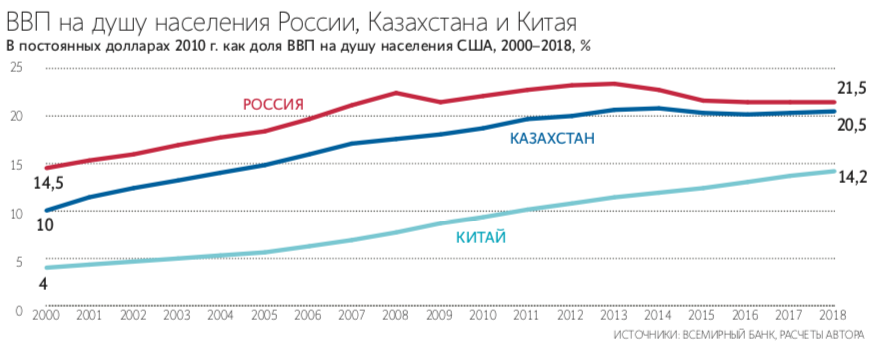
\includegraphics[width=0.68\textwidth]{img/1tbz.png}
    \end{center}
\end{wrapfigure}
\textbf{Авторитарный дедлок.} Более жесткие деспотические режимы политологи называют «авторитарной гегемонией». На выборах здесь авторитарный лидер или правящая партия регулярно получают от 75 до 99\% голосов. Что, однако, свидетельствует не об их популярности, а о том, что они оказывают гораздо более систематическое давление на оппозицию, независимые СМИ и нелояльные элитные группы, т. е. отличаются от предыдущего типа резко возрастающим уровнем репрессивности. Встречаются они сегодня почти исключительно в Азии, Африке и бывшем СССР.

Как показывает опыт ряда азиатских стран, эволюция режима от первого типа ко второму часто происходит на фоне ухудшения экономической динамики. По мере того как экономика играет все меньшую роль в обеспечении легитимности и устойчивости режима, все большую роль начинают играть две другие опоры: репрессии и идеология. В информационной политике режим переходит от фильтрации и ограничения информации к агрессивной пропаганде. Начинаются систематические преследования гражданского активизма, появляются нормы, позволяющие в уголовном порядке преследовать за слова, криминализуется уличная активность граждан.

Именно переход от режима конкурентного авторитаризма к авторитарной гегемонии составил политическое содержание последнего путинского периода – с 2013 по 2019 г. А геополитическая конфронтация выступила в качестве той идеологической рамки, которая легитимирует возрастающую репрессивность.

Хотя Россия выглядит сегодня гораздо более авторитарной страной, чем в 2012 г., этот переход, видимо, следует считать пока незавершенным. Наверное, играют свою роль развитая социальная инфраструктура мегаполисов, уровень европеизированности элит, глубина проникновения интернета и социальных медиа. Ну, и разумеется, экономический застой. Несмотря на это, Путин вряд ли оставит свои усилия по девестернизации России. И это бесплодное (в исторической перспективе) перетягивание каната скорее всего останется главным сюжетом финальной фазы его политической карьеры.





\chapter{Еда и Рецепты}
\section{Как приготовить борщ по классическому рецепту}
\textit{Источник: \url{https://lifehacker.ru/classic-borshcht/}}

В Киевской Руси борщ готовили из съедобных листьев борщевика — отсюда название. Позднее стали варить со свёклой, а с XIX века добавлять картошку.


Сегодня в каждой семье есть свой рецепт борща. В кастрюлю добавляют и фасоль, и грибы, и копчёности, и даже сельдерей. Мы же научим вас готовить идеальный традиционный борщ.

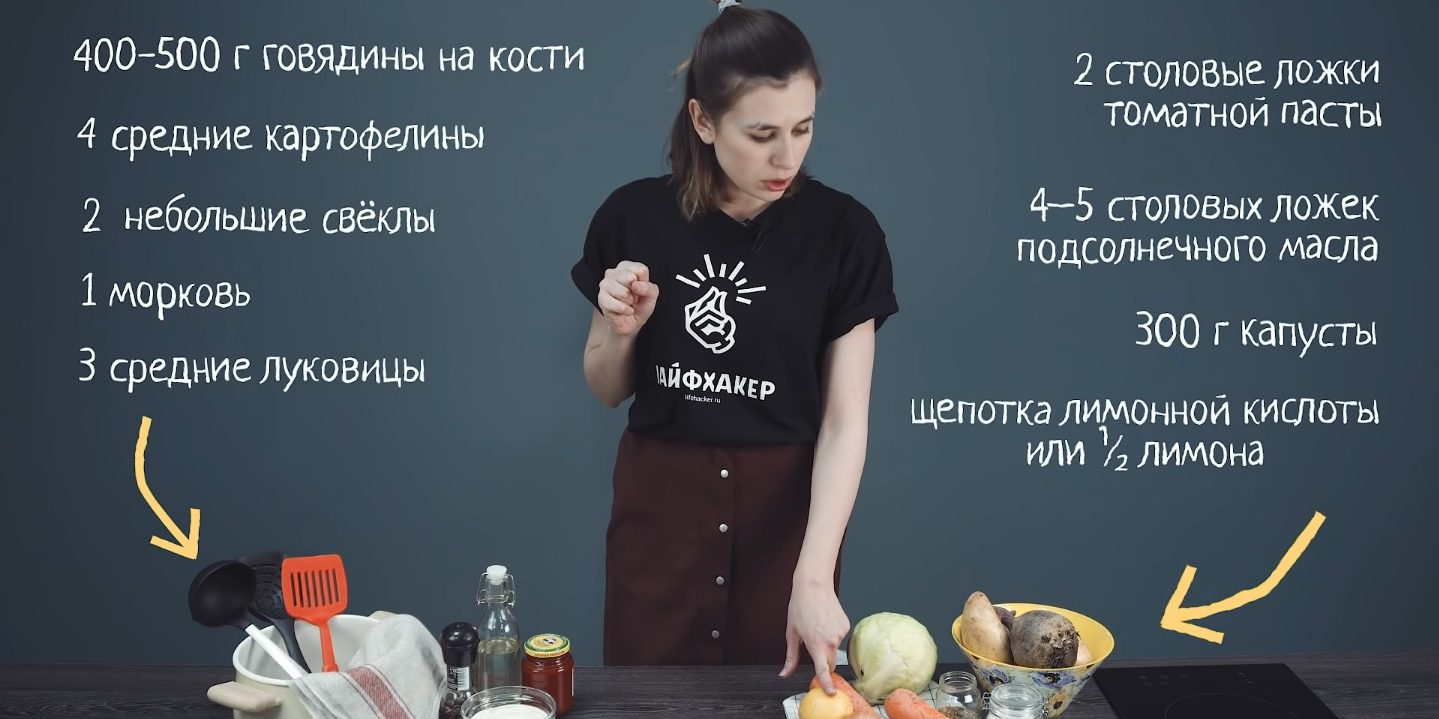
\includegraphics[width=0.75\textwidth]{img/borsch-e1568359200134.jpg}

Для бульона:
\begin{itemize}
    \item 1.5-2 л воды;
    \item400–500 г свинины или говядины на кости.
\end{itemize}


Для зажарки:
\begin{itemize}
    \item 2 небольшие свёклы;
    \item 1 средняя морковь;
    \item 3 средние луковицы;
    \item 4–5 столовых ложек растительного масла;
    \item щепотка лимонной кислоты, немного столового уксуса или ½ лимона;
    \item 2 столовые ложки томатной пасты.
\end{itemize}


Для борща:
\begin{itemize}
    \item 300 г свежей белокочанной капусты;
    \item 4 средние картофелины;
    \item соль — по вкусу;
    \item 1–2 сушёных лавровых листа;
    \item зелень — по вкусу;
    \item 1 зубчик чеснока — опционально;
    \item щепотка молотой гвоздики — опционально;
    \item щепотка молотого чёрного перца — опционально.
\end{itemize}

\textbf{Шаг 1. Сварите бульон.} Налейте в кастрюлю холодную воду, выложите мясо и поставьте на средний огонь. Бульон будет вкуснее, если использовать именно мясо на кости.

Следите за бульоном, перед закипанием снимите пену.

Когда жидкость закипит, накройте кастрюлю крышкой и варите на медленном огне час-полтора.

\textbf{Шаг 2. Сделайте зажарку.}
Вымойте и почистите свёклу, морковь и лук. Свёклу натрите на крупной тёрке, а морковь — на средней. Лук нарежьте небольшими кубиками.

Налейте масло в сковороду, включите средний огонь. Обжаривайте лук и морковь, помешивая, около 5 минут.

Затем выложите свёклу. Добавьте к ней лимонную кислоту, уксус или сок лимона. Благодаря этому борщ будет по-настоящему красным и приобретёт приятную кислинку.

Готовьте зажарку ещё 5 минут. После этого добавьте томатную пасту, перемешайте и оставьте на огне ещё на 5–7 минут.

\textbf{Шаг 3. Соберите борщ.}
Когда бульон сварится, выньте из него мясо. Пока оно остывает, засыпьте в кастрюлю нашинкованную капусту. Через 5–10 минут добавьте нарезанный соломкой или кубиками картофель.

Порядок закладки овощей можно менять. Если капуста молодая, её лучше добавить уже после картошки. Ну или одновременно, если ваш сорт картофеля разваривается быстро.

Пока варится картофель, отделите мясо от кости и нарежьте кубиками. Верните его в суп. Посолите по вкусу.

Добавьте зажарку и перемешайте.

Закиньте лавровый лист и мелко порубленную зелень. Накройте кастрюлю крышкой и варите ещё 5–7 минут.

Для аромата можно добавить в кастрюлю немного измельчённого чеснока, молотой гвоздики или чёрного перца. Оставьте борщ под крышкой настаиваться 5–10 минут.

\textbf{Как подать борщ на стол.} Борщ можно есть сразу после приготовления. Но, как правило, на следующий день он ещё вкуснее.

Добавьте в тарелку сметану и свежую зелень. Если предпочитаете покислее, положите дольку лимона.

Подайте к борщу ржаной хлеб или сдобные булочки, натёртые чесноком. Также блюдо прекрасно дополнят сало и пампушки.
\chapter{Война}

\section{Что ждет россиян во время частичной мобилизации?}
\textit{Источник: \url{https://lenta.ru/articles/2022/09/21/ukaz/}}

\textit{Ответы на главные вопросы}

Президент России Владимир Путин 21 сентября 2022 года объявил о введении в России \ed{частичной}{частичный}{partial} мобилизации. По его словам, призыву на военную службу подлежат граждане, состоящие в запасе, и прежде всего те, кто служил в армии. Кто теперь подлежит призыву, кто имеет право на \ed{отсрочку}{отсрочка}{delay; postponement}, каков порядок мобилизации — в этих вопросах разбиралась «Лента.ру».

\ed{Указ}{ук\'{а}з}{decree} «Об объявлении частичной мобилизации в Российской Федерации» опубликован на сайте Кремля в среду, в 9 часов 20 минут.

«Объявить с 21 сентября 2022 года в Российской Федерации частичную мобилизацию», — сообщается в первом пункте документа, подписанного президентом России Владимиром Путиным.

Во втором пункте указано, что мобилизованные граждане получат статус военнослужащих-контрактников с денежным содержанием соответствующего размера. Увольнение из рядов мобилизованных предусмотрено только по возрасту и по состоянию здоровья.

Правительству поручено финансировать мероприятия по проведению частичной мобилизации, главам регионов — обеспечить призыв находящихся в запасе граждан.

\textbf{Сколько человек призовут?}

Согласно заявлению главы Минобороны Сергея Шойгу — 300 тысяч. Это примерно 1,1 процента от общего мобилизационного ресурса России, который, по словам министра, составляет почти 25 миллионов человек. Для каждого региона количество подлежащих мобилизации будет определяться отдельно.

\textbf{Кого призовут в первую очередь?}

По словам Шойгу, на военную службу по мобилизации будут призваны те, кто отслужил в армии, имеет военно-учётную специальность и соответствующий опыт. Перед отправкой в части они пройдут обязательную дополнительную подготовку.

\ed{Полковник}{полковник}{colonel (army)} \explain{в отставке}{retired} Виктор Баранец считает, что первыми под мобилизацию попадут резервисты, которые каждый год по указу президента призывались на военные сборы, стреляли, водили танки и наводили ракеты. Кроме того, будут призваны люди, по разным причинам уволенные с контрактной службы, а также молодые офицеры.

«Резервисты -- это \explain{военнообязанные}{conscripts; liable for military service} граждане государства, которые подлежат мобилизации при необходимости, -- рассказал в свою очередь «Ленте.ру» \explain{судь\'{я}}{judge} в отставке Владимир Комсолев. —- В нашем случае это лица, прошедшие службу и имеющие достаточную подготовку. Они заключили контракт о пребывании в резерве и получают за это деньги. Раз в год резервисты выезжают на военные сборы, раз в месяц участвуют в занятиях».

Юрист Артем Мугунянц в разговоре с «Лентой.ру» отметил, что тех, кто пользовался отсрочкой в период с 18 до 27 лет и не служил, мобилизация, вероятно, не коснётся.

«Мобилизации подлежат только те, кто служил в армии либо офицером, либо проходил срочную службу, либо был контрактником\footnote{Only those who served in the army either as an officer, or did military service, or were a contract soldier \textit{are subject to} mobilization}. — пояснил эксперт. — Можно предполагать следующее. Так как утверждается, что необходимо освобождать территории Украины, им потребуются \explain{наступательные войска}{offensive troops}: танкисты, \explain{морская пехота}{marines}, мотострелковые части. Эти части и войска могут потребоваться в большом количестве. Тех, кто служил в этих войсках, будут мобилизовать в первую очередь».

\textbf{Людей какого возраста могут призывать?}

Согласно статье 53 Федерального закона «О воинской обязанности и военной службе», все военнослужащие запаса делятся на три разряда. В случае мобилизации первым в ВС попадает первый разряд, затем — второй, третий — последним (подробнее о том, что значат категории запаса и категории здоровья — ниже).

По первому разряду призываются солдаты и низшие \ed{чины}{чин}{rank} в возрасте до 35 лет, младшие офицеры в возрасте до 50 лет (в третьем разряде верхние рамки для этих званий повышаются до 50 и 60 лет соответственно) и так далее. Представители генералитета подлежат мобилизации по второму разряду в возрасте до 70 лет.

В Госдуме заявили, что планируют призывать тех, кто попадает под первый разряд.

«Пока человек не снят с военного учёта, он может подлежать мобилизации, — пояснил «Ленте.ру» профессор кафедры уголовного права РГПУ имени А.И. Герцена Сергей Милюков. — Есть специальности в ближнем и дальнем тылу, где возраст не является большой \ed{пом\'{е}хой}{пом\'{е}ха}{hindrance}. Например, обязательно потребуются медики. Призванные врачи будут оказывать медпомощь в госпиталях в тылу. Для лечения и \ed{дол\'{е}чивания}{дол\'{е}чивание}{follow-up treatment} нужно привлечь санатории, как это было в Великую Отечественную войну. Непосредственно же в боестолкновениях должны участвовать более молодые люди».

\textbf{Что означают категории запаса и категории здоровья в военном билете? }

Существует пять категорий годности к военной службе. Их определяют исходя из показателей здоровья и записывают данные об этом в военном билете.
\begin{itemize}
    \item «А» — \explain{годен}{fit} к военной службе;
    \item «Б» — годен к службе с \ed{незначительными}{незначительный}{insignificant} ограничениями;
    \item «В» — ограниченно годен к военной службе;
    \item «Г» — временно не годен;
    \item «Д» — не годен к несению военной службы.
\end{itemize}
Группы здоровья «А», «Б» и «В» по федеральному закону \explain{подлежат}{are subject to} мобилизации.

Всех резервистов \ed{распределяют}{распределять}{distribute} по трем категориям в зависимости от возраста военнослужащего и полученного звания.

Первая категория — граждане, которых призывают в первую очередь в случае мобилизации. \explain{Речь идет о}{This is a very useful expression; it means ``this is about...''} военных, которые не получили офицерский чин (в том числе \ed{прапорщики}{прапорщик}{ensign} и мичманы) и не \explain{перешагнули}{stepped over} возрастной \explain{пор\'{о}г}{threshold} в 35 лет, а также о младшем офицерском составе до 45 лет (лейтенант, капитан). В данной категории числятся старшие офицеры до 50 лет (майор, \explain{подполковник}{lieutenant colonel}); полковники, капитаны 1 ранга до 55 лет; высшее руководство до 60 лет. Первым на службу должен прибыть офицерский состав высшего эшелона.

Вторая категория — военнообязанные старшей возрастной группы или те, кто не прошел в первую волну мобилизации по здоровью. В эту группу попадают солдаты, военнослужащие без офицерского звания в возрасте от 35 до 45 лет, младший руководящий состав от 45 до 50 лет и старшие офицеры от 50 до 55 лет.

Третья категория — военнослужащие, которых призывают только в том случае, если военные действия длятся больше года и необходимы дополнительные силы. Под эту категорию попадают \explain{рядовые}{privates} и \explain{матросы}{sailors}, прапорщики и мичманы самой старшей возрастной категории. Возраст низшего\footnote{низкий, низшего} офицерского состава этой категории до 55 лет, а для капитанов 2 и 3 ранга и подполковников — до 60 лет. В данной категории пребывают военнообязанные женщины в возрасте до 50 лет.

\textbf{Что такое мобилизационное предписание? }

Это документ, который выдается части запасников. Выдача мобилизационного предписания — это \explain{своеобразная}{peculiar, singular, sui generis} перепись военнообязанных лиц. Гражданин, который получил мобилизационное предписание, при объявлении мобилизации должен прибыть в указанное в нем место и срок без дополнительной \ed{повестки}{повестка}{subpoena, writ} и предупреждения.

Как \explain{утверждает}{claims} юрист Павел Чиков, во время мобилизации гражданам приходят повестки, как и в обычное время — лично в руки или под подпись. Повестку также могут вручить по месту работы.

Однако именно запасники, имеющие мобилизационные предписания, по статье 21 ФЗ «О мобилизационной подготовке и мобилизации в Российской Федерации» самостоятельно должны \explain{явиться}{show up} в военный комиссариат.

\textbf{Кто имеет право на отсрочку?}

Как следует из указа, подписанного Путиным, \ed{отсрочку}{отсрочка}{postponement} пол\'{у}чат работники оборонных предприятий. «\explain{Предоставить}{provide} гражданам Российской Федерации, работающим в организациях оборонно-промышленного комплекса, право на отсрочку от призыва на военную службу по мобилизации (на период работы в этих организациях). Категории граждан Российской Федерации, которым предоставляется право на отсрочку, и порядок его предоставления определяются правительством Российской Федерации», — говорится в документе.

Как следует из статьи 18 федерального закона о мобилизации, отсрочка также предоставляется:

\begin{itemize}
    \item временно \ed{негодным}{негодный}{ineligible, not qualified} к военной службе по состоянию здоровья;

    \item ухаживающим за близкими родственниками, которых больше некому содержать;

    \item многодетным родителям (тех, кто имеет на \ed{иждивении}{иждив\'{е}ние}{dependent} не менее четырех детей в возрасте до 16 лет или троих детей при условии беременности супруги сроком не менее 22 недель);

    \item родителям-одиночкам;

    \item членам Совета Федерации и депутатам Госдумы.
\end{itemize}

Другие категории военнообязанных, которым \explain{полагается}{depends, relies} отсрочка (бронь от призыва), еще не известны. Их определяет правительство России, напомнил пресс-секретарь президента Дмитрий Песков.

\textbf{Попадают ли под мобилизацию срочники и те, кто не служил в армии? }

По закону о мобилизации — не попадают. Из него следует, что в ряды вооруженных сил должны быть направлены «граждане, пребывающие в запасе, не имеющие права на отсрочку от призыва на военную службу по мобилизации».

По словам юриста Ольги Лютницкой, \explain{срочники}{conscript} не попадают под эту категорию, так как они еще не переведены в запас.

Если гражданин не служил, например, потому, что был ограниченно годен, но у него есть военный билет, то веротность его мобилизации есть, сказала она «Ленте.ру».

Юрист Мугунянц уточнил, что срочники уже являются военнослужащими по призыву. Задействовать их до объявления полной мобилизации и войны нельзя.

\textbf{Можно ли мужчинам теперь выезжать за границу? }

В Федеральном законе «О мобилизационной подготовке и мобилизации в Российской Федерации» говорится, что «гражданам, состоящим на воинском учете, с момента объявления мобилизации воспрещается выезд с места жительства без разрешения военных комиссариатов, федеральных органов исполнительной власти, имеющих запас».

Юрист Лютницкая утверждает, что пока по вопросу \ed{запрета}{запрет}{ban, prohibition} выезда мужчинам за границу нет никаких законодательных актов и комментариев. Поэтому прямо сейчас никаких ограничений для выезда не существует.

Юрист Мугунянц также отметил, что выезжать никому не запрещено: выезд закрывается только при полной мобилизации.

«Если же человека мобилизовали, то есть признали военнослужащим, дали мобилизационное предписание о том, что он должен явиться, то он действительно не может выехать в другую страну. Потому что он мобилизован», — уточнил эксперт.

При этом скорее всего человека не будут вносить в каике-либо базы, но гражданин должен \explain{учитывать}{take into consideration}, что выезд будет расценен как \explain{уклонение}{evasion} от армии, за которое возникнут соответствующие \explain{уголовные последствия}{criminal implications}.

Член Совета по правам человека при президенте России Кирилл Кабанов заявил, что для людей без повесток на руках юридического запрета на выезд за границу нет.

\textbf{Что ждет тех, кто по достижении 27 лет получил справку вместо военного билета?}

Те, кто не проходил службу в вооруженных силах \explain{без уважительной причины}{without good reason} (например, сознательно \ed{уклонялся}{avoided, dodged}), и по достижении 27-летнего возраста получил справку \explain{взамен}{instead of} военного билета, вероятно, не будут призваны во время частичной мобилизации, так как они тоже — не служившие люди, считает юрист Мугунянц.

«На данном этапе у них никаких проблем нет. Если объявят всеобщую мобилизацию, то [обладателей справок] будут призывать, как и всех. К ним будут применяться те же условия, как к людям, которые не служили, но имеют военный билет. То же касается и тех, кто вообще не имеет никаких документов [подобного рода]. Важно, что они находятся в мобилизационном возрасте и подпадают под [всеобщую] мобилизацию».

По российскому законодательству, обладатель справки не может быть принят на государственную службу, в остальном его права не отличаются от прав владельца военного билета.

\textbf{\explain{Затрагивает}{affects} ли мобилизация женщин?}

По закону, мобилизация граждан, пребывающих в запасе, \explain{предполагает}{suggest} возможность призыва на военную службу медработников женского пола в возрасте до 45 лет. У них на руках есть военные билеты — медработники получают их после учебы.

Адвокат Владимир Шелупахин объяснил «Ленте.ру», что призыв состоящих на воинском учете женщин предполагается только в третью очередь, то есть после мужчин в возрасте 35-45 лет, в том числе граждан, пребывающих в запасе, но годных к военной службе с незначительными ограничениями (категория «Б») или ограниченно годных к военной службе (категория «В»).

«\ed{Вовсе}{вовсе}{at all} \explain{освобождаются}{released} от службы матери-одиночки и многодетные матери», — добавил юрист. Кроме того, на женщин распространяются и другие отсрочки, описанные в федеральном законе.

\textbf{Могут ли повестки приходить через «Госуслуги»?}

По официальной информации — нет. О возможной отправке повесток через сервис \ed{Госуслуг}{Госуслуги}{public services} 21 сентября написал Telegram-канала Baza. По информации издания, всем, кого собираются призвать, придет уведомление в аккаунте Госуслуг дополнением к обычным повесткам через почту.

Однако в Минцифры почти сразу это \explain{опровергли}{refuted}. «В связи с появившимися в соцсетях публикациями о том, что электронные повестки в рамках частичной мобилизации будут \explain{рассылаться}{be sent out} через Госуслуги, сообщаем, что таких планов нет. Необходимая законодательная база для этого отсутствует», — говорится в Telegram-канале министерства.


\section{Таких замученных людей я раньше не видел}

\textit{Рассказ россиянина, который несколько суток пытался уехать в Казахстан }

\textit{Источник: \url{https://baza.io/posts/4250c126-5344-458d-af97-21179596c136}}

Сутки на жаре и холоде, драки, голод и бессонница. Со всем этим столкнулся Александр, который после объявления о «частичной мобилизации» решил уехать на машине в Казахстан. Однако там его, как и тысячи других россиян, встретил своеобразный тест на выживание и целый ряд гуманитарных проблем.

Это детальный рассказ Александра о том, что сейчас происходит на границе с Казахстаном в Астраханской области.


\textbf{Добраться до границы}

Мчались к границе под Астраханью в режиме аврала: за ночь собрали чемоданы, бросили ключи от квартиры с котом друзьям и полетели в Волгоград, так как только туда в эти дни были нормальные цены на билеты. Самолёт был полностью забит мужчинами. Когда заходил, услышал, как одна бортпроводница шепнула другой насчёт пассажирки: «О, девушка, ничего себе! Впервые за два дня».

Уже в самолёте стало ясно: ехать, как мы планировали, на поезде до Астрахани очень долго, и потому прямо в аэропорту взяли таксиста. Спросили, за сколько он довезёт до границы под Астраханью, и он, назвав сумму в 15000, сразу получил её в руки. Мы гнали больше ста весь путь. В какой-то момент водитель даже чересчур заспешил и чуть не размазал нас по встречной фуре.

Остановились только один раз — на пустынной заправке у трассы. Там был заправщик, который принялся нам угрожать и затевать драку из-за того, что мы бежим из страны. Мы ничего ему не говорили, но ему было очевидно, что мы москвичи, так как он обронил «из-за таких, как вы, у меня всех братьев забрали».

Обидно было, что он именно нас в этом обвиняет, а не власть. Но вместе с тем жалко парня: многим очевидно, что в сёлах больше пропорции набора.


\textbf{Звёзды и безысходность под Астраханью}

Подобрались к границе Астрахань — Атырау с наступлением темноты, тогда длина пробки до КПП была уже 14,9 километра. Там уже царила анархия: нам с ходу предложили купить велосипед за 50000 рублей, на котором можно было проехать границу. Далее следовал жуткий марш-бросок в кромешной тьме с чемоданами под дождём в дикий холод: вместе с тьмой на пробку опустилась осенняя прохлада и ливень.

Мы прошли вместе с чемоданами около 8 километров, разглядывая, как люди друг с другом ругаются из-за мест, как плачут уставшие дети в машинах, как кричат кошки в переносках. Люди пытались лечь спать в совершенном аду. Над нами, стоит отметить, висело фантастически красивое звёздное небо: в радиусе километров не было огней, и это был фантастический вид на звёзды. Но вместе с тем впервые пришло отчаяние: стало понятно, что выжить тут будет нереально.

Вокруг сновали люди на велосипедах с подвязанными к спине чемоданами, люди на гироскутерах, самокатах, местная банда бородатых наглецов, отжимавших места поближе к границе на продажу, и огромная, невообразимая по длине пробка из легковых и большегрузных машин, у которой не было конца. Спустя два часа такого движения, не найдя конца очереди, мы устали смертельно, и пришло понимание: либо мы сейчас едем в аэропорт и домой, либо должны немедленно устроиться на ночлег. Я был замерзший, мокрый и абсолютно раздавленный безысходностью.

И тут я увидел паренька лет 20, который ехал один в этой пробке на своей машине. Ходили слухи, что пробку на машине можно преодолеть только за сутки-полтора, и я удивился: как он в одиночку, без смены собирался ехать такой период времени без остановки? Мы предложили ему за деньги взять нас до границы, пообещав подменять за рулём для сна. Парень согласился, и мы залезли в машину. Боже, как было уютно и тепло после холодной дождливой улицы! Мы часа три-четыре ехали с ним, стараясь лавировать между дальнобойными машинами, которые пытались блокировать дорогу бомбилам, занимающим места. При этом мы весело болтали за жизнь. Стало понятно, что компания приятная.

Я чувствовал, что дико устал. Время уже было около часа ночи, как вдруг движение встало. Перед нами была вереница дальнобойщиков, уходящая в бесконечную даль, и мы в ожидании, когда вновь начнётся движение, заглушили двигатель и в какой-то момент уснули.


\textbf{«Голодные игры»}

Я проснулся спустя пару часов: было холодно даже внутри машины, хотя спал я в куртке. Парень, который нас взял, курил возле авто, закутанный во всю одежду, что у него была. Мы стояли окружённые со всех сторон дальнобойщиками, которые спали в кабинах. А вокруг был шум двигателей. Казалось, все едут, и только мы стоим в своём маленьком дальнобойном ряду.

Парень сходил на разведку и вернулся с криком «Погнали!». На часах было только 4 утра, и тьма была непроглядная. Мы очень аккуратно вылезали между дальнобойщиками на обочину и, когда выехали, увидели сцену из какого-то плохого спин-оффа фильма «Голодные игры»: сотни автомобилей носятся по полю, пытаясь обогнать друг друга в пробке на дороге и влезть где-то ближе к первому блокпосту ГИБДД.

Мы вместе со всеми выехали на поле и оказались в абсолютной мясорубке: ночь, вой моторов и сотни водителей, выдавливающих друг друга с дороги в кювет. Уже не знаю, как у паренька это вышло, но благодаря своей наглости и терпению он нашёл небольшой перекрёсток с просёлочной дорогой, чтобы вклиниться, и мы заняли позицию до рассвета.


Рассвело к шести, и на перекрёстке появился сотрудник ГИБДД. Он пытался разрулить весь тот кошмар, который произошёл за предрассветные часы. Водителей, ждущих в пробке уже сутки, это злило: кто-то за ночь влез без очереди из-за дальнобойщиков, которые заблокировали поток в знак отместки за потерянное время. Теперь такие водители не давали сотруднику ГИБДД пропускать влезшие с обочины машины.

Инспектор был абсолютно уставший и измождённый и в какой-то момент просто ушёл, оставив всё это дело жить своей жизнью. А жизнь была такая: пока на горке совершали намаз мусульмане, семьи с детьми пытались умыть уставших и невыспавшихся детей, а кто-то гулял с собакой, привезённой с собой в этот кошмар.

«Нам тут не влезть», — хмуро сказал наш водитель, и мы пошли искать сообщников на прорыв. Картина открывалась жуткая. Поговорив с окружающими, мы узнали, что люди, стоявшие в честной пробке, провели здесь уже сутки, тогда как наш маршрут занимал около 10 часов. Многие были с детьми, пожилыми родителями, животными. Кто-то из них набрал попутчиков. Но всех объединяло одно: все они, так же как и мы, ночью были заблокированы колонной дальнобойщиков.

Услышав шум машин и оскорбившись такой наглостью, водители бросились объезжать их по полям, перемешивая все очередности. Этот перекрёсток был всего в 5 километрах от границы.


\textbf{Банка майонеза, драки и ФСБ}

В пробке было много машин с Северного Кавказа: с номерами из Дагестана, Чечни, Ингушетии. Они везли семьи, детей, родителей: их семьям угрожало наказание за то, что они уклоняются от мобилизации, потому всех брали с собой. Здесь же были и напуганные студенты, и взрослые мужчины, и ребята со всей страны: Ростовской, Краснодарской областей, попадался Санкт-Петербург и Карелия. Представьте, люди приехали сюда из Карелии!

Куда, спрашиваю у водителя, здесь ходят в туалет? Он смеется: «А как ты думаешь? Спустись с дороги». И тут я увидел страшное зрелище: отходить от дороги далеко нельзя — вдруг твоё место займут? Тех, кто ушёл дальше 50 метров, разворачивали пограничники. Поэтому люди были вынуждены ходить в туалет прямо здесь, на глазах всей пробки. Десятки тысяч людей, женщин, мужчин, любых вероисповеданий и культур. Все делали это здесь.

Обстановка накалялась: люди не могли поделить дорогу, и вспыхивали драки в разных частях пробки. Солнце окончательно поднялось, и стало жарко. Ещё ночью ты заворачивался во все вещи из чемодана, а сейчас потел в футболке.

Стало понятно, куда уехал сотрудник ГИБДД: он вернулся с группой пограничников и бойцами ФСБ на «Барсе». Они подняли оружие, будто угрожая начать пальбу в воздух, но толпу это мало пугало: несколько ретивых ребят попытались втянуть в драку инспектора. Только с появлением майора ГИБДД — уставшего, с выгоревшей на солнце кожей и грозным голосом — удалось сбить накал и договориться о системе проезда. Разумеется, и она не соблюдалась. Как только инспектор принимался разруливать проблему в одной точке пробки, вспыхивали бои в другой.

Мы смогли въехать на точку, указываемую в многотысячных чатах пробки как ключевую, после которой «ад заканчивается» и «всё становится интеллигентно». Здесь находился узкий мост, и далее авто двигались в образовавшейся колонне одна за другой. Ну как двигались: за 12 часов все продвинулись на 600–700 метров, не более.

Тут появилась гуманитарная проблема: у кого-то заканчивалось топливо, у кого-то еда и вода для детей и взрослых. Некоторые были отправлены в город за едой, но тут же попадали в капкан: их машины не хотели пропускать обратно в задней части пробки, и эти машины выбывали из общей гонки.

К этому времени о пробке уже трубили СМИ. Новости от тех, кто был на границе, расстраивали: они стояли по трое суток. Мы достигли посёлка, в конце которого находился КПП, только к темноте. В посёлке в это время совершенно опустел магазин: только одинокая банка майонеза стояла в пустом холодильнике. Проблема с водой, едой и топливом решена не была: люди в моей части колонны делились этим с соседями, некоторые продолжали толкать машину, чтобы не заводить авто и не тратить топливо. Я отдал две из трёх оставшихся бутылок воды в соседние машины с детьми, а также раздал большую часть своей аптечки. Особенно было популярно обезболивающее.


Обочина в этой части была полна мусора от наших предшественников, а также сбежавшимися на него собаками. Это отпугивало людей от туалета. Еда почти у всех кончилась, наступила ночь, и снова стало холодать.

На помощь пришли жители посёлка. Они за крайне низкие цены стали продавать еду, заряжать телефоны, бесплатно пускать в туалет, а детей — отдохнуть в дома. Но вместе с темнотой пришла и новая проблема: организованные «мафиози» держателей мест вклинивались в ряды. Их целью было удержать позицию в этой части пробки и продать их тем, кто прибыл в конец.

По слухам, место в этой части пробки стоило по 25–30 тысяч рублей. Это приводило к конфликтам и дракам, маханию ножами и угрозам убийством. На самые громкие драки прилетали сотрудники ФСБ на «Барсе», в балаклавах и с автоматами. Это успокаивало конфликтующих — до отъезда офицеров.


\textbf{Дорожная «мафия»}

Здесь, в 4 километрах от границы, уже было много пешеходов с сумками. Они доходили до этой части колонны и просились в машины: переходить границу пешком было нельзя. У обочины были свалены велосипеды: люди, накупившие их в конце пробки за 30–50 тысяч рублей, у КПП узнавали, что на велосипеде было всё-таки нельзя. Пеших кто-то подсаживал бесплатно, а кто-то брал за деньги. И тут начался новый коллапс: каждый, кто слышал о более высокой цене, поднимал цену у себя, и в итоге стоимость места в машине выросла до 40–50 тысяч рублей.

Чем темнее становилось, тем активнее начинались бои во второй части «Голодных игр». Вместе с этим накопилась усталость: за двое суток, из которых на сон пришлось 3 часа, мы не выспались. Первоначальный план, согласно которому мы хотели меняться местами с водителем, разбился о необходимость вылетать из машин по свисту — для обороны мест от влезавших барыг-продавцов. Это длилось всю ночь.

Третьи сутки прошли по абсолютно такому же сценарию, но изменились цены: мы были уже в 2 километрах от КПП, и цены на места для пассажиров достигали 70 тысяч. Еда и вода стали дефицитными, мы совсем отказались от еды в пользу детей, водой нас снабжали местные жители совершенно бесплатно. Для экономии топлива многие стали толкать машины. Чтобы хоть как-то спать, часть не умеющих водить пассажиров освоили основы вождения.

К ночи началась третья серия «Голодных игр» с ещё более активным противостоянием. Здесь уже оставалось менее 500 метров до КПП, и дорога была блокирована десятками мужчин, утверждавших, что это их территория, а машины будут пропускаться по системе «шесть из колонны — одна их».


«Одна их» представляла собой минивэн с вместимостью 6–12 человек, куда сажали пешеходов по цене от 70 до 90 тысяч рублей за место. На дороге появились «служебные машины» с сопровождением ГИБДД, следовавшие в сторону КПП. В числе служащих были замечены пожилые женщины и подростки. Обратно они не возвращались.

Бои длились до утра. Под эффектный рассвет мы пересекли КПП. Там все уже были знакомы: сотрудники ФСБ, помогавшие отвоёвывать места, пограничники, с уставшими лицами проезжавшие мимо пробки на микроавтобусе, работники ГИБДД, нервно курившие после изнуряющей смены в ночном кошмаре.

На КПП были и молодые люди, которых задержали в связи с тем, что они получили повестки. Стало ясно, что слухи о списках на границах вовсе не были слухами.


\textbf{Переход}

Под встающее солнце мы с уже родными соседями пересекали границу и неслись по буферной зоне, в которой, как нам завещали сотрудники российской погранзаставы, не стоит покидать автомобиль. Проехав шесть километров из двенадцати, мы уткнулись в новую пробку.

У буферной зоны была особенность: здесь не было ни сотрудников ГИБДД, ни ФСБ. Зато были свои барыги: они перевозили людей за 30–50 тысяч от одного КПП до другого через встречную полосу. Здесь они были более подготовлены и ездили по двое, с охраной. Но и люди, попавшие в эту зону, были уже ветеранами и прямо между двумя погранзаставами мастерили себе примитивное оружие близкого боя. Как ни странно, боёв не было. Но день прошёл в столкновениях и наездах машин барыг на активистов пробки.

Моторы здесь не заводились, даже для движения в горку, пить воду перестали даже женщины, кто-то набирал воду из местной реки, которая оказалась достаточно чистой. Не было слёз и истерик: к четвёртым суткам погранперехода плакать уже не умели, лишь сурово грустить. Я был знаком с людьми на десятки машин назад и вперёд: отличные ребята со всей европейской части страны, бегущие от правительства и безысходности.

Организовывались сигналы тревоги и группы быстрого реагирования для непропуска барыг. Дальнобойщики, чудом прорвавшиеся в эту зону, грели воду для бытовых нужд: некоторые впервые за эти дни чистили зубы или умывались. На реке появилась лодка: в ней приплыла семья из республики Северного Кавказа, пересекшая таким образом границу: они бесплатно раздавали всем еду, воду и лекарства.

К ночи приехали российские пограничники. Они строго запретили покидать автомобили: таковы были правила проезда. Исключения сделаны были для тех, кто толкает машины. К глубокой темноте мы прошли мост — переход через границу и встали в очередь к казахскому КПП.

Последний этап этого квеста был связан с полным отсутствием сил. Без еды, сна и покоя мы провели по четверо суток. Впереди было ещё шесть часов в пробке. Появился интернет, а вместе с ним в чате пробки появилась информация о местах в машине по 150000 рублей и барыгах, которые перевозили людей в нейтральную буферную зону за одну сумму, а уже в буферной зоне требовали другую. Те, кто не соглашался, отправлялись обратно.

Водители засыпали за рулём: сказывались по 80–96 часов без отдыха. Все были измождены и глубоко несчастны. Казахские пограничники встречали людей сочувствием и крайне лояльным досмотром. Впервые показалось, что мы действительно беженцы: таких несчастных и замученных людей я раньше не видел.

Впереди у нас было ещё шесть часов по бездорожью в степи до ближайшего города.



\chapter{Личность, Характер и Психология}
\section{Что такое думскроллинг}

\textit{и почему чтение плохих новостей пагубно влияет на ментальное здоровье?}

\textit{Источник: \url{https://www.elle.ru}}
% https://www.elle.ru/otnosheniya/psikho/chto-takoe-dumskrolling-i-pochemu-chtenie-plokhikh-novostei-pagubno-vliyaet-na-mentalnoe-zdorove/

\begin{fancyquotes}
    Постоянно просматриваете новости? Не выпускаете смартфон из рук? У нас для вас плохие новости  ---  вы зависимы, и это пагубно влияет на ваше здоровье и умственные способности.
\end{fancyquotes}

Думскроллинг (от английского doom  ---  «гибель, судьба, рок, Судный день» и scrolling  ---  «прокрутка»)  ---  это склонность к просмотру и чтению плохих новостей, несмотря на то, что они вызывают негативные эмоции, удручают, огорчают и деморализуют. Термин стал относительно широко использоваться в начале пандемии и сейчас снова стал актуален на фоне нестабильной ситуации в мире. Так почему же мы не можем оторваться от плохих новостей и как это влияет на наше психоэмоциональное состояние?

Основная причина бесконтрольного думскроллинга  ---  это боязнь пропустить важные новости. Беспокойный ум стремится понять, что происходит в мире и как это может коснуться лично нас. В таком случае думскроллинг дает ощущение контроля над ситуацией. Интуитивно мы пытаемся подготовиться к потенциальным угрозам. Принцип «предупрежден  ---  значит вооружён» миллионы лет способствует выживанию людей как вида.

\textbf{Почему это вредно?}

Иллюзия контроля над ситуацией, по большому счету, не дает никаких преимуществ. Думскроллинг способствует развитию тревожности и стресса, повышается вероятность панических атак, снижается концентрация. Умные алгоритмы соцсетей предлагают все больше и больше плохих новостей, поиск и чтение пугающих статей превращается в зависимость, человек игнорирует собственные мысли и чувства. Впоследствии чтение негативных новостей может приводить и к ухудшению сна и истощению нервной системы.

\textbf{Как бороться с думскроллингом?}

Не пользуйтесь гаджетами перед сном. Не читайте новостей о коронавирусе, войнах, протестах и других тревожных явлениях на ночь. Если вам сложно контролировать это самостоятельно, то установите будильник и за 2-3 часа до сна переводите телефон в авиарежим.

Читайте только ту информацию, которая вам нужна, не переключайте внимание на другие новости. Перед тем, как читать новости и статьи в интернете, четко определите «цель визита», не обращайте внимание на предложенные статьи или кликбейтные заголовки.

Отвлекитесь от новостного контента. Попробуйте сместить фокус внимания с новостей на интересные статьи, интервью, рецензии.

Займитесь чем-то другим. Кино, музыка, встречи с друзьями  ---  все это поможет провести вам время с куда большей пользой для нервной системы.

\newpage
\section{Синдром спасителя}

\textit{Как добрые намерения скрывают эмоциональные недостатки}

\textit{Что скрывает навязчивое желание помочь ближнему, если вас об этом никто не просит}

\textit{Источник: \url{https://www.elle.ru}}
% https://www.elle.ru/otnosheniya/psikho/sindrom-spasitelya-kak-dobrye-namereniya-skryvayut-emocionalnye-nedostatki/

Проявления синдрома спасителя не всегда очевидны для окружающих и даже тех, кого непрошеные благодетели окружают заботой. Импровизированные супергерои всегда готовы помочь нерасторопным коллегам, спасти близких (и не очень) людей от жизненных невзгод и пагубных пристрастий. Именно такие светлые человечки рады круглосуточно наставлять подшефных по вопросам правильного питания, карьерного роста и токсичных отношений. Ведомые убеждением, что в этом их высшее предназначение, «спасители» возводят альтруизм в культ, в действительности скрывая за самоотдачей эгоизм и невротические изъяны.

Термин «спаситель» используется психологами с 1968 года, с тех пор, как доктор Стивен Карпман, ученик Эрика Берна и знаток транзактного анализа, раскрыл в опубликованной работе модель социального и психологического взаимодействия, названную в его честь «треугольник Карпмана» (он же  ---  «треугольник судьбы» или Karpman drama triangle). В статье Fairy Tales and Script Drama Analysis американский ученый описал три привычные роли, которые мы часто играем в разных ситуациях: жертва, преследователь и спаситель, который вмешивается, как кажется, из желания помочь тому, кого обижают или недооценивают.

Как разъяснил Карпман, ролевая игра, схожая с мелодраматическим сюжетом про «героя, злодея и девицу в беде», раскрывает неочевидный мотив: спаситель заинтересован поддерживать жертву в ее зависимости от себя. Догадываетесь почему?

\textbf{Как из заботы получается созависимость}

«Нужда помогать другим движет личностью, способной реализоваться исключительно в опеке других,  ---  объясняет Анн-Виктуар Русселе, парижский психолог и терапевт.  ---  Такие люди считают своим долгом спасать других в ущерб себе, включая тех, кто в этом абсолютно не нуждается. Они сознательно вступают в созависимые отношения, считая, что не заслуживают любви партнера, но убеждая себя, что эта связь оправдана желанием избавить ее/его от проблем. Настойчивая услужливость имеет в корне нарциссический изъян, скрывающий неуверенность в себе и сопутствующую мотивацию: потребность поднять самооценку. „Спаситель“ становится лучше в собственных глазах, проецируя на ближних позитивные намерения и поступки».

Чего же следует ожидать от непрошеной заботы? «Спасаемые» увиливают от спасения, не предлагая взамен долгожданной компенсации, что, естественно, отзывается в душе супергероя горьким разочарованием. «Я делаю все для всех, но никто никогда ничего не делает для меня»,  ---  типичная жалоба отвергнутого спасителя.

«Последствия амбивалентного синдрома непременно дадут о себе знать,  ---  пишут калифорнийские психологи Мэри Ламиа и Мэрилин Кригер в книге „Синдром Белого Рыцаря: спасение себя от потребности спасти других“ (The White Knight Syndrome: Rescuing Yourself from Your Need to Rescue Other).  ---  В начале отношений спаситель кажется удовлетворенным своей самоотверженностью, но со временем становится все более несчастным и бессильным. Она/он буквально выдыхается, теряя смысл, интерес, энергию, ресурсы, что, в свою очередь, отражается на самооценке. Убедившись, что усилия напрасны, «белый рыцарь» выходит из игры эмоционально и психологически истощенным».

\textbf{В чем (опять) виноваты детские травмы}

Потребность спасать указывает на эмоциональный и психологический дисбаланс, ноги которого предсказуемо растут из воспитания, образования и внушенных ценностей. «Она/он спасает всех вокруг, стараясь быть „хорошей девочкой/мальчиком“, чтобы получить одобрение со стороны реального или внутреннего родителя и укрепить самооценку,  ---  описывает природу травмы доктор Русселе.  ---  Возможно, в детстве „спасителю“ приходилось помогать больной матери, заботиться о братьях и сестрах, с раннего возраста посвящая себя нуждам взрослых и опуская свои потребности в нижний ранг приоритетов».

Пресловутый дисбаланс имеет тенденцию преследовать «спасителя» до зрелости, поддерживая в ней/нем потребность окружить себя партнерами, друзьями и коллегами, о которых нужно будет заботиться. И эта иллюзорная стратегия предсказуемо обречена на неудачу, потому что суть всего успешного базируется на гармонии.

\textbf{Как избавиться от синдрома спасителя}

От самоотверженного поведения никто не застрахован, но, к счастью, существуют когнитивные методики, которые помогут скорректировать психологический разлад. «Чтобы избавиться от непреходящего стремления быть кому-то нянькой, бросьте все силы на прокачку самоуважения и любви к себе,  ---  призывают Мэри Ламиа и Мэрилин Кригер.  ---  «Спасителям» надо усилием воли сменить тактику, признав наконец, что их любят не за сервис, который они обеспечивают, а за то, кто они на самом деле».

Увязшим в «спасающем» паттерне непросто пойти на поправку  ---  изменить отношение к себе и окружающему миру мешает страх перед возможным одиночеством. А что, если опекаемые отвернутся и забудут насовсем? А что, если вместе с заботами о других из жизни исчезнет смысл?

Чтобы заблокировать страхи, доктор Русселе советует свести помощь к «контрактному» формату, а попросту  ---  договориться. «Если хотите подстраховать себя от разочарований, вместо того чтобы помогать без спроса, обсудите напрямую, чем вы можете быть полезны для конкретного человека. Так вы заранее поймете, готовы ли оказывать услуги без ожиданий безграничной признательности и вдобавок проявите реальную заботу о себе  ---  в кои-то веки. К тому же это хорошая практика в соблюдении личных границ, на которые каждый из нас имеет право».

\newpage
\section{Мой характер}
\textit{Источник: \url{https://ru4.ilovetranslation.com/yuYUND7JV3L=d/}}

О себе говорить приятно, но немного трудно. Приятно, потому что всем нравится говорить о своих интересах, вкусах и предпочтениях. Но это в то же время трудно, так как изучить человека, особенно себя самого, не так уж просто.

Прежде чем говорить о своем характере, хотелось бы сначала уточнить, что такое характер. Человек отличается от остальных своими качествами. Часто люди говорят, что я не такой как остальные. Но я не считаю, что я какой-то особенный. В темноте все кошки серые. Но если вы подойдете ближе и включите свет, вы увидите, что мне присущи определенные черты.

Но не будем вдаваться в подробности, и немного сократим рассказ. У меня хорошее чувство юмора, я ответственный, трудолюбивый и эмоциональный человек. Мне нравится творчество, и я ценю эту черту в других людях. Я не люблю ложь и чувствую, когда другие лгут.

Я стараюсь никогда не опаздывать и \explain{терпеть}{to brook} не могу, когда другие не приходят \explain{вовремя}{on time}. Я предпочитаю общаться с умными и вежливыми людьми. \explain{Досадно}{it's annoying}, когда тот, кому ты \explain{доверяешь}{доверять/доверить: to trust}, оказывается \explain{ненадежным}{ненадежный: unreliable} человеком.

Я стараюсь \explain{обращаться}{to treat / обратиться} с другими так, как я хотел бы, чтобы они обращались со мной. Я ищу человека со здоровым и сильным ум\'{о}м и телом. Человека, с которым интересно общаться, которому я могу доверять и на кого можно положиться.

Что касается моих интересов, мне нравится психология в плане общения с людьми, а также способа формирования мыслей наилучшим образом. Я очень люблю путешествовать, встречаться с новыми людьми, знакомиться с их традициями и обычаями, их культурой, смотреть достопримечательности. Мне также нравятся разные стили музыки, нравится ритмичная музыка, под которую можно танцевать.

\newpage
\section{Психоанализ Зигмунда Фрейда}

\textit{Предпосылки и базовые идеи за 5 минут}

\textit{Источник: \url{https://bit.ly/3sfBWgd}}

Изучением психики человека уже не один десяток лет занимаются великие умы, но на многие вопросы ответов до сих пор нет. Что скрывается в глубинах человеческого существа? Почему события, произошедшие когда-то в детстве, по сей день оказывают влияние на людей? Что заставляет нас совершать одни и те же ошибки и мёртвой хваткой держаться за опостылевшие отношения? Где берут своё начало сновидения, и какая информация в них заложена? На эти и множество других вопросов, относительно психической реальности человека, может ответить революционный и поправший собой многие основы психологии психоанализ, созданный выдающимся австрийским учёным, неврологом и психиатром Зигмундом Фрейдом.

\textbf{Как появился психоанализ?}

В самом начале своей деятельности Зигмунд Фрейд успел поработать с выдающимися учёными своего времени – физиологом Эрнстом Брюкке, практикующим гипноз врачом Иосифом Брейером, неврологом Жаном-Маре Шарко и другими. Часть мыслей и идей, которые зародились на этом этапе, Фрейд развивал и в своих дальнейших научных трудах.

Если говорить более конкретно, то ещё молодого тогда Фрейда привлекло то, что некоторые симптомы истерии, проявлявшиеся у больных ею, не могли никак быть интерпретированы с физиологической точки зрения. К примеру, человек мог ничего не чувствовать в одной области тела, несмотря на то, что в соседних областях чувствительность сохранялась. Ещё одним доказательством того, что далеко не все психические процессы могут быть объяснены реакцией человеческой нервной системы или актом его сознания, было наблюдение за поведением людей, которые подвергались гипнозу.

Сегодня все понимают, что если находящемуся под гипнозом человеку внушить приказ что-либо выполнить, после своего пробуждения он бессознательно будет стремиться к его выполнению. А если поинтересоваться у него, почему он хочет это сделать, он сможет привести вполне адекватные объяснения своему поведению. Отсюда и получается, что психика человека имеет свойство самостоятельно создавать объяснения каким-то поступкам, даже если в них нет никакой необходимости.

В современность Зигмунда Фрейда само понимание того, что действиями людей могут управлять скрытые от их сознания причины, стало шокирующим откровением. До исследований Фрейда таких терминов как «подсознательное» или «бессознательное» не было вовсе. И его наблюдения стали отправной точкой в развитии психоанализа – анализа человеческой психики с позиции движущих ею сил, а также причин, последствий и воздействия на последующую жизнь человека и состояние его нервно-психического здоровья опыта, полученного им в прошлом.

\textbf{Базовые идеи психоанализа}

Теория психоанализа зиждется на том утверждении Фрейда, что в психической (если удобнее – душевной) природе человека не может быть непоследовательности и перерывов. Любая мысль, любое желание и любой поступок всегда имеет свою причину, обусловленную сознательным или бессознательным намерением. События, имевшие место в прошлом, влияют на будущие. И даже если человек убеждён, что какие-либо его душевные переживания не имеют оснований, всегда присутствуют скрытые связи между одними событиями и другими.

Исходя из этого, Фрейд разделял психику человека на три отдельные области: область сознания, область предсознания и область бессознательного.

\begin{enumerate}
    \item К области бессознательного относятся бессознательные инстинкты, никогда не доступные сознанию. Сюда же можно отнести вытесненные из сознания мысли, чувства и переживания, которые воспринимаются сознанием человека как не имеющие права на существование, грязные или запрещённые. Область бессознательного не подчиняется временным рамкам. Например, какие-то воспоминания из детства, вдруг снова попав в сознание, будут такими же интенсивными, как и в момент своего появления.
    \item К области предсознания относится часть области бессознательного, способная в любой момент стать доступной для сознания.
    \item Область сознания включает в себя всё то, что осознаёт человек в каждый момент своей жизни.
\end{enumerate}

Основными действующими силами человеческой психики, согласно идеям Фрейда, являются именно инстинкты – напряжения, которые направляют человека к какой-либо цели. И эти инстинкты включают в себя два главенствующих:

\begin{enumerate}
    \item Либидо, являющееся энергией жизни
    \item Агрессивная энергия, являющаяся инстинктом смерти
\end{enumerate}

Психоанализ рассматривает, по большей части, либидо, в основе которого лежит сексуальная природа. Оно представляет собой живую энергию, характеристики которой (появление, количество, перемещение, распределение) могут истолковать любые психические расстройства и особенности поведения, мыслей и переживаний индивида.

Личность человека, согласно психоаналитической теории, представлена тремя структурами:
\begin{enumerate}
    \item Оно (Ид)
    \item Я (Эго)
    \item Сверх-Я (Супер-Эго)
\end{enumerate}

Оно (Ид) является всем изначально заложенным в человеке – наследственностью, инстинктами. На Ид никак не влияют законы логики. Его характеристики  ---  это хаотичность и неорганизованность. Но Ид воздействует на Я и Сверх-Я. Причём, его воздействие безгранично.

Я (Эго) является той частью личности человека, которая находится в тесном контакте с окружающими его людьми. Эго берёт своё начало из Ид с того самого момента, когда ребёнок начинает осознавать себя как личность. Ид питает Эго, а Эго защищает его, словно оболочка. То, как взаимосвязаны Эго и Ид, легко отобразить на примере потребности в сексе: Ид могло бы осуществить удовлетворение этой потребности посредством прямого сексуального контакта, но Эго решает, когда, где и при каких условиях этот контакт может быть реализован. Эго способно перенаправлять или сдерживать Ид, тем самым являясь гарантом обеспечения физического и душевного здоровья человека, а также его безопасности.

Сверх-Я (Супер-Эго) произрастает из Эго, являясь хранилищем моральных устоев и законов, ограничений и запретов, которые накладываются на личность. Фрейд утверждал, что Сверх-Я выполняет три функции, коими являются:
\begin{enumerate}
    \item Функция совести
    \item Функция самонаблюдения
    \item Функция, формирующая идеалы
\end{enumerate}

Оно, Я и Сверх-Я необходимы для совместного достижения одной цели – поддержания равновесия между стремлением, ведущим к увеличению удовольствия, и опасностью, возникающей от неудовольствия.

Возникшая в Оно энергия отражается в Я, а Сверх-Я определяет границы Я. Учитывая то, что требования Оно, Сверх-Я и внешней реальности, к которой должен приспособиться человек, нередко являются противоречивыми, это неизбежно приводит к внутриличностным конфликтам. Решение же конфликтов внутри личности происходит посредством нескольких способов:
\begin{enumerate}
    \item Сновидения
    \item Сублимация
    \item Компенсация
    \item Блокировка механизмами защиты
\end{enumerate}

Сновидения могут быть отражением желаний, не реализованных в реальной жизни. Сновидения, которые повторяются, могут быть указателями на определённую потребность, которая не была реализована, и которая может служить помехой на пути свободного самовыражения человека и его психологического роста.

Сублимация является перенаправлением энергии либидо на цели, одобряемые обществом. Нередко такими целями выступает творческая, социальная или интеллектуальная деятельность. Сублимация есть форма успешной защиты, а сублимированная энергия создаёт то, что все мы привыкли называть словом «цивилизация».

Состояние тревожности, которое возникает от неудовлетворённого желания, есть возможность нейтрализовать через прямое обращение к проблеме. Так, энергия, которая не может найти выхода, будет направлена на преодоление препятствий, на уменьшение последствий этих препятствий и на компенсацию того, чего не хватает. В качестве примера можно привести идеальный слух, который развивается у слепых или слабовидящих людей. Человеческая психика способна поступить аналогичным образом: к примеру, у человека, страдающего недостатком способностей, но имеющего сильнейшее желание достичь успеха, может развиться непревзойдённая работоспособность или беспримерная напористость.

Однако бывают и такие ситуации, в которых появившееся напряжение может быть искажено или отвергнуто особыми защитными механизмами, такими как гиперкомпенсация, регрессия, проекция, изоляция, рационализация, отрицание, подавление и другими. Например, неразделённую или потерянную любовь можно подавить («Не помню никакой любви»), отвергнуть («Да любви и не было»), рационализировать («Те отношения были ошибкой»), изолировать («Мне не нужна любовь»), спроецировать, приписав другим свои чувства («Люди не умеют любить по-настоящему»), гиперкомпенсировать («Я предпочитаю свободные отношения») и т.д.

\textbf{Краткое резюме}

Психоанализ Зигмунда Фрейда – это величайшая попытка прийти к пониманию и описанию тех составляющих психической жизни человека, которые до Фрейда были непостижимыми. Самим же термином «психоанализ» в настоящее время называют:

\begin{enumerate}
    \item Научную дисциплину
    \item Комплекс мероприятий по исследованию психических процессов
    \item Методику лечения нарушений невротического характера
\end{enumerate}


Работа Фрейда и его психоанализ даже сегодня нередко критикуются, однако те понятия, которые он ввёл (Ид, Эго, Супер-Эго, механизмы защиты, сублимация, либидо) понимаются и применяются в наше время как учёными, так и просто образованными людьми. Психоанализ нашёл своё отражение во многих науках (социологии, педагогике, этнографии, антропологии и других), а также в искусстве, литературе и даже кинематографе.

\newpage
\section{Номофобия: позвони мне, позвони...}

\textit{Источник: \url{https://4brain.ru/blog/nomofobiya-pozvoni-mne-pozvoni/}}

Когда-то весь мир был театром, а люди в нем – актерами. Сейчас весь мир превратился в Интернет, и Интернет поместился в телефон, а люди стали просто юзерами.

Насколько это хорошо или плохо, что с этим делать и нужно ли что-то с этим делать в принципе, вы сможете ответить, если пройдете наши программы «Когнитивистика» и «Психическая саморегуляция». А наша сегодняшняя тема – номофобия.

\textbf{Что такое номофобия: немного истории}

Слово «номофобия» пришло к нам из английского языка. Термин «nomophobia» происходит от выражения no mobile-phone phobia, что означает страх остаться на какое-то время без мобильного телефона. Впервые термин «номофобия» был введен в статье Nomophobia is the fear of being out of mobile phone contact  ---  and it’s the plague of our 24/7 age («Номофобия это боязнь остаться вне связи с мобильным телефоном – и это чума нашего века 24/7») [YouGov, 2008].

Тогда и была поднята новая на тот момент проблема – номофобия, а статья подводила итоги исследования, проведенного по заказу UK Post Office. В опросе приняли участие более двух тысяч человек, и оказалось, что 48\% женщин и 58\% мужчин испытывают беспокойство, если остаются без мобильной связи по какой-либо причине (забыли телефон, села батарея, нет сети и прочее) [YouGov, 2008].

Можно сказать, что номофобия – это зависимость от телефона, потому что без телефона номофоб себя ощущает крайне некомфортно. Считается, что номофобия появилась в распоряжении людей одновременно с мобильным телефоном, хотя ее истоки отчетливо прослеживаются в намного более раннем периоде. Будет правильнее сказать, что боязнь отойти далеко от телефона появилась одновременно с телефонами.

С появлением первых стационарных телефонов в серьезных организациях секретарши крупных и средних начальников боялись выскочить на 5 минут в «дамскую комнатку», потому что по закону подлости именно в эти 5 минут звонил их непосредственный начальник.

В «доцифровую» эпоху в разных конторах от ЖЭКа и почты до городской справочной и центральной прачечной сидящая «на телефоне» сотрудница должна была попросить кого-то подежурить «у аппарата», пока у нее перекур, чтобы не оставить без ответа звонки, поступившие в данный отрезок времени.

Если же подменить «человека на телефоне» было некому, решившийся покинуть свой «боевой пост» в страхе молился, чтобы никто не позвонил в тот момент, пока он курит или заваривает себе чай, потому что не взятая после третьего гудка трубка приравнивалась к отсутствию на рабочем месте без уважительных причин.

Такая «ноуфонфобия» поддерживалась жесткой трудовой дисциплиной и санкциями за прогулы, прописанными в Трудовом законодательстве. Сейчас большинство организаций обзаводятся цифровыми каналами связи, а не дозвонившийся по телефону может оставить сообщение в чате и дождаться ответа в асинхронном режиме.

Поэтому сегодня «телефонобоязнь» распространена, разве что, в совсем консервативных организациях, где пока нет системы контроля продуктивности, основанной на конкретных показателях работы, а присутствие на рабочем месте остается единственным мерилом ценности сотрудника.

Зато появилась другая напасть: теперь люди неуютно себя чувствуют, если забыли дома мобильник, когда собирались в магазин за хлебом. Или если долго беседуют с домочадцами, и уже полчаса как не проверяли сообщения «в телефоне». А если человек уехал на работу и обнаружил отсутствие гаджета в кармане уже сидя за рулем, это полностью уважительная причина, чтобы вернуться домой за смартфоном.

На самом деле, если вы ждете важного звонка или сообщения, такое поведение полностью оправдано. И если ваша работа обязывает вас быть всегда на связи, сидите ли вы за компьютером, за рулем или вышли покурить, телефон лучше держать при себе. Равно как нежелательно оставлять свой смартфон без присмотра, если там собраны все ваши приложения и аккаунты с сохраненными паролями для входа. Хотя тут лучше бы продумать дополнительные меры кибербезопасности.

А вот если ничего важнее «котиков» в соцсетях и сплетен от подружек у вас сегодня не предвидится, а вы все равно ни на минуту не можете отвлечься от телефона, тут впору говорить про киберлофинг, фаббинг, а то и про номофобию. Как понять, что у человека номофобия – боязнь остаться без телефона, и как отличить ее от объективной необходимости быть на связи? Как отличить номофобию или зависимость от телефона от простого желания быть в курсе событий? Давайте поговорим об этом.


\textbf{Номофобия: симптомы и последствия}

Итак, каковы же симптомы номофобии? Психоневрологи выделяют несколько четких сигналов, позволяющих считать, что тяга к телефону обрела болезненный характер [Н. Гартман, 2019].

Топ-5 признаков номофобии:

\begin{enumerate}
    \item Волнение, нарастающее по мере снижения уровня заряда аккумулятора.
    \item Постоянная проверка наличия новых писем, сообщений, оповещений.
    \item Постоянное обновление ленты новостей и чтение одних и тех же новостей «по кругу».
    \item Постоянное присутствие в соцсетях, мессенджерах и на прочих онлайн-платформах для общения.
    \item Сильная боязнь испортить гаджет.
\end{enumerate}

Все эти признаки часто сопровождаются явными физическими проявлениями, такими как волнение, тревога и даже нервный тик и тремор в конечностях, если в какой-то момент вдруг не окажется под рукой гаджета, а человек не сможет быстро вспомнить, где он его оставил [Н. Гартман, 2019].

Особо мнительные и психически неустойчивые люди подвержены еще более сильным физиологическим реакциям: усиленное сердцебиение, потоотделение, панические атаки, потеря ориентации в пространстве [Н. Копылова, 2021].

В очень тяжелых случаях возможны и долгосрочные последствия номофобии:
\begin{enumerate}
    \item Усталость и бессонница.
    \item Ослабление коммуникативных навыков.
    \item Склонность к социопатии и нелюдимость.
    \item Грубость и агрессия.
    \item Снижение когнитивных способностей (память, интеллект, концентрация внимания).
    \item Эмоциональная холодность.
    \item Неспособность выразить свои чувства словами.
\end{enumerate}

Почему так происходит? Почему современные люди часто впадают в жесткую зависимость от гаджета? Давайте разберемся и с этим.

\textbf{Номофобия: причины}

На самом деле, тему зависимости от телефона и прочих гаджетов наиболее ярко описывает шутливый диалог, когда юноша сообщает своему приятелю, что купил крутейший смартфон, который умнее человека. В ответ на сомнения и возражения, что такого не может быть, счастливый обладатель умного устройства поясняет, что такое вполне может быть, ведь не зря же он отдал за смартфон 300 тысяч рублей. В этот момент приятель соглашается, что тогда да, смартфон может быть умнее человека, только дело тут не в смартфоне…

Справедливости ради отметим, что в номофобию иногда впадают и вполне образованные люди, а не только малограмотные особи, которых ничего не интересует, кроме пустопорожней болтовни и бессмысленных сообщений с кучей орфографических ошибок. Психотерапевты уже достаточно глубоко исследовали тему и готовы поделиться своим видением причин данного явления [В. Холманских, О. Демьянова, 2020].

Топ-5 причин номофобии:
\begin{enumerate}
    \item Нерешенные личные проблемы, от которых можно отвлечься с помощью телефона.
    \item Сложности с построением отношений и навыками коммуникации в офлайне.
    \item Желание презентовать себя в лучшем свете в виртуальном пространстве, что невозможно без помощи электронных инструментов.
    \item Желание чувствовать себя важным, нужным и осведомленным в любой момент времени.
    \item Страх изоляции – социальной, информационной, прочей.
\end{enumerate}

Заметим, что с началом пандемии страх изоляции обрел реальные очертания. Когда все и везде переходят на «удаленку», выключенный гаджет или телефон вне зоны доступа сродни изоляции от событий внешнего мира. И это касается абсолютно всех, а не только тех, у кого есть проблемы с отношениями и коммуникацией «в реале».

Однако и тут следует знать меру, потому что за 5 минут, которые вам необходимы, чтобы заварить чай, в жизни обычного офисного служащего вряд ли произойдет нечто судьбоносное, что требует сиюминутной реакции и не подождет вашего ответа, пока вы спокойно допьете чашечку горячего чая с бубликом или конфетой.

Для описания причин номофобии иногда используют такой термин, как «эскапизм», он же «эскепизм» или «эскейпизм». Под эскапизмом подразумевается сознательное избегание всего неприятного и рутинного, что есть в этой жизни, в том числе путем «зависания» в телефоне. Тогда каждый раз, когда у человека по какой-либо причине исчезает потенциальная возможность «погрузиться» в телефон, он испытывает беспокойство [В. Холманских, О. Демьянова, 2020].

Такой поход имеет право на жизнь в качестве одной из причин номофобии. Во-первых, причин номофобии гораздо больше, чем просто стремление постоянно отвлекаться от скуки бытия. Во-вторых, термин «эскапизм» гораздо шире, чем просто зависание в телефоне. Сюда же относится бегство от действительности путем погружения в творчество, чтение, размышления, духовные практики, какую-либо иную реальность, отличную от существующей вокруг.

Так ли все плохо с номофобией и может ли быть от нее какая-то польза? Давайте посмотрим.

\textbf{Номофобия: польза и вред}

Думается, вред от избыточной привязанности к телефону вполне очевиден из всего вышеизложенного. Тревожность, беспокойство, неприятные физиологические реакции, а в перспективе снижение памяти, концентрации внимания и прочие проблемы – это вполне достаточные основания говорить о том, что номофобия вредна.

Эти выводы подтверждают и целевые научные исследования среди различных социальных групп. Можем рекомендовать по теме номофобии статьи, опубликованные в ведущих научных изданиях.

Например, статью «Номофобия и опасность для здоровья: использование смартфонов и зависимость среди студентов вузов» («Nomophobia and Health Hazards: Smartphone Use and Addiction Among University Students») [A. Daei et al., 2019].

Или, к примеру, статью, посвященную «Последствиям чрезмерного использования мобильного телефона и психологическим рискам среди штатных медсестер» («Effects of Excessive Use of Mobile Phone and Psychological Hazards among Staff Nurses») [O. Swami et al., 2021]. Скажем прямо, что номофобия в той или иной степени затронула многие социальные группы, а наносимый данной фобией вред стал причиной пристального внимания ученых и медиков.

Однако есть исследователи, которые считают, что «Нет больше фобии о номофобии» («No more phobia about nomophobia») [CityU, 2019]. Так, группа южнокорейских ученых пришла к выводу, что страдающие номофобией люди сильнее вовлечены в работу и в большей степени переживают за результат, нежели те, кто покидает рабочий чат минута в минуту с окончанием рабочего дня. Как следствие, номофобы способны выполнить больший объем работы и добиться лучших результатов.

Но и в этом случае ученые признают, что все хорошо в меру, потому что перманентное пребывание на связи в режиме «25/8» чревато эмоциональным выгоранием и далее постепенным снижением продуктивности. Так или иначе, вреда от номофобии явно больше, чем пользы, поэтому от нее нужно вовремя избавляться, а лучше вовсе не доводить себя до такого состояния.

\textbf{Как победить номофобию?}

Сегодня можно найти массу советов по цифровому детоксу в целом, и борьбе с номофобией в частности. В большинстве случаев рекомендуется сразу переходить к ограничительным мерам: не пользоваться телефоном какое-то время (час, день, неделю), просматривать сообщения строго определенное количество раз в течение суток, удалить наиболее отвлекающие приложения, закладки, аккаунты в соцсетях.

Однако гораздо продуктивнее подход, рекомендующий сначала разобраться в причинах собственной номофобии, а уже потом переходить к каким-то действиям [Н. Копылова, 2021]. Точнее, сначала следует убедиться, что у вас есть признаки номофобии.

Выше мы уже говорили о том, как распознать номофобию, однако можем вам облегчить задачу, предложив ответить «да» или «нет» на следующие утверждения:
\begin{enumerate}
    \item Перед тем, как лечь спать, вы проверяете телефон.
    \item Первым делом после пробуждения вы проверяете телефон.
    \item Вы никогда не выключаете телефон.
    \item Вы паникуете, если осталось менее 30\% заряда аккумулятора.
    \item Вы возвращаетесь, если забыли телефон дома, даже если вышли ненадолго.
    \item Вы носите телефон с собой везде, даже дома из комнаты в комнату.
    \item Вы стараетесь отвечать на все письма и сообщения моментально.
    \item Во время живой беседы и любого другого офлайн-занятия вы постоянно прерываетесь, чтобы проверить телефон.
    \item Вы нервничаете, если исчезает мобильная сеть или вай-фай.
\end{enumerate}

Каждый ответ «да» повышает вероятность того, что вас настигла номофобия. Если таких ответов больше трех, пора задуматься, что именно вас пугает в том, чтобы остаться без телефона на какое-то время. Вы ждете какое-то мегаважное сообщение? Однако вряд ли в вашей жизни так уж много ситуаций, когда должны свершиться какие-то суперсобытия.

Вы боитесь, что вас не найдет начальник, когда вы очень нужны? Основной массив офисной работы вполне допускает асинхронный режим общения и решения проблем. Лучше обговорить заранее, что вы будете перезванивать или отвечать на сообщение не позднее, чем в течение часа, чтобы не отвлекаться от переговоров с заказчиками. Заодно выиграете время на все случаи жизни, чтобы обдумать ответ.

Ваша жена устраивает вам сцены ревности, если вы не берете трубку сразу, как только она вам позвонила? Это достаточный повод, чтобы задуматься, насколько здоровые отношения вам удалось построить в семье, и принять меры, чтобы их оздоровить, пока не поздно.

И только после того, как вы справитесь с первопричиной вашего беспокойства, борьба с номофобией как таковой сможет принести результат. Итак, как же избавиться от телефонной зависимости?

Топ-7 способов справиться с номофобией:
\begin{enumerate}
    \item Заранее заряжать телефон, чтобы он не разрядился в неподходящий момент, и брать с собой пауэр-банк, если планируется длительное пребывание вне помещения.
    \item Завершать свои рабочие дела так, чтобы минимизировать вероятность внеплановых звонков в нерабочее время.
    \item Найти интересные увлекательные занятия в повседневной жизни (спорт, танцы, общение с друзьями), от которых не захочется отвлекаться на телефон.
    \item Освоить навыки тайм-менеджмента и выделить время, когда вы будете заниматься исключительно работой, домашними делами или хобби, не отвлекаясь на соцсети и уведомления.
    \item Отключить уведомления о событиях, которые не требуют мгновенной реакции (обновления в соцсетях, сообщения о рассылках и т.д.)
    \item Выделить своему телефону персональное место в квартире, на столе, на тумбочке, которое будет занимать только он, и больше никто и ничто.
    \item Разнообразить способы получения информации.
\end{enumerate}

По поводу последнего пункта уточним, что время можно узнать, посмотрев на часы на руке, книгу можно почитать бумажную, а не электронную, в выходной можно сходить в кино и не искать новый фильм на торрент-трекерах.

Стоит ли вам удалять все подряд приложения из телефона, чтобы они вас не отвлекали, решайте сами. В условиях санкций и ограниченной доступности обновлений это может оказаться не лучшим шагом, если вдруг окажется, что то или другое приложение вам все-таки нужно.

Мы уже говорили о том, что все хорошо в меру, и борьба с номофобией тоже. Избыточная требовательность к себе и беспокойство по поводу того, что вы неидеально распоряжаетесь своим временем, ничуть не полезнее беспокойства по поводу того, чтобы всегда быть «на связи».

Если же вам не удается справиться с проблемой своими силами, есть смысл обратиться к психологу или психотерапевту. На сегодняшний день наработан достаточно объемный опыт психологической помощи людям, впавшим в какую-либо специфическую зависимость. В медицине расстройства такого рода носят название «Специфические (изолированные) фобии» и обозначаются кодом F40.2 [classinform, 2021].

При необходимости может быть назначено медикаментозное лечение. Обращаем ваше внимание, что диагностику и лечение может проводить только врач. Однако вы вполне можете поддержать свой организм в минимальных дозировках такими средствами, как настойка валерианы и витамины группы В [kb, 2019].

И, конечно, оптимальным вариантом будет профилактика и недопущение такого явления, как номофобия в свою жизнь. Отрадно, что этой теме начали уделять внимание в действующей системе образования уже на уровне средней школы.

Например, посвящен теме номофобии проект-исследование «Насколько мы зависимы от телефона» [Ю. Левкина, И. Рубель, 2020]. В ходе реализации данного проекта авторы попытались не только выявить масштабы зависимости от гаджетов среди школьников 7-11 классов, но и выработать меры, позволяющие соблюдать баланс между цифровой активностью и обычным общением, научиться пользоваться телефоном без ущерба для учебного процесса и не мешая окружающим.

Такой подход дает надежду, что со временем тема номофобии станет не столь актуальной, как сейчас, а люди, беря в руки телефон, будут пользоваться цифровыми благами мира и не чувствовать себя беспомощными, если Google вдруг не сможет ответить на их вопрос прямо сейчас.

Впрочем, весь мир театр – как был, так и остался. И пусть этот театр иногда виртуальный, по-настоящему активным людям это не мешает играть главную роль на подмостках своей жизни, не впадая в зависимость от чего бы то ни было.

Мы желаем, чтобы пользование гаджетами было для вас исключительно удобно, комфортно и с пользой для дела. Мы приглашаем вас на наши программы «Когнитивистика» и «Психическая саморегуляция». И просим вас ответить на один вопрос по теме статьи...

\newpage
\section{Профессия психолог: особенности и преимущества специальности}

\textit{Источник: \url{https://4brain.ru/}}

Человек по своей природе склонен даже в спокойное время постоянно испытывать разные внутренние психологические проблемы, такие как трудности в семье, недопонимание с близкими, неуверенность, чувство одиночества, страхи или сезонные депрессии. Что же говорить о периодах каких-то глобальных кризисов, происходящих в последнее время во всем мире…

Людей все больше охватывают страх и паника за свою жизнь, многие оказываются в стрессовых состояниях, которые крайне негативно влияют на здоровье, а со временем могут развиваться в разные фобии.

Имея огромное желание справиться со своими внутренними терзаниями, люди начинают понимать, что обычные беседы «по душам» им уже не помогают, а глубокие внутренние проблемы сможет решить только профессиональный психолог [need4study.com, 2018].

Во многих западных странах уже очень давно введена практика частной психологии. Многие влиятельные лица и знаменитости, а также простые люди давно имеют своих личных психологов, с которыми регулярно консультируются по тем или иным вопросам.

\textbf{Психолог: суть профессии}
«Психология» переводится с греческого языка как «наука о душе». С лингвистической точки зрения термины «психика», «душа» означают одно и тоже. Но со временем, в процессе развития культуры и науки, значения этих понятий разошлись.

Сегодня психология является в первую очередь дисциплиной, которая имеет научное определение, задачи, цели, объекты и все то, что делает ее наукой.

Профессия психолог нужна для изучения личностных черт людей, а также для понимания особенностей мышления и взаимосвязи с окружающими. Профессиональные специалисты помогают людям разными эффективными психологическими приемами как в личных отношениях, так и в профессиональной деятельности.

Роль психолога заключается в том, чтобы помочь человеку пройти через разные сложные ситуации в жизни и найти потенциал для того, чтобы двигаться дальше, используя для этого все необходимые техники. Опытный специалист даст совет как лучше поступить, и при этом он обязательно прислушается к индивидуальным потребностям и ценностям каждого клиента.

Положительные качества консультации в том, что человек, пришедший на нее, не просто пассивно принимает назначенные врачом методики, но и сам активно участвует в том, что происходит. Он исследует и познает собственные трудности и пытается выразить свои ощущения/мысли для дальнейшего тщательного анализа.

Психолог помогает прояснить какие-то события, определить связь между ними и поведением самого человека, старается узнать, как эти связи влияют на будущее и как отражались в прошлом. Другими словами, он помогает избавиться от ненужных переживаний, стать увереннее в себе при достижении поставленных целей и сделать произошедшие изменения максимально устойчивыми.

Хороший психолог всегда старается создать наиболее приемлемые условия для самовыражения человека. Он может большую часть времени просто выслушивать, но при этом всегда подмечает какие-то важные детали, которые обычно ускользают от простого взгляда. Поэтому психолог способен максимально прояснить и выразить свое видение на ту или иную проблему. Он может находить взаимосвязи между мыслями, чувствами и поступками людей, тем самым оказывая огромную помощь в достижении поставленных задач перед человеком.

Чем может помочь профессиональный психолог? Наиболее значимые пункты:
\begin{enumerate}
    \item лучше понимать своих близких;
    \item обрести гармонию со своим внутренним «я»;
    \item быстро находить выход из разных напряженных ситуаций;
    \item справляться с возникающими трудностями;
    \item  решать проблемы в личных отношениях;
    \item справляться с внутренней болью;
    \item избегать конфликтов;
    \item повышать качество жизни путем внутреннего самопознания;
    \item повышать самооценку и уверенность в собственных силах;
    \item бороться с тревогами, фобиями и депрессиями;
    \item преодолевать возрастные кризисы;
    \item решать трудности переходного возраста в подростковом периоде;
    \item избегать разногласий в воспитании детей и в отношениях с родителями;
    \item решать проблемы с коллегами в коллективе или с начальством;
    \item справляться с горем при потере/смерти близкого человека [my-self.ru, 2020].
\end{enumerate}

Многие люди выбирают психологию в качестве своей основной работы.

\textbf{Профессия психолог: специализации}

Итак, психолог. Эта профессия в последние годы стала очень популярной. Существует много разных вариантов деятельности для тех, кто получил психологическое образование, т.к. перед дипломированными специалистами всегда открыто больше дверей и возможностей.

Все больше специалистов этой области находят себя в разных современных направлениях, таких как бизнес-тренерство и коучинг. Часто они могут останавливать свой выбор на HR-службах. Наиболее популярными направлениями в последнее время являются следующие специальности.

\textbf{Клинический психолог}

Большинство людей данного профиля выбирает работу в сфере здравоохранения. Это может быть профессия клинического психолога или специалиста по судебной медицине. Сюда же относятся психоаналитики, различные консультанты служб психологической поддержки по телефону.

Деятельность клинического специалиста-психолога заключается в оказании помощи людям с разного рода зависимостями (алкоголизм, курение, наркотики). Сюда же входят нтернет-зависимость, игромания, психогенное переедание и т.д.

Клинический психолог работает с людьми, имеющими разные психологические отклонения/уязвимости, и может оказывать поддержку в реабилитационных службах, помогая тем, кто запутался в жизненных обстоятельствах, перенес тяжелые психотравмы, а также тяжелобольным и ВИЧ-инфицированным.

\textbf{Школьный психолог}

Очень востребованной является профессия педагог-психолог, особенно в частных учебных заведениях. Школьные специалисты способны помочь детям приспособиться к новым условиям за короткое время с наименьшими потерями для психики.

Школьный специалист на основе определенных тестов видит насколько ребенок готов к обучению. Также он проводит персональные беседы с трудными подростками с целью выявления отклонений.

В работу психолога, работающего с детьми, входит проведение различных тренингов, которые в дальнейшем помогают детям подобрать нужную для себя профессию.

Данный специалист оказывает большую помощь в развитии нормальных отношений в любых детских и подростковых коллективах.

\textbf{Семейный психолог}

Очень часто на консультацию к психологам приходят люди, имеющие проблемы в семье. Целью деятельности этого специалиста является работа с людьми, находящимися в долгих отношениях. Основная задача психолога здесь – помочь партнерам понять друг друга и постараться устранить все возможные непонимания и проблемы.

Консультации у опытного профессионала пригодятся на всю жизнь – люди смогут качественно проработать отношения, преодолеть собственный кризис, а также решить проблемы с другими членами семьи, включая детей и родителей, чтобы вывести отношения на новый уровень.

Хороший специалист по семейным вопросам отлично знаком с общей клинической картиной, понимает психологию развития, учитывает все тонкости отношений и применяет диагностику в совокупности со специальными методами терапии.

\textbf{Спортивный психолог}

Психология очень хорошо развита в спортивной среде. Здесь работа специалистов заключается в том, чтобы настроить спортсмена на победу и вселить уверенность в собственных силах. А также подготовить к соревнованиям без страха и лишних тревог.

Специалист проводит большую психологическую работу и помогает избавиться от неуверенности, поддерживает морально и обучает специальным методикам, способным быстро снимать стресс [www.kp.ru, 2020].

\textbf{Пенитенциарный психолог}

Работа данного специалиста заключается во взаимодействии с заключенными.

Целью деятельности этих психологов является оценка психического состояния осужденных, предупреждение любых попыток суицида, максимальная психологическая поддержка, а также помощь в адаптации к тюремным условиям жизни.

Суть профессии заключается в том, чтобы помогать заключенным изменить взгляды и отношения к жизни, а также подготовить их к выходу на свободу.

Хороший специалист данной сферы должен обладать смелостью, доброжелательностью, умением держать дистанцию, широким кругозором, харизмой, эмпатией и состраданием, а также желанием помогать людям [studika.ru, 2020].

\textbf{Психологи МЧС и МВД}

Специалисты данной области проводят психологическую оценку при приеме сотрудников на работу в силовые структуры, поскольку большинство людей, особенно молодой контингент, нуждаются в моральной поддержке. Ведь работа, так или иначе, связана с насилием.

Работа психологов необходима людям, пришедшим в структуры МВД после того, когда они не сумели найти работу по специальности, а здесь прошли сокращенные курсы за 6 месяцев и получили в руки оружие. Главная задача такого специалиста заключается в том, чтобы убедить сотрудника в правильности своего решения, успокоить его и настроить на дальнейшую работу.

Психологи МВД занимаются изучением социально-психологического климата в коллективе и дают качественные рекомендации по его улучшению. Также они консультируют и помогают адаптироваться военным и людям, вернувшимся недавно из горячих точек [moluch.ru, 2019].

Цель психологов МЧС состоит в том, чтобы помочь людям справиться с сильными переживаниями и горем, возникающими после гибели близких людей или при чрезвычайных ситуациях.

Их задача – выводить людей из острого стрессового состояния, общаться с пострадавшими и успокаивать родственников. Иногда приходится работать и вести переговоры даже с потенциальными самоубийцами.

Другое направление заключается в том, чтобы реабилитировать сотрудников МЧС, проводить с ними большую работу по недопущению профессионального выгорания и развитию моральной устойчивости [httpsvc.ru].

\textbf{Корпоративные психологи}

Здесь специалисты занимаются подбором персонала в коллектив, а также обучением сотрудников разным психологическим методам воздействия на клиентов с целью привлечения большего их количества, развития умения проводить продуктивные переговоры и развивать в себе сильные лидерские качества.

Также одной из задач корпоративного психолога является разрешение конфликтов в компании, улучшение взаимодействия между сотрудниками, мотивация и повышение их стрессоустойчивости.

Как ни странно, но сюда же относятся и вопросы физического оздоровления, которыми также занимаются специалисты. Например, направление психосоматологии сегодня очень хорошо решает эти вопросы, поскольку эмоциональное напряжение в коллективе, а также любые затяжные конфликты могут приводить к росту больничных. В таких случаях на помощь приглашаются квалифицированные корпоративные психологи [trends.rbc.ru, 2019].

Сегодня многие стараются получить профессию психолога. Как стать хорошим специалистом, какие качества для этого нужны и к чему должен быть готов человек при получении профессии?

\textbf{Как стать психологом: особенности обучения}

Чтобы стать психологом, необходимо получить соответствующий диплом о высшем образовании. Для этого после окончания 11 класса следует поступать в университет.

При выборе профессии психолога, чтобы определиться с университетом, нужно отдавать предпочтение престижным учебным заведениям, расположенным в крупных городах.

О том, какие предметы сдавать при поступлении в вуз лучше узнать заранее. Учеба в вузе продлится как минимум 4 года. Если появится желание поступать в аспирантуру или магистратуру, то учиться придется более 6 лет.

На факультете психологии основными предметами являются анатомия, социология, философия, логика, антропология, физиология центральной нервной системы и высшей нервной деятельности, математические действия в психологии и высшая математика. Изучается психология личности и сознания, осваиваются общепрофессиональные дисциплины, история психологии, психология труда, профильная психология и другие направления.

Обучение в высшем заведении включает в себя не только теорию, но и практику – как учебную, так и производственную. Глубина и масштаб полученных знаний будут напрямую зависеть от выбранного вуза, желаний и способностей самого человека, а также технологий обучения, поскольку программы в разных университетах могут кардинально различаться [aif.ru, 2018].

К учебе следует подходить ответственно и серьезно, хорошо подготавливаясь к экзаменам и зачетам, поскольку потом при устройстве на работу некоторые работодатели могут поинтересоваться оценками в дипломе. Окончившие университет студенты-отличники могут претендовать на самые престижные и высокие должности не только в государственных, но и в коммерческих фирмах, где зарплата психолога будет значительно выше.

Начинающий специалист, недавно окончивший высшее учебное заведение, должен постоянно увеличивать объем знаний и качественно улучшать свои профессиональные навыки.

Также обучиться профессии психолога можно на базе 9 классов. Тем, кто решил остановить свой выбор на этом варианте, сложные экзамены типа ЕГЭ сдавать не придется.

В большинство колледжей принимают по среднему баллу в аттестате, но может быть назначено дополнительное собеседование. Такие нюансы всегда зависят от самого учебного заведения.

Предметы, являющиеся обязательными для сдачи экзаменов на факультет Психологии – математика и русский язык, а также на выбор самого учащегося два любых предмета среди биологии, химии и обществознания.

Процесс обучения по специальности Психология в колледже длится от 1 года 10 месяцев до двух лет. Преимущество решивших поступить на психологический факультет после 9 класса в том, что при поступлении в высшее учебное заведение на тот же факультет они могут сразу же перейти на второй либо на третий курс, имея при этом за плечами не очень много опыта [vyuchit.work, 2018].

Чем более качественное будет получено образование, тем выше у человека будет заработная плата.

\textbf{Доходы специалистов}

Доход дипломированного психолога напрямую зависит от его специализации, места работы, уровня квалификации и наличия опыта. Консультирующие психологи, как правило, сначала начинают с невысоких расценок и постепенно повышают их по мере роста своего опыта.

В среднем, практикующий специалист в столице может за один час персональной консультации получать от 2 500 до 4 000 рублей.

В государственных учреждениях средняя зарплата психолога составляет примерно от 45 000 до 90 000 рублей в месяц.

В коммерческих организациях уровень доходов может быть значительно выше [aif.ru, 2020].

\textbf{Профессиональные требования}

Психология – это сфера, где в первую очередь важны именно личные качества специалиста. Далеко не каждый способен стать хорошим практикующим психологом, ведь это не просто прослушал курс и начал искать клиентов. Для того, чтобы успешно работать и помогать людям, необходимо обладать особенными качествами характера, без которых стать профессионалом будет очень трудно.

Психолог должен иметь высокий эмоциональный интеллект, уметь хорошо слушать, а самое главное слышать, быть терпеливым и уметь сопереживать пришедшему на консультацию человеку. В такие моменты клиенты ждут, что им будут сочувствовать в их проблемах и переживаниях.

Специалист этого профиля должен быть очень наблюдательным. Иногда действия и слова могут сильно различаться, а способность улавливать такие изменения всегда будет на руку специалисту.

К примеру, когда человек на консультации говорит, что спокоен, но при этом постоянно теребит свои пальцы, часы, телефон или что-то другое – это напрямую указывает на его нервозность и эмоциональную неустойчивость.

Хороший психолог должен понимать чувства других людей и правильно интерпретировать их действия, подбирая «ключи» к каждому конкретному человеку. Он должен уметь располагать к себе, быть открытым и коммуникабельным, поскольку ему придется много общаться с людьми вне зависимости от своего настроения.

Если при беседе с незнакомыми людьми такой специалист испытывает неловкость, если он не любит длительных разговоров и новых знакомств, ему лучше поискать себя в какой-нибудь другой сфере.

Психолог должен быть тактичным и уметь хранить чужие секреты. Хоть психология и не является медицинской наукой, но правило «врачебной тайны» здесь никто не отменял: хороший психолог никогда и ни при каких обстоятельствах не должен выносить на публику подробности своей работы с людьми.

Также он не имеет права никого осуждать, критиковать, сравнивать с другими или в целом проявлять бестактность по отношению к окружающим. Он должен быть внимательным к переживаниям других людей, и, одновременно с этим, ему нужно уметь абстрагироваться от чужих бед.

Отличный специалист обязан быть непредвзятым по отношению к другим. Ведь за долгие годы работы ему не раз придется встречать людей, чьи взгляды будут кардинально отличаться от его намерений. Поэтому профессиональный психолог не имеет права позволять своим личным убеждениям как-то влиять на работу и на отношение к людям в целом.

Задача настоящего специалиста – помочь человеку самому найти ответы на вопросы и разобраться со своими проблемами, а не навязывать свою точку зрения. Так что он должен быть беспристрастным, тактичным и ответственным.

Психолог не должен работать по каким-то шаблонам, поскольку все люди разные, и то, что помогает одному, может оказаться совершенно бесполезным для другого. А значит, он должен уметь сочетать различные методики и адаптировать их под каждого клиента.

Без этих качеств достойно выполнять обязанности психолога будет слишком сложно, ну а если человек обнаружил у себя подобные качества, пусть даже находящиеся в зачаточном состоянии, ему имеет смысл задуматься о получении этой профессии [aif.ru, 2020].

Работа психолога является концентрированным опытом взаимоотношений с разными людьми. И в этом есть свои плюсы и минусы.

\textbf{Плюсы профессии}

Преимуществом профессии психолога являются умения:
\begin{enumerate}
    \item дающие возможность осознать и многое понять про себя и свою жизнь;
    \item разбираться с жизнью других людей;
    \item помогать другим людям справляться с трудностями;
    \item обрести спокойствие внутри себя;
    \item познать причины поведения людей и их поступков;
    \item формировать философское отношение к внешним событиям;
    \item вести частную практику и быть независимым от работодателей.
\end{enumerate}

Несомненным плюсом профессии психолог является постоянный поиск, стремление росту и духовному развитию. Ведь если у человека внутри ничего этого нет, то как он что-то может дать другому?

Чтобы окончательно разобраться, подходит вам профессия психолога или нет, нужно знать и о минусах этой деятельности.

\textbf{Минусы профессии}

Большим минусом является почти постоянное состояние нервного напряжения. Психологам приходится иметь дело со страхами, отчаянием, депрессией, постоянно разбираться с причинами тяжелых переживаний, а также отыскивать и находить пути избавления от этих проблем.

При этом бывает очень трудно себя контролировать, чтобы не принимать близко к сердцу чужие негативные эмоции.

Минус состоит еще и в большой ответственности, т.к т рекомендаций психолога напрямую будут зависеть поступки и душевное состояние клиента. Чрезмерное чувство ответственности специалиста может являться причиной развития своеобразных страхов совершить что-то непоправимое или неправильное.

Недостатком профессии психолог также является интенсивное общение с незнакомыми людьми. Не каждый человек способен постоянно и помногу быть в контакте с окружающими.

К минусам профессии относится время от времени возникающая усталость, присущая психологам при больших душевных затратах и личных вложениях, которых требует работа. Ведь приходится думать о своих клиентах и после приема, постоянно переживать за них, разговаривать по телефону, чтобы оказать необходимую поддержку и помощь.

Но обычно такая усталость приятна и дорога. Ведь если специалист является востребованным, значит, он может принести пользу и хорошо знает свое дело. Такую усталость нельзя ни с чем сравнить.

Выбирая профессию психолога, человек осознает, что обратного пути у него больше нет. Он становится психологом везде и навсегда, поскольку невозможно не использовать в жизни те знания и опыт, которые он имеет, особенно когда наблюдаешь за собственными детьми, или, например, при общении с любимым человеком.

И порой бывает очень грустно уметь разбираться в каких-то вещах больше, чем другие, к тому же это может отдалять от некоторых близких людей [psynavigator.ru, 2019]

В профессии психолога, несомненно, есть как положительные, так и отрицательные стороны, но все же плюсы этой деятельности реально перевешивают. Т.к. у психолога есть отличная возможность помогать другим людям, спасать их от каких-то неправильных, а порой и глупых решений, и направлять все силы исключительно в правильное русло.

Желаем вам удачи и предлагаем поучаствовать в небольшом \ed{опросе}{опрос}{survey}: Пользуетесь ли вы услугами психолога?

\newpage
\section{Что делать, если случился нервный срыв?}

\textit{И как не довести себя до крайней степени стресса}

\textit{Источник: \url{https://lenta.ru/articles/2022/11/07/nerves/}}

Многие знают, что для сохранения ментального здоровья нужно читать и смотреть меньше новостей, много спать и сбалансировано питаться. Но не у всех получается следовать\footnote{следовать чему; e.g., он следует моему совету: he is following my advice} этим советам, а рекомендация «\explain{не нервничать}{do not be nervous}» кому-то и вовсе кажется насмешкой. «Лента.ру» вместе с психологами и эндокринологами разобралась в причинах возникновения нервного срыва и в том, как предупредить его появление, чтобы не \explain{испортить}{spoil; ruin} жизнь себе и близким, а главное --- не попасть в больницу.

\textbf{Что такое нервный срыв}

Специалисты \explain{расходятся во мнениях}{disagree} о точной формулировке понятия «нервный срыв». Если говорить прост\'{ы}м язык\'{о}м, то нервный срыв  ---  это термин, который люди употребляют в ситуациях, когда человек перестаёт \explain{справляться}{to cope with} с эмоциональной \ed{нагрузкой}{нагрузка}{То, что нагружено, приходится на что-н., выполняется кем-чем-н. Пример: Большая нагрузка вагона. | Нагрузка электрической сети в вечерние часы.} и «ломается». Это \explain{острая}{acute} фаза стресса, проявляющаяся в виде невротических и депрессивных расстройств.

Психолог, психотерапевт, член Международной профессиональной ассоциации психологов Елизавета Деменштейн обратила внимание, что понятие «нервный срыв» не зафиксировано в Международной статистической классификации болезней именно как болезнь. Однако если обратиться к врачам с ж\'{а}лобами на «нервный срыв», они помогут и \explain{назначат лечение}{prescribe treatment}.

Нервный срыв может проявляться по-разному. У кого-то возникает состояние ступора, эмоции пропадают, возникает ощущение, что всё происходящее нереально, наступает упадок сил и всё время хочется лежать. Другие впад\'{а}ют в возбуждение с кр\'{и}ками, слез\'{а}ми, ист\'{е}риками, агр\'{е}ссией и желанием \explain{крушить}{С силой ломать, уничтожать} всё вокруг.

«В большинстве случаев организм человека успевает адекватно реагировать на последствия стресса, который уже давно стал привычным явлением. Но если нагрузка слишком велика, может наступить нервный срыв  ---  состояние, с которым психика не справляется»,  ---  пояснил психолог, кандидат психологических наук Валерий Гут. Нервный срыв, по его словам, является лишь эпизодом \ed{затяжного}{затяжн\'{о}й}{Очень продолжительный, затянувшийся. \textit{Затяжная болезнь. | Затяжной кризис капитализма. | Затяжной прыжок (прыжок с долго не раскрываемым парашютом).}} стресса.

Психолог калифорнийского университета Риверсайд Мэтью Чанг уверен, что люди не \explain{справл\'{я}ются с}{cope with} эмоциональным напряжением, потому что большинству из них нравится \explain{предсказуемость}{predictability} и рутина. \explain{Их устраивает}{they are satisfied}, что один день похож на другой, так как это дает ощущение уверенности и стабильности. Но зачаст\'{у}ю в череду спокойных б\'{у}дней врываются перемены и р\'{у}шат \explain{устоявшийся}{established} порядок жизни, заставляют нервничать. Причём нервное потрясение м\'{о}гут вызвать любые яркие события  ---  как положительные, так и отрицательные.

Нервный срыв может быть связан и с \ed{переутомлением}{переутомление}{overwork}, хронической усталостью, напряжённым периодом на работе или в семейных отношениях, рассказала психолог Деменштейн. В некоторых случаях даже диета может стать \ed{спусковым механизмом}{спусковой механизм}{trigger mechanism} для срыва, пояснила она.

Психологи, психиатры и психотерапевты должны выяснить, из-за какого длительного стресса случился нервный срыв или на фоне какого психического заболевания мог развиться сам стресс. Таких болезней может быть много: депрессия, посттравматическое расстройство и так далее.

Нервный срыв может произойти у любого человека, в том числе у тех, кто не страдает психическими заболеваниями, отметила в своих исследованиях доцент кафедры психиатрии и психолог Университета Цинциннати Мария Эспинола. Но, по её словам, люди с психическими \ed{расстройствами}{расстройство}{Заболевание, нарушающее нормальные функции какого-н. органа. \textit{Расстройство нервной деятельности.} Disorder} переживают нервные срывы чаще.

\begin{fancyquotes}
    Хронический стресс и провоцирующий фактор  ---  это составляющие нервного срыва\\

    \begin{flushright}
        Елизавета Деменштейн\\
        психолог, психотерапевт
    \end{flushright}
\end{fancyquotes}

Когнитивно-поведенческий психолог онлайн-школы психологических профессий «Психодемия» Александра Титарева рассказала, что за нервным срывом могут скрываться:
\begin{enumerate}
    \item расстройства, связанные со стрессом (расстройство адаптации, посттравматическое стрессовое расстройство);
    \item тревожные и связанные со стрессом расстройства (генерализованное тревожное расстройство);
    \item аффективные (биполярное или депрессивное расстройство) и многие другие расстройства.
\end{enumerate}

Так что же такое нервный срыв? Сотрудники факультета психологии Государственного университета Уэйна в США дают ему следующее определение: нервный срыв  ---  это состояние повышенного нервного напряжения, длящееся короткий промежуток времени. Ему присущи симптомы, схожие с симптомами тревожного расстройства и депрессии. Но эти заболевания, в отличие от нервного срыва, имеют длительный характер. Нервный срыв часто случается на фоне провоцирующего события  ---  финансовой потери, ссоры в семье, потери близкого и других.

\begin{framed}
    \begin{center}
        {
            \Huge
            26\%
        }

        {
            \Large
            американцев в ходе опроса признались, что хотя бы раз чувствовали себя на грани нервного срыва
        }
    \end{center}
\end{framed}


\newpage
\textbf{Почему случается нервный срыв}

Главные причины нервного срыва как части долгого стресса.
\begin{enumerate}
    \item Психическое расстройство, провоцирующее срыв (депрессия, биполярное расстройство, посттравматическое расстройство, беспокойство, расстройство адаптации, возникающей из-за реакции на стрессовое событие или череду психотравмирующих ситуаций).
    \item \explain{Истощение}{exhaustion} организма из-за хронических болезней (сбоев в работе сердечно-сосудистой системы, неврологических заболеваний).
    \item Тяжёлый \explain{график работы}{work schedule} без возможности отдохнуть в полноценном отпуске.
    \item Длительная тяжёлая \explain{обстановка}{situation} в семье.
    \item Известия о тяжёлых событиях (смерть близких, развод, увольнение и другие).
\end{enumerate}

\begin{framed}
    \begin{center}
        \Large
        В ходе исследования, проведенного зарубежными социологами, стало известно, что самыми частыми причинами срыва называют проблемы в отношениях и воспитание ребенка в одиночку (у женщин)
    \end{center}
\end{framed}

Спровоцировать нервный срыв могут даже такие факторы, как нарушение сна и \explain{компульсивное переедание}{binge-eating}.

Сохранение режима сна  ---  одно из условий поддержания физического и ментального здоровья. Хроническое недосыпание, а также кошмары, регулярные пробуждения среди ночи, нарушение циркадных ритмов также могут стать причиной нервного срыва, пояснил медицинский психолог, психоаналитик Олег Долгицкий. При этом одни могут бесконечно спать (но просыпаются не отдохнувшими), а другие, наоборот, спят мало, урывками, становятся \explain{чересчур}{То же, что слишк\'{о}м. \textit{Чересчур горячий суп. | Чересчур много говорил. | Это уж чересчур!}} бодрыми и активными. Обычно таких людей объединяет то, что они не могут получать удовольствие в своей жизни, добавил он.

Сочетание нескольких или всех \ed{перечисленных}{перечисленные}{listed} симптомов с отсутствием удовольствия и наличием психосоматической болезни может приводить к накалу эмоциональных состояний, к нервным срывам, которые говорят о том, что у человека уже закончились силы и ему пора на отдых.


\textbf{Как понять, есть ли нервный срыв у меня}

Невролог центра здоровья Verba Mayr Елена Сопова обратила внимание, что признаков нервного срыва может быть множество в зависимости от причины нервного напряжения и силы его проявления. Но главный из них  ---  это отсутствие способности организма нормально функционировать. Итак, при нервном срыве могут проявляться следующие симптомы.

\begin{enumerate}
    \item Эмоциональные: тревога, тоска, раздражительность, \explain{навязчивые мысли}{intrusive thoughts}, \explain{перепады настроения}{mood swings}.
    \item Психические: появление страха смерти, ощущение \ed{беспомощности}{беспомощность}{helplessness}.
    \item \ed{Сбой}{Сбой}{failure} в работе иммунной системы: частые простудные заболевания, \explain{обострение}{exacerbation} герпетической инфекции.
    \item Снижение когнитивных функций (памяти, внимания). Это может значительно снизить работоспособность, \explain{сказаться на}{affect} возможности обслуживать себя и отразиться на качестве жизни в целом.
    \item Сбой работы \ed{желудочно-кишечного тракта}{желудочно-кишечный тракт}{GI tract} (боли в животе, нарушения стула, метеоризм).
    \item Расстройства вегетативной нервной системы: нарушение работы сердца (аритмия, тахикардия), сухость во рту, повышенная потливость, тремор.
    \item Изменение аппетита и веса.
    \item Проблемы со сном.
\end{enumerate}

Психолог Гут добавил, что при нервном срыве у человека могут появиться мысли о смерти и желание \explain{причинить}{to cause} себе вред. Тело реагирует на стресс слабостью, мышечным перенапряжением (стиснутые зубы, «деревянная» спина).

Во время нервного срыва человек понимает, что теряет над собой контроль: не может сдержать слёзы, выступающие \explain{без в\'{е}ского п\'{о}вода}{without a good reason}, становится раздражительным, замечает частую смену настроения и ухудшение концентрации, у него повышается уровень тревожности, добавила Деменштейн. В общем, организм всеми возможными способами подаёт сигналы о том, что ему необходима помощь.

Психиатр Дельвена Томас предупредила, что человек в период срыва может полностью изолироваться от общества. Со стороны может казаться, что больной не интересуется никем и ничем вокруг из-за скуки, но на деле таким образом он \ed{б\'{о}рется}{бор\'{о}ться}{to fight (борюсь, б\'{о}решься, б\'{о}рется, б\'{о}рются)} за своё психическое здоровье и, в \'{о}бщем-то, жизнь.

«В таком состоянии люди не могут быть рядом с другими из-за своей психической \ed{неустойчивости}{неустойчивость}{instability},  ---  конкретизировала Томас.  ---  Общим сигналом нервного срыва является уход из привычного окружения. Человек перестает общаться с семьей и друзьями и больше не считается полностью функциональным».

% <------ HERE -------->
Научные сотрудники Университета Колумбии в США в ходе тестирования 102 человек установили, что у людей с сопутствующими психическими заболеваниями нервный срыв проявлялся по-разному.

Так, участники эксперимента с паническими атаками, усугубленными нервным срывом, часто ощущали \explain{уд\'{у}шье}{suffocation} и страх смерти. Люди с нервным срывом и аффективным расстройством вели себя очень агрессивно и признавались в постоянном желании кричать. У тех, у кого нервный срыв стал результатом других сопутствующих заболеваний и тревожных расстройств, ярких симптомов было меньше.

Кстати, учёные из Великобритании в\'{ы}яснили, что на женщин и мужчин стресс влияет по-разному. Так, количество женщин, исп\'{ы}тывающих стресс, связанный с работой, оказалось на 50 процентов больше, чем у мужчин того же возраста. Это происходит из-за того, что женщины много работают, стр\'{о}ят карьеру, но в то же время за ними сохраняются \ed{обязанности}{обязанность}{Определённый круг действий, возложенных на кого-н. и безусловных для выполнения. \textit{Права и обязанности граждан. | Служебные обязанности. | Воинская обязанность. | Общественная обязанность. | Исполняющий обязанности директора (т. е. ещё не утверждённый в должности, работающий временно).}} \ed{следить за}{следить за \textit{чем}}{take care of; look after} детьми и домом.

\begin{framed}
    \begin{center}
        {
            \Huge
            у 25процентов
        }

        {
            \Large
            женщин рано или поздно развивается депрессия
        }
    \end{center}
\end{framed}

\textbf{Чем нервный срыв отличается от панической атаки.}
Иногда нервный срыв можно спутать с панической атакой из-за некоторых схожих симптомов. Но паническая атака  ---  это совершенно другое состояние, отмечают психологи. Постоянные панические атаки могут привести к тревожному расстройству.

Панической атаке, как и нервному срыву, присуще сильное чувство страха, ощущение того, что непременно должно произойти что-то плохое. Люди при панической атаке боятся потерять контроль над происходящим и даже умереть. При атаке, которая обычно накрывает внезапно, возникает повышенное потоотделение, тремор рук, учащенное сердцебиение. Могут наблюдаться проблемы с ЖКТ и головная боль.

Панические атаки короче, чем нервные срывы, и, когда они проходят, человек ощущает сильный стресс и усталость. Панические атаки очень пугают своей внезапностью и множеством физических симптомов, которых больше, чем при нервном срыве.

Большая разница между панической атакой и нервным срывом заключается в том, что при первой человек порой не может даже подняться с постели, настолько ему плохо, а при втором энергия может бить через край.

\begin{fancyquotes}
    Возможно, кому-то знакомо ощущение помутненного рассудка, когда кружится голова и энергия буквально бьет в мозг. Это как ядерная бомба, которую сбросили с самолета. Если она ударится о землю, будет взрыв\\

    \begin{flushright}
        Валерий Гут
        \\
        психолог
    \end{flushright}
\end{fancyquotes}

\textbf{Гормоны щитовидной железы и нервный срыв.}
Эндокринолог Тодд Ниппольдт в статье «Заболевания щитовидной железы: могут ли они повлиять на настроение человека?» однозначно ответил на заданный в заглавии вопрос. «Да, заболевания щитовидной железы могут влиять на настроение, в первую очередь вызывая тревогу или депрессию. Как правило, чем тяжелее заболевание щитовидной железы, тем сильнее меняется настроение»,  ---  пояснил он.

Эндокринолог Екатерина Асташова рассказала «Ленте.ру», что при недостатке гормонов щитовидной железы  ---  гипотиреозе  ---  обменные процессы в организме замедляются, и нервная система угнетается. При гипотиреозе нарушается эмоциональное состояние: у людей отмечается подавленное, тоскливое настроение, приступы тревоги.

\begin{fancyquotes}
    Избыток гормонов щитовидной железы  ---  гипертиреоз или тиреотоксикоз  ---  также вызывает проблемы со здоровьем. Обменные процессы ускоряются, появляется повышенная двигательная и психическая активность. Человек может беспричинно плакать, раздражаться, постоянно находиться на взводе\\

    \begin{flushright}
        Екатерина Асташова
        \\
        эндокринолог
    \end{flushright}
\end{fancyquotes}

Избыток гормонов щитовидной железы встречается у двух процентов женщин и 0,2 процента мужчин, добавила эндокринолог, эксперт по превентивной и anti-age медицине Европейского медицинского центра Камиля Табеева. Недостаток гормонов диагностируют у 4,6 процента женщин.

\begin{fancyquotes}
    У 21 женщины из 1000 и 19 мужчин из 1000 наблюдается недостаток гормонов щитовидной железы\\

    \begin{flushright}
        Камиля Табеева\\
        эндокринолог
    \end{flushright}
\end{fancyquotes}

Табеева отметила, что у таких людей есть риск развития депрессии. Зачастую пациенты наблюдаются с этой болезнью, не зная, что имеют дефицит гормонов, который можно компенсировать с помощью таблеток.

После диагностики заболевания щитовидной железы, которое может протекать в том числе и с переходом из тиреотоксикоза в гипотиреоз, эндокринолог подберет лечение и план наблюдения. И через три-шесть недель эмоциональное состояние пациента придет в норму, резюмировала эндокринолог Асташова.

\textbf{Последствия нервного срыва.}
Существует четкая связь между стрессом и ухудшением состояния здоровья. Люди, находящиеся в постоянном стрессе, чаще болеют как психически, так и физически, предупредил психолог Долгицкий.

\begin{fancyquotes}
    Если человек длительное время находится в состоянии стресса, у него на 80 процентов повышается риск возникновения бронхиальной астмы, язвенного колита, эссенциальной гипертензии, нейродермита, ревматоидного артрита, язвенной болезни желудка и язвы двенадцатиперстной кишки\\

    \begin{flushright}
        Олег Долгицкий\\
        медицинский психолог, психоаналитик
    \end{flushright}
\end{fancyquotes}

Тело всегда реагирует на сильный стресс, заявил судебный психиатр Мэттью Чанг. «Мозг посылает сигнал нервной системе в начале стрессовой ситуации о выбросе гормонов стресса  ---  адреналина, норадреналина и кортизола»,  ---  отметил он.

Этот каскад химических реакций побуждает тело перенаправлять приток крови к крупным мышцам и сердцу, что в свою очередь учащает дыхание, повышает пульс и кровяное давление и подготавливает тело к психологической и физической реакции. Скелетные мышцы также активируются, напрягаются, чтобы помочь защититься от возможных травм или подготовить тело к выходу из критической ситуации.

Если реакция «бей и беги», возникающая при стрессе, в том числе и нервном срыве, срабатывает слишком часто, это может привести к проблемам:

\begin{enumerate}
    \item болезням сердца;
    \item постоянно высокому кровяному давлению;
    \item повышенному уровню сахара в крови и снижению чувствительности к инсулину;
    \item ослаблению иммунной системы;
    \item повышенному риску ожирения (особенно в области живота);
    \item депрессии и беспокойствам;
    \item головным болям;
    \item бессоннице.
\end{enumerate}

«Стресс, который продолжается в течение длительного времени, может быть опасным для жизни,  ---  добавил Чанг.  ---  Любой, кто испытывает хронический стресс, должен принять меры, чтобы снизить его уровень и позволить телу вернуться в нормальное состояние».

\textbf{Как не допустить нервный срыв.}
Психолог Гут, сравнивший нервный срыв с падающей на землю бомбой, отметил, что, пока «бомба» не приземлилась, есть всего несколько секунд, чтобы ее «поймать» и предотвратить удар. Нужно научиться «подставлять сетку» и не давать снаряду разорваться. Это позволит не разрушить жизнь гневом, истериками и скандалами.

Для профилактики стрессов в общем и нервных срывов в частности, нужно соблюдать определенные правила, настаивает нутрициолог Дарья Ермилова. Главным, по ее словам, является соблюдение циркадных ритмов и гигиены сна. «Спать нужно ложиться строго до 23:00, а просыпаться около 7:00,  ---  рассказала она.  ---  Днем нужно проводить максимальное количество времени при дневном освещении, а в вечернее время использовать мягкий свет, избегая синего излучения от техники и гаджетов».

Питание, направленное на снижение воспалительных процессов, поможет поддержать нервную систему, добавила нутрициолог. Из рациона нужно убрать трансжиры, чрезмерное количество углеводов, сахара, молочных продуктов.

\begin{fancyquotes}
    Нужно есть больше мяса нежирных сортов (курица, кролик, телятина, индейка), рыбы и морепродуктов, овощей (белокочанная капуста, брокколи, морковь, тыква), зелени, ягод (особенно черной смородины), а также круп и орехов\\

    \begin{flushright}
        Дарья Ермилова\\
        нутрициолог
    \end{flushright}
\end{fancyquotes}

Адекватная физическая нагрузка повышает чувствительность к инсулину и снижает уровень воспаления в организме, рассказала Ермилова. Это может быть простая ходьба, но не менее 10 тысяч шагов в день, аэробные нагрузки, бег. За физическую активность сойдет даже интенсивная уборка дома.

Большую роль в поддержании психического здоровья играет отказ от вредных привычек: курения, употребления алкоголя и запрещенных веществ.

\begin{framed}
    \begin{center}
        \Large

        Медитация, или дыхательные практики  ---  это простой и приятный способ восстановить баланс парасимпатической и симпатической нервных систем, снизить воспаление в организме и уровень стресса
    \end{center}
\end{framed}

Психолог Титарева добавила, что профилактикой нервного срыва является снижение повседневного стресса. Для этого нужно отказаться от части нагрузки, контролировать режим работы и отдыха, следить за питанием, расслабляться, слушая пение птиц или наблюдая за аквариумными рыбками.

\begin{fancyquotes}
    Подойдут любые способы, помогающие вернуться в спокойное состояние: прогулка на свежем воздухе, общение с любимым питомцем, которого можно потискать, сбор пазлов или картин по номерам\\

    \begin{flushright}
        Александра Титарева\\
        психолог
    \end{flushright}

\end{fancyquotes}

Также необходимо разобраться в причинах, которые привели к нервному срыву, чтобы избежать этого состояния в дальнейшем, отметил психолог Гут. В этом поможет ведение дневника, который станет ценным инструментом проживания и анализа ситуаций и событий.

Нервный срыв  ---  это всегда острое состояние, требующее немедленных действий. Техники самопомощи помогут с ним справиться, но лучше начать заботиться о себе и своем психическом здоровье заранее и не допустить кризиса.

\textbf{Как помочь себе при нервном срыве.}
Профилактика срыва  ---  это лучшая помощь себе. Но если ее методы не сработали, то можно прибегнуть к действенным методам самопомощи.

В момент нервного срыва происходит огромный отток энергии. И первое, что нужно сделать, это затормозить отвечающую за стресс систему. Умывание холодной водой, мышечная релаксация и простые физические упражнения (приседания или отжимания) снимут острую фазу, отметил психолог Гут.

После этого нужно создать условия, в которых человек будет чувствовать себя комфортно и безопасно. Добиться этого ощущения помогают еда и сон.

\begin{fancyquotes}
    Также облегчить состояние помогает массаж, с его помощью можно снять зажимы и расслабить мышцы шеи, плеч, которые чаще всего излишне напряжены во время стресса\\

    \begin{flushright}
        Елизавета Деменштейн\\психолог
    \end{flushright}
\end{fancyquotes}

\textbf{Как помочь другому человеку при нервном срыве.}
При нервном срыве нужно помочь человеку успокоиться и переключить его на какое-либо занятие или просто отвлечь беседой. Сделать это нужно здесь и сейчас, чтобы он в порыве нервного напряжения не навредил себе и окружающим.

«Важно понимать, что человек при нервном срыве деградирует в реакциях и поведении до уровня ребенка. Поэтому необходимы забота, деликатность и мягкая настойчивость»,  ---  рассказывал о срыве в своем канале психолог Артем Толоконин.

Для того чтобы облегчить проявление нервного срыва у другого человека, он посоветовал предложить больному сесть или лечь. При этом нужно быть рядом с ним и дать своим спокойным поведением понять, что все хорошо.

При возможности человека в нервном перевозбуждении нужно обнять. Так, по мнению Толоконина, его внутренний ребенок успокоится, так как закроет потребность в тепле и близости.

\textbf{Лечение нервного срыва.}
Нервные срывы часто влекут негативные последствия. Так, психосоматические нарушения могут стать причиной повышения давления, болей в желудке, головокружений. Также по цепочке может ухудшиться основное психическое заболевание, повлекшее нервный срыв. Иногда даже может быть затронута работа некоторых отделов головного мозга.

Постоянное нервное напряжение мешает сохранению отношений в семье, общению с коллегами и друзьями, что грозит проблемами дома и на работе, а также социальной изоляцией и в перспективе  ---  ухудшением финансового положения.

«Не стоит забывать, что часто в нашей стране последствия нервного срыва принято «гасить» психоактивными веществами. Однако в долгосрочной перспективе такое «самолечение» приводит к усилению тревоги и подавленности, ночным кошмарам и даже суициду»,  ---  предостерегла Титарева.

\begin{framed}
    \begin{center}
        За психологической поддержкой всегда нужно обращаться к специалисту. В беседе с психологом или психотерапевтом необходимо делать упор на причине, вызвавшей нервный срыв, но при этом не отвергать эмоции. Без выявления причины велик риск повторного срыва, даже после курса поддерживающей терапии
    \end{center}
\end{framed}

«Если вы начинаете чувствовать, что стресс становится слишком сильным, поговорите со своим терапевтом. Он может направить вас к психологу или психиатру. Терапевт также может назначить лечение физических симптомов»,  ---  рассказал врач Дэн Бреннан.

По его словам, правильное лечение нервного срыва зависит главным образом от его причины и индивидуальных особенностей пациента. Некоторые методы лечения включают:

\begin{enumerate}
    \item изменение образа жизни;
    \item сокращение количества ежедневных обязательств;
    \item соблюдение здоровой диеты;
    \item отдых при первой необходимости;
    \item практика медитации;
    \item проведение большего времени на природе.
\end{enumerate}

Стрессы и психологические заболевания лечат и с помощью медикаментов. Если обратиться к врачу, он может назначить антидепрессанты или успокаивающие препараты, чтобы облегчить симптомы нервного срыва. Если стресс вызывает бессонницу, могут прописать снотворное, пояснил Бреннан. Нарушения сна могут усугубить стресс и тревогу, которые в свою очередь только усугубят бессонницу  ---  образуется замкнутый круг. Снотворные могут помочь разорвать цикл бессонницы и уменьшить стресс.

Психотерапия поможет справиться с нервным срывом и снизить риск его повторения. Разговор с профессионалом поможет обдумать мысли и найти решения, которые уменьшат стресс и тревогу.

В очень тяжелых случаях может быть уместно даже стационарное лечение, но обычно это возникает тогда, когда нервный срыв может быть сопряжен с риском для жизни человека (суицидальная попытка), прокомментировал психолог Долгицкий. «Тогда в соответствии со ст. 29 закона "О психиатрической помощи и гарантиях прав граждан при ее оказании" пациента госпитализируют,  ---  пояснил психолог.  ---  Это становится возможным в том случае, если человек несет непосредственную опасность для себя или окружающих во время нервного срыва».

Также, по его словам, нужно госпитализировать пациента, если известно, что без профессиональной помощи пострадает его здоровье. Например, когда человек падает в голодные обмороки, теряет сознание или наносит себе повреждения, подвел итог Долгицкий.

\newpage
\section{Квалиа: как объяснить то, что чувствуешь}

\textit{Источник: \url{https://4brain.ru/blog/kvalia-kak-obyasnit-to-chto-chuvstvuesh/}}

Субъективность чувственного опыта – это большая проблема в биологии и философии. Восприятие вещей и явлений – индивидуальное переживание каждого человека. Возможно ли объяснить, что такое цвет, каков на вкус шоколад, как ощущается голод, другому человеку так, чтобы он понял, что мы хотим ему донести?

Анализ информации всегда субъективен. Даже решение математических задач может быть совершено разными подходами и алгоритмами, хотя, казалось бы, математика – точная наука. То же касается остальных сфер: от компьютерных игр и художественной литературы до выполнения повседневных бытовых задач и взглядов на них.

Чтобы расширить возможности мозга для улучшения восприятия чужого опыта, научиться смотреть на вещи и явления с разных сторон, приглашаем вас на онлайн-программу «Когнитивистика». Кстати, ориентироваться в пространстве информации экологично и формировать собственную точку зрения помогает хорошо развитое критическое мышление, но ему часто мешают внешние воздействия: пропаганда, манипуляции, фальсификация фактов. И чтобы вы могли укрепить этот важный навык, приглашаем вас на программу «Критическое мышление».

А мы переходим к основной теме.

\textbf{Что такое квалиа?}

Феномен квалиа (мн. ч.) простыми словами – это обозначение свойств психических состояний и сознательный опыт в целом [Вестник ВГУ, 2018]. Термин ввел в 1929 году философ Кларенс Льюис. Это «сырые чувства» и сознательные ощущения, которые могут дополнять или исключать друг друга одновременно. Дискуссии о природе и реальности квалиа включают одновременно сводимость и несводимость с онтологическими основаниями различных теорий.

Чтобы предметно понять, что такое квалиа, рассмотрим их на примере изучения цвета.

Предположим, есть ученый, который изучает цвет, но от рождения он слеп. Он знает, какие рецепторы отвечают за цветовосприятие, как импульс проходит в мозг и как перерабатывается. Но, напомним, сам цвет слепой ученый не видит. Если в результате лечения он прозреет и увидит то, что изучал, собственными глазами, насколько его восприятие цветов изменится? В данном случае знание о цвете можно разделить на два событийных класса:


\begin{enumerate}
    \item
          Опыт от первого лица, тот, который проживает каждый из нас индивидуально. В данном случае это возможность видеть цвет собственными глазами – квале (ед. ч.) цвета.
    \item Опыт от третьего лица, как бы со стороны. В данном случае это исследование цвета ученым без личного его обозревания.
\end{enumerate}

Выходит, квалиа – это опыт от первого лица. С другой стороны, то, что третье лицо знает от своего первого лица о цвете, звуке, тактильных ощущениях или через шрифт Брайля – тоже квалиа, но для него, а не для второго человека, который опыт первого воспримет все равно по-своему.

Квалиа, личный опыт переживания, сложно передать словами, его можно только пережить. Интересный пример: оттенки цвета. Так, многие мужчины видят, предположим красный в его оттенках, но значения им не придают. Если на полке в магазине лежат две футболки красного цвета, но не точь-в-точь одинаковых, а одна, например, ярче другой, большинству представителей сильного пола это не так важно. Другое дело – женщина в маникюрном салоне. Она может пересмотреть палитру из дести оттенков красного и не выбрать ни один, потому что того самого нет. Это касается восприятия и других цветов.

Еще один пример разности восприятий – так называемое перевернутое квале. Так, в вашем понимании красный для внутреннего взора другого человека – зеленое квале [Science Direct, 2012]. Эксперименты показали: разница между слуховым и зрительным восприятием действительно существует из-за разности анатомического строения органов чувств и их тонкой настройки.

А как объяснить голод? Для одного – это ощущение пустоты в желудке и томное потягивание, для другого – состояние через четыре часа после еды, для третьего – еще что-то. Первый не поймет третьего в разговоре о голоде, у них будут совершенно разные ассоциации, потому что личный опыт восприятия разный. Это и есть квалиа.

Как и голод, сложно объяснить другие персональные переживания:
\begin{enumerate}
    \item вкус;
    \item запах;
    \item цвет;
    \item весь спектр чувств (любовь, тоска, гнев и т.д.);
    \item тактильные физические ощущения (боль, зуд, жар и т.д.)
\end{enumerate}

Использовать «квалиа» в качестве синонима ощущений ошибочно. У квале шире спектр восприятия, в то время как ощущения ограничены набором сенсорных модальностей в конкретный момент при заданных обстоятельствах. Восприятие цвета, звука, скорости у всех разное. Причем не только у людей, но и у животных. Для летучих мышей и кошек квали скорости разное.

При некоторых болезнях мозга, когда человек не различает лица и движение, не непосредственные квалиа он не получает.


\textbf{Проблема изучения квалиа}

Как уже удалось выяснить, квалиа – это приватный опыт от первого лица, что вызывает проблему их изучения. В данном случае получается, что ученый – это третье лицо; соответственно, даже при установке всех коррелятов сознания он не увидит того, что испытывает участник эксперимента. Для исследователей доступна только косвенная корреляция результатов изучения по поведению испытуемого и отчетам используемого в экспериментах оборудования.

Парадокс квалиа: они вреде бы реально существуют в восприятии каждого человека, но, с другой стороны, в реальности их как будто нет, ведь то, что субъективно, в объективной реальности не существует [Вики Чтение, 2022].

Квалиа невозможно отследить с точки зрения официальной науки, поэтому некоторые люди впадают в мистику или дуализм, либо вовсе отрицают наличие индивидуального внутреннего опыта, как Дэниел Деннет [Level One, 2022]. Философ считает, что он относится к устаревшей терминологии в бинарной метафизике, а внутри нас нет никакого эфемерного «я». Деннет понимает квалиа как множественные информационные потоки, борющиеся за доступ к мозгу – который победит, тот и определит поведение человека.

Проблему квалиа сознания физическим подходом объясняет австралийский философ Дэвид Чалмерс. Он описывает сложность сознательной деятельности человека как исчерпывающую теорию психики. В нем преобладают описания нейронов, поведения, причинно-следственных связей с позиции третьего лица.

Согласно взглядам Чалмерса, все сущее является физическим или производным от него, квалиа – не исключение. Сознание не автономно, а тождественно мозгу и является следствием его функционирования. Этого же мнения придерживался упомянутый ранее Дэниел Деннет, но в отличие от него Чалмерс само понятие не отрицает, только объясняет его иначе [Д. Чалмерс, 2013]. По его теории, квалиа – фундаментальный элемент вселенной, поэтому теорию сознания он предлагает рассматривать с упором на физические свойства организма, а не биологические. При этом философ понимает, что квалиа невозможно пощупать или увидеть, это энергетическая форма жизни, поэтому Чалмерс называет ее «натуралистический дуализм» [Level One, 2022].

\textbf{Эксперимент Мэри}

В литературе по философии квалиа приводится множество мысленных экспериментов разного рода. Один из самых известных – случай Мэри, философского мысленного эксперимента Фрэнка Джэксона [Стэнфордская энциклопедия философии, 1997].

Девушку заключили в черно-белую комнату, которую она никогда не покидала. Соответственно других цветов, кроме черного и белого, она не видела, всю информацию получала из черно-белого телевизора, книг, мониторов. Кожу и волосы ее покрывали краской, чтобы никакие оттенки не появлялись на глазах. Со временем Мэри узнает об аспектах цветов и цветного зрения, знает все физические факты в этой области, становится мировым авторитетом по цветам и их восприятию. Но о том, как эти самые цвета воспринимаются собственными глаза, она не знает.

Однажды Мэри освобождается из комнаты и попадает в реальный цветной мир. Она выходит в сад, полный растений, видит красную розу и восклицает: «Значит, вот каково это — ощущать красный цвет… И это, – добавляет она, глядя на траву, – каково это – ощущать зелень».

В момент, когда Мэри оказывается в цветном мире, она делает важное открытие: собственными глазами видит то, о чем знала лишь в теории – обладала физической информацией, знала о цвете все, но впервые получила собственный опыт переживания того, о чем только в теории знала.

Одно из объяснений этого явления заключается в том, что существует сфера субъективных качеств, относящихся к категории феноменальных. Их природу внутри себя открывает Мэри после освобождения, и подвергается новым для себя цветовым переживаниям, ведь знания о цвете были объективными, а не субъективными.

Данный эксперимент нельзя объяснить физикалисту. Так, для критика ощущение цвета станет физическим качеством, но Мэри знала о нем, находясь в черно-белой комнате. Налицо противоречие. Однако несогласные с явлением квалиа могут объяснить подобное знание цвета ноу-хау. Мэри, после получения субъективного ощущения красного, зеленого и других цветов, ничего нового о них не узнала, только обрела способность распознавать глазами цветные вещи и представлять себе цветное пространство [Стэнфордская энциклопедия философии, 1997].

\textbf{Философский зомби}

Ранее упомянутый философ Дэвид Чалмерс, отвергающий теорию внутреннего «я», предложил концепт абстрактного человека – «философского зомби», противоположный опыту Мэри.

Итак, человек не способен переживать квалиа – он лишен внутренней сознательной жизни, но успешно имитирует поведение обычного человека. «Зомби» действует в «ментальной темноте»: не понимает суть вещей и явлений, с которыми имеет дело, но придерживается прописанного для него распорядка и правил. Существу разрешены героические поступки, но только в имитации их моральности, потому что чувственный опыт ему недоступен [David J. Chalmers, 1996].

Понятие «философский зомби» стало аргументом в спорах о проблемах сознания. Оно объясняет, что его феноменальные и субъективные аспекты не всегда сводятся к функциональным фактам. По сути, «философский зомби» – это наш двойник, который полностью повторяет нас, у него есть наши психические особенности, он таким же образом перерабатывает информацию, говорит, но наших феноменальных свойств и квалиа – способности испытывать чувственный опыт. Он не видит мир субъективно и по-своему качественно, т.е. красная роза для него – это объективно красная роза, без каких-либо собственных переживаний по ее поводу:

\begin{fancyquotes}
    Поcмотрите это видео: \url{https://youtu.be/mN6aTSHpjm0}.
\end{fancyquotes}

Результаты опыта не столь однозначны: выводы эксперимента могут быть признаны верными только в том случае, когда экспериментатор владеет тотальными знаниями об исследуемом человеке, а это невозможно, поскольку исследователь руководствуется отчасти собственными соображениями по поводу интерпретации результатов.

В философии невозможность оперировать смыслами не всегда зависит от внутреннего восприятия человека. Он может превратиться в «зомби» под действием внешних факторов, в частности социума, если не имеет собственных осознаний, взглядов, мнения и понимания происходящего.

\textbf{Китайская комната и нейросети}

Еще один мысленный эксперимент американского философа Джона Серля «Китайская комната» показывает, что создание сильного искусственного интеллекта, подобного человеческому мозгу, невозможно. В нем описан человек, который не знает китайского, но помещен в комнату с кубиками, на которых изображены китайские иероглифы.

Испытуемому дали инструкцию с описанием иероглифов и руководство по их выбору для ответа на поступающие извне вопросы. Через какое-то время человек овладевает искусством выбора кубиков до такой степени, что китайцы, которые задавали ему вопросы, думают, что общаются с носителем языка. Но человек, используя иероглифы, их по-прежнему не понимает, а владеет лишь алгоритмом синтаксиса без осознания смысла ответов.

Выходит, если искусственный интеллект будет развит до самосознания в нашем понимании, мы не сможем проверить, действительно ли он переживает квалиа или только имитирует их.

Философ Джон Серль в своем труде «Сознание, мозг и программы», в котором описан опыт с китайской комнатой, много внимания уделяет биологическому аспекту человека и утверждает, что машины не обладают способностями к аналитическим и лингвистическим философским традициям, их «сознание» лишено субъективной компоненты квале. Выходит, компьютеры не способны к проявлению чувств, которые формируют человеческое сознание.

\textbf{Рамки мышления и речь}

Непередаваемые субъективные ощущения, коими считаются квалиа, вызывают проблему связи языка и мышления. Так, с помощью речи мы выражаем собственные мысли и ощущения, но в этих же рамках и понимаем других; иными словами, наше мышление ограничено собственным восприятием происходящего и сути вещей [Frontiersin, 2021].

Австрийско-британский философ Людвиг Витгенштей утверждал, что границы языка, на котором мы думаем, определяют рамки воспринимаемого нами мира [Koç University, 2020]. В случае, если какая-то концепция в языке отсутствует, понимать ее становится затруднительно. Отсюда проблемы понимания между разными группами языков, например, восточных и европейских стран. Такая точка зрения стала гипотезой лингвистического детерминизма.

Подобное мнение в конце 19 века высказал антрополог Франц Боас. Он предположил, что люди воспринимают мир в рамках своих культур.

Гипотеза лингвистического детерминизма в настоящее время является спорной. Исследования подтверждают: язык влияет на мышление созданием семантических структур, основанных на чувственном опыте. Иными словами, расширить горизонт понимания и восприятия можно, для этого необходимо развивать когнитивные способности мозга [Cambridge Core, 2018]. Это делает описание квалиа еще более сложным.

\textbf{Искусство с точки зрения квалиа}

Парадокс квалиа, который касается личного опыта каждого человека и живого существа, служит основой для захватывающих литературных сюжетов в жанре фантастики, художественных холстов.

В 2021 году в России Посольством республики Польша был проведен конкурс на тему «Мир в 2121 году», посвященный 100-летию фантаста Станислава Лема. Одним из его финалистов стал начинающий автор Никита Тропинин с рассказом «Квалиа», написанном в «лемовской» философии [Мир Фантастики, 2021]. В рассказе идет речь об изобретении метода искусственного наведения чувственных ощущений, в то числе оргазма.

О квалиа в произведениях искусства рассказывает Михайлов Игорь Феликсович – кандидат философских наук, старший научный сотрудник Института философии РАН [Философия науки и техники, 2018]. Интересный пример – знаменитая картина Леонардо да Винчи «Портрет госпожи Лизы дель Джокондо».

Представьте, что вам удалось попасть в Лувр, пробраться сквозь толпу зрителей и увидеть знаменитый холст с женщиной с томной улыбкой и темно-русыми волосами в складчатом платье, сидящей на фоне зеленовато-голубовато-розоватого пейзажа. Вы запечатлели в памяти ее образ в разной степени детальности. Но вот вы ушли из Лувра. Где теперь картина? В музее или в вашей (и не только) памяти или еще где-то?

Позитивно мыслящий человек, полагающийся на здравый смысл, утвердительно ответит, что полотно в музее, и посмеется над философами, потому что в миру картины остаются на своих местах, пока их не отправят на другую выставку, на реставрацию или украдут. А химик или физик задумаются, ведь, глядя на Мону Лизу, по большому счету, мы видим форму органических молекул холста и краски. Возможно, после реставрации от оригинального полотна уже мало что осталось? Однако воспринимаем мы, глядя на картины, субъективный образ изображения, который и остается в нашей памяти.

В случае с картиной Леонардо да Винчи создал физико-химическую матрицу, которая при контакте с нашим когнитивным аппаратом создала зрительную иллюзию, которую философы и назвали квалиа.

Великое произведение искусства – это объективная матрица или субъективная иллюзия? В данном случае картина имеет сложную онтологическую структуру как когнитивно-социальный комплекс.

\textbf{Квалиа в играх}

Тема сложности восприятия зрительных и слуховых образов обыгрывается не только в фантастических фильмах, книгах и картинах. Компьютерные игры последних версий изобилуют качественной графикой, многие из них потрясают воображения и позволяют получить новый интересный опыт передвижения, цвета, пространства и т.д.

Популярная игра action-adventure с открытым миром и элементами выживания No Man’s Sky погружает игрока в мир космических и фантастических ощущений. В ней, кстати, используются квалиа разных персонажей, из них даже можно создавать внутренние объекты для игры.

Как создать живой корабль в No Man’s Sky из разрозненных квалиа, читайте в подробной инструкции опытного игрока.

\textbf{Чувственный мир квалиа: манга}

Тема квалиа широко используется в восточной культуре. Так, в Японии создан цикл комиксов манга, которые, судя по отзывам и рецензиям, очень приближены к реальной жизни, причем, по мнению не только японцев, но и русских читателей.

Манга о квалиа описывает жизнь людей в разрезе их ощущений – необычная глубина для подобного драматического жанра. Самые известные и успешные из них:

\begin{enumerate}
    \item Квалиа снега (Yuki No Shita No Qualia). Это манга о гомофобе и женоненавистнике Акио и его кохай-гее Оохаши Юми. Между ними завязывается дружба, Акио предстоит понять – так ли плохи геи, возможно, к ним нужно изменить отношение?
    \item Пурпурная квалиа (Murasakiiro no Qualia). Юкари Марий – девушка с глазами пурпурного цвета, она видит все живые существа как механизмы. Эта способность мешает жить Юкари, но отключить такое видение девушка не может. И все же героиня уверена, что такое зрение помогает разглядеть таланты в людях. Подруга Манабу вскоре увидит невероятные способности Юкари.
\end{enumerate}

Большей популярностью пользуется манга «Квалиа снега», также известная как «Квалиа под снегом». Несколько глав комикса читаются на одном дыхании и востребованы, судя по всему, откровенностью и реалистичностью сюжета. Для знакомства с жанром рекомендуем начать с манга «Пурпурная квалиа», который тоже состоит из нескольких глав.

Предупреждаем: даже если вы не фанат комиксов, эти истории затянут вас в чтение!

\textbf{Актуальность изучения квалиа}

Ставшие предметом вечных споров квалиа для врачей, биологов, философов – не просто интерес. Вероятно, знание и понимание этого явления помогут в решении насущных задач, таких как лечение дальтонизма, ахроматопсии, улучшение коммуникаций в разных сферах жизни.

Несмотря на опровержение возможности создания полноценного искусственного интеллекта, исследователи не опускают руки и ищут способы изучить этот феномен, чтобы сделать нейросети умнее и функциональнее, даже, возможно, человечнее.

Для людей, не относящихся к ученому сообществу, понимание квалиа и умение с ними обращаться – это способ расширить когнитивные способности для более осознанной, интересной жизни в гармонии с собой и окружающими.

На нашей программе «Когнитивистика» вы сделаете первые шаги к расширению способностей мозга мыслить, понимать окружающих и происходящие события, уметь решать бытовые и сложные задачи. А научиться ориентироваться в потоках информации, улавливать нужную и анализировать ее в океане манипуляций, пропаганды и попыток повлиять на мнение и восприятие обывателей поможет программа «Критическое мышление».


\newpage
\section{Прокрастинатор: как понять, что это именно вы?}

\textit{Источник: \url{https://4brain.ru/blog/prokrastinator-kak-ponjat-chto-eto-imenno-vy/}}

Если вы заинтересовались названием этой статьи, значит, вам знакома ситуация, когда сроки уже поджимают, а вы все так и не сделали то, что вам поручено, либо вы уже давно планируете реализовать какую-то идею, но пока не сдвинулись с места ни на йоту… Что же, давайте мы попробуем вам объяснить, что происходит.

Во-первых, придется вам сообщить, что вы метите в прокрастинаторы. Конечно, эта новость (хотя, возможно, и не новость) может вас огорчить, но не спешите печалиться, ведь после окончания статьи вы поймете это ясно и хотя бы будете знать, какая у вас проблема, ведь знание, принятие – это уже немалая дистанция на пути исправления.

Во-вторых, давайте познакомимся с тремя главными героями вашего сознания:

\begin{enumerate}
    \item Рациональный человечек, принимающий решения, ответственный, справляющийся с поставленными задачами в срок, умеющий планировать, понимающий сущность слова «вовремя».
    \item Милая обезьянка, которой интересно все вокруг – сколько и какие спутники у планеты Марс (их два, если что – Фобос и Деймос); как приготовить низкокалорийную лазанью; у какой страны Россия закупает апельсины и т.п. Обезьянка делает вас более эрудированными, ее девизом по жизни является «Просто и весело», она ищет все, что может завлечь и развлечь ее.
    \item Монстр атаки – большое страшное чудище, вгоняющее вас в состояние тревоги, страха, приходящее, когда сроки вот-вот догорят, а работой еще и не пахнет…
\end{enumerate}

Это три основных героя в сознании практически каждого человека. От того, кто из них более часто выходит на авансцену, зависит степень прокрастинации человека [T. Urban, 2016]. Вы могли догадаться, что если большую часть времени с вами пребывает обезьянка, а монстр атаки ваш частый гость, то вероятность того, что вы прокрастинатор, увеличивается.

В-третьих, если все же вы поняли, что история с прокрастинацией про вас, и вам не нужно в этом убеждаться, советуем вам прочитать нашу статью «Прокрастинация. Причины и 10 способов с ней справиться». В случае, если вы замечаете отсутствие дисциплинированности, неорганизованность, частые срывы дедлайнов, низкую продуктивность, если вы нуждаетесь в переменах, рекомендуем вам пройти нашу онлайн-программу «Лучшие техники тайм-менеджмента», где за 5 недель вы изучите избранные техники управления личным временем, целеполагания, планирования и много других полезных знаний.

И теперь давайте немного порассуждаем о том, что такое прокрастинация, чем она вредна, откуда появляется, а затем научимся распознавать симптомы этого нежелательного явления и узнаем, как распознать прокрастинатора.

\textbf{Немного о сущности прокрастинации}

Если подытожить описание сознания с рациональным человечком, обезьянкой и монстром атаки, можно заключить простыми словами: прокрастинация – это постоянное откладывание дел на потом.

Вам нужно написать курсовую? Да впереди ведь еще целых два месяца, можно и подождать. Начальник требует отчет по второму полугодию за несколько дней? Отлично, приступим за день, ведь дел там на пару минут. Отец попросил прикрутить ручку к двери? Да ведь не к спеху – живем же так уже неделю, и ничего…

Чувствуете привкус лени, неэффективного управления временем, попустительства, безответственности, неорганизованности? Это все ближайшие спутники прокрастинации. Именно в совокупности все эти чувства убеждают нас внутри: «Постой, чего торопиться, это можно сделать и попозже… Ведь как-то жили без этого до сих пор, и еще проживем…» Однако жизнь не стоит на месте, и тот, кто не успевает гнаться за ней, увы, рискует остаться позади.

Не стоит путать прокрастинацию с ленью. Последняя приводит к нежеланию делать что-либо вообще, тем не менее при прокрастинации человек не теряет желания делать что-либо, он просто заменяет то, что необходимо делать (как правило, скучно и трудно), на то, что ему делать хочется (как правило, это весело, незатруднительно и доступно).

В чем заключаются причины прокрастинации:

\begin{enumerate}
    \item отсутствие волевых стимулов и мотивации;
    \item страх изменений;
    \item неумение планировать;
    \item отсутствие навыка принятия решений;
    \item паттерн успеха от действий в последний момент;
    \item перфекционизм.
\end{enumerate}

Здесь мы перечислили основные причины, сопровождающие прокрастинацию в ее нехронической форме. Человек может откладывать на потом какую-то обязанность ввиду незначительного вознаграждения за свою работу. Если он при этом не обладает силой воли, то вероятность того, что он станет прокрастинатором, увеличивается. К тому же люди зачастую боятся каких-либо перемен, причем удивительно, что не только неудач, но и успеха.

Навык планирования – один из важнейших в нашей быстрой и разносторонней жизни, требующей хотя бы основ организованности и системности. Кстати, прокрастинация может стать обычным состоянием личности, если ей удается справляться с делами, т.е. добиваться успеха, несмотря на постоянное откладывание. Последняя причина связана с перфекционистами – людьми, всегда готовыми придраться к какой-то мелочи, попытаться довести ее до конца, оттого зачастую оттягивающими конечный вариант [И. Рудевич, 2021].

О более глубоких причинах прокрастинации задумались ученые из Рурского университета в Бохуме. В 2018 году в журнале Psychological Science была опубликована работа четырех ученых, описывающая исследование, связанное с биологическими предпосылками этого феномена. Ученые обследовали 264 мужчины и женщины при помощи магнитно-резонансной томографии на предмет объема различных участков головного мозга и функциональных связей между ними. В дополнение все участники проходили опрос с указанием самостоятельно оценить уровень контроля своих действий.

Была найдена закономерность: участники с меньшим контролем действий имели большую амигдалу (миндалевидное тело), а функциональная связь между миндалевидным телом и так называемой передней поясной корой оказалась менее выраженной. Как раз-таки эти две области головного мозга и отвечают за контроль действий, выбор стратегии поведения при оценке ситуации, что было выяснено в предыдущих научных работах [C. Schlüter, 2018]. Таким образом, люди с описанными физиологическими особенностями испытывают больший страх и тревожность за предстоящее дело, что, скорее всего, становится причиной откладывания на потом.

Допустим, человек осознал, что он прокрастинатор. Но что в этом плохого? Когда выше мы давали определение прокрастинации, мы отметили только один ее аспект – постоянное откладывание. По сути, в этом нет ничего ужасающего – да, мы сдвигаем час Х, но в конце концов ведь выполняем то, что нужно. Однако не спешите делать выводы – прокрастинация не так проста, как кажется на первый взгляд. Главной ее особенностью является появление психологических проблем.

Когда человек откладывает значимые дела на потом, он испытывает стресс от гнетущей ответственности и осознания того, что ему все же придется это делать. Фактически, он прекрасно понимает, что не способен справиться с приоритетностью задач, что влечет появление проблем. Отсюда может развиться чувство вины, также негативно отражающееся на психологическом здоровье. Поэтому следует предотвращать прокрастинацию, бороться с ней.

А сейчас мы расскажем о том, какие существует методы оценки прокрастинации, и начнем с образа типичного прокрастинатора.

\textbf{Психологический портрет прокрастинатора}

Есть прокрастинация, посещающая нас в ежедневной рутине, когда мы можем отложить какое-то неважное дело на потом, но есть прокрастинация, угрожающая нашему благополучию – продуктивности на работе, стабильности в личной жизни, общению с друзьями и т.д. К тому же часто для работодателей бывает полезно распознать потенциального прокрастинатора. Каковы же его главные черты? Как понять, что вы имеете дело именно с человеком, страдающим прокрастинацией?

Вот некоторые черты, на которые следует обращать внимание:

\textbf{Проблемное отношение к изменениям}

В причинах прокрастинации мы указали страх изменений, и это напрямую связано с хронической чертой человека – боязнью перемен. Чтобы перейти из одного проекта в другой, прокрастинатору требуется определенный период, т.к. по завершении первого он чувствует тревогу и отсутствие целей. Поэтому на протяжении какого-то времени ему бывает необходимо справиться с этим состоянием, отвлечь себя на что-то другое – что-нибудь более легкое и непринужденное для ума.

Однако этот период «праздных размышлений» приводит к потерям производительности, к тому же прокрастинатор своим примером может демотивировать коллег по цеху. Поэтому необходимо бороться со своим неумением встречать перемены и браться за новые идеи.

\textbf{Потеря в трех соснах}


Или нежелание эти сосны считать и изучать. Все же справившись со своей проблемой столкновения с изменениями, прокрастинатор приступает к новому проекту. Но ни тут-то было: «Работы непочатый край – к чему подступить, за что взяться, неужели вся эта работа валится на одного человека? Ну нет, это можно и нужно отложить, чтобы разбираться медленно, постепенно…»

Так думает прокрастинатор. Однако ему срочно нужно собраться и шаг за шагом понять, в чем состоит суть проекта, какие у него цели, структура, этапы; ему нужно провести анализ, разбить все на логические блоки. Это и приведет к появлению стимулов и даже вовлечет работника в работу.

\textbf{Неустойчивый список дел}

«Так, вчера мне нужно было отвезти ребенка на плавание, сегодня у меня работа с новыми заказчиками, завтра снова плавание, но заказчики тоже завтра, к тому же нужно приготовить вкусный ужин, ведь родители мужа придут уже сегодня! Ой, а еще я же записалась на стрижку в пол-одиннадцатого завтра утром, тогда кто отведет ребенка на плавание…», – и в этот же момент звонит телефон, начальник напоминает об электронном письме, что должно было быть отправлено вчера вечером, а подруга пишет о приглашении на день рождения на послезавтра… «Зато какой интересный сериал я посмотрела вчера перед сном!»

Узнаете свои мысли? Надеемся, что нет, потому что такой сбивчивый, бессистемный, чересчур гибкий график человека приводит к стрессу. Когда вы, как белка в колесе, пытаетесь успеть по всем фронтам, у вас может быть две причины – либо вы взяли на себя слишком много ролей, т.е. вы не умеете говорить «нет» и отказываться от того, что вам сейчас не нужно, либо вы прокрастинируете. В принципе, оба варианта исправимы. Тем не менее не стоит запускать свою жизнь на такой неподъемный уровень.

\textbf{Акцент на мелких задачах вместо важных и более масштабных целей}

Помните, мы указывали на то, что прокрастинация отличается от лени, главным образом, тем, что прокрастинаторы не пассивны, они осуществляют какие-то действия. Их проблема в том, что эти действия не носят характера важных и необходимых, скорее это бывают незначительные, простые в исполнении дела. Безусловно, в этом смещении приоритетов большую роль играют страхи, указанные выше.

Поэтому нужно просто убедить себя в том, что вы никуда не денетесь от этой работы – рано или поздно вам нужно будет ее выполнить, и для вашей же нервной системы – чем раньше, тем лучше.

\textbf{Постоянные опоздания}

Еще одна черта прокрастинатора – это неумение правильно спланировать свое время, и здесь прямое попадание в любителей опаздывать. Непунктуальные люди думают, что времени еще много, хотя на самом деле уже пора собираться. То же самое происходит и со страдающими синдромом откладывания – вместо того, чтобы приступать к проекту, они полагают, что времени еще очень много, а затем не успевают по всем дедлайнам [business.com, 2020].

\textbf{Исследование Пирса Стила (Pierse Steel)}

В 2007 году американский исследователь-психолог и публичный оратор в области мотивации и прокрастинации из Университета Калгари Пирс Стил опубликовал научную работу, в которой подробно описал черты, свойственные прокрастинаторам. Среди них ученый выделил следующие:

\begin{enumerate}
    \item низкий уровень сознательности, причем сознательность в данном случае включает дисциплинированность, организованность, ориентированность на результат, концентрацию внимания; данная черта наиболее выраженно служит оценкой при определении прокрастинатора;
    \item импульсивность – качество, толкающее человека на руководство, прежде всего, эмоциями (как правило, запредельными) и состоянием, переживаемым в данный момент, т.е. импульсивность – это всегда планирование в краткосрочную; о последствиях, как правило, импульсивные люди думают после;
    \item низкий уровень личной эффективности отражает отсутствие веры в свои возможности, в достижение поставленных целей;
    \item низкая самооценка – стремление занизить собственную значимость, оценить свои возможности ниже, чем они есть на деле; к сожалению, когда человек откладывает дела на потом и возвращается к ним только к истечению сроков, зачастую это влечет неудачи, что в свою очередь вызывает неверие в свои силы, чувство вины, неуверенность и т.д.;
    \item невротическое состояние – склонность к переживанию негативных эмоций и психологических кризисов; эту черту не всегда относят к главным в контексте описания прокрастинаторов, однако в ряде случаев невротизм может привести к синдрому откладывания;
    \item стремление к острым ощущениям – большая проблема прокрастинаторов, связанная с недостатком (по их мнению) интереса и превалированием скуки в жизни; отсюда поиск легких, забавных, веселых способов времяпровождения вместо усердной и монотонной работы;
    \item низкий уровень благожелательности как результат негодования по поводу того, что прокрастинаторы получают какие-то задачи от начальства; бывает так, что прокрастинация – это акт протеста, нежелание подчиняться [P. Steel, 2007].
\end{enumerate}

Помимо вышеотмеченных качеств важным следует признать особенное устройство мозга прокрастинаторов, в результате которого такие люди более ориентированы на настоящее, нежели на будущее, поэтому они мастера перекладывать решение задач на потом.

Другое исследование итальянских ученых было также посвящено прокрастинации. В ходе изучения этого феномена было выяснено, что в организме каждого человека существует ген, отвечающий за выпуск дофамина – важнейшего трансмиттера, играющего значительную роль в способности личности контролировать свое поведение.

Оказалось, что люди, имеющие определенную версию данного гена (своеобразный генетический код), обладают исходным уровнем дофамина, позволяющим осуществлять ровный, стабильный контроль. Однако есть и категория людей с другой версией данного гена. Такие люди обладают меньшим исходным уровнем дофамина, и дополнительный выброс происходит только в стрессовых ситуациях, поэтому прокрастинаторам необходимо испытывать крайнее эмоциональное напряжение, чтобы приобрести контроль над ситуацией.

Тем не менее стоит отметить, что любой механизм в пределах гормональной системы носит комплексный характер, и тот же самый дофамин способствует импульсивности, которая в свою очередь является одним из наиболее ярких характеристик прокрастинации. Поэтому «уровень продвинутости прокрастинатора» зависит от конкретного набора индивидуальных факторов [F. Di Nocera, 2017].



\begin{fancyquotes}
    Узнаете ли вы себя в данном описании? Делитесь комментариями. Если же вы хотите узнать побольше о типичном прокрастинаторе, а также о том, как перестать постоянно откладывать на потом, рекомендуем к просмотру следующий видеоролик: \url{https://youtu.be/pW8xp0_JpFs}
\end{fancyquotes}

Далее мы расскажем о том, какие исследования посвящались оценке прокрастинации и какие методы существуют сегодня в среде ученых-психологов.

\textbf{Тесты на прокрастинацию}

Сам феномен прокрастинации кажется не столь сложным, однако методы его оценки всегда вызывали проблемы у психологов и других заинтересованных лиц. Исследования по данному вопросу опираются в основном на различные опросники, базирующиеся на методе субъективной оценки себя, но каждое по-своему определяет теоретические критерии, в соответствии с которыми человека следует отнести к прокрастинаторам.

Одной из ранних попыток оценить прокрастинацию у личности считается тест Манна (Decisional Procrastination Questionnaire, DPQ), состоящий из пяти выражений, подчеркивающих черту откладывания принятия решений, к примеру, «Я трачу очень много времени на незначительные вопросы до того как принять конечное решение» [L. Mann, 1998]. Другой тест, подготовленный Генри Шоувенбургом в 1995 году, под названием Academic Procrastination State Inventory (APSI) включает уже 23 вопроса/утверждения и основывается на различных научных работах по прокрастинации. Например, одно из утверждений звучало так: «Забываю готовить материал по учебе» [J.R. Ferrari, 1995].

Тем временем развивались и другие инструменты для оценивания прокрастинации как ежедневной тенденции, и здесь в пример можно поставить работу С. Лэя – General Procrastination Scale (GPS), предлагающую опрос из 20 вопросов, в числе которых: «Обычно я откладываю работу, которую мне необходимо сделать» [C.H. Lay, 1986]. Наподобие теста С. Лэя были созданы и другие тесты – Adult Inventory of Procrastination (AIP), включающий 15 выражений наподобие «Мне не удается справляться с делами вовремя» [W. McCown, 1989], а также Aitken Procrastination Inventory (API) – так называемый тест М. Айткен, одно из 19 выражений которого звучит так: «Даже если мне известно, что работа должна быть выполнена, я никогда не приступаю к ее выполнению в нужный момент» [M. Aitken, 1982].

Несмотря на некую схожесть между тестами GPS и AIP, было выявлено, что они могут определять различные виды прокрастинации – возбуждения и избегания – отличающихся друг от друга тем, что первая практикуется, когда человек откладывает в силу поиска новых и более интересных факторов (arousal procrastination), а вторая – когда человек отступает от действий, руководствуясь страхом неудачи и неуверенностью [P. Steel, 2010].

Выше мы уже упоминали имя Пирса Стила, и настало время рассказать о другом его вкладе в изучение прокрастинации. Ученому удалось вывести шкалы по оценке «чистой» прокрастинации, используя мета-анализ на основе предыдущих исследований, а также факторный анализ (Procrastination Scale Items, PSI, и Irrational Procrastination Scale, IPS).

Выяснилось, что прокрастинация представляется единым цельным феноменом (так называемая общая прокрастинация) с большой классификацией, поэтому некоторые отдельные критерии, использованные в предыдущих опросниках, были просто опущены (например, состояние спешки или оперативность). Также Стила интересовало противоречивое свойство прокрастинаторов: с одной стороны, они понимают, что это навредит им в будущем, с другой стороны, ничего не меняют [Н. Клепикова, И. Кормачева, 2019].

Наибольшего успеха добилась шкала иррациональной прокрастинации (IPS) в силу значимости фактора негативной оценки себя, что и является главным отрицательным последствием такого явления как откладывание на потом. Ниже вы можете пройти данный тест.

\textbf{ТЕСТ (Шкала иррациональной прокрастинации Пирса)}

Пройдите данный тест и узнайте, насколько прокрастинация стала привычной для вас.

Во всех вопросах выберите ответ, в наибольшей мере описывающий ваше отношение к указанному выражению.

\textit{(1) Я откладываю дела в такой мере, что это нельзя назвать оправданным}

\begin{enumerate}
    \item Очень редко
    \item Редко
    \item Иногда
    \item Часто
    \item Очень часто
\end{enumerate}

\textit{(2) Я выполняю свои обязанности тогда, когда к ним действительно нужно приступить}
\begin{enumerate}
    \item Очень часто
    \item Часто
    \item Иногда
    \item Редко
    \item Очень редко
\end{enumerate}

\textit{(3) Зачастую я жалею о том, что не приступил(а) к делам раньше}
\begin{enumerate}
    \item Нет
    \item Скорее нет
    \item Средне
    \item Скорее да
    \item Да
\end{enumerate}

\textit{(4) Есть некоторые моменты моей жизни, решение которых я откладываю, хотя знаю, что этого не следует делать}
\begin{enumerate}
    \item Нет
    \item Скорее нет
    \item Средне
    \item Скорее да
    \item Да
\end{enumerate}

\textit{(5) Если что-то срочно необходимо сделать, я приступлю к выполнению этого, отложив более мелкие задачи на потом}
\begin{enumerate}
    \item Да
    \item Скорее да
    \item Средне
    \item Скорее нет
    \item Нет
\end{enumerate}

\textit{(6) Я откладываю вещи на слишком долгий период, от чего страдают мои благополучие и производительность}
\begin{enumerate}
    \item Нет
    \item Скорее нет
    \item Средне
    \item Скорее да
    \item Да
\end{enumerate}

\newpage
\textit{(7) В конце дня я думаю о том, что мог(ла) бы потратить время более правильно}
\begin{enumerate}
    \item Очень редко
    \item Редко
    \item Иногда
    \item Часто
    \item Очень часто
\end{enumerate}

\textit{(8) Я трачу время с умом}
\begin{enumerate}
    \item Да
    \item Скорее да
    \item Средне
    \item Скорее нет
    \item Нет
\end{enumerate}

\textit{(9) Когда мне следует выполнять одно дело, я делаю другое}
\begin{enumerate}
    \item Очень редко
    \item Редко
    \item Иногда
    \item Часто
    \item Очень часто
\end{enumerate}


\textit{Результаты:}

\begin{itemize}
    \item Менее 19 – Поздравляем! Вы относитесь к группе людей, знакомых с прокрастинацией очень плохо. Ваш девиз по жизни «Делу – время, потехе – час».
    \item 20-23 – Отличный результат! Вы едва знакомы с прокрастинацией. Продолжайте в том же духе!
    \item 24-31 – Средний результат. Вы входите в 50\% людей, которые прокрастинируют от случая к случаю. Главное – контролируйте этот процесс, будьте бдительны с таким врагом как прокрастинация!
    \item 32-36 – К сожалению, вы прокрастинатор. Попробуйте научиться контролировать эту привычку, научитесь приступать к делам сразу же.
    \item 37 и выше – Ваше второе имя – «Завтра». Вы настолько поглощены прокрастинацией, что, скорее всего, едва завершили этот тест, не отложив его на потом. Самое время заняться собой!
\end{itemize}

Надеемся, что ваш результат удовлетворителен. Если же нет, советуем обратиться к нашей онлайн-программе «Психическая саморегуляция», где за 6 недель вы научитесь бороться со стрессом, появляющимся в результате разных причин, в том числе и прокрастинации, а также обретете большую уверенность, избавитесь от страхов и научитесь большему контролю своих эмоций.

\newpage
\textbf{Итоги}

Как видно, тесты по прокрастинации созданы в большом количестве и разнообразии учеными, психологами, и сегодня они применяются в различных исследованиях, а также на обывательском уровне, когда человек желает проверить себя на уровень прокрастинации.

Не забывайте, что если прокрастинация пробирается активной поступью в вашу жизнь, ничего кроме хаоса, разрушения и стресса в долгосрочной перспективе она не принесет. Поэтому будьте наготове и сражайте врага разумными доступными методами.

Желаем вам успехов!


\newpage
\section{Опасность примирительного секса для отношений}

\textit{Психолог Дарья Суслова назвала примирительный секс опасным для отношений }

\textit{Источник: \url{https://lenta.ru/news/2023/05/31/quarrel/}}


Примирительный секс может быть опасным для отношений, так как многие с помощью него сглаживают проблемы вместо того, чтобы решать их. Клинический психолог Дарья Суслова в беседе с «Лентой.ру» назвала привычки, приводящие к ссорам и расставанию.

Врач объяснила, что некоторым людям с появлением любимого человека хочется делить с ним все — печали, радости, увлечения, друзей. Однако рано или поздно это начинает надоедать одному из партнеров. По ее словам, растворяться в партнере больше склонны женщины. «Многие мужчины решаются на развод, аргументируя его тем, что прежде яркая личность рядом с ним превратилась в человека фактически без интересов и друзей. Причем им невдомек, что таким способом любимая девушка пыталась продемонстрировать, насколько дороги ей эти отношения», — комментирует психолог.

Еще одна \explain{п\'{а}губная прив\'{ы}чка}{bad habit} --- стремление думать и говорить за того, кто рядом, продолжила Суслова. Это проявляется, когда человек говорит за двоих, употребляя местоимение «мы». Она \ed{пояснила}{пояснять/пояснить}{to explain}, что за этой привычкой может скрываться стремление \explain{мерить партнера по своей мерке}{\textit{lit.} to measure one's partner according to one's own measures}, рассуждая о его взглядах на жизнь, отвечая за него на вопросы. «Это та самая анекдотичная ситуация, когда один в паре решает, какие фильмы, рестораны нравятся обоим», — иронично отметила психолог.

\begin{fancyquotes}
    Иногда люди и вовсе \ed{проецируют}{проецировать}{project} на других свои комплексы по поводу внешности, веса или выбора одежды. Появляется привычка критиковать спутника жизни даже за попытки найти свой стиль или самовыражения. \explain{До пор\'{ы} до времени}{for the time being} человек может не замечать, что навязывает другому свое мнение.

    \begin{flushright}
        Дарья Суслова,\\
        клинический психолог
    \end{flushright}
\end{fancyquotes}

Еще одной привычкой, которая \explain{грозит}{threatens} \ed{разрывом отношений}{разрыв отношений}{a break up}, Суслова назвала избегание проблем или их отрицание. Психолог подчеркнула, что ни один из партнеров не обязан соглашаться с любым высказыванием или точкой зрения любимого человека. Однако выслушивать того, кто рядом, и обсуждать острые вопросы необходимо.

\ed{Неумение}{неумение}{inability} искренне прощать грозит ухудшением отношений в паре, предупредила специалистка. «\ed{Руководствуясь какими-то причинами}{рук\'{о}водствуясь какими-то причинами}{for some reason}, вы можете сказать любимому человеку, что простили его, но в глубине души продолжите испытывать боль и \explain{раз за разом}{every now and again} возвращаться к неприятным воспоминаниям. От этого страдают оба: ваш партнёр думает, что неприятный инцидент \explain{исчерпан}{\textit{here:} is over}, вы продолжаете прокручивать в голове болезненные события», — разъяснила Суслова.


\begin{fancyquotes}
    Обиды будут накапливаться и со временем начнут напоминать о себе при каждом конфликте. Два-три подобных эпизода и даже искреннее желание выстроить конструктивный разговор о проблемах в паре превратится в обмен\footnote{обмен + чем?} \ed{обвинениями}{обвинение}{accusation}. Если чувствуете, что слукавили и не смогли забыть причину обид, обсудите ее с партнером.

    \begin{flushright}
        Дарья Суслова,\\
        клинический психолог
    \end{flushright}
\end{fancyquotes}

Психолог напомнила, что сравнивать партнера с другими людьми — плохая идея. По ее мнению, человеку может казаться, что подобными сравнениями реально мотивировать спутника жизни на перемены, но ничего, кроме злости, такие сравнения не вызывают.

\begin{fancyquotes}
    Склонность критиковать партнера и сравнивать его с другими обижает и утомляет, даже когда у вас нет злого умысла. Если такая привычка стала постоянным спутником отношений, то можно говорить об эмоциональной манипуляции. Для здоровых отношений важно принимать любимого человека таким, какой он есть, а не пытаться переделать его.

    \begin{flushright}
        Дарья Суслова,\\
        клинический психолог
    \end{flushright}
\end{fancyquotes}

Опасно для отношений сглаживать острые углы с помощью секса, уверяет Суслова. «Секс после ссоры называют make-up sex. "Макияжный" он лишь потому, что скрывает проблемы, когда видимого решения для них нет. Разногласия никуда не исчезнут, а вот навыки вербального примирения и умения полноценно выстраивать диалог — да», — предупредила она. Психолог заключила, что ничего плохого в сексе нет, однако проблемы начинаются тогда, когда его используют вместо конструктивного обсуждения причин конфликта или их разбора на сеансе со специалистом.

Ранее тренер назвал факторы, снижающие либидо и ухудшающие отношения. Для поддержания сексуальной активности он посоветовал заниматься спортом.


% \chapter{Остальные статьи}



\section{Покупки}
Если нам необходимо купить что-то, мы первым делом отправляемся в магазин. Существует огромное количество различных магазинов, в которых можно купить все, что угодно --- от продуктов питания до шурупов, болтов и гаек. Не трудно догадаться, какой тип магазина наиболее популярен. Без преувеличения можно сказать, что это супермаркеты и гастрономы. Человек питается ежедневно, поэтому обойти стороной такие магазины крайне сложно.

В каждом городе вы найдете такие магазины, как бакалеи, магазины одежды, булочные, мясные магазины. Я люблю ходить в цветочный магазин больше всего, потому что цветы - это мое хобби. Каждую неделю я хожу в антикварный магазин, потому что очень люблю оригинальные, старые вещи. Время от времени я посещаю магазин игрушек, чтобы купить игрушки своим племянникам и детям. Практически каждый месяц я захожу в магазин подарков для того, чтобы приобрести подарки на день рождения моим родственникам и друзьям.

Я вообще люблю тратить свое время на покупки, предпочтительно мне нравятся магазины с самообслуживанием. Ты можешь рассматривать какую-то вещь столько времени, сколько надо. Придирчивая продавщица не торопит тебя, ты сам себе хозяин. После всего этого, ты можешь спокойно направляться к кассе, где все покупки подсчитают и суммируют. В наше время по такому принципу работают не только супермаркеты, но и универмаги, магазины одежды и магазины бытовых товаров.






\section{Мой выходной день}

Меня зовут Андрей, мне 14 лет. Я хотел бы рассказать о своем выходном дне.
Воскресенье --- мой любимый день недели, потому что не н\'{у}жно вставать рано и идти в школу.
В воскресенье я встаю позже, чем обычно, заправляю постель, иду в ванную комнату, умываюсь и чищу зубы. Потом мы все вместе завтракаем. В воскресенье мама обычно печет блины, они у нее очень вкусные. Мы пьем чай или кофе и едим блинчики с джемом. После завтрака я помогаю маме убрать со стола и помыть посуду.
Потом я иду на улицу играть со своими друзьями. Зимой мы катаемся на лыжах. Летом мы ходим с папой в бассейн, особенно когда очень жарко.
В час дня мы обедаем.
После обеда мы немного отдыхаем. Папа идет к себе в кабинет и читает газеты. Мама смотрит телевизор, моя младшая сестренка спит. Я обычно иду в свою комнату, читаю книгу, слушаю музыку или делаю домашнюю работу на следующую неделю.
Вечером мы все вместе идем гулять в парк. Он очень большой и красивый. Там много разных аттракционов. Мы с сестрой очень любим кататься на них или просто гулять с нашими родителями. Мама и папа часто покупают нам сладкую вату или попкорн. Потом мы заходим в кафе и заказываем самую большую пиццу. Мы кушаем, разговариваем, смеемся.
Домой мы приходим в 10 часов вечера, \explain{довольные}{satisfied}, \explain{уставшие}{tired} и очень счастливые от того, что провели такой чудесный выходной.



\section{Библиотеки}
\textbf{Роль библиотек.}
Библиотеки всегда играли важную роль в развитии человечества. Библиотеки --- это хранилище нашего культурного наследия. На протяжении всей истории они были центрами науки и искусства.

\textbf{Первые библиотеки.}
Первые библиотеки появились на Древнем Востоке около 2500 г. до н.э. Они представляли собой собрания глиняных табличек, покрытых клинописью. В Древнем Египте существовало множество библиотек, включая крупнейшую библиотеку древнего мира в Александрии.

\textbf{Современные библиотеки.}
В современных библиотеках вы можете найти книги, газеты, периодические издания, документы, ноты, карты, CD и DVD-диски. Здесь есть библиотекари, готовые помочь найти нужную информацию, и читальный зал --- тихое и удобное место для работы с библиотечными ресурсами.
В некоторых библиотеках вы также можете получить доступ к их электронным ресурсам или интернету. Сегодня библиотеки есть практически в каждом городе, поселке или деревне. Школы, университеты и крупные организации часто имеют собственные библиотеки.

\textbf{Моя школьная библиотека.}
В моей школе также есть библиотека. Она не очень большая, но в ней много интересных и познавательных книг. Здесь можно найти \red{как} учебную, \explainDetail{так и}{как... так и...}{both... and...} художественную литературу.
В нашей библиотеке есть \explain{просторный}{spacious} читальный зал, где иногда проходят уроки литературы. Наша школа организует встречи с писателями и поэтами нашего города, которые обычно проходят в библиотеке.

Мне нравится брать книги в моей школьной библиотеке. Хотя мы живем в век компьютерных технологий, и почти все книги можно найти в Интернете, полежать на диване с книгой в руках для меня настоящие удовольствие.
Мне особенно нравится читать научную фантастику, русскую классику и адаптированные английские книги.

\section{Встреча Трампа и Кима: театральщины и уступок не будет}

Американский лидер Дональд Трамп согласился на встречу с главой КНДР Ким Чен Ыном, и это рациональный поступок без всякой театральщины. С помощью санкций на Северную Корею оказали колоссальное давление, Ким Чен Ын обещал приостановить испытания и заявил о желании встретиться с Трампом, сообщил директор ЦРУ США Майкл Помпео.

Но Трамп ни на какие уступки Пхеньяну не пойдет. Ким Чен Ын должен позволить США проводить военные учения на Корейском полуострове и гарантировать, что на встрече будет обсуждаться вопрос об окончательной денуклеаризации КНДР.

Глава ЦРУ подчеркнул, что Пхеньян уже дал согласие на выполнение этих условий, это достижение, потому что это серьезная уступка в обмен на проведение двусторонних переговоров. Вашингтон на себя обязательств не брал.

Помпео напомнил о статусе Трампа и Ким Чен Ына. Они принимают важные решения на высшем уровне, передает ТАСС .

В четверг начальник Управления национальной безопасности при президенте Южной Кореи Чон Ый Ён заявил, что Трамп готов провести встречу с Ким Чен Ыном до мая 2018 года. Пресс-секретарь Белого дома Сара Сандерс сообщила, что Трамп примет приглашение встретиться с лидером КНДР, но сроки и место еще не известны. Но встречи не будет, пока Пхеньян не начнет сворачивать ядерные разработки.

Сеул пока предал гласности не все заявления по поводу США, которые сделал Ким Чен Ын 5 марта в Пхеньяне. Северокорейский лидер заявил, что готов к откровенному диалогу с Вашингтоном, в случае его развития он остановит работу ядерного центра в Йонбене в 80 км к северу от Пхеньяна.


\section{ТВ сегодня}
Телевизор стал частью нашей жизни уже много лет назад. Смотря телевизор, мы узнаем много информации. Самая важная информация, поступающая из телевизора, -- это, безусловно, новости. Благодаря новостям, мы остаёмся в курсе событий как внутренней политики, так и внешней. Однако не все передачи приносят нам пользу. \explain{Скорее всего}{likely}, наоборот --- они только препятствуют нашему развитию, делая нас немощными и малоактивными. Поэтому сказать, что телевизор --- это 100\% благо невозможно.

Так чего же прин\'{о}сит больше «ящик» с развлекательными программами --- \explain{п\'{о}льзы}{польза: use; utility} или вреда? Дать \explain{однозначный}{unambiguous} ответ нельзя. Что будет, если мы вообще не будем включать телевизор? Мы не будем знать, что \explain{происх\'{о}дит}{happens; takes place} в мире и в стране. Можно, конечно, узнавать новости с помощью интернетa, но не многие люди привыкли это делать. Особенно это касается людей \red{за} 50 лет.

Давайте рассмотрим другую ситуацию. Человек целый день лежит на диване или сидит в кресле, и \explain{сутками напролёт}{day in day out; constantly} смотрит в «ящик». Кому понравится такой образ жизни \explain{лежеб\'{о}ки}{лежебока: couch potato}? Ответ: никому! Однако такое \explain{отношение}{attitude} в жизни также нанесет вред главному герою --- ленивому телезрителю. Почему? Во-первых, он пассивен, что в дальнейшем приведёт к ухудш\'{е}нию его здоровья и качества жизни. Во-вторых, он смотрит все \explain{подряд}{in a row}, переключая каналы с одного на другой. Мы все хорошо знаем, что 90\% информации по телевидению не являются ни обучающими, ни познавательными. Они нацелены на то, чтобы просто \explain{привлечь}{(привлекать): to attract} внимание зрителя, не говоря уже о бесполезной рекламе.



\section{Песков рассказал, чем займется Путин на каникулах}
Работать и заниматься спортом намерен в новогодние девятидневные праздники президент России Владимир Путин. А вот что будет на столе у президента, его пресс-секретарь Дмитрий Песков ответить не смог.

Он только отметил, что Путин весьма скромен в плане пищевых предпочтений, он предпочитает абсолютно скромную и здоровую еду. "Остальное, --- цитирует Пескова "Интерфакс", --- это личная жизнь президента, вряд ли стоит туда вмешиваться".
Полноценных каникул, отметил Дмитрий Песков, у президента не будет --- его ждут телефонные звонки по оперативным вопросам и ежедневные доклады силовиков, спецслужб.

"По многу раз в день он общается и с членами кабинета. У него же практически не бывает полноценных выходных", --- продолжил Дмитрий Песков.

Свободное время Владимир Путин использует для занятий любимыми видами спорта.

"Он и в хоккей играет, вы знаете, и плавает. И делает это, когда возможность представляется, на ежедневной основе", --- подчеркнул Дмитрий Песков.

Кроме того, Путин будет смотреть на Новый год свое телеобращение с близкими людьми.


\section{Мои планы на будущее}
Меня зовут Анна и я ученица одиннадцатого класса, поэтому в этом году я оканчиваю школу. Я хочу поделиться с вами своими планами на будущее. Конечно, я и мои друзья часто \explain{обсуждаем}{обсуждать/обсудить: to discuss + винительный падеж} такие темы, как наши планы на будущее. Некоторые из них будут поступать в институт или университет, или, возможно, в какой-нибудь колледж. Другие же хотят начать трудовую деятельность после окончания школы.

Что касается меня, я не хотела бы работать сразу же после окончания школы. Я хотела бы получить качественное образование, поэтому я старалась хорошо учиться, и могу \explain{с гордостью}{proudly (гордость: pride)} \explain{утверждать}{(утвердить) to claim}, что я \explain{дост\'{и}гла}{достигать/достичь: to achieve} в этом успеха.

Я бы сказала, что я творческий человек \explain{по своей природе}{by nature} и интересные идеи по оформлению интерь\'{е}ра и моделирования одежды очень часто рождаются у меня в голове, так что я хотела бы стать модельером. Но сначала мне н\'{у}жно \explain{поступить в Университет}{to go to university} технологии и дизайна и в течение всего года я \explain{усердно}{diligently} готовлюсь к \explain{вступительным экзаменам}{вступительные экзамены: entrance exams}. Мой репетитор помогает мне в этом.

Я думаю, что мода --- это очень популярная и \explain{развивающаяся}{developing (from: развиваться/развиться); past part. развивающийся} \explain{промышленность}{industry}. И ясное дело, что мода \explain{влияет}{влиять/повлиять (+на): to affect} на миллионы людей во всем мире. На мой взгляд, большинство людей, особенно женщины, стараются следовать модным тенденциям, чтобы быть стильными и привлекательными. Но я уверенна, что \explain{в любом случае}{anyway; in any case}, важно придерживаться золотой середины в моде, чтобы не выглядеть как манекен из бутика модной одежды.

Я выписываю специализированную литературу о моде и её истории; также я стараюсь следить за показами мод известных дизайнеров. Это очень интересно и \explain{захватывающе}{exciting} для меня, и я чувствую, что смогу \explain{добиться успеха}{to achieve success (добиваться/добиться)} в этой области. Я мечтаю стать известным дизайнером и создать свою собственную уникальную линию одежды. Я думаю, что моя одежда будет запоминающейся и красивой. Я постараюсь сделать всё возможное для этого.

Также эта профессия даст мне возможность \explain{бывать/побывать}{to visit (also: посещать/посетить} в разных странах и \explain{ознакомиться}{ознакомляться/ознакомиться: to familiarize} с их культурой и историей. Для того, чтобы комфортно себя чувствовать за границей, я изучаю два иностранных языка --- английский и французский. Ещё я мечтаю посетить главные столицы моды --- Париж, Лондон и Милан. А также \explain{надеюсь}{надеться (надеюсь, -еешься, -ются); понадеяться}, что смогу познакомиться с известными дизайнерами, а также \explain{перенять}{перенимать/перенять: to adopt; to immitate} их опыт и профессионализм.

Конечно, я хочу, чтобы у меня был\'{а} дружная семья в будущем. Наша семья будет построена на \explain{дов\'{е}рии}{дов\'{е}рие}, уважении и \explain{любв\'{и}}{любовь, любв\'{и}, любви, любовь, люб\'{о}вью, любви.}. У моей будущей семьи будут свои традиции и, конечно, традиции моей семьи также будут продолжены.
Конечно, это еще только планы, но я должна стараться, чтобы мои мечты \explain{осуществились}{осуществляться/oсуществиться: to come true}. Я думаю, что у меня всё пол\'{у}чится.

\section{Путин -- о дочерях, любви и воспитании}

Президент России стал героем нового фильма журналиста Андрея Кондрашова ``Путин''. Фильм опубликован в Интернете на странице Дмитрия Киселева в социальной сети ``Одноклассники''.

В частности, Владимир Путин рассказал об отношениях в семье. По воспоминаниям президента, родители окружили его атмосферой любви. Они помогали ему развиваться и достигать успехов. ``Они были заточены на это, на мое будущее, жизненные успехи и результаты'', --- отметил Путин.

По словам Путина, его отец был строгим, но ни разу в жизни не употребил крепкое слово в присутствии сына. Хотя, по воспоминанию учительницы Путина, отец называл мальчика разгильдяем после того, как он стал заниматься спортом. ``Они --- люди простые, из рабочей среды, у них были свои представления об основах воспитания'', --- прокомментировал Путин. Родители хотели, чтобы он научился музыке, и купили ему баян.
К своим дочерям Путин, по его признанию, не всегда относился требовательно. Но то, как они относятся к труду, его радует. ``Они стараются, работают очень много. Они --- трудоголики'', --- сказал президент.

Дочери советуются с Путиным, как можно улучшить жизнь россиян. ``Как уж они будут строить свою личную жизнь --- это уже в значительной степени находится в их руках'', --- сказал Путин.




\section{Откуда взять энергию?}
Отсутствие энергии --- это первый признак приближающихся несчастий и болезней. В Аюрведе говорится, что если человек продвигается в духовной жизни, то это должно быть видно по двум признакам:

\begin{enumerate}[noitemsep]
    \item Человек с каждым днем становится все счастливей и счастливей.
    \item Его отношения с другими людьми улучшаются. Когда мы получаем тонкую энергию...

          Тонкую энергию мы получаем когда:
          \begin{itemize}[noitemsep, label=+]
              \item голодаем,
              \item \explainDetail{выполняем}{выполнять/выполнить}{to perform} дыхательные упражнения,
              \item \explain{уединяемся}{we stay alone},
              \item даем \explain{обет}{vow} молчания, на какое-то время.
              \item гуляем (или просто находимся) по берегу моря, по гор\'{а}м, \explain{созерцаем}{contemplate} красивые пейзажи природы,
              \item занимаемся \explainDetail{бескорыстно}{бескорыстный}{unselfish} творчеством,
              \item \explain{восхваляем}{praise} \explain{достойную}{worthy} личность, за его возвышенные качества и \explain{поступки}{deeds},
              \item смеемся, \explain{радуемся}{rejoice}, улыбаемся от души,
              \item бескорыстно кому-то помогаем,
              \item проявляем \explain{скромность}{modesty},
              \item молимся \explain{перед}{before + instr.} едой,
              \item едим продукты полные \textit{праной} (жизненной энергией) --- натуральные \explain{злаки}{cereals}, каши, \explain{топлённое масло}{ghee}, мед, фрукты, овощи,
              \item спим с 9-10 вечера, до двух часов ночи (в другое время нервная система не отдыхает, \explain{сколько бы}{as much as we may sleep} мы не спали).
              \item получаем \explain{сеанс}{session} хорошего массажа, от гармоничной личности. Или делаем самомассаж.
              \item обливаемся холодной водой, особенно по утрам и наиболее сильный эффект если мы при этом стоим босиком на земле.
              \item \explain{жертвуем}{sacrifice} своим временем, деньгами...
              \item видим за всем божественную \explainDetail{в\'{о}лю}{воля}{will}.
          \end{itemize}
\end{enumerate}


\textbf{Когда мы теряем энергию...}
К потери энергии приводят:
\begin{itemize}[noitemsep, label=--]
    \item уныние, недовольство судьбой, сожаление о прошлом и страх, неприятие будущего,
    \item  постановка и преследование эгоистичных целей,
    \item бесцельное существование,
    \item обиды (обида)
    \item переедание,
    \item бесконтрольное блуждание ума, неумение сконцентрироваться.
    \item когда мы едим жаренную или старую пищу, пищу приготовленную человеком в гневе или испытывающем другие отрицательные эмоции, при использовании микроволновой печи, продукты, содержащие консерванты, химические добавки, выращенные в искусственных условиях, с использованием химических \explainDetail{удобрений}{удобрение}{fertilizer},
    \item поедание пищи лишенной праны --- кофе, черный чай, белый сахар, белая мука, мясо, алкоголь,
    \item еда в спешке и на ходу,
    \item курение,
    \item \explain{пустые разговоры}{(lit.) void discussions},
    \item неправильное дыхание, например, слишком \explainDetail{ч\'{а}стое}{частый}{frequent} и глубокое,
    \item нахождение под прямыми \explainDetail{луч\'{а}ми}{луч}{ray} Солнца, с 12 до 4 дня, особенно в пустыне,
    \item беспорядочные \explainDetail{половые}{полов\'{о}й}{sexual} связи, секс без любви к партнёру,
    \item \explain{излишний}{unnecessary} сон, сон после 7 \'{у}тра, недостаток сна,
    \item \explain{напряж\'{е}ние}{tension; stress} ум\'{а} и т\'{е}ла,
    \item \explain{\'{а}лчность}{greed} и \explain{жадность}{stinginess}.
\end{itemize}

Восточная психология на 50\% состоит из пранаямы --- теории и практики определенных дыхательных техник, которые позволяют человеку быть всегда наполненным жизненной силой (Праной).

Как утверждают современные просветленные учителя йоги набраться праны мы можем через:
\begin{enumerate}
    \item \textbf{Элемент земли.} питаясь натуральной пищей, жить на природе, созерцать деревья, ходить босиком по земле. Недавно я общался с очень известным аюрведическим доктором, \explainDetail{защитившему}{защитить, защитивший (past act.)}{who defends} диссертацию по медицине, он утверждал, что если человек начинает жить на природе, \explain{вдали от}{away from} больших городов, которые \explain{вынуждают}{necessitate} ездить в метро, ходить по асфальту, то у такого человека быстро восстанавливается иммунитет и он начинает жить здоровой жизнью.

    \item \textbf{Элемент воды.} пить воду из колодцев или \explainDetail{ручьев}{(sing.) ручей, ручья, ручью, ручей, ручьём, ручье, (plur.) ручьи, ручьёв, ручьям, ручьи, ручьям, ручьями, ручьях}{brook; creek}. Плавать в реке или море. \explainDetail{Избегать}{избегать}{to avoid} пить \explain{кофеиносодержащие}{containing caffeine} напитки, алкоголь и соду.

    \item \textbf{Элемент огня.} нахождение на Солнце и употребление пищи содержащей Солнечный свет.

    \item  \textbf{Элемент воздуха.} это самый важный элемент получения Праны, через вдыхание чистого воздуха, особенно в горах, в лесу и на берегу моря. Курение и нахождение в местах большого \explain{скопления}{?} людей, лишает человека праны.

    \item \textbf{Элемент эфира.} культивируя \explain{позитивное}{положительный} мышление, \explainDetail{доброт\'{у}}{доброт\'{а}}{kindness}, хорошее настроение.
\end{enumerate}


И этот \explain{уровень}{level} считается базовым.

Ибо даже, если человек живет на природе и правильно питается, но при этом ходит раздражённый и злой, то наоборот, \explain{изл\'{и}шек}{surplus} Праны еще быстрее разрушит его.
С другой стороны гармоничный человек, то есть добродушный,
\explain{бесстрашный}{fearless}, может довольно долго протянуть в городе,
если он вынужден там жить.
Но даже такому человеку н\'{у}жно следить за питанием
и периодически «вырываться» на природу.

У нас каждую секунду есть выбор --- светить миру, приносить своей жизнью благо и счастье окружающим, улыбаться, \explainDetail{заб\'{о}титься}{(по)заб\'{о}титься (заб\'{о}чусь, заб\'{о}{}тишься, заб\'{о}- тятся)}{to care about} о других, служить бескорыстно, жертвовать, сдерживать низшие \explain{побуждения}{drives (сдерживать низшие побуждения: to control/restrain the lower drives)}, видеть в каждом человеке Учителя, в каждой ситуации видеть Божественное \explain{провидение}{providence}, которое создало эту ситуацию \explain{для того что бы}{so that; in order to} нас чему то научить, благодарить ...

Либо предъявлять претензии, \explain{обижаться}{to take offence}, \explain{жаловаться}{to complain}, \explain{завидовать}{to envy}, ходить с клинообразным выражением лица, погрузиться в свои проблемы, в зарабатывание денег для того что бы потратить их на \explain{удовлетворение}{satisfaction} чувств, \explain{проявлять}{to show; to demonstrate} агрессию.

В этом случае \explain{в независимости от того}{regardless of} сколько у человека денег, он будет несчастный и мрачный. И с каждым днем энергии будет все меньше и меньше. И для того что бы её где-то взять нужны будут искусственные стимуляторы: кофе, сигареты, алкоголь, ночные клубы, выяснение отношений с кем-то. Все это дает вначале подъём, но в итоге приводит к полному разрушению..

Простой регулярный вопрос себе: я свечу миру или поглощаю свет? Может быстро изменить ход наших мыслей и следовательно поступков. И быстро превратить нашу жизнь в красивое яркое \explain{сияние}{shining}, полное любви. И тогда вопросы, где взять энергию уже не \explain{возникают}{emerge}.

\begin{flushright}
    \it Р. Блект
\end{flushright}


Каждый раз, когда кто-то причинил тебе боль, не спеши гневаться. Эта \explain{боль}{(ж) pain; ache (e.g., головн\'{а}я боль: headache)} выпр\'{о}шена тобой у Вселенной. \explainDetail{Неосознанно}{неосознанно}{unconsciously}, ты сам \explain{привлёк}{past tense of привлечь} её.

Причиняющий боль - всего лишь \explain{кукла на верёвочках}{doll on a string (puppet)}, что управляема тобой...

``Будь осторожен с желаниями'' --- слова Вечности. Что несут они в себе?

Когда ты \explain{жаждешь}{to crave for} \explainDetail{исполнения}{исполнение}{fulfilment} одного из своих желаний, ты не задумываешься над тем, что для того, чтобы оно \explainDetail{исполнилось}{исполн\'{я}ть/исп\'{о}лнить}{to carry out}, тебе н\'{у}жно через что-то пройти, чего-то \explain{лишиться}{to lose; to be deprived of; recall that лишать/лишить means to deprive}, что-то приобрести... Как только желание сформировалось и укрепилось в сознании, всё вокруг начинает \explainDetail{перестраиваться}{перестраиваться/перестроиться}{to rebuild; to reorganize; to re-form; to restructure} для того, чтобы оно смогло исполниться. Уходят люди из твоей жизни, что мешают его исполнению, появляются новые, которые пом\'{о}гут, приходят те, что должны научить тебя увидеть дорогу к желанному. Иногда нужн\'{а} сила, без которой не пройти по этому пути, а силу дают боль и трудности. Ты привык к тому, что было ранее и не видишь к чему ведут болезненные изменения вокруг. Но ведь ты хочешь исполнения желаемого? Оно то, чего не было, но то, что должно родиться и это \explainDetail{уберёт}{убирать/убрать}{to clean/tidy; to take away; to remove (убир\'{а}йся отс\'{ю}да!=get lost!)} старое из твоей жизни, что не давало прийти Новому...

Рождение проходит через боль. За Ночью приходит День.

Должно Темноте \explain{сгуститься}{to thicken}, \explain{даб\'{ы}}{so that} Свет силой засиял...

Желая, ты сам, только ты, включаешь механизмы, что начиняют менять жизнь для нового рождения в ней. Ты притягиваешь всё для этого и боль, \explain{в том числе}{including}. Поэтому, помни, тот человек, что причинил тебе боль --- \explain{вызван тобой}{caused by you}. Он - кукла. Не \explain{гневись}{be angry} на него, а благодарностью одари за силу, за помощь в пути к Новому.

\begin{flushright}
    \it Аму Мом
\end{flushright}

Медитация для снятия эмоционального напряжения

Эмоциональное напряжение усиливает существующие в теле мышечные спазмы и повышает тонус нервной системы.

Это усиливает боль физическую и душевную. Нам кажется, что эмоции - это что-то неуправляемое.

Есть методика, выполни ее и забудь про: беспокойство, злость, апатию или другие истощающие эмоции.

\begin{enumerate}
    \item Прими удобное положение или отправься на \explainDetail{прогулку}{прогулка}{walk (n)} в одиночестве

    \item Сидя или гуляя начни \explainDetail{наблюдать}{наблюдать/понаблюдать}{to take care of; to observe; to watch} за своим дыханием, чтобы \explain{переключиться}{to switch} от мыслей к телу

    \item Наблюдая за дыханием \explainDetail{погрузи}{погрузи}{immerse; dip} все свое внимание в тело и почувствуй, где в теле \explainDetail{кроется}{крыться/покрыться}{to be concealed (кроюсь, кроешься, кроются)} напряжение

    \item Не думай, не анализируй и не пытайся понять, просто наблюдай.
          Наблюдай за тем, как начинается вдох и выдох, погружая свое внимание в тело

    \item Когда ты найдешь центр напряжения в теле, собери все внимание в этой части тела

    \item Дыши спокойной и с каждым выдохом \explainDetail{отпускай}{отпускать}{to let go} напряжение,
          если в это время ты \explainDetail{испытаешь}{испытывать/испытать}{to try} какие-то эмоции
          отпускай и их с дыханием

    \item Удели этой практики 10-15 минут и твое внутреннее состояние больше не будет \explain{неуправляемым}{uncontrolled} хаосом.
\end{enumerate}

Улыбаться полезно. Кроме выработки гормона радости для здоровья, это ещё и приятно.
\explainDetail{Искренняя}{искренний/яя/ее/ие}{sincere} улыбка посылает энергию любви,
которая \explainDetail{обладает}{обладать}{to have; to possess; to own} силой, чтобы \explainDetail{согревать}{согревать/согреть}{to warm up} и \explainDetail{исцелять}{исцелять/исцелить}{to heal}. Просто вспомните время, когда вы были \explain{расстроены}{upset} или больны физически, и кто-то, возможно, даже незнакомый, вам искренне улыбнулся --- и внез\'{а}пно вы почувствовали себя лучше.

Не всегда есть желание улыбаться? Упражнение «Улыбка Будды» поможет вам в любое время повысить своё эмоциональное состояние.

Выполняется очень просто. Сначала потренируйтесь перед зеркалом с отрытыми глазами.
Потом закройте глаза и запомните положение \explainDetail{мышц}{мышца}{muscle} лица,
чтобы повторить в любой обстановке.

\begin{enumerate}[noitemsep]
    \item Расположите свои губы так, чтобы \explainDetail{черт\'{а}}{черт\'{a} (ж)}{line},
          разделяющая их, располагалась строго горизонтально (параллельно полу).
    \item Совсем немного приподнимите вверх уголки губ.
\end{enumerate}

Посмотрите для наглядности на фотографию статуи Будды.

А теперь посидите с этой улыбкой хотя бы 5 минут и вы почувствуете ее действие.

«Надевайте» на свое лицо улыбку и вам станет легче жить.

Дополнение.

Очень хорошо с такой улыбкой \explainDetail{осознавать}{осознавать/осознать}{to realize} дыхание.
Следите за дыханием, говоря про себя: «Вдыхаю с улыбкой --- выдыхаю с улыбкой!»



% % !TeX root = ../russian-vocab-2021-22.tex

\chapter{Новосты}

\section{Ее можно считать жертвой}
% https://lenta.ru/articles/2021/12/22/kinder/
Отец девятилетней студентки МГУ \explainDetail{напал}{нападать/напасть}{attack} на людей в вузе. Что о семье Тепляковых думают педагоги?

У девочки-вундеркинда Алисы Тепляковой, которая в восемь лет \explain{сдала ЕГЭ}{сдавать/сдать экзамен} и поступила на платное отделение психфака МГУ, началась первая сессия. Во вторник, 21 декабря, появилось видео, где ее отец Евгений Тепляков пытается прорваться через пост охраны факультета с криками, что он «хочет поговорить с преподавателями». Администрация факультета вынуждена была прятать их от агрессивного родителя. Еще в сентябре, когда стало известно, что Алиса станет студенткой МГУ, «Лента.ру» попросила прокомментировать это событие известных педагогов. Все они сомневались, что для психики маленького ребенка учеба в вузе будет посильной задачей. Возможно, опасения начинают сбываться. Мы публикуем их мнения об Алисе и методах ее отца.

\subsection{Будет не столько студенткой, сколько подопытным объектом}
\textit{Леонид Кацва, автор учебников и пособий по истории России. Преподаватель московской школы № 1543}

Я смотрел видеоинтервью с Алисой Тепляковой. У нее, видимо, очень тренированная память. Каких-то других качеств она не показала в выступлении. Разговаривает она как семилетка, уровень ее понимания ситуации --- типичный для маленького ребенка. У нас в школе на педсовете перед началом учебного года говорили об этом, многие считают, что вся эта история очень дурно пахнет. Имеется в виду не то что девочка сдала ЕГЭ --- вызубрить какие-то вещи по нескольким предметам на минимальный балл она могла, если у нее действительно вот такая память. Я видел, как она читает --- быстро, но судя по всему общего смысла текста не понимает. Папа дрессировал детей именно на скорочтение. А скорочтение --- это немного не про чтение в том смысле, как мы его понимаем.

У меня нет вопросов к папе. Он хочет доказать некую идею --- что можно в школе не учиться 11 лет, а освоить все за три года. К девочке у меня тоже вопросов нет. Потому что в данном случае она --- орудие в руках папы, в какой-то мере ее даже можно считать жертвой.

У меня есть вопрос к МГУ: принять девятилетнего ребенка на психфак --- это надо все же сильно постараться.  Но гораздо больше у меня вопросов к школе,  которая ее  выпустила. Я ничего про эту школу не знаю. Даже не знаю номера. Видимо, она была на домашней форме обучения, на уроки не ходила. Не знаю, как это было оформлено --- экстернат или домашнее обучение, этого не могу сказать. Но если она в восемь лет сдала экзамены за все годы обучения, то, грубо говоря, девочка должна была с шести лет сдавать экзамены каждые два-три месяца. Это если их принимали.

Папа говорит совершенно открыто, что девочка не прочитала ни одного программного литературного произведения, что она знакомилась с художественными книгами в виде кратких пересказов. Я понимаю, что так некоторые дети и делают, даже в 17-летнем возрасте. Но все-таки это принято скрывать, а не превращать в манифест.

Я 40 лет преподаю историю и, как говорится, зуб даю, что если ребенка начать спрашивать не на уровне тестов, кто командовал теми-то войсками, кто был генеральным секретарем тогда-то, министром, великим князем тогда-то, а начать спрашивать всерьез, с причинно-следственными связями, с характеристиками событий, то не о чем будет говорить. Специалисты по естественным наукам и физике также замечают, что даже на уровне физиологии не может ребенок в таком возрасте эти дисциплины качественно осваивать.

У нас были вундеркинды. И я знаю случаи, когда в вуз приходил учиться 14-летний студент. Однако разница между 14 и 17 годами, когда положено сдавать ЕГЭ, на порядок меньше. Я уж не говорю о разнице между 17 годами и девятью. Поэтому я в данном случае вижу какую-то недобросовестность с разных сторон. И прежде всего --- школы. Возможно, она просто решила подыграть папе, не знаю почему. Либо просто отвязаться от этого папы. Потому что папа такой, что проще согласиться на его условия, чем объяснять ему, почему этого делать не стоит. Но, с другой стороны, есть и контраргумент, почему это может быть не так. За Алисой --- на подходе очередь из ее братьев и сестер. Причем если у Алисы имя обычное --- среди девочек школьного возраста Алисы встречаются, то у остальных детей в семье имена скандинавских богов, а не детей из России. И тут у меня ощущение, что психологическое состояние папы от старшего ребенка к младшим начало усугубляться.

На мой взгляд, тут широкое поле деятельности для Рособрнадзора. Не думаю, что тут речь о мошенничестве при ЕГЭ --- ребенок с натренированной памятью мог рассчитывать на минимальные баллы, чтобы экзамен считался сданным. Но полноценное среднее образование она получить не могла. Девочка под папиным внушением говорит: в школе 11 лет учатся, а в институте --- пять, значит, институт --- проще, я его окончу за два года. Эти слова ребенка цитируют СМИ. Предположим, она окончит институт в 11 лет. Вы пойдете на консультацию к такому специалисту-психологу? Я, честно говоря, остерегусь.

\begin{fancyquotes}
    Это моя гипотеза --- и кроме догадок она ни на чем не основана, --- что на психфак ее приняли не столько для того, чтобы обучать как полноценного студента, сколько для того, чтобы ставить своего рода эксперимент. То есть в этой ситуации она будет не столько студенткой, сколько подопытным объектом, потому что с точки зрения психологии в ее развитии есть какие-то аномалии --- скорее всего положительные, а может быть, и не только
\end{fancyquotes}

Папа говорит, что учителя, которые заставляют свободно читающего ребенка по слогам произносить ма-ма мы-ла ра-му, --- преступники. У него все --- преступники, один он --- молодец. Совершенно понятно, что папа преследует какие-то цели. Не могу сказать, что они материальные, по-видимому, он хочет прославиться, стать великим реформатором образования или кем-то еще в этом роде. Но мне кажется, что эти эксперименты очень опасные.

В моей практике были дети, которые перескакивали через класс --- из шестого в восьмой, из восьмого в десятый. Таких случаев у меня было, если не ошибаюсь, три. Эти ситуации на состояние детей оказали скорее отрицательное влияние, чем положительное. Ребята были развитые, скучали в классах по возрасту, но когда их перевели на год вперед, они совершенно потерялись. Мне кажется,  что так делать не надо.

У меня есть дети, которые очень одарены математически и учатся в математическом классе. Они становились призерами Всероссийских олимпиад, но это не повод считать, что во всем остальном дети так же одарены. Знаете, как говорил великий русский поэт Козьма Прутков: «Специалист подобен флюсу, полнота его односторонняя». Допускаю, что талантливые дети могут оканчивать школу, допустим, не за 11 лет, а за девять. Но в то, что ребенок может окончить школу в 9 лет, --- не верю.

\subsection{Слишком умных учеников частенько боятся}
\textit{Леонид Перлов, почетный работник общего образования России, много лет преподавал географию в одной из лучших математических школ страны Лицей «Вторая школа»}

В обычных школах слишком умных учеников частенько просто боятся. Потому что учитель --- живой человек. Он понимает, когда у него не получается, и не понимает --- почему. А не получается просто потому, что он раньше мог не иметь дела с такими детьми. Или школьная администрация от него требует одно, а ребенку нужно совершенно другое. И как найти в этом приемлемую середину --- очень сложный вопрос.

С такими ребятами действительно трудно, ничуть не легче, чем с детьми с аутическим компонентом, с другими особенностями развития.

Просто здесь трудности другого рода. Учитель должен очень много знать не только в области своей математики, географии или литературы, а именно в области педагогики. Эти дети больше требуют, они иначе воспринимают действительность, способны быстро анализировать действия того же самого учителя и показать ему, прав он или нет в той или иной ситуации. Им очень много надо от учителя, а учитель далеко не всегда в состоянии им это дать. Нужна другая манера общения с ребенком. И грань между жесткостью и фамильярностью учителю помогает установить только опыт.

Педагогика --- не наука. Это синтез искусства и ремесла. И в контакте с каждым конкретным учеником педагог работает так, как этому конкретному ученику требуется. Естественно, если школа предоставляет педагогу такую возможность, если он не вынужден как большинство учителей трудиться на полторы-две ставки. В моей «Второй школе» у учителей такая возможность есть.

Сейчас упор делают на математической одаренности, спортивной, музыкальной. Да и собственно --- все. Других одаренностей стандарт не предусматривает. А на самом деле этих одаренностей --- миллион. Ребенок вполне может быть талантлив в чем-то, чего пока еще не проявил. И сам может о своей способности не догадываться.

Одна из задач квалифицированного педагога --- выявить эту одаренность. А вот что у ребенка здорово? Ну вот он дуб дубом в математике и совершенно не интересуется химией. Но зато он пальцами чувствует, как из куска пластилина вылепить медведя. Его никто никогда этому не учил, но у него  прекрасно получается. Или, например, он педагогически одарен и обожает возиться с младшими своими товарищами. И у него отлично получается: они его слушают, они его обожают, они на нем виснут. Это одаренность? Думаю --- да.

Но школа сегодня не имеет задачи выявить талант у каждого. Главная задача школы --- выполнение стандарта. Все, наверное, слышали о федеральном государственном стандарте. Подразумевается, что он --- некий эталон, на который нужно равняться.
Для работы с детьми высоко мотивированными, грамотными, желающими учиться необходимо отклониться от этой нормы. Норма не рассчитана на повышенный уровень образования, в первую очередь она не может удовлетворить требований со стороны ученика. Стандарты «отклонения» не приветствуют. Кроме того, отклонение в любую сторону --- хоть в сторону повышенных потребностей со стороны ученика, хоть в сторону работы с детьми с особенностями развития --- все это требует особой, соответствующей квалификации учителей. Действующий профессиональный стандарт учителя подразумевает, что педагог обязан работать с любыми детьми в любых условиях. Хотя его никто и никогда не учил этому.

\begin{fancyquotes}
    Для родителей часто ребенок, скачущий со ступеньки на ступеньку в школе, побеждающий в олимпиадах, --- предмет гордости, повод свысока поглядывать на коллегу по работе или на соседей. Но ребенку эти успехи не всегда приносят радость. Рано или поздно родители начинают ему говорить: «Вот ты занял второе место, а почему не первое? А ну-ка, поработай еще!»
\end{fancyquotes}

Дети, которые перепрыгивали через классы, были и 20 лет назад, и сто лет назад. Но ничего хорошего, как правило, из этого не выходит. Всему свое время, в том числе и детству. Думаю, что и на этот раз исключением эта девочка не станет. Конечно, для таких детей нужен особый подход. Ей нужны знания, соответствующие ее развитию и способностям. Но это вовсе не курсы ЕГЭ по русскому и математике. Подготовительные курсы к ЕГЭ --- это называется дрессировка. Медведь вон ездит в цирке на велосипеде. Но, во-первых, он не знает, что это неприятно. А во-вторых, совершенно не понимает, что для него --- медведя --- это нехорошо.

Все же взрослым нужно поаккуратнее подходить к этим вопросам и в первую очередь выяснить --- это им так кажется, или сам ребенок ощущает, что у него к чему-то талант и он готов в этом направлении развиваться. Очень часто ощущения родителей и детей не совпадают. Например, родители считают, что ребенок математически одаренный, а он мечтает играть на кларнете и в любую свободную минуту летит к инструменту, потому что это ему по-настоящему нравится. При этом он занимается математикой, олимпиадник и так далее, но только потому, что он послушный ребенок. У меня такие случаи были. Ребенок --- член команды Москвы по шахматам со всеми разрядами, подающий очень большие надежды. В девятом классе мальчик сказал родителям, что на юниорский чемпионат он не поедет и эту страницу своей биографии закрыл. Он намерен поступать на мехмат МГУ, а значит, оставшиеся до окончания школы два года будет заниматься именно этим. Скандал был нереальный. Но парень, надо отдать ему должное, выдержал.


\subsection{Ведущая деятельность ребенка --- игра, отец заменяет ее учебой}
\textit{Александр Снегуров, заслуженный учитель России, кандидат психологических наук}

Корреспонденты обратились ко мне за комментарием феномена, я высказал свое мнение. Это были корреспонденты телеканала «Россия 24». А потом мне сообщили, что девочку опросили --- есть ролик с выступлениями ее отца, который я не смог посмотреть. Так вот, ребенку задали ряд вопросов, и выяснилось, что она не знает каких-то тривиальных вещей, после чего выпуск сюжета отменили.

Да, неудобно говорить о ее достижениях, когда она не знает обычных вещей. А я это допустил еще до ее опроса. Потому что тут налицо диссонанс и нарушение, так скажем, динамики по всем направлениям развития. Обязательно что-то будет отставать. В случае этих вундеркиндов это практически все время имеет место. Знаете ведь, как тесто замешивают? А потом уже от замешанного теста можно взять кусочек и потянуть вверх. Мы можем вытянуть достаточно высоко. Так же и с детьми. Представим, что мы вытянули один показатель из общей палитры развития ребенка. В данном случае --- сегмент ее интеллектуальной составляющей. А социализация и психологическое развитие, оставшиеся в этом тазике, соответствуют возрасту. А мы-то хотим ориентироваться на высоту вытянутого сегмента, чтобы остальное ему соответствовало.

А потом удивляются, почему у таких детей стрессы и изломанные судьбы, а в лучшем случае возвращение к типичному пейзажу в привычный ландшафт сверстников. Подобное ускоренное обучение чревато этими факторами. Я не буду говорить, что это дурно, просто обозначаю. Ты даешь обучение, но надо понимать, что миновать вид детства не рекомендуется. Нужно понимать, что ведущая деятельность ребенка --- игра, а в данном случае ее отец заменяет ее учебой, но психика ребенка настроена на эту смену не сейчас.

Да он говорил, что она гуляет и играет, но это все сочетается, может быть, только на его взгляд. А может быть, это всего лишь имитация сочетания. А потом выявится большой диссонанс, который обнаружится внезапно. Допустим, ребенок вдруг чего-то не захочет, например, жить на свете или находиться среди этих людей. Вдруг он может заявить своим родителям --- вы меня измучили и достали. Этого не стоит исключать. Я не говорю, что это может произойти в обязательной перспективе, но исключать этого нельзя, и стоит иметь это постоянно в виду.

Я склонен к позиции, что ее натаскали на сдачу ЕГЭ, при этом не отрицая все-таки ее интеллектуальных возможностей. Однако в таком случае игнорируется --- хотя не должен --- опыт взросления. Ряд школьных предметов основан именно на постепенном взрослении, к примеру, литература и история. Ну что она, «Войну и мир» прочитала?

Она поступила на психфак, не созрев и не испытав этапов взросления, которые нужно пройти человеку. Хоть и говорят, что мы, психологи, работаем с опытом другого человека, однако если у тебя есть собственный опыт, это точно не помешает. Я не говорю, что каждый должен пройти через большую драму или катастрофу и тогда он сможет работать психологом. Но, разумеется, какие-то приблизительные ощущения и переживания должны быть, чтобы работа была успешной.

Рост психологический и физиологический обязательно должен отразиться на психике и сознании ребенка, чтобы была полноценная картина, а этого, по-моему, не произошло, ведь отец мог интеллектуально ее подгонять. Но само созревание… Да, может, у нее идут и эти процессы быстрее, но это еще не значит, что они соответствуют ее интеллектуальным свершениям. А там, может быть, и свершения интеллектуальные не по всем пунктам. Интересно было бы побеседовать с ребенком не в рамках ЕГЭ, а в рамках общей эрудиции и взглядов на мир. Сложилось ли у нее мировоззрение, а не набор фактов, который опирается на память. Но складывание и формирование мировоззрения --- другая вещь. И жизненный опыт в том числе.

Они и в вузе хотят ускорить обучение, чтобы она окончила его в 11 лет. Задаюсь вопросом: работать она не может, а значит может быть провисание, которое, не исключено, может привести к экзистенциальному кризису: а зачем вы это сделали со мной? А что мне теперь делать, а где мое детство? Это один вариант. Другой --- она сама вернется в свою детскую парадигму, ну и как-то все в общем пейзаже сравняется.

Сам я сторонник отмены ЕГЭ, но это отдельная беседа. Этот экзамен проверяет память и приспособленность ребенка к определенным процедурам, а это отнюдь не весь спектр потенциала ребенка. У кого-то память не так хороша, у кого-то лучше. Много у меня опций критического характера по этому вопросу. Однако я за различные сценарии итоговой аттестации.

\begin{fancyquotes}
    Возможен и драматичный вариант. Редкий случай, что отец постоянно будет подкидывать ей поленья новых задач, чтобы она не простаивала. Но вряд ли это получится в той динамике, которую он задал. Однако до какого-то возраста он может это делать, потом же этот механизм у ребенка-вундеркинда даст сбой
\end{fancyquotes}

По поводу детей-вундеркиндов я считаю, что родители развивают уже имеющуюся почву. Можно сказать, что это дар или наказание, но в любом случае это данность, которую родители заметили и начали развивать доступными способами. Это нетипичный пейзаж, который можно называть своеобразным нарушением или отклонением от нормы. Обижать не станем, но примеры многих талантливых людей, увы, подтверждают эту позицию.







\end{document}
